% Options for packages loaded elsewhere
\PassOptionsToPackage{unicode}{hyperref}
\PassOptionsToPackage{hyphens}{url}
%
\documentclass[
  11pt,
  letterpaper,
]{scrbook}

\usepackage{amsmath,amssymb}
\usepackage{iftex}
\ifPDFTeX
  \usepackage[T1]{fontenc}
  \usepackage[utf8]{inputenc}
  \usepackage{textcomp} % provide euro and other symbols
\else % if luatex or xetex
  \usepackage{unicode-math}
  \defaultfontfeatures{Scale=MatchLowercase}
  \defaultfontfeatures[\rmfamily]{Ligatures=TeX,Scale=1}
\fi
\usepackage{lmodern}
\ifPDFTeX\else  
    % xetex/luatex font selection
\fi
% Use upquote if available, for straight quotes in verbatim environments
\IfFileExists{upquote.sty}{\usepackage{upquote}}{}
\IfFileExists{microtype.sty}{% use microtype if available
  \usepackage[]{microtype}
  \UseMicrotypeSet[protrusion]{basicmath} % disable protrusion for tt fonts
}{}
\makeatletter
\@ifundefined{KOMAClassName}{% if non-KOMA class
  \IfFileExists{parskip.sty}{%
    \usepackage{parskip}
  }{% else
    \setlength{\parindent}{0pt}
    \setlength{\parskip}{6pt plus 2pt minus 1pt}}
}{% if KOMA class
  \KOMAoptions{parskip=half}}
\makeatother
\usepackage{xcolor}
\setlength{\emergencystretch}{3em} % prevent overfull lines
\setcounter{secnumdepth}{5}
% Make \paragraph and \subparagraph free-standing
\makeatletter
\ifx\paragraph\undefined\else
  \let\oldparagraph\paragraph
  \renewcommand{\paragraph}{
    \@ifstar
      \xxxParagraphStar
      \xxxParagraphNoStar
  }
  \newcommand{\xxxParagraphStar}[1]{\oldparagraph*{#1}\mbox{}}
  \newcommand{\xxxParagraphNoStar}[1]{\oldparagraph{#1}\mbox{}}
\fi
\ifx\subparagraph\undefined\else
  \let\oldsubparagraph\subparagraph
  \renewcommand{\subparagraph}{
    \@ifstar
      \xxxSubParagraphStar
      \xxxSubParagraphNoStar
  }
  \newcommand{\xxxSubParagraphStar}[1]{\oldsubparagraph*{#1}\mbox{}}
  \newcommand{\xxxSubParagraphNoStar}[1]{\oldsubparagraph{#1}\mbox{}}
\fi
\makeatother

\usepackage{color}
\usepackage{fancyvrb}
\newcommand{\VerbBar}{|}
\newcommand{\VERB}{\Verb[commandchars=\\\{\}]}
\DefineVerbatimEnvironment{Highlighting}{Verbatim}{commandchars=\\\{\}}
% Add ',fontsize=\small' for more characters per line
\usepackage{framed}
\definecolor{shadecolor}{RGB}{241,243,245}
\newenvironment{Shaded}{\begin{snugshade}}{\end{snugshade}}
\newcommand{\AlertTok}[1]{\textcolor[rgb]{0.68,0.00,0.00}{#1}}
\newcommand{\AnnotationTok}[1]{\textcolor[rgb]{0.37,0.37,0.37}{#1}}
\newcommand{\AttributeTok}[1]{\textcolor[rgb]{0.40,0.45,0.13}{#1}}
\newcommand{\BaseNTok}[1]{\textcolor[rgb]{0.68,0.00,0.00}{#1}}
\newcommand{\BuiltInTok}[1]{\textcolor[rgb]{0.00,0.23,0.31}{#1}}
\newcommand{\CharTok}[1]{\textcolor[rgb]{0.13,0.47,0.30}{#1}}
\newcommand{\CommentTok}[1]{\textcolor[rgb]{0.37,0.37,0.37}{#1}}
\newcommand{\CommentVarTok}[1]{\textcolor[rgb]{0.37,0.37,0.37}{\textit{#1}}}
\newcommand{\ConstantTok}[1]{\textcolor[rgb]{0.56,0.35,0.01}{#1}}
\newcommand{\ControlFlowTok}[1]{\textcolor[rgb]{0.00,0.23,0.31}{\textbf{#1}}}
\newcommand{\DataTypeTok}[1]{\textcolor[rgb]{0.68,0.00,0.00}{#1}}
\newcommand{\DecValTok}[1]{\textcolor[rgb]{0.68,0.00,0.00}{#1}}
\newcommand{\DocumentationTok}[1]{\textcolor[rgb]{0.37,0.37,0.37}{\textit{#1}}}
\newcommand{\ErrorTok}[1]{\textcolor[rgb]{0.68,0.00,0.00}{#1}}
\newcommand{\ExtensionTok}[1]{\textcolor[rgb]{0.00,0.23,0.31}{#1}}
\newcommand{\FloatTok}[1]{\textcolor[rgb]{0.68,0.00,0.00}{#1}}
\newcommand{\FunctionTok}[1]{\textcolor[rgb]{0.28,0.35,0.67}{#1}}
\newcommand{\ImportTok}[1]{\textcolor[rgb]{0.00,0.46,0.62}{#1}}
\newcommand{\InformationTok}[1]{\textcolor[rgb]{0.37,0.37,0.37}{#1}}
\newcommand{\KeywordTok}[1]{\textcolor[rgb]{0.00,0.23,0.31}{\textbf{#1}}}
\newcommand{\NormalTok}[1]{\textcolor[rgb]{0.00,0.23,0.31}{#1}}
\newcommand{\OperatorTok}[1]{\textcolor[rgb]{0.37,0.37,0.37}{#1}}
\newcommand{\OtherTok}[1]{\textcolor[rgb]{0.00,0.23,0.31}{#1}}
\newcommand{\PreprocessorTok}[1]{\textcolor[rgb]{0.68,0.00,0.00}{#1}}
\newcommand{\RegionMarkerTok}[1]{\textcolor[rgb]{0.00,0.23,0.31}{#1}}
\newcommand{\SpecialCharTok}[1]{\textcolor[rgb]{0.37,0.37,0.37}{#1}}
\newcommand{\SpecialStringTok}[1]{\textcolor[rgb]{0.13,0.47,0.30}{#1}}
\newcommand{\StringTok}[1]{\textcolor[rgb]{0.13,0.47,0.30}{#1}}
\newcommand{\VariableTok}[1]{\textcolor[rgb]{0.07,0.07,0.07}{#1}}
\newcommand{\VerbatimStringTok}[1]{\textcolor[rgb]{0.13,0.47,0.30}{#1}}
\newcommand{\WarningTok}[1]{\textcolor[rgb]{0.37,0.37,0.37}{\textit{#1}}}

\providecommand{\tightlist}{%
  \setlength{\itemsep}{0pt}\setlength{\parskip}{0pt}}\usepackage{longtable,booktabs,array}
\usepackage{calc} % for calculating minipage widths
% Correct order of tables after \paragraph or \subparagraph
\usepackage{etoolbox}
\makeatletter
\patchcmd\longtable{\par}{\if@noskipsec\mbox{}\fi\par}{}{}
\makeatother
% Allow footnotes in longtable head/foot
\IfFileExists{footnotehyper.sty}{\usepackage{footnotehyper}}{\usepackage{footnote}}
\makesavenoteenv{longtable}
\usepackage{graphicx}
\makeatletter
\def\maxwidth{\ifdim\Gin@nat@width>\linewidth\linewidth\else\Gin@nat@width\fi}
\def\maxheight{\ifdim\Gin@nat@height>\textheight\textheight\else\Gin@nat@height\fi}
\makeatother
% Scale images if necessary, so that they will not overflow the page
% margins by default, and it is still possible to overwrite the defaults
% using explicit options in \includegraphics[width, height, ...]{}
\setkeys{Gin}{width=\maxwidth,height=\maxheight,keepaspectratio}
% Set default figure placement to htbp
\makeatletter
\def\fps@figure{htbp}
\makeatother
% definitions for citeproc citations
\NewDocumentCommand\citeproctext{}{}
\NewDocumentCommand\citeproc{mm}{%
  \begingroup\def\citeproctext{#2}\cite{#1}\endgroup}
\makeatletter
 % allow citations to break across lines
 \let\@cite@ofmt\@firstofone
 % avoid brackets around text for \cite:
 \def\@biblabel#1{}
 \def\@cite#1#2{{#1\if@tempswa , #2\fi}}
\makeatother
\newlength{\cslhangindent}
\setlength{\cslhangindent}{1.5em}
\newlength{\csllabelwidth}
\setlength{\csllabelwidth}{3em}
\newenvironment{CSLReferences}[2] % #1 hanging-indent, #2 entry-spacing
 {\begin{list}{}{%
  \setlength{\itemindent}{0pt}
  \setlength{\leftmargin}{0pt}
  \setlength{\parsep}{0pt}
  % turn on hanging indent if param 1 is 1
  \ifodd #1
   \setlength{\leftmargin}{\cslhangindent}
   \setlength{\itemindent}{-1\cslhangindent}
  \fi
  % set entry spacing
  \setlength{\itemsep}{#2\baselineskip}}}
 {\end{list}}
\usepackage{calc}
\newcommand{\CSLBlock}[1]{\hfill\break\parbox[t]{\linewidth}{\strut\ignorespaces#1\strut}}
\newcommand{\CSLLeftMargin}[1]{\parbox[t]{\csllabelwidth}{\strut#1\strut}}
\newcommand{\CSLRightInline}[1]{\parbox[t]{\linewidth - \csllabelwidth}{\strut#1\strut}}
\newcommand{\CSLIndent}[1]{\hspace{\cslhangindent}#1}

\setkeys{Gin}{width=\linewidth,height=\textheight,keepaspectratio}
% \usepackage[mathscr]{eucal}
\DeclareMathAlphabet{\mathscr}{U}{rsfs}{m}{n}

% \DeclareMathAlphabet{\mathcal}{OMS}{cmsy}{m}{n}
\usepackage{booktabs}
\usepackage[left=1.2in, right= 1.2in]{geometry}
\makeatletter
\def\thm@space@setup{%
  \thm@preskip=8pt plus 2pt minus 4pt
  \thm@postskip=\thm@preskip
}
\makeatother

% \AtBeginDocument{

% \geometry{left=1.2in, right= 1.2in}
\usepackage{fourier}
\usepackage[french]{babel}
\usepackage{pdfpages}
% \usepackage{animate}
% }

\newcommand{\bs}[1]{\boldsymbol{#1}}
\newcommand{\eps}{\varepsilon}
\newcommand{\Rlang}{\textsf{R}}
\newcommand{\SAS}{\textsf{SAS}}
\newcommand{\Sp}{\mathscr{S}}
\renewcommand{\P}[1]{{\mathsf P}\left(#1\right)}
\newcommand{\E}[1]{{\mathsf E}\left(#1\right)}
\newcommand{\Va}[1]{{\mathsf{Var}}\left(#1\right)}
\newcommand{\Cor}[1]{{\mathsf{Cor}}\left(#1\right)}
\newcommand{\I}[1]{{\mathbf 1}_{#1}}
\newcommand{\expit}{\mathrm{expit}}
\newcommand{\logit}{\mathrm{logit}}
\newcommand{\code}[1]{\texttt{#1}}
\newcommand{\Hy}{\mathcal{H}}
\renewcommand{\d}{\mathrm{d}}
\usepackage{booktabs}
\usepackage{longtable}
\usepackage{array}
\usepackage{multirow}
\usepackage{wrapfig}
\usepackage{float}
\usepackage{colortbl}
\usepackage{pdflscape}
\usepackage{tabu}
\usepackage{threeparttable}
\usepackage{threeparttablex}
\usepackage[normalem]{ulem}
\usepackage{makecell}
\usepackage{xcolor}
\usepackage{caption}
\usepackage{anyfontsize}
\usepackage{animate}
\makeatletter
\@ifpackageloaded{tcolorbox}{}{\usepackage[skins,breakable]{tcolorbox}}
\@ifpackageloaded{fontawesome5}{}{\usepackage{fontawesome5}}
\definecolor{quarto-callout-color}{HTML}{909090}
\definecolor{quarto-callout-note-color}{HTML}{0758E5}
\definecolor{quarto-callout-important-color}{HTML}{CC1914}
\definecolor{quarto-callout-warning-color}{HTML}{EB9113}
\definecolor{quarto-callout-tip-color}{HTML}{00A047}
\definecolor{quarto-callout-caution-color}{HTML}{FC5300}
\definecolor{quarto-callout-color-frame}{HTML}{acacac}
\definecolor{quarto-callout-note-color-frame}{HTML}{4582ec}
\definecolor{quarto-callout-important-color-frame}{HTML}{d9534f}
\definecolor{quarto-callout-warning-color-frame}{HTML}{f0ad4e}
\definecolor{quarto-callout-tip-color-frame}{HTML}{02b875}
\definecolor{quarto-callout-caution-color-frame}{HTML}{fd7e14}
\makeatother
\makeatletter
\@ifpackageloaded{bookmark}{}{\usepackage{bookmark}}
\makeatother
\makeatletter
\@ifpackageloaded{caption}{}{\usepackage{caption}}
\AtBeginDocument{%
\ifdefined\contentsname
  \renewcommand*\contentsname{Table des matières}
\else
  \newcommand\contentsname{Table des matières}
\fi
\ifdefined\listfigurename
  \renewcommand*\listfigurename{Liste des figures}
\else
  \newcommand\listfigurename{Liste des figures}
\fi
\ifdefined\listtablename
  \renewcommand*\listtablename{Liste des tableaux}
\else
  \newcommand\listtablename{Liste des tableaux}
\fi
\ifdefined\figurename
  \renewcommand*\figurename{Figure}
\else
  \newcommand\figurename{Figure}
\fi
\ifdefined\tablename
  \renewcommand*\tablename{Tableau}
\else
  \newcommand\tablename{Tableau}
\fi
}
\@ifpackageloaded{float}{}{\usepackage{float}}
\floatstyle{ruled}
\@ifundefined{c@chapter}{\newfloat{codelisting}{h}{lop}}{\newfloat{codelisting}{h}{lop}[chapter]}
\floatname{codelisting}{Énumération}
\newcommand*\listoflistings{\listof{codelisting}{Liste des énumérations}}
\usepackage{amsthm}
\theoremstyle{definition}
\newtheorem{example}{Exemple}[chapter]
\theoremstyle{remark}
\AtBeginDocument{\renewcommand*{\proofname}{Preuve}}
\newtheorem*{remark}{Remarque}
\newtheorem*{solution}{Solution}
\newtheorem{refremark}{Remarque}[chapter]
\newtheorem{refsolution}{Solution}[chapter]
\makeatother
\makeatletter
\makeatother
\makeatletter
\@ifpackageloaded{caption}{}{\usepackage{caption}}
\@ifpackageloaded{subcaption}{}{\usepackage{subcaption}}
\makeatother

\ifLuaTeX
  \usepackage{selnolig}  % disable illegal ligatures
\fi
\usepackage{bookmark}

\IfFileExists{xurl.sty}{\usepackage{xurl}}{} % add URL line breaks if available
\urlstyle{same} % disable monospaced font for URLs
\hypersetup{
  pdftitle={MATH 60602 - Analyse multidimensionnelle appliquée},
  pdfauthor={Denis Larocque; Léo Belzile},
  hidelinks,
  pdfcreator={LaTeX via pandoc}}


\title{MATH 60602 - Analyse multidimensionnelle appliquée}
\author{Denis Larocque \and Léo Belzile}
\date{2024-09-15}

\begin{document}


\includepdf{figures/pagecouverture.pdf}

\renewcommand*\contentsname{Table des matières}
{
\setcounter{tocdepth}{2}
\tableofcontents
}

\mainmatter
\bookmarksetup{startatroot}

\chapter{Introduction}\label{introduction}

Ces notes servent de support de cours pour MATH 60602 \emph{Analyse
multidimensionnelle appliquée}, un cours du programme de la maîtrise en
gestion profil intelligence d'affaires offerte par HEC Montréal. Le
cours offre une formation de base en traitement de données
multidimensionnelles en axant sur la compréhension intuitive,
l'interprétation et l'utilisation de plusieurs techniques statistiques à
l'aide de logiciels appropriés.

\section{Survol du cours}\label{survol-du-cours}

\subsection{Sélection de variables et de
modèles}\label{suxe9lection-de-variables-et-de-moduxe8les}

Dans plusieurs situations, on doit développer un modèle de prévision.
Par exemple, on pourrait devoir développer un modèle pour:

\begin{itemize}
\tightlist
\item
  Détecter les faillites des clients (ou des entreprises)
\item
  Cibler les clients qui seront intéressés par une offre promotionnelle
\item
  Détecter les fraudes (par carte de crédit ou dans les rapports de
  revenus)
\item
  Prévoir si un client va nous quitter.
\end{itemize}

Il y a en général plusieurs variables explicatives potentielles, et
aussi plusieurs types de modèles possibles (régression linéaire, réseaux
de neurones, arbres de régression ou de classification, etc.). Dans ce
chapitre, nous verrons des principes généraux et des outils afin de
sélectionner des modèles performants, ou bien un sous-ensemble de
variables avec un bon pouvoir prévisionnel.

\subsection{Régression logistique}\label{ruxe9gression-logistique}

On cherche à expliquer le comportement d'une variable binaire \(Y\)
(\(0-1\)), à l'aide de \(p\) variables quelconques \(X_1, \ldots, X_p\).

\begin{example}[]\protect\hypertarget{exm-logistique}{}\label{exm-logistique}

Une banque offre aux gens la possibilité de faire une demande de carte
de crédit en ligne en promettant une approbation (conditionnelle) en
quelques minutes seulement. Le tout est basé sur un modèle automatique
de classification qui décide d'accorder ou non la carte (\(Y=1\) ou
\(Y=0\)) en fonction des réponses fournies par les clients potentiels à
différentes questions comme: quel est votre revenu annuel brut
(\(X_1\)), avez-vous d'autres cartes de crédit (\(X_2\)), êtes-vous
locataire ou propriétaire (\(X_3\)), etc\ldots

\end{example}

Buts:

\begin{itemize}
\tightlist
\item
  Comprendre comment et dans quelle mesure les variables
  \(\boldsymbol{X}\) influencent la catégorie d'appartenance de \(Y\).
\item
  Développer un modèle pour faire de la classification, c'est-à-dire,
  prévoir la catégorie d'appartenance de \(Y\) pour un nouveau sujet à
  partir des variables \(\boldsymbol{X}\).
\end{itemize}

\subsection{Analyse de survie}\label{analyse-de-survie}

On s'intéresse au temps avant qu'un événement survienne. Par exemple :

\begin{itemize}
\tightlist
\item
  Temps qu'un client demeure abonné à un service offert par notre
  compagnie.
\item
  Temps de survie d'un individu après avoir été diagnostiqué avec un
  certain type de cancer.
\item
  Temps qu'un employé demeure au service de la compagnie.
\item
  Temps qu'une franchise demeure en activité.
\item
  Temps avant la faillite d'une entreprise (ou d'un particulier).
\item
  Temps avant le prochain achat d'un client.
\end{itemize}

On observe chaque sujet jusqu'à ce que l'une des deux choses suivantes
se produise: l'événement survient avant la fin de la période
d'observation ou bien l'étude se termine et l'événement n'est toujours
pas survenu. Dans le premier exemple, l'événement correspond au fait
d'interrompre son abonnement. On dispose donc d'une variable temps \(T\)
pour chaque individu qui est soit censurée, soit non censurée. Si
l'individu a expérimenté l'événement avant la fin de la période
d'observation, la valeur de est non censurée. Si l'événement n'est
toujours pas survenu à la fin de la période d'observation, la valeur de
\(T\) est censurée. Pour chaque individu, on dispose également d'un
ensemble de variables explicatives \(X_1, \ldots, X_p\).

But:

\begin{itemize}
\tightlist
\item
  Étudier les effets des variables explicatives sur le temps de survie
  et obtenir des prévisions du temps de survie.
\end{itemize}

\subsection{Analyse factorielle
exploratoire}\label{analyse-factorielle-exploratoire}

On dispose de \(p\) variables \(X_1, \ldots, X_p\). Peut-on expliquer
les interrelations (la structure de corrélation) entre ces variables à
l'aide d'un certain nombre (moins de \(p\)) de facteurs latents (non
observés)?

L'analyse factorielle est souvent utilisée pour analyser des
questionnaires (construction d'échelles) comme dans l'exemple suivant.

\begin{example}[]\protect\hypertarget{exm-facto}{}\label{exm-facto}

Pour les besoins d'une enquête, on a demandé à 200 consommateurs adultes
de répondre aux questions suivantes par rapport à un certain type de
magasin:

Sur une échelle de 1 à 5,

\begin{enumerate}
\def\labelenumi{\arabic{enumi}.}
\tightlist
\item
  pas important
\item
  peu important
\item
  moyennement important
\item
  assez important
\item
  très important
\end{enumerate}

Pour vous, à quel point est-ce important\ldots

\begin{enumerate}
\def\labelenumi{\arabic{enumi}.}
\tightlist
\item
  que le magasin offre de bons prix tous les jours?
\item
  que le magasin accepte les cartes de crédit majeures (Visa,
  Mastercard)?
\item
  que le magasin offre des produits de qualité?
\item
  que les vendeurs connaissent bien les produits?
\item
  qu'il y ait des ventes spéciales régulièrement?
\item
  que les marques connues soient disponibles?
\item
  que le magasin ait sa propre carte de crédit?
\item
  que le service soit rapide?
\item
  qu'il y ait une vaste sélection de produits?
\item
  que le magasin accepte le paiement par carte de débit?
\item
  que le personnel soit courtois?
\item
  que le magasin ait en stock les produits annoncés?
\end{enumerate}

Pouvons-nous identifier un nombre restreint de facteurs (concepts,
dimensions) qui pourraient bien rendre compte de la structure de
corrélation entre ces 12 variables?

\end{example}

Buts:

\begin{itemize}
\tightlist
\item
  Décrire et comprendre la structure de corrélation d'un ensemble de
  variables à l'aide d'un nombre restreint de concepts (appelés
  facteurs).
\item
  Réduire le nombre de variables en créant une nouvelle variable par
  facteur. Ces nouvelles variables pourront par la suite être utilisées
  dans d'autres analyses (régression linéaire multiple par exemple).
\end{itemize}

\subsection{Analyse de regroupements}\label{analyse-de-regroupements}

On cherche à créer des groupes (« \emph{clusters} ») d'individus
homogènes en utilisant \(p\) variables \(X_1, \ldots, X_p\).

Cette méthode est utilisée en marketing pour la \textbf{segmentation de
marché}, qui consiste à (\citeproc{ref-dAstous:2000}{d'Astous 2000})

\begin{quote}
définir des sous-groupes réunissant des consommateurs qui partagent les
mêmes préférences ou qui réagissent de façon semblable à des variables
de marketing
\end{quote}

But:

\begin{itemize}
\tightlist
\item
  Combiner des sujets en groupes (interprétables) de telle sorte que les
  individus d'un même groupe soient les plus semblables possible par
  rapport à certaines caractéristiques et que les groupes soient les
  plus différents possible.
\end{itemize}

\subsection{Données manquantes}\label{donnuxe9es-manquantes}

Il arrive fréquemment d'avoir des valeurs manquantes dans notre
échantillon.

Simplement ignorer les sujets avec des valeurs manquantes et faire
l'analyse avec les autres sujets conduit généralement à des estimations
biaisées et à de l'inférence invalide.

Dans ce chapitre, nous verrons une méthode très générale afin de traiter
les données manquantes, l'imputation multiple. Nous verrons comment elle
peut être utilisée dans un contexte d'inférence et dans un contexte de
prévision.

\bookmarksetup{startatroot}

\chapter{Analyse exploratoire}\label{analyse-exploratoire}

L'analyse exploratoire, comme son nom l'indique, est une étape
préliminaire à la modélisation servant à l'acquisition d'une meilleure
compréhension des données. L'analyse exploratoire sert à nous assurer
que notre analyse ou notre traitement de ces dernières est cohérent. Le
but de l'analyse exploratoire graphique est d'extraire des informations
utiles, le plus souvent par le biais d'une série de questions qui sont
raffinées au fur et à mesure que progresse l'analyse. On s'intéresse
particulièrement aux relations et interactions entre différentes
variables et la distribution empirique de chaque variable. Les étapes
majeures sont:

\begin{enumerate}
\def\labelenumi{\arabic{enumi}.}
\tightlist
\item
  Formuler des questions sur les données
\item
  Chercher des réponses à ces questions à l'aide de statistiques
  descriptives, de tableaux de fréquence ou de contingence et de
  graphiques.
\item
  Raffiner nos questions, et utiliser les trouvailles pour peaufiner
  notre analyse
\end{enumerate}

Dans un rapport, un résumé des caractéristiques les plus importantes
devrait être inclut pour que le lecteur ou la lectrice puisse valider
son interprétation des données.

Généralement, l'analyse exploratoire sert aussi à vérifier

\begin{itemize}
\tightlist
\item
  que les variables catégorielles sont adéquatement traitées comme des
  facteurs (\texttt{factor}).
\item
  que les valeurs manquantes sont adéquatement déclarées comme telles
  (code d'erreur, 999 ou \(-1\), etc.)
\item
  s'il ne vaudrait mieux pas retirer certaines variables explicatives
  avec beaucoup de valeurs manquantes.
\item
  s'il ne vaudrait mieux pas fusionner des modalités de variables
  catégorielles si le nombre d'observation par modalité est trop faible.
\item
  qu'il n'y a pas de variable explicative dérivée de la variable réponse
  (dans le cas d'une régression)
\item
  que le sous-ensemble des observations employé pour l'analyse
  statistique est adéquat.
\item
  qu'il n'y a pas d'anomalies ou de valeurs aberrantes (par ex.,
  \texttt{999} pour valeurs manquantes) qui viendraient fausser les
  résultats.
\end{itemize}

\section{Types de variables}\label{types-de-variables}

\begin{itemize}
\tightlist
\item
  Une \textbf{variable} représente une caractéristique de la population
  d'intérêt, par exemple le sexe d'un individu, le prix d'un article,
  etc.
\item
  une \textbf{observation}, parfois appelée donnée, est un ensemble de
  mesures collectées sous des conditions identiques, par exemple pour un
  individu ou à un instant donné.
\end{itemize}

Le choix de modèle statistique ou de test dépend souvent du type de
variables collectées. Les variables peuvent être de plusieurs types:
quantitatives (discrètes ou continues) si elles prennent des valeurs
numériques, qualitatives (binaires, nominales ou ordinales) si elles
sont décrites par un adjectif; je préfère le terme catégorielle, plus
évocateur.

\begin{figure}[ht!]

\begin{minipage}{0.45\linewidth}
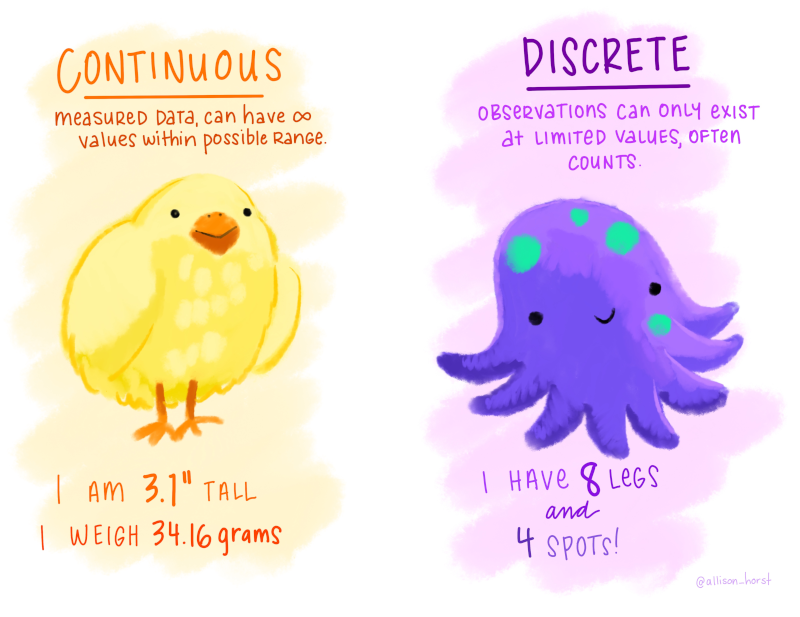
\includegraphics{figures/continuous_discrete.png}\end{minipage}%
%
\begin{minipage}{0.55\linewidth}
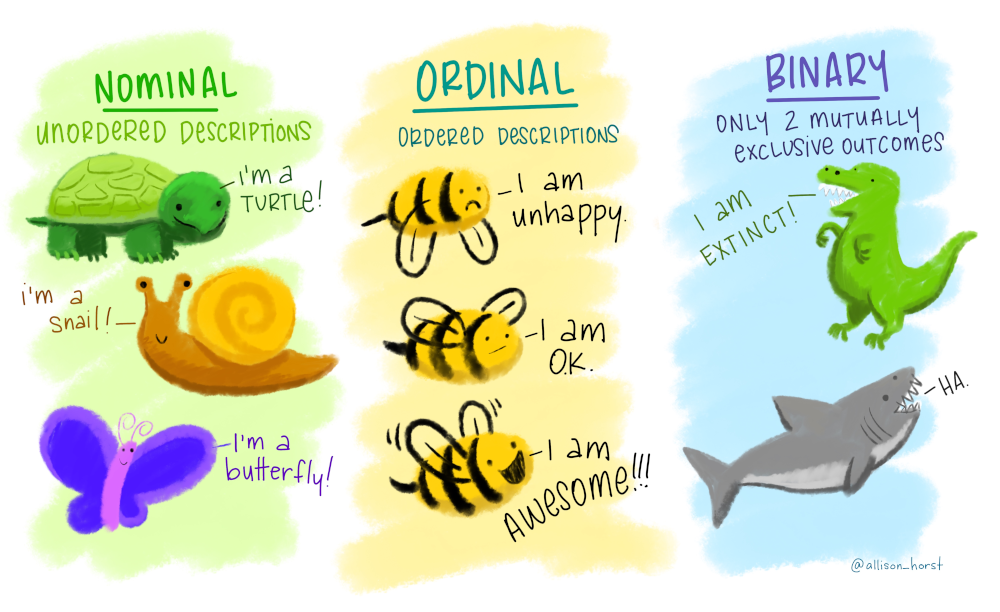
\includegraphics{figures/nominal_ordinal_binary.png}\end{minipage}%

\caption{\label{fig-types-variables}Illustrations par Allison Horst de
variables numériques (gauche) et catégorielles (droite).}

\end{figure}%

On distingue deux types de variables quantitatives:

\begin{itemize}
\tightlist
\item
  une variable discrète prend un nombre dénombrable de valeurs; ce sont
  souvent des variables de dénombrement ou des variables dichotomiques.
\item
  une variable continue peut prendre (en théorie) une infinité de
  valeurs, même si les valeurs mesurées sont arrondies ou mesurées avec
  une précision limitée (temps, taille, masse, vitesse, salaire). Dans
  bien des cas, nous pouvons considérer comme continues des variables
  discrètes si elles prennent un assez grand nombre de valeurs.
\end{itemize}

Les variables catégorielles représentent un ensemble fini de
possibilités. On les regroupe en deux types, pour lesquels on ne fera
pas de distinction:

\begin{itemize}
\tightlist
\item
  nominales s'il n'y a pas d'ordre entre les modalités (sexe, couleur,
  pays d'origine) ou
\item
  ordinale (échelle de Likert, tranche salariale).
\end{itemize}

La codification des modalités des variables catégorielle est arbitraire;
en revanche, on préservera l'ordre lorsqu'on représentera graphiquement
les variables ordinales. Lors de l'estimation, chaque variable
catégorielle doit est transformée en un ensemble d'indicateurs binaires:
il est donc essentiel de déclarer ces dernières dans votre logiciel
statistique, surtout si elles sont encodées dans la base de données à
l'aide de valeurs entières.

\section{Validation des données.}\label{validation-des-donnuxe9es.}

Avant de regarder les données, il est souvent utile de se plonger dans
la description de la base de données. Il n'est pas rare que cette
dernière contienne des informations pertinentes sur la codification des
données, par exemple

\begin{itemize}
\tightlist
\item
  telle variable catégorielle est stockée avec des valeurs entières et
  les étiquettes ne sont disponibles que dans la description.
\item
  des valeurs manquantes sont encodées avec \(-1\) (pour les variables
  positives) ou \(999\).
\item
  une variable est une fonction, transformation ou combinaison d'autres
  variables.
\end{itemize}

\section{Graphiques}\label{graphiques}

Le principal type de graphique pour représenter la distribution d'une
variable catégorielle est le diagramme en bâtons, dans lequel la
fréquence de chaque catégorie est présentée sur l'axe des ordonnées
(\(y\)) en fonction de la modalité, sur l'axe des abscisses (\(x\)), et
ordonnées pour des variables ordinales. Cette représentation est en tout
point supérieur au
\href{http://www.perceptualedge.com/articles/08-21-07.pdf}{diagramme en
camembert}, une engeance répandue qui devrait être honnie (notamment
parce que l'humain juge mal les différences d'aires, qu'une simple
rotation change la perception du graphique et qu'il est difficile de
mesurer les proportions) --- ce n'est pas de la tarte!

\begin{Shaded}
\begin{Highlighting}[]
\FunctionTok{library}\NormalTok{(ggplot2)}
\FunctionTok{library}\NormalTok{(patchwork)}
\FunctionTok{library}\NormalTok{(dplyr)}
\FunctionTok{data}\NormalTok{(renfe, }\AttributeTok{package =} \StringTok{"hecmodstat"}\NormalTok{)}
\NormalTok{g1 }\OtherTok{\textless{}{-}}\NormalTok{ renfe }\SpecialCharTok{|\textgreater{}}
    \FunctionTok{count}\NormalTok{(classe) }\SpecialCharTok{|\textgreater{}}
    \FunctionTok{mutate}\NormalTok{(}\AttributeTok{classe =}\NormalTok{ forcats}\SpecialCharTok{::}\FunctionTok{fct\_reorder}\NormalTok{(classe, n))  }\SpecialCharTok{|\textgreater{}}
\FunctionTok{ggplot}\NormalTok{(}\AttributeTok{mapping =} \FunctionTok{aes}\NormalTok{(}\AttributeTok{y =}\NormalTok{ classe, }\AttributeTok{x =}\NormalTok{ n)) }\SpecialCharTok{+} 
    \FunctionTok{geom\_col}\NormalTok{() }\SpecialCharTok{+} 
    \FunctionTok{labs}\NormalTok{(}\AttributeTok{subtitle =} \StringTok{"classe"}\NormalTok{, }
    \AttributeTok{x =} \StringTok{"dénombrement"}\NormalTok{, }
    \AttributeTok{y =} \StringTok{""}\NormalTok{)}
\NormalTok{g2 }\OtherTok{\textless{}{-}}\NormalTok{ renfe }\SpecialCharTok{|\textgreater{}}
    \FunctionTok{count}\NormalTok{(type) }\SpecialCharTok{|\textgreater{}}
    \FunctionTok{mutate}\NormalTok{(}\AttributeTok{type =}\NormalTok{ forcats}\SpecialCharTok{::}\FunctionTok{fct\_reorder}\NormalTok{(type, n))  }\SpecialCharTok{|\textgreater{}}
\FunctionTok{ggplot}\NormalTok{(}\AttributeTok{mapping =} \FunctionTok{aes}\NormalTok{(}\AttributeTok{y =}\NormalTok{ type, }\AttributeTok{x =}\NormalTok{ n)) }\SpecialCharTok{+} 
    \FunctionTok{geom\_col}\NormalTok{() }\SpecialCharTok{+} 
    \FunctionTok{labs}\NormalTok{(}\AttributeTok{subtitle =} \StringTok{"type de train"}\NormalTok{, }
         \AttributeTok{x =} \StringTok{"dénombrement"}\NormalTok{, }
         \AttributeTok{y =} \StringTok{""}\NormalTok{)}
\NormalTok{g1 }\SpecialCharTok{+}\NormalTok{ g2}
\end{Highlighting}
\end{Shaded}

\begin{figure}[ht!]

\centering{

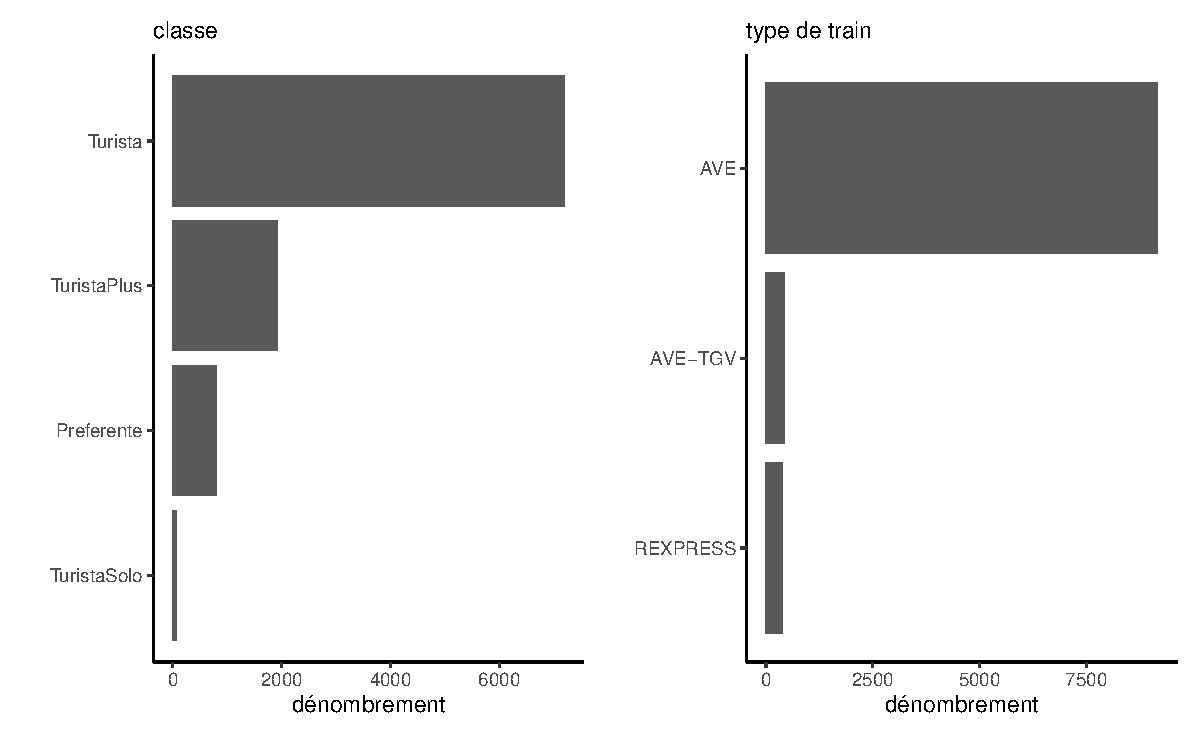
\includegraphics[width=1\textwidth,height=\textheight]{analyseexploratoire_files/figure-pdf/fig-barplotrenfe-1.pdf}

}

\caption{\label{fig-barplotrenfe}Diagramme en bâtons pour la classe des
billets de trains du jeu de données Renfe.}

\end{figure}%

Puisque les variables continues peuvent prendre autant de valeurs
distinctes qu'il y a d'observations, on ne peut simplement compter le
nombre d'occurrence par valeur unique. On regroupera plutôt dans un
certain nombre d'intervalle, en discrétisant l'ensemble des valeurs en
classes pour obtenir un histogramme. Le nombre de classes dépendra du
nombre d'observations si on veut que l'estimation ne soit pas impactée
par le faible nombre d'observations par classe: règle générale, le
nombre de classes ne devrait pas dépasser \(\sqrt{n}\), où \(n\) est le
nombre d'observations de l'échantillon. On obtiendra la fréquence de
chaque classe, mais si on normalise l'histogramme (de façon à ce que
l'aire sous les bandes verticales égale un), on obtient une
approximation discrète de la fonction de densité. Faire varier le nombre
de classes permet parfois de faire apparaître des caractéristiques de la
variable (notamment la multimodalité, l'asymmétrie et les arrondis).

Puisque qu'on groupe les observations en classe pour tracer
l'histogramme, il est difficile de voir l'étendue des valeurs que prenne
la variable: on peut rajouter des traits sous l'histogramme pour
représenter les valeurs uniques prises par la variable, tandis que la
hauteur de l'histogramme nous renseigne sur leur fréquence relative.

\begin{Shaded}
\begin{Highlighting}[]
\NormalTok{renfe }\SpecialCharTok{|\textgreater{}}
  \FunctionTok{subset}\NormalTok{(tarif }\SpecialCharTok{==} \StringTok{"Promo"}\NormalTok{) }\SpecialCharTok{|\textgreater{}}
  \FunctionTok{ggplot}\NormalTok{(}\FunctionTok{aes}\NormalTok{(}\AttributeTok{x =}\NormalTok{ prix)) }\SpecialCharTok{+} 
    \FunctionTok{geom\_histogram}\NormalTok{(}\FunctionTok{aes}\NormalTok{(}\AttributeTok{y =} \FunctionTok{after\_stat}\NormalTok{(density)), }
                   \AttributeTok{bins =} \DecValTok{30}\NormalTok{) }\SpecialCharTok{+}
    \FunctionTok{geom\_rug}\NormalTok{(}\AttributeTok{sides =} \StringTok{"b"}\NormalTok{) }\SpecialCharTok{+} 
    \FunctionTok{labs}\NormalTok{(}\AttributeTok{x =} \StringTok{"prix de billets au tarif Promo (en euros)"}\NormalTok{, }
         \AttributeTok{y =} \StringTok{"densité"}\NormalTok{) }
\end{Highlighting}
\end{Shaded}

\begin{figure}[ht!]

\centering{

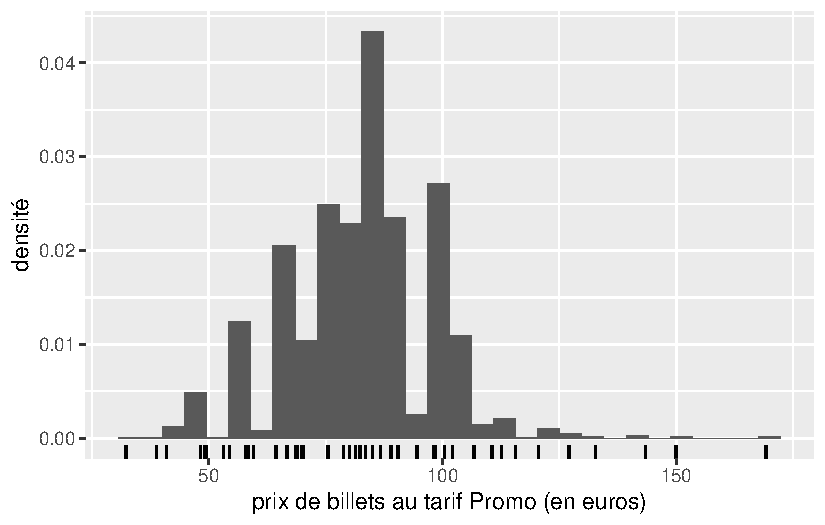
\includegraphics[width=1\textwidth,height=\textheight]{analyseexploratoire_files/figure-pdf/fig-histrenfe-1.pdf}

}

\caption{\label{fig-histrenfe}Histogramme du prix des billets au tarif
Promo de trains du jeu de données Renfe}

\end{figure}%

Une boîte à moustaches représente graphiquement cinq statistiques
descriptives.

\begin{itemize}
\tightlist
\item
  La boîte donne les 1e, 2e et 3e quartiles \(q_1, q_2, q_3\). Il y a
  donc 50\% des observations sont au-dessus/en-dessous de la médiane
  \(q_2\) qui sépare en deux la boîte.
\item
  La longueur des moustaches est moins de \(1.5\) fois l'écart
  interquartile \(q_3-q_1\) (tracée entre 3e quartile et le dernier
  point plus petit que \(q_3+1.5(q_3-q_1)\), etc.)
\item
  Les observations au-delà des moustaches sont encerclées. Notez que
  plus le nombre d'observations est élevé, plus le nombres de valeurs
  extrême augmente. C'est un défaut de la boîte à moustache, qui a été
  conçue pour des jeux de données qui passeraient pour petits selon les
  standards actuels.
\end{itemize}

\begin{figure}[ht!]

\centering{

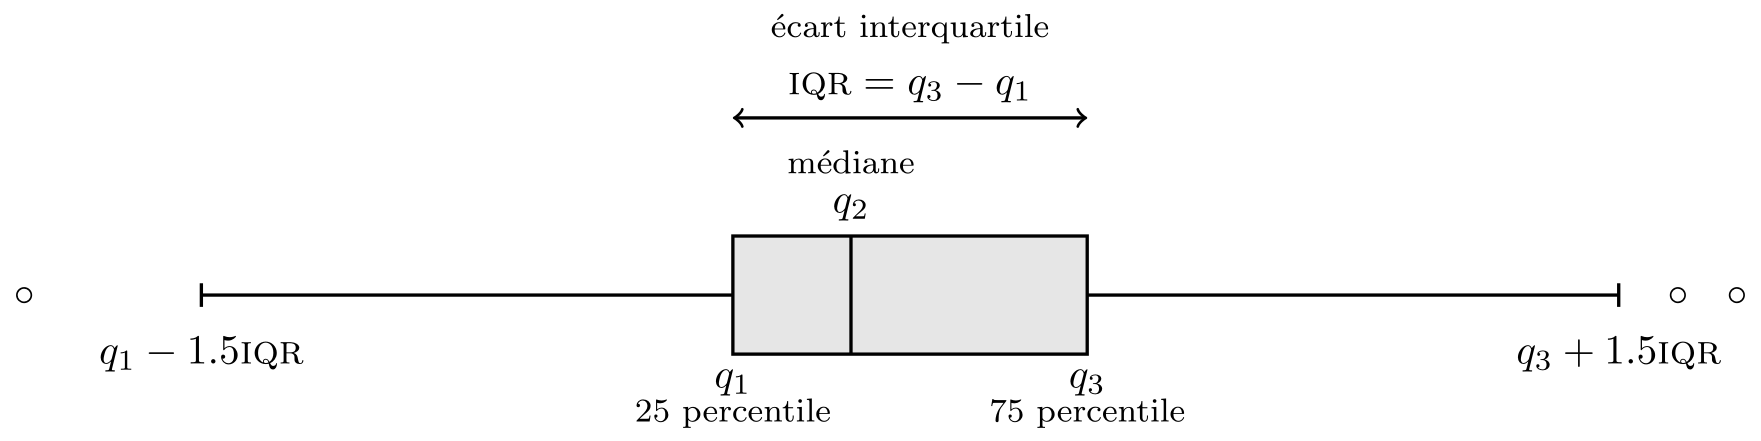
\includegraphics[width=1\textwidth,height=\textheight]{figures/01-intro-boiteamoustache.png}

}

\caption{\label{fig-boiteamoustache}Boîte à moustache.}

\end{figure}%

On peut représenter la distribution d'une variable réponse continue en
fonction d'une variable catégorielle en traçant une boîte à moustaches
pour chaque catégorie et en les disposant côte-à-côte. Une troisième
variable catégorielle peut être ajoutée par le biais de couleurs, comme
dans la Figure~\ref{fig-histboxplot}.

\begin{Shaded}
\begin{Highlighting}[]
\NormalTok{renfe }\SpecialCharTok{|\textgreater{}} 
   \FunctionTok{subset}\NormalTok{(tarif }\SpecialCharTok{==} \StringTok{"Promo"}\NormalTok{) }\SpecialCharTok{|\textgreater{}}
   \FunctionTok{ggplot}\NormalTok{(}\FunctionTok{aes}\NormalTok{(}\AttributeTok{y =}\NormalTok{ prix, }\AttributeTok{x =}\NormalTok{ classe, }\AttributeTok{col =}\NormalTok{ type)) }\SpecialCharTok{+} 
    \FunctionTok{geom\_boxplot}\NormalTok{() }\SpecialCharTok{+} 
    \FunctionTok{labs}\NormalTok{(}\AttributeTok{y =} \StringTok{"prix (en euros)"}\NormalTok{, }
         \AttributeTok{col =} \StringTok{"type de train"}\NormalTok{) }\SpecialCharTok{+} 
    \FunctionTok{theme}\NormalTok{(}\AttributeTok{legend.position =} \StringTok{"bottom"}\NormalTok{)}
\end{Highlighting}
\end{Shaded}

\begin{figure}[ht!]

\centering{

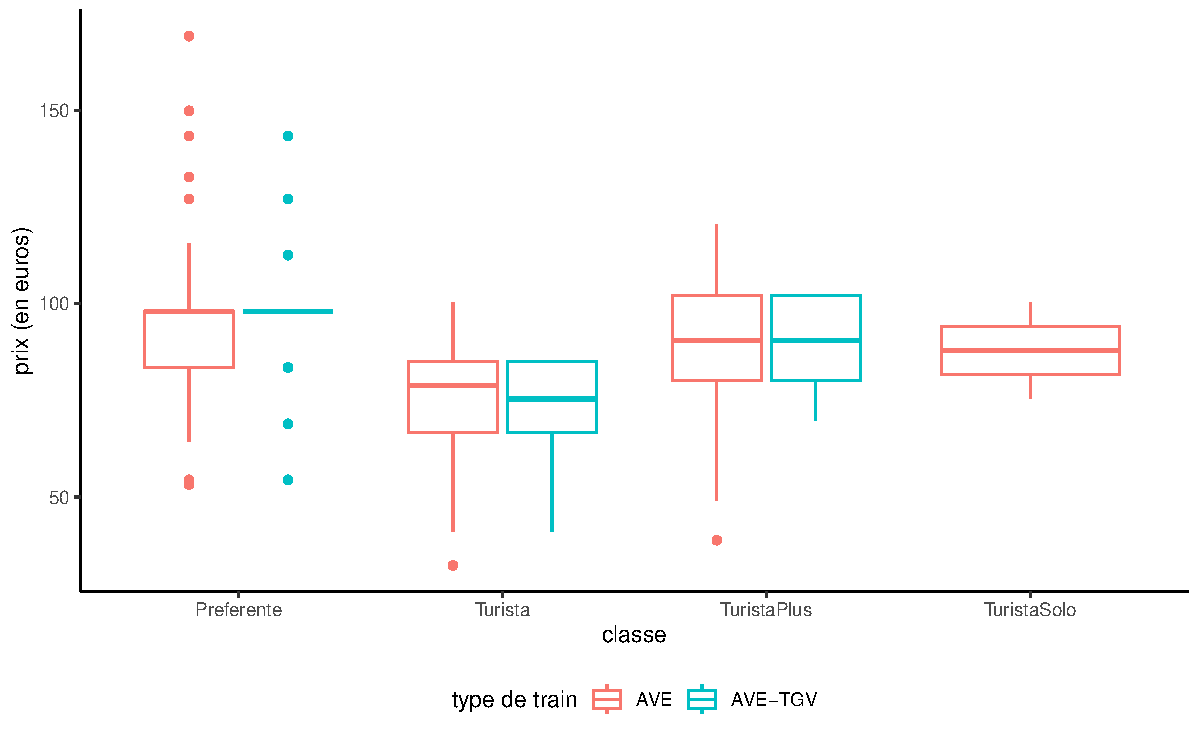
\includegraphics[width=1\textwidth,height=\textheight]{analyseexploratoire_files/figure-pdf/fig-histboxplot-1.pdf}

}

\caption{\label{fig-histboxplot}Boîte à moustaches du prix des billets
au tarif Promo en fonction de la classe pour le jeu de données Renfe.}

\end{figure}%

Si on veut représenter la covariabilité de deux variables continues, on
utilise un nuage de points où chaque variable est représentée sur un axe
et chaque observation donne la coordonnée des points. Si la
représentation graphique est dominée par quelques valeurs très grandes,
une transformation des données peut être utile: vous verrez souvent des
données positives à l'échelle logarithmique.

Plutôt que de décrire plus en détail le processus de l'analyse
exploratoire, on présente un exemple qui illustre le cheminement habitue
sur les données de trains de la Renfe introduites précédemment.

\section{Exemple}\label{exemple}

La première étape consisterait à lire la description de la base de
données. Le jeu de données \texttt{renfe} contient les variables
suivantes:

\begin{itemize}
\tightlist
\item
  \texttt{prix}: prix du billet (en euros);
\item
  \texttt{dest}: indicateur binaire du trajet, soit de Barcelone vers
  Madrid (\texttt{0}) ou de Madrid vers Barcelone (\texttt{1});
\item
  \texttt{tarif}: variable catégorielle indiquant le tarif du billet, un
  parmi \texttt{AdultoIda}, \texttt{Promo} et \texttt{Flexible};
\item
  \texttt{classe}: classe du billet, soit \texttt{Preferente},
  \texttt{Turista}, \texttt{TuristaPlus} ou \texttt{TuristaSolo};
\item
  \texttt{type}: variable catégorielle indiquant le type de train, soit
  Alta Velocidad Española (\texttt{AVE}), soit Alta Velocidad Española
  conjointement avec TGV (un partenariat entre la SNCF et Renfe pour les
  trains à destination ou en provenance de Toulouse) \texttt{AVE-TGV},
  soit les trains régionaux \texttt{REXPRESS}; seuls les trains
  étiquetés \texttt{AVE} ou \texttt{AVE-TGV} sont des trains à grande
  vitesse.
\item
  \texttt{duree}: longueur annoncée du trajet (en minutes);
\item
  \texttt{jour} entier indiquant le jour de la semaine du départ allant
  de dimanche (\texttt{1}) à samedi (\texttt{7}).
\end{itemize}

Il n'y a pas de valeurs manquantes et un aperçu des données
(\texttt{head(renfe)}) montre qu'elles sont en format long, ce qui veut
dire que chaque ligne contient une seule valeur pour la variable
réponse, ici le prix d'un billet de train. On entame l'analyse
exploratoire avec des questions plutôt vagues, par exemple

\begin{enumerate}
\def\labelenumi{\arabic{enumi}.}
\tightlist
\item
  Quels sont les facteurs déterminant le prix et le temps de parcours?
\item
  Est-ce que le temps de parcours est le même peut importe le type de
  train?
\item
  Quelles sont les caractéristiques distinctives des types de train?
\item
  Quelles sont les principales différences entre les tarifs?
\end{enumerate}

À l'exception de \texttt{prix} et de \texttt{duree}, toutes les
variables explicatives sont catégorielles. La variable \texttt{jour}
prends des valeurs entre 1 et 7; s'en souvenir pour éviter les mauvaises
surprises ultérieures. En analysant le nombre de trains dans les
catégories, on remarque qu'il y a autant de billets de type
\texttt{REXPRESS} que le nombre de billets au tarif \texttt{AdultoIda}.
On peut faire le décompte par catégorie avec un tableau de contingence,
qui compte le nombre respectif dans chaque sous-catégorie. Dans la base
de données Renfe, tous les billets pour les RegioExpress sont vendus au
tarif \texttt{AdultoIda} en classe \texttt{Turista}. Le nombre de
billets est minime, à peine 397 sur 10000. Cela suggère une nouvelle
question: pourquoi ces trains sont-ils si peu populaires?

On remarque également que seulement 17 temps de parcours sont affichés
sur les billets. On peut donc penser que la durée affichée sur le billet
(en minutes) est le temps de trajet annoncé. La majeure partie (15 sur
17) des temps de parcours sont sous la barre des 3h15, hormis deux qui
dépassent les 9h! Selon Google Maps, les deux villes sont distantes de
615km par la route, 500km à vol d'oiseau. Cela implique que,
vraisemblablement, certains trains dépassent les 200km/h, tandis que
d'autres vont plutôt à 70km/h. Quels sont ces trains plus lent? La
variable \texttt{type} codifie probablement ce fait, et permet de voir
que ce sont les trains RegioExpress qui sont dans cette catégorie.

Aller de Madrid à Barcelone à l'aide d'un train régulier prend 18
minutes de plus. Avec plus de 9h de trajet, pas étonnant donc que ces
billets soient peu courus. Encore plus frappant, on note que le prix des
billets est fixe: 43.25 euros peu importe que le trajet soit aller ou
retour. C'est probablement la trouvaille la plus importante jusqu'à
maintenant, car les billets de train de type RegioExpress ne forment pas
un échantillon: il n'y a aucune variabilité! On aurait également pu
découvrir cette anomalie en traçant une boîte à moustaches du prix en
fonction du type de train.

\begin{Shaded}
\begin{Highlighting}[]
\FunctionTok{ggplot}\NormalTok{(}\AttributeTok{data =}\NormalTok{ renfe, }
       \AttributeTok{mapping =} \FunctionTok{aes}\NormalTok{(}\AttributeTok{x =}\NormalTok{ type, }\AttributeTok{y =}\NormalTok{ prix, }\AttributeTok{col =}\NormalTok{ dest)) }\SpecialCharTok{+} 
  \FunctionTok{geom\_boxplot}\NormalTok{() }\SpecialCharTok{+} 
  \FunctionTok{labs}\NormalTok{(}\AttributeTok{y =} \StringTok{"prix (en euros)"}\NormalTok{,}
       \AttributeTok{x =} \StringTok{"type de train"}\NormalTok{,}
       \AttributeTok{color =} \StringTok{"destination"}\NormalTok{) }\SpecialCharTok{+}
  \FunctionTok{theme}\NormalTok{(}\AttributeTok{legend.position =} \StringTok{"bottom"}\NormalTok{)}
\end{Highlighting}
\end{Shaded}

\begin{figure}[ht!]

\centering{

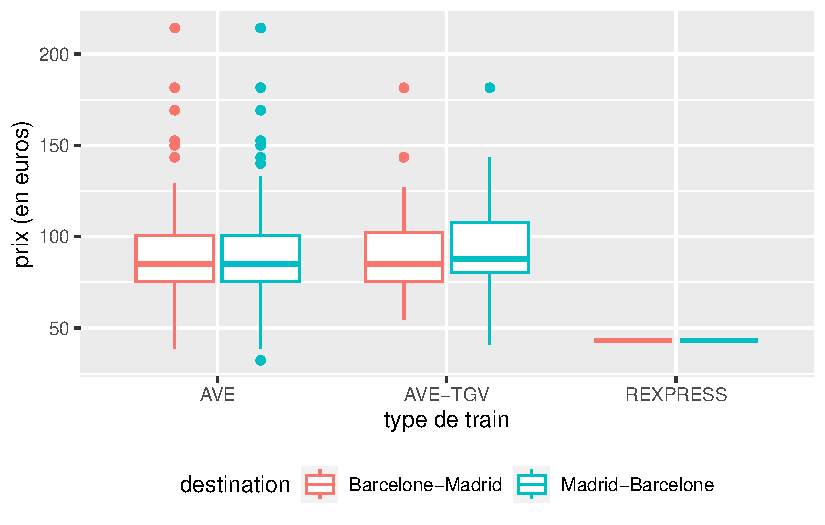
\includegraphics[width=1\textwidth,height=\textheight]{analyseexploratoire_files/figure-pdf/fig-renfe-aed4-1.pdf}

}

\caption{\label{fig-renfe-aed4}Boîte à moustaches du prix de billets de
train de Renfe en fonction de la destination et du type de train.}

\end{figure}%

On pourrait soupçonner que les trains étiquetés \texttt{AVE} sont plus
rapides, sachant que c'est l'acronyme de \emph{Alta Velocidad Española},
littéralement haute vitesse espagnole. Qu'en est-il des distinctions
entre les deux types de trains étiquetés AVE? Selon
\href{https://www.renfe-sncf.com/rw-en/services/a-unique-experience/Pages/services.aspx}{le
site de la SNCF}, les trains AVE-TGV sont des partenariats entre la
Renfe et la SNCF et effectuent des liaisons entre la France et
l'Espagne.

Les prix sont beaucoup plus élevés, en moyenne plus de deux fois plus
que les trains régionaux. Les écarts de prix importants (l'écart type
est de 20 euros) indique qu'il y a peut-être d'autres sources
d'hétérogénéité, mais on pourrait soupçonner que la Renfe pratique la
tarification dynamique. Il y un seul temps de parcours prévu pour les
trains AVE-TGV. On ne note pas de différence de prix notable selon la
direction ou le type de train grande vitesse, mais peut-être que les
tarifs ou la classe disponibles diffèrent selon que le train ou non est
en partenariat avec la compagnie française.

On n'a pas encore considéré le tarif et la classe des billets, hormis
pour les trains RegioExpress. On voit dans la
Figure~\ref{fig-renfe-aed7} une forte différente dans l'hétérogénéité
des prix selon le tarif; le tarif Promo prend plusieurs valeurs
distinctes, tandis que les tarifs AdultoIda et Flexible semblent ne
prendre que quelques valeurs. La première classe (\texttt{Preferente})
est plus chère et il y a moins d'observations dans ce groupe. La classe
Turista est la classe la moins dispendieuse et la plus populaire.
\href{http://web.archive.org/web/20161111134241/http://www.renfe.com/viajeros/tarifas/billete_promo.html}{\texttt{TuristaPlus}}
offre plus de confort, tandis que \texttt{TuristaSolo} permet d'obtenir
un siège individuel.

Côté tarif,
\href{http://web.archive.org/web/20161111134241/http://www.renfe.com/viajeros/tarifas/billete_promo.html}{Promo}
et
\href{http://web.archive.org/web/20161110220249/http://www.renfe.com/viajeros/tarifas/billete_promoplus.html}{PromoPlus}
permette d'obtenir des rabais pouvant aller jusqu'à respectivement 70\%
et 65\%. Les annulations et changements ne sont pas possibles avec
Promo, mais disponibles avec PromoPlus moyennant une pénalité équivalent
à 30-20\% du prix du billet. Le tarif
\href{http://web.archive.org/web/20161108192609/http://www.renfe.com/viajeros/tarifas/billete_flexible.html}{Flexible}
est disponible au même prix que les billets réguliers, avec des
bénéfices additionnels.

\begin{figure}[ht!]

\centering{

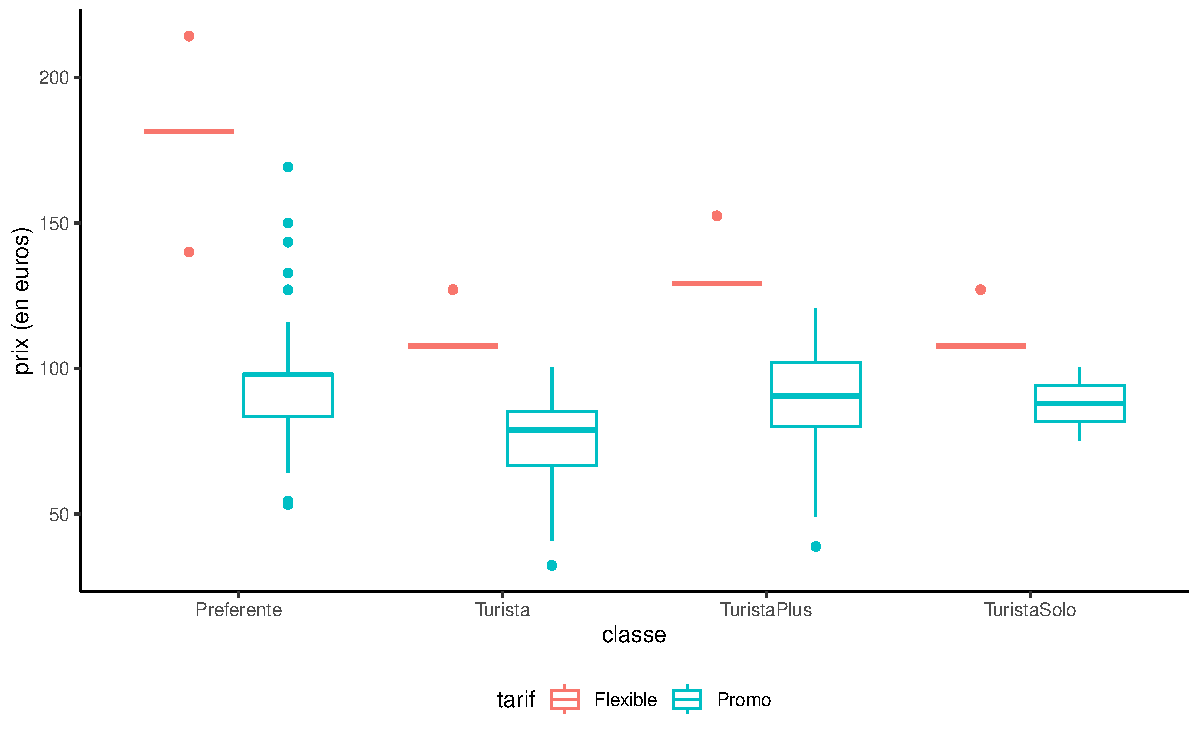
\includegraphics[width=1\textwidth,height=\textheight]{analyseexploratoire_files/figure-pdf/fig-renfe-aed6-1.pdf}

}

\caption{\label{fig-renfe-aed6}Boîte à moustaches du prix en fonction du
tarif et de la classe de billets de trains à haute vitesse de la Renfe.}

\end{figure}%

\begin{figure}[ht!]

\centering{

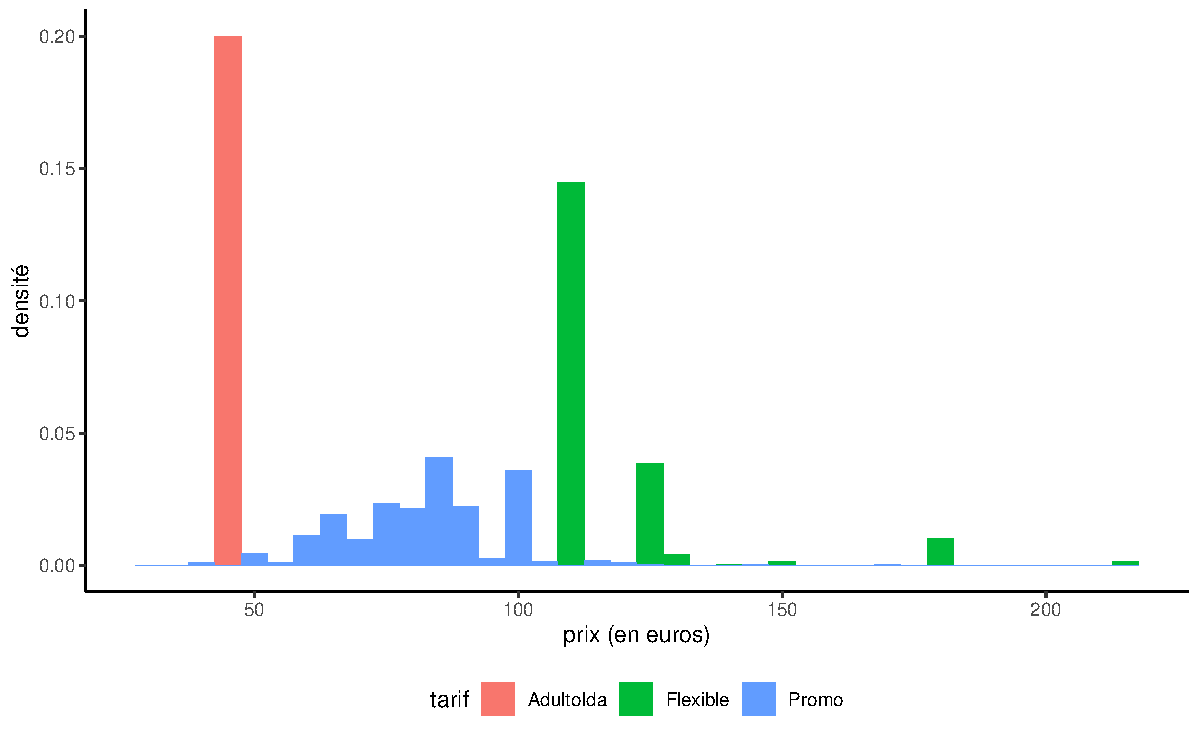
\includegraphics[width=1\textwidth,height=\textheight]{analyseexploratoire_files/figure-pdf/fig-renfe-aed7-1.pdf}

}

\caption{\label{fig-renfe-aed7}Histogrammes du prix en fonction du tarif
de billets de trains de la Renfe.}

\end{figure}%

\begin{Shaded}
\begin{Highlighting}[]
\NormalTok{renfe }\SpecialCharTok{|\textgreater{}}
\NormalTok{  dplyr}\SpecialCharTok{::}\FunctionTok{subset}\NormalTok{(tarif  }\SpecialCharTok{==} \StringTok{"Flexible"}\NormalTok{) }\SpecialCharTok{|\textgreater{}}
\NormalTok{  dplyr}\SpecialCharTok{::}\FunctionTok{count}\NormalTok{(prix, classe)}
\end{Highlighting}
\end{Shaded}

\begin{table}

\caption{\label{tbl-renfeaedrep}Nombre de billets au tarif Flexible
selon le prix de vente.}

\centering{

\begin{tabular}[t]{rlr}
\toprule
prix & classe & n\\
\midrule
108 & Turista & 1050\\
108 & TuristaSolo & 67\\
127 & Turista & 285\\
127 & TuristaSolo & 9\\
129 & TuristaPlus & 31\\
\addlinespace
140 & Preferente & 2\\
152 & TuristaPlus & 10\\
182 & Preferente & 78\\
214 & Preferente & 12\\
\bottomrule
\end{tabular}

}

\end{table}%

On note que la répartition des prix pour les billets de classe Flexible
est inhabituelle. Notre boîte à moustaches est écrasée et l'écart
interquartile semble nul, même si quelques valeurs inexpliquées sont
aussi présentes. L'écrasante majorité des billets Flexibles sont en
classe Turista, donc ça pourrait être dû à un (trop) faible nombre de
billets dans chaque catégorie. On peut rejeter cette hypothèse en
calculant le nombre de trains au tarif Flexible pour les différents
types de billets, comme dans le Tableau~\ref{tbl-renfeaedrep}. Ni la
durée, ni le type de train, ni la destination n'expliquent pas pourquoi
le prix de certains billets Flexibles est plus faible ou élevés. Le prix
des billets Promo est plus faible, et les billets au tarif Preferente
(la première classe) sont plus élevés.

On peut résumer notre brève analyse exploratoire:

\begin{itemize}
\tightlist
\item
  plus de 91\% des trains sont des trains à grande vitesse AVE.
\item
  le temps de trajet dépend du type de train: les trains à grande
  vitesse mettent 3h20 au maximum pour relier Madrid et Barcelone.
\item
  les temps de trajets sont ceux annoncés (variable discrète avec 17
  valeurs uniques, dont 13 pour les trains AVE)
\item
  le prix de trains RegioExpress est fixe (43.25€); tous ces billets
  sont dans la classe Turista et au tarif Adulto Ida. 57\% de ces trains
  vont de Barcelone à Madrid. La durée du trajet pour les RegioExpress
  est de 9h22 de Barcelona à Madrid, 18 minutes de plus que dans l'autre
  direction.
\item
  les billets en classe \texttt{Preferente} sont plus chers et moins
  fréquents. La classe \texttt{Turista} est la classe la moins
  dispendieuse et la plus populaire. \texttt{TuristaPlus} offre plus de
  confort, tandis que \texttt{TuristaSolo} permet d'obtenir un siège
  individuel.
\item
  selon le site web de la Renfe, les billets au tarif \texttt{Flexible}
  « viennent avec des offres additionnelles qui permettent au passagers
  d'échanger leurs billets ou annuler s'ils manquent leurs trains. »; en
  contrepartie, ces billets sont plus chers et leur tarif est fixe sauf
  une poignée de billets dont le prix reste inexpliqué.
\item
  la distribution des prix des billets de TGV au tarif \texttt{Promo}
  est plus ou moins symmétrique, tandis que les billets au tarif
  \texttt{Flexible} apparaissent tronqués à gauche (le prix minimum pour
  ces billets est 107.7€ dans l'échantillon).
\item
  la Renfe pratique la tarification dynamique pour les billets au tarif
  promotionnel \texttt{Promo}: ces derniers peuvent être jusqu'à 70\%
  moins chers que les billets à prix régulier lorsqu'achetés via
  l'agence officielle ou le site de Renfe. Ces billets ne peuvent être
  ni remboursés, ni échangés.
\item
  il n'y a pas d'indication à effet de quoi les prix varient selon la
  direction du trajet.
\end{itemize}

\subsection{Commentaire sur les
graphiques}\label{commentaire-sur-les-graphiques}

Si vous incluez un graphique (ou un tableau), il est important d'ajouter
une légende qui décrit le graphique et le résume, les noms de variables
(avec les unités) sur les axes, mais aussi de soigner le rendu et le
formatage pour obtenir un produit fini propre, lisible et cohérent: en
particulier, votre description devrait coïncider avec le rendu. Votre
graphique raconte une histoire, aussi prenez-soin que cette dernière
soit nécessaire et attrayante.

\begin{tcolorbox}[enhanced jigsaw, bottomrule=.15mm, toptitle=1mm, opacityback=0, title=\textcolor{quarto-callout-note-color}{\faInfo}\hspace{0.5em}{En résumé}, left=2mm, bottomtitle=1mm, colbacktitle=quarto-callout-note-color!10!white, colback=white, breakable, toprule=.15mm, coltitle=black, arc=.35mm, opacitybacktitle=0.6, colframe=quarto-callout-note-color-frame, titlerule=0mm, leftrule=.75mm, rightrule=.15mm]

\begin{itemize}
\tightlist
\item
  Une base de données est normalement constituée de plusieurs variables
  (colonnes); les lignes représentent les différentes observations.
\item
  On classifie grossièrement les variables en variables catégorielles
  (nominales, ordinales ou binaires) et numériques (continues,
  entières).
\item
  L'analyse exploratoire est une procédure dynamique qui sert à mieux
  comprendre les données pour proposer des modèles adéquats. Elle
  consiste à poser des questions et à raffiner les conclusions à l'aide
  de tableaux résumés et de graphique.
\item
  Le nettoyage et la validation des données est la première étape de
  toute analyse. On peut formuler nos attentes et l'utiliser pour
  vérifier de la conformité de notre base de données (en utilisant des
  outils comme le
  \href{https://github.com/rich-iannone/pointblank}{paquet
  \texttt{pointblank}}).
\item
  Une bonne compréhension des données est nécessaire avant d'envisager
  la modélisation.
\item
  Il faut déclarer correctement les variables explicatives catégorielles
  (souvent encodées avec des entiers).
\item
  L'utilisation de graphiques est privilégiée par rapport aux tableaux:
  une image vaut mille mots.
\item
  Les graphiques usuels employés sont l'histogramme et la boîte à
  moustaches (données numériques) et le diagramme à bande (données
  catégorielles). L'utilisation de diagramme circulaires est à
  proscrire.
\item
  On peut utiliser la couleur, la forme ou la taille comme dimensions
  additionnelles.
\item
  Toujours utiliser une palette de couleurs pour daltoniens.
\item
  Un graphique devrait toujours inclure une légende globale décrivant la
  représentation (en plus d'être discuté dans le texte), une légende
  pour les axes et des unités. Les caractères doivent être lisibles
  (suffisamment grands).
\item
  Une analyse exploratoire inclut un résumé des principales trouvailles.
\end{itemize}

\end{tcolorbox}

\bookmarksetup{startatroot}

\chapter{Sélection de variables et de modèles}\label{selection-modele}

Ce chapitre présente des principes, outils et méthodes très généraux
pour choisir un « bon » modèle. Nous allons principalement utiliser la
régression linéaire pour illustrer les méthodes en supposant que tout le
monde connaît ce modèle de base. Les méthodes présentées sont en
revanche très générales et peuvent être appliquées avec n'importe quel
autre modèle (régression logistique, arbres de classification et
régression, réseaux de neurones, analyse de survie, etc.)

L'expression « sélection de variables » fait référence à la situation où
l'on cherche à sélectionner un sous-ensemble de variables à inclure dans
notre modèle à partir d'un ensemble de variables \(X_1, \ldots, X_p\).
Le terme variable ici inclut autant des variables distinctes que des
transformations d'une ou plusieurs variables.

Par exemple, supposons que les variables \(\texttt{age}\),
\(\texttt{sexe}\) et \(\texttt{revenu}\) soient trois variables
explicatives disponibles. Nous pourrions alors considérer choisir entre
ces trois variables. Mais aussi, nous pourrions considérer inclure
\(\texttt{age}^2\), \(\texttt{age}^3\), \(\log(\texttt{age})\), etc.
Nous pourrions aussi considérer des termes d'interactions entre les
variables, comme \(\texttt{age} \cdot \texttt{revenu}\) ou
\(\texttt{age}\cdot\texttt{revenu}\cdot\texttt{sexe}\). Le problème est
alors de trouver un bon sous-ensemble de variables parmi toutes celles
considérées.

L'expression « sélection de modèle » est un peu plus générale. D'une
part, elle inclut la sélection de variables car, pour une famille de
modèles spécifiques (régression linéaire par exemple), choisir un
sous-ensemble de variables revient à choisir un modèle. D'autre part,
elle fait référence à la situation où l'on cherche à trouver le meilleur
modèle parmi des modèles de natures différentes. Par exemple, on
pourrait choisir entre une régression linéaire, un arbre de régression,
une forêt aléatoire, un réseau de neurones, etc.

\section{Sélection de variables et de modèles selon les buts de
l'étude}\label{suxe9lection-de-variables-et-de-moduxe8les-selon-les-buts-de-luxe9tude}

Nous disposons d'une variable réponse \(Y\) et d'un ensemble de
variables explicatives \(X_1, \ldots, X_p\). L'attitude à adopter dépend
des buts de l'étude.

\begin{itemize}
\tightlist
\item
  \textbf{1e situation}: On veut développer un modèle pour faire des
  prédictions sans qu'il soit important de tester formellement les
  effets des paramètres individuels.
\end{itemize}

Dans ce cas, on désire seulement que notre modèle soit performant pour
prédire des valeurs futures de \(Y\). On peut alors baser notre choix de
variable (et de modèle) en utilisant des outils qui nous guiderons quant
aux performances prédictives futures du modèle (voir \(\mathsf{AIC}\),
\(\mathsf{BIC}\) et validation croisée plus loin). On pourra enlever ou
rajouter des variables et des transformations de variables au besoin
afin d'améliorer les performances prédictives. Les méthodes que nous
allons voir concernent essentiellement ce contexte.

\begin{itemize}
\tightlist
\item
  \textbf{2e situation}: On veut développer un modèle pour estimer les
  effets de certaines variables sur notre \(Y\) et tester des hypothèses
  de recherche spécifiques concernant certaines variables.
\end{itemize}

Dans ce cas, il est préférable de spécifier le modèle dès le départ
selon des considérations scientifiques et de s'en tenir à lui. Faire une
sélection de variables dans ce cas est dangereux car on ne peut pas
utiliser directement les valeurs-\emph{p} des tests d'hypothèses (ou les
intervalles de confiance sur les paramètres) concernant les paramètres
du modèle final car elles ne tiennent pas compte de la variabilité due
au processus de sélection de variables.

Une bonne planification de l'étude est alors cruciale afin de collecter
les bonnes variables, de spécifier le ou les bons modèles, et de
s'assurer d'avoir suffisamment d'observations pour ajuster le ou les
modèles désirés.

Si procéder à une sélection de variables est quand même nécessaire dans
ce contexte, il est quand même possible de le faire en divisant
l'échantillon en deux. La sélection de variables pourrait être alors
effectuée avec le premier échantillon. Une fois qu'un modèle est retenu,
on pourrait alors réajuster ce modèle avec le deuxième échantillon (sans
faire de sélection de variables cette fois-ci). L'inférence sur les
paramètres (valeurs-\emph{p}, etc.) sera alors valide. Le désavantage
ici qu'il faut avoir une très grande taille d'échantillon au départ afin
d'être en mesure de le diviser en deux.

\section{Estimation de la
performance}\label{estimation-de-la-performance}

Il est préférable d'avoir un modèle un peu trop complexe qu'un modèle
trop simple. Plaçons-nous dans le contexte de la régression linéaire et
supposons que le vrai modèle est inclus dans le modèle qui a été ajusté.
Il y a donc des variables en trop dans le modèle qui a été ajusté: ce
dernier est dit surspécifié.

Par exemple, supposons que le vrai modèle est
\(Y=\beta_0+\beta_1X_1+\varepsilon\) mais que c'est le modèle
\(Y=\beta_0+\beta_1X_1+\beta_2X_2+\varepsilon\) qui a été ajusté. Dans
ce cas, règle générale, les estimateurs des paramètres et les
prédictions provenant du modèle sont sans biais. Mais leurs variances
estimées seront un peu plus élevées car on estime des paramètres pour
des variables superflues.

Pour illustrer ce point, j'ai simulé des données avec deux variables
explicatives corrélées. Les vrais coefficients du modèle linéaire sont
\(\beta_0 = 20\), \(\beta_1=2\) et \(\beta_2 = 0\).

\begin{table}

\caption{\label{tbl-specification}Surspécification de modèle de
régression linéaire pour des données simulées.}

\begin{minipage}{0.50\linewidth}

\begin{longtable}[]{@{}lrrr@{}}
\caption{modèle correct}\tabularnewline
\toprule\noalign{}
& coef. & borne inf. & borne sup. \\
\midrule\noalign{}
\endfirsthead
\toprule\noalign{}
& coef. & borne inf. & borne sup. \\
\midrule\noalign{}
\endhead
\bottomrule\noalign{}
\endlastfoot
(cst) & 19.95 & 19.28 & 20.62 \\
X1 & 2.74 & 2.55 & 2.94 \\
\end{longtable}

\end{minipage}%
%
\begin{minipage}{0.50\linewidth}

\begin{longtable}[]{@{}lrrr@{}}
\caption{modèle surspécifié}\tabularnewline
\toprule\noalign{}
& coef. & borne inf. & borne sup. \\
\midrule\noalign{}
\endfirsthead
\toprule\noalign{}
& coef. & borne inf. & borne sup. \\
\midrule\noalign{}
\endhead
\bottomrule\noalign{}
\endlastfoot
(cst) & 20.16 & 19.88 & 20.44 \\
X1 & 1.93 & 1.84 & 2.03 \\
X2 & 5.06 & 4.74 & 5.38 \\
\end{longtable}

\end{minipage}%

\end{table}%

Une fois qu'on a obtenu l'estimation des coefficients et les intervalles
de confiance, on peut les comparer aux vraies valeurs (soit
\(\beta_0 = 20\), \(\beta_1=2\) et \(\beta_2 = 0\)) et vérifier si ces
dernières se trouvent dans l'intervalle de confiance. Cela risque en
général de ne pas être le cas si les variables explicatives sont
corrélées, puisqu'elles partagent alors le pouvoir explicatif. Cela,
heureusement, n'a que peu d'incidence sur les prédictions. Le
Tableau~\ref{tbl-specification} indique l'effet pour l'inférence de ces
spécifications (avec des différences d'estimation, mais non de
prédictions, qui sont dues à la colinéarité entre variables).

Supposons à l'inverse qu'il manque des variables dans le modèle ajusté
et que le modèle ajusté est sous-spécifié. Par exemple, supposons que le
vrai modèle est \(Y=\beta_0+\beta_1X_1+\beta_2X_2+\varepsilon\), mais
que c'est le modèle \(Y=\beta_0+\beta_1X_1+\varepsilon\) qui est ajusté.
Dans ce cas, généralement, les estimateurs des paramètres et les
prédictions sont biaisés. Le Tableau~\ref{tbl-specification} montre les
estimations du modèle: les vraies valeurs sont cette fois
\(\beta_0=20\), \(\beta_1 = 2\) et \(\beta_2 = 5\).

\begin{table}

\caption{\label{tbl-specification2}Sous-spécification de modèle de
régression linéaire pour des données simulées.}

\begin{minipage}{0.50\linewidth}

\begin{longtable}[]{@{}lrrr@{}}
\caption{modèle sous-spécifié}\tabularnewline
\toprule\noalign{}
& coefficient & borne inf. & borne sup. \\
\midrule\noalign{}
\endfirsthead
\toprule\noalign{}
& coefficient & borne inf. & borne sup. \\
\midrule\noalign{}
\endhead
\bottomrule\noalign{}
\endlastfoot
(cst) & 20 & 19.74 & 20.31 \\
X1 & 2 & 1.91 & 2.08 \\
\end{longtable}

\end{minipage}%
%
\begin{minipage}{0.50\linewidth}

\begin{longtable}[]{@{}lrrr@{}}
\caption{modèle correct}\tabularnewline
\toprule\noalign{}
& coefficient & borne inf. & borne sup. \\
\midrule\noalign{}
\endfirsthead
\toprule\noalign{}
& coefficient & borne inf. & borne sup. \\
\midrule\noalign{}
\endhead
\bottomrule\noalign{}
\endlastfoot
(cst) & 20.05 & 19.77 & 20.33 \\
X1 & 1.92 & 1.83 & 2.02 \\
X2 & 0.47 & 0.14 & 0.79 \\
\end{longtable}

\end{minipage}%

\end{table}%

Ainsi, il est généralement préférable d'avoir un modèle légèrement
surspécifié qu'un modèle sous-spécifié. Plus généralement, il est
préférable d'avoir un peu trop de variables dans le modèle que de
prendre le risque d'omettre une ou plusieurs variables importantes. Il
faut faire attention et ne pas tomber dans l'excès et avoir un modèle
trop complexe (avec trop de variables inutiles) car il pourrait souffrir
de surajustement (\emph{over-fitting}). Les exemples qui suivent
illustreront ce fait.

\subsection{Surajustement}\label{surajustement}

Cette section traite de l'optimisme de l'évaluation d'un modèle
(\emph{trop beau pour être vrai}) lorsqu'on utilise les mêmes données
qui ont servies à l'ajuster pour évaluer sa performance. Un principe
fondamental lorsque vient le temps d'évaluer la performance prédictive
d'un modèle est le suivant : si on utilise les mêmes observations pour
évaluer la performance d'un modèle que celles qui ont servi à l'ajuster
(à estimer le modèle et ses paramètres), on va surestimer sa
performance. Autrement dit, notre estimation de l'erreur que fera le
modèle pour prédire des observations futures sera biaisée à la baisse.
Ainsi, il aura l'air meilleur que ce qu'il est en réalité. C'est comme
si on demandait à un cinéaste d'évaluer son dernier film. Comme c'est
son film, il n'aura généralement pas un regard objectif. C'est pourquoi
on aura tendance à se fier à l'opinion d'un critique.

On cherchera donc à utiliser des outils et méthodes qui nous donneront
l'heure juste (une évaluation objective) quant à la performance
prédictive d'un modèle.

\subsection{Principes généraux}\label{principes-guxe9nuxe9raux}

Les idées présentées ici seront illustrées à l'aide de la régression
linéaire. Par contre, elles sont valides dans à peu près n'importe quel
contexte de modélisation.

Plaçons-nous d'abord dans un contexte plus général que celui de la
régression linéaire. Supposons que l'on dispose de \(n\) observations
indépendantes sur (\(Y, X_1, \ldots, X_p\)) et que l'on a ajusté un
modèle \(\widehat{f}(X_1, \ldots, X_p)\), avec ces données, pour prédire
une variable continue \(Y\).

Ce modèle peut être un modèle de régression linéaire, \begin{align*}
\widehat{f}(X_1, \ldots, X_p) = \widehat{\beta}_0 + \widehat{\beta}_1X_1 + \cdots + \widehat{\beta}_pX_p
\end{align*} mais il pourrait aussi avoir été construit selon d'autres
méthodes (réseau de neurones, arbre de régression, forêt aléatoire,
etc.) Une manière de quantifier la performance prédictive du modèle est
l'erreur quadratique moyenne (\emph{mean squared error}), \begin{align*}
\mathsf{EQM}=\mathsf{E}\left[\left\{(Y-\widehat{f}(X_1, \ldots, X_p)\right\}^2\right]
\end{align*} lorsque (\(Y, X_1, \ldots, X_p\)) est choisi au hasard dans
la population. Cette quantité mesure l'erreur théorique (la différence
au carré entre la vraie valeur de \(Y\) et la valeur prédite par le
modèle) que fait le modèle en moyenne pour l'ensemble de la population.
Plus cette quantité est petite, meilleur est le modèle. Le problème est
que l'on ne peut pas la calculer car on n'a pas accès à toute la
population. Tout au plus peut-on essayer de l'estimer ou bien d'estimer
une fonction qui, sans l'estimer directement, classifiera les modèles
dans le même ordre qu'elle.

Une première idée est d'estimer l'erreur quadratique moyenne de
l'échantillon d'apprentissage (\emph{training mean squared error}),
\begin{align*}
\widehat{\mathsf{EQM}}_a= \frac{1}{n}\sum_{i=1}^n \left\{Y_i-\widehat{f}(X_{i1}, \ldots, X_{ip})\right\}^2.
\end{align*}

Malheureusement, selon le principe fondamental de la section précédente,
cette quantité n'est pas un bon estimateur de l'\(\mathsf{EQM}\). En
effet, comme on utilise les mêmes observations que celles qui ont estimé
le modèle, l'\(\widehat{\mathsf{EQM}}_a\) aura tendance à toujours
diminuer lorsqu'on augmente la complexité du modèle (par exemple,
lorsqu'on augmente le nombre de paramètres).
L'\(\widehat{\mathsf{EQM}}_a\) tend à surestimer la qualité du modèle en
sous-estimant l'\(\mathsf{EQM}\) et le modèle a l'air meilleur qu'il ne
l'est en réalité.

\subsection{Présentation de
l'exemple}\label{pruxe9sentation-de-lexemple}

Cet exemple simple sur le choix d'un modèle polynomial en régression
linéaire servira à illustrer le fait qu'on ne peut utiliser directement
les mêmes données qui ont servi à ajuster un modèle pour évaluer sa
performance.

Nous disposons de 100 observations sur une variable cible \(Y\) et d'une
seule variable explicative \(X\) dans la base de données
\texttt{selection1\_train}. Nous voulons considérer des modèles
polynomiaux (en \(X\)) afin d'en trouver un bon pour prédire \(Y\). Un
modèle polynomial est un modèle de la forme
\(Y=\beta_0 + \beta_1X+\cdots+\beta_kX^k+\varepsilon\). Le cas \(k=1\)
correspond à un modèle linéaire simple, \(k=2\) à un modèle cubique,
\(k=3\) à un modèle cubique, etc. Notre but est de déterminer l'ordre
(\(k\)) du polynôme qui nous donnera un bon modèle. Voici d'abord le
graphe de ces 100 observations de l'échantillon d'apprentissage et les
valeurs ajustées de polynômes d'ordre 1, 4 et 10.

\begin{figure}[ht!]

\centering{

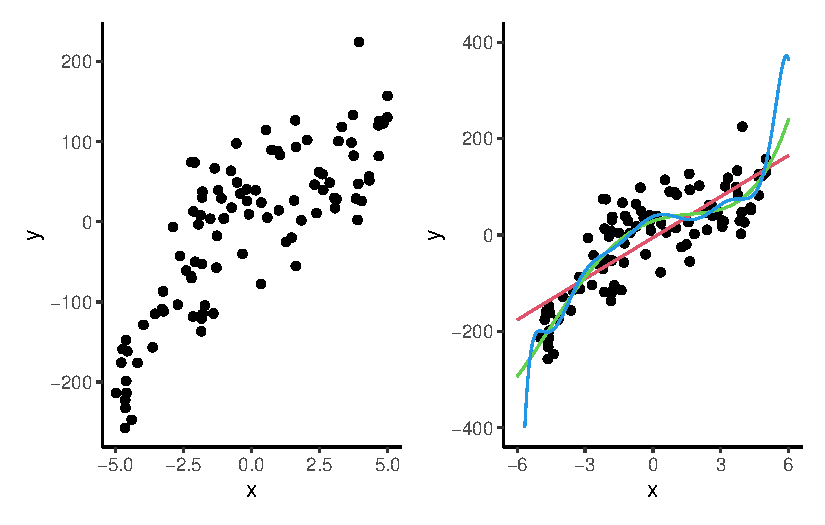
\includegraphics[width=1\textwidth,height=\textheight]{selectionmodeles_files/figure-pdf/fig-donneestest-1.pdf}

}

\caption{\label{fig-donneestest}Nuage de points de 100 observations
simulées d'un modèle polynomial de degré inconnu (gauche) et ajustement
de différents polynômes de degré variable (droite).}

\end{figure}%

Ces données ont été obtenues par simulation et le vrai modèle
sous-jacent (celui qui a généré les données) est le modèle cubique,
c'est-à-dire le modèle d'ordre \(k=3\).

J'ai ajusté tour à tour à tour les modèles polynomiaux jusqu'à l'ordre
10, avec l'échantillon d'apprentissage de taille 100. C'est-à-dire, le
modèle linéaire avec un polynôme d'ordre \(k=1\) (linéaire), \(k=2\)
(quadratique), etc., jusqu'à \(k=10\). J'ai ensuite obtenu la valeur de
l'erreur quadratique moyenne d'apprentissage pour chacun de ces modèles.
En pratique, on ne pourrait pas calculer l'erreur quadratique moyenne de
généralization puisqu'on ne connaît pas le vrai modèle. J'ai fait une
approximation de cette dernière en simulant 100 000 observations du vrai
modèle (\texttt{selection1\_test}), en obtenant la prédiction pour
chacune de ces 100 000 observations en utilisant le modèle d'ordre \(k\)
ajusté sur les données d'apprentissage et en calculant l'erreur
quadratique moyenne par la suite.

\begin{figure}[ht!]

\centering{

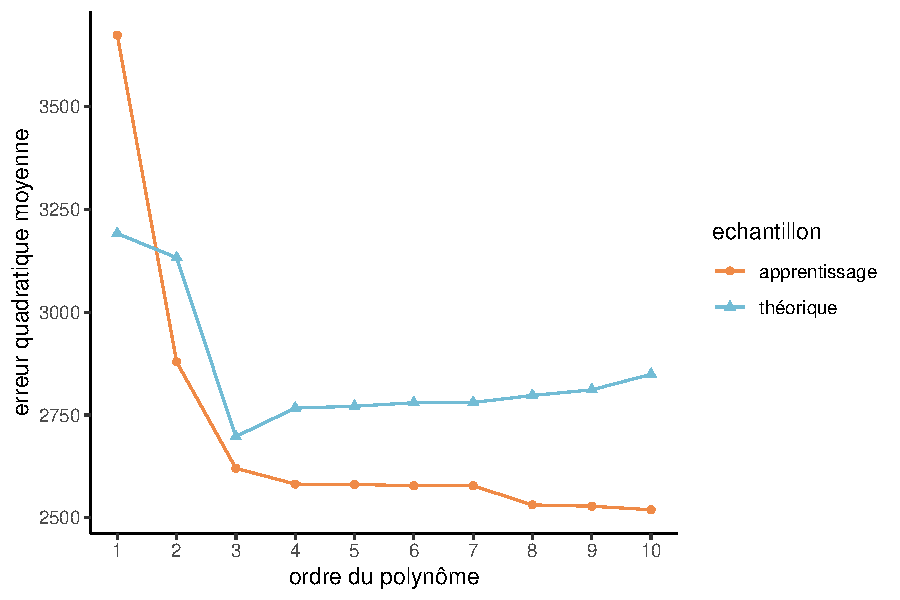
\includegraphics[width=1\textwidth,height=\textheight]{selectionmodeles_files/figure-pdf/fig-plotEQMa-1.pdf}

}

\caption{\label{fig-plotEQMa}erreur quadratique moyenne d'apprentissage
(\(\widehat{\mathsf{EQM}}_a\)) et erreur quadratique moyenne théorique
(\(\mathsf{EQM}\)) en fonction de l'ordre (\(k\)) du polynôme ajusté.}

\end{figure}%

On voit clairement dans la Figure~\ref{fig-plotEQMa} que
l'\(\widehat{\mathsf{EQM}}_a\) diminue en fonction de l'ordre sur
l'échantillon d'apprentissage: plus le modèle est complexe, plus
l'erreur observée sur l'échantillon d'apprentissage est petite. La
courbe \(\mathsf{EQM}\) donne l'heure juste, car il s'agit d'une
estimation de la performance réelle des modèles sur de nouvelles
données. On voit que le meilleur modèle est donc le modèle cubique
(\(k=3\)), ce qui n'est pas surprenant puisqu'il s'agit du modèle que
utilisé pour générer les données. On peut aussi remarquer d'autres
éléments intéressants. Premièrement, on obtient un bon gain en
performance (\(\mathsf{EQM}\)) en passant de l'ordre \(2\) à l'ordre
\(3\). Ensuite, la perte de performance en passant de l'ordre \(3\) à
\(4\), et ensuite à des ordres supérieurs n'est pas si sévère, même si
elle est présente. Cela illustre empiriquement qu'il est préférable
d'avoir un modèle un peu trop complexe que d'avoir un modèle trop
simple. Il serait beaucoup plus grave pour la performance de choisir le
modèle avec \(k=2\) que celui avec \(k=4\).

En pratique par contre, on n'a pas accès à la population : les 100 000
observations qui ont servi à estimer l'\(\mathsf{EQM}\) théorique ne
seront pas disponible. Si on a seulement l'échantillon d'apprentissage,
soit 100 observations dans notre exemple, comment faire alors pour
choisir le bon modèle? C'est ce que nous verrons à partir de la section
suivante.

Mais avant cela, nous allons discuter un peu plus en détail au sujet de
la régression linéaire et d'une mesure très connue, le coefficient de
détermination (\(R^2\)). Supposons que l'on a ajusté un modèle de
régression linéaire \begin{align*}
\widehat{f}(X_1, \ldots, X_p) = \widehat{Y}=\widehat{\beta}_0 + \widehat{\beta}_1X_1+ \cdots + \widehat{\beta}_p X_p.
\end{align*} La somme du carré des erreurs (\(\mathsf{SCE}\)) pour notre
échantillon est \begin{align*}
\mathsf{SCE}=\sum_{i=1}^n (Y_i - \widehat{\beta}_0 - \widehat{\beta}_1X_1 - \cdots - \widehat{\beta}_p X_p)^2 = \sum_{i=1}^n (Y_i-\widehat{Y}_i)^2.
 \end{align*} On peut démontrer que si on ajoute une variable quelconque
au modèle, la valeur de la somme du carré des erreurs va nécessairement
baisser. Il est facile de se convaincre de cela. En régression linéaire,
les estimations sont obtenues par la méthode des moindres carrés qui
consiste justement à minimiser la \(\mathsf{SCE}\). Ainsi, en ajoutant
une variable \(X_{p+1}\) au modèle, la \(\mathsf{SCE}\) ne peut que
baisser car, dans le pire des cas, le paramètre de la nouvelle variable
sera \(\widehat{\beta}_{p+1}=0\) et on retombera sur le modèle sans
cette variable. C'est pourquoi, la quantité
\(\widehat{\mathsf{EQM}}_a=\mathsf{SCE}/n\) ne peut être utilisée comme
outil de sélection de modèles en régression linéaire.

Nous venons d'ailleurs d'illustrer cela avec notre exemple sur les
modèles polynomiaux. En effet, augmenter l'ordre du polynôme de \(1\)
revient à ajouter une variable. Le coefficient de détermination
(\(R^2\)) est souvent utilisé, à tort, comme mesure de qualité du
modèle. Il peut s'interpréter comme étant la proportion de la variance
de \(Y\) qui est expliquée par le modèle.

Le coefficient de détermination est \begin{align*}
R^2=\{\mathsf{cor}(\boldsymbol{y}, \widehat{\boldsymbol{y}})\}^2 = 1-\frac{\mathsf{SCE}}{\mathsf{SCT}},
\end{align*} où \(\mathsf{SCT}=\sum_{i=1}^n (Y_i-\overline{Y})^2\) est
la somme des carrés totale calculée en centrant les observations. La
somme des carrés totale, \(\mathsf{SCT}\), ne varie pas en fonction du
modèle. Ainsi, on voit que le \(R^2\) va méchaniquement augmenter
lorsqu'on ajoute une variable au modèle (car la \(\mathsf{SCE}\)
diminue). C'est pourquoi on ne peut pas l'utiliser comme outil de
sélection de variables.

Le problème principal que nous avons identifié jusqu'à présent afin
d'être en mesure de bien estimer la performance d'un modèle est le
suivant : si on utilise les mêmes observations pour évaluer la
performance d'un modèle que celles qui ont servi à l'ajuster, on va
surestimer sa performance.

Il existe deux grandes approches pour contourner ce problème lorsque le
but est de faire de la sélection de variables ou de modèle :

\begin{itemize}
\tightlist
\item
  utiliser les données de l'échantillon d'apprentissage (en échantillon)
  et pénaliser la mesure d'ajustement (ici \(\widehat{\mathsf{EQM}}_a\))
  pour tenir compte de la complexité du modèle (par exemple, à l'aide de
  critères d'informations).
\item
  tenter d'estimer l'\(\mathsf{EQM}\) directement sur d'autres données
  (hors échantillon) en utilisant des méthodes de rééchantillonnage,
  notamment la validation croisée ou la validation externe (division de
  l'échantillon).
\end{itemize}

\subsection{Pénalisation et critères
d'information}\label{puxe9nalisation-et-crituxe8res-dinformation}

Plaçons-nous dans le contexte de la régression linéaire pour l'instant.
Nous avons déjà utilisé les critères \(\mathsf{AIC}\) et
\(\mathsf{BIC}\) en analyse factorielle. Il s'agit de mesures qui
découlent d'une méthode d'estimation des paramètres, la méthode du
maximum de vraisemblance.

Il s'avère que les estimateurs des paramètres obtenus par la méthode des
moindres carrés en régression linéaire sont équivalents à ceux provenant
de la méthode du maximum de vraisemblance si on suppose la normalité des
termes d'erreurs du modèle. Ainsi, dans ce cas, nous avons accès aux
\(\mathsf{AIC}\) et \(\mathsf{BIC}\), deux critères d'information
définis pour les modèles dont la fonction objective est la vraisemblance
(qui mesure la probabilité des observations sous le modèle postulé
suivant une loi choisie par l'utilisateur). La fonction de vraisemblance
\(\mathcal{L}\) et la log-vraisemblance \(\ell\) mesurent l'adéquation
du modèle.

Supposons que nous avons ajusté un modèle avec \(p\) paramètres en tout
(\textbf{incluant} l'ordonnée à l'origine). En régression linéaire, le
critère d'information d'Akaike, \(\mathsf{AIC}\), est \begin{align*}
\mathsf{AIC} &=-2 \ell(\widehat{\boldsymbol{\beta}}, \widehat{\sigma}^2) +2p = n \ln (\mathsf{EQM}) + 2p + \text{constante},
\end{align*} tandis que le critère d'information bayésien de Schwartz,
\(\mathsf{BIC}\), est défini par \begin{align*}
\mathsf{BIC} &=-2 \ell(\widehat{\boldsymbol{\beta}}, \widehat{\sigma}^2) + p\ln(n)=n \ln (\mathsf{EQM}) + p\ln(n) + \text{constante}.
\end{align*} Plus la valeur du \(\mathsf{AIC}\) (ou du \(\mathsf{BIC}\))
est petite, meilleur est l'adéquation. Que se passe-t-il lorsqu'on
ajoute un paramètre à un modèle? D'une part, la somme du carré des
erreurs va méchaniquement diminuer tout comme l'erreur quadratique
moyenne \(\textsf{EQM} = \textsf{SCE}/n\), donc la quantité
\(n \ln (\mathsf{EQM})\) va diminuer. D'autre part, la valeur de \(p\)
augmente de \(1\). Ainsi, le \(\mathsf{AIC}\) peut soit augmenter, soit
diminuer, lorsqu'on ajoute un paramètre; idem pour le \(\mathsf{BIC}\).
Par exemple, le \(\mathsf{AIC}\) va diminuer seulement si la baisse de
la somme du carré des erreurs est suffisante pour compenser le fait que
le terme \(2p\) augmente à \(2 (p+1)\).

Ces critères pénalisent l'ajout de variables afin de se prémunir contre
le surajustement. De plus, le \(\mathsf{BIC}\) pénalise plus que le
\(\mathsf{AIC}\). Par conséquent, le critère \(\mathsf{BIC}\) va choisir
des modèles contenant soit le même nombre, soit moins de paramètres que
le \(\mathsf{AIC}\).

Les critères \(\mathsf{AIC}\) et \(\mathsf{BIC}\) peuvent être utilisés
comme outils de sélection de variables en régression linéaire mais aussi
beaucoup plus généralement avec d'autres méthodes basées sur la
vraisemblance (analyse factorielle, régression logistique, etc.) En
fait, n'importe quel modèle dont les estimateurs proviennent de la
méthode du maximum de vraisemblance produira ces quantités. Nous
donnerons des formules générales pour le \(\mathsf{AIC}\) et le
\(\mathsf{BIC}\) dans le chapitre sur la régression logistique.

Le critère \(\mathsf{BIC}\) est le seul de ces critères qui est
convergent. Cela veut dire que si l'ensemble des modèles que l'on
considère contient le vrai modèle, alors la probabilité que le critère
\(\mathsf{BIC}\) choisissent le bon modèle tend vers 1 lorsque \(n\)
tend vers l'infini. Il faut mettre cela en perspective : il est peu
vraisemblable que \(Y\) ait été généré exactement selon un modèle de
régression linéaire, car le modèle de régression n'est qu'une
approximation de la réalité. Certains auteurs trouvent que le
\(\mathsf{BIC}\) est quelquefois trop sévère (il choisit des modèles
trop simples) pour les tailles d'échantillons finies. Dans certaines
applications, cette parcimonie est utile, mais il n'est pas possible de
savoir d'avance lequel de ces deux critères (\(\mathsf{AIC}\) et
\(\mathsf{BIC}\)) sera préférable pour un problème donné.

Il est facile d'obtenir le \(\mathsf{AIC}\) et \(\mathsf{BIC}\) avec les
méthodes \texttt{AIC} et \texttt{BIC}. On illustre ceci avec le modèle
cubique:

\begin{Shaded}
\begin{Highlighting}[]
\FunctionTok{data}\NormalTok{(polynome, }\AttributeTok{package =} \StringTok{"hecmulti"}\NormalTok{)}
\CommentTok{\# Ajuster un polynôme de degré trois (modèle cubique)}
\NormalTok{mod\_cub }\OtherTok{\textless{}{-}} \FunctionTok{lm}\NormalTok{(y }\SpecialCharTok{\textasciitilde{}} \FunctionTok{poly}\NormalTok{(x, }\DecValTok{3}\NormalTok{),}
              \AttributeTok{data =}\NormalTok{ polynome)}
\FunctionTok{summary}\NormalTok{(mod\_cub) }\CommentTok{\# Tableau résumé des coefficients}
\FunctionTok{AIC}\NormalTok{(mod\_cub)}
\FunctionTok{BIC}\NormalTok{(mod\_cub)}
\end{Highlighting}
\end{Shaded}

Le Tableau~\ref{tbl-polynome-ajustement} résume ces quantités pour tous
les modèles de l'ordre 1 à l'ordre 10.

\begin{longtable}[]{@{}
  >{\raggedright\arraybackslash}p{(\columnwidth - 12\tabcolsep) * \real{0.0300}}
  >{\raggedleft\arraybackslash}p{(\columnwidth - 12\tabcolsep) * \real{0.1500}}
  >{\raggedleft\arraybackslash}p{(\columnwidth - 12\tabcolsep) * \real{0.2700}}
  >{\raggedleft\arraybackslash}p{(\columnwidth - 12\tabcolsep) * \real{0.0600}}
  >{\raggedleft\arraybackslash}p{(\columnwidth - 12\tabcolsep) * \real{0.1500}}
  >{\raggedleft\arraybackslash}p{(\columnwidth - 12\tabcolsep) * \real{0.1500}}
  >{\raggedleft\arraybackslash}p{(\columnwidth - 12\tabcolsep) * \real{0.1900}}@{}}

\caption{\label{tbl-polynome-ajustement}Mesures de la qualité de
l'ajustement d'un modèle polynomial aux données en fonction de l'ordre
du polynôme.}

\tabularnewline

\toprule\noalign{}
\begin{minipage}[b]{\linewidth}\raggedright
\end{minipage} & \begin{minipage}[b]{\linewidth}\raggedleft
\(\mathsf{EQM}\)
\end{minipage} & \begin{minipage}[b]{\linewidth}\raggedleft
\(\widehat{\mathsf{EQM}}_a\)
\end{minipage} & \begin{minipage}[b]{\linewidth}\raggedleft
\(R^2\)
\end{minipage} & \begin{minipage}[b]{\linewidth}\raggedleft
\(\mathsf{AIC}\)
\end{minipage} & \begin{minipage}[b]{\linewidth}\raggedleft
\(\mathsf{BIC}\)
\end{minipage} & \begin{minipage}[b]{\linewidth}\raggedleft
\(\mathsf{VC}_{10}\)
\end{minipage} \\
\midrule\noalign{}
\endhead
\bottomrule\noalign{}
\endlastfoot
1 & 3191 & 3674 & 0.65 & 1111 & 1119 & 3675 \\
2 & 3133 & 2879 & 0.73 & 1088 & 1099 & 2898 \\
3 & 2697 & 2620 & 0.75 & 1081 & 1094 & 2676 \\
4 & 2767 & 2582 & 0.75 & 1081 & 1097 & 2666 \\
5 & 2771 & 2581 & 0.75 & 1083 & 1102 & 2711 \\
6 & 2780 & 2578 & 0.75 & 1085 & 1106 & 2757 \\
7 & 2780 & 2577 & 0.75 & 1087 & 1111 & 2788 \\
8 & 2797 & 2531 & 0.76 & 1087 & 1113 & 2846 \\
9 & 2811 & 2528 & 0.76 & 1089 & 1118 & 2896 \\
10 & 2849 & 2519 & 0.76 & 1091 & 1122 & 2976 \\

\end{longtable}

\begin{figure}[ht!]

\centering{

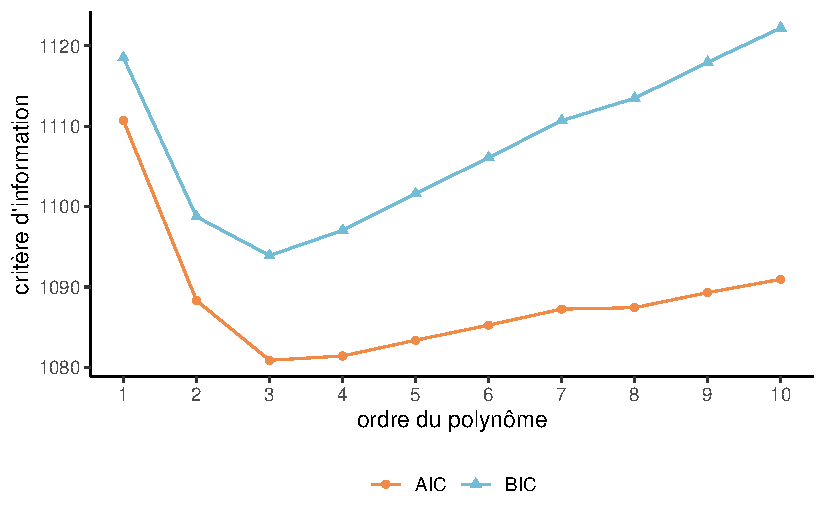
\includegraphics[width=1\textwidth,height=\textheight]{selectionmodeles_files/figure-pdf/fig-polynome-ajustement-1.pdf}

}

\caption{\label{fig-polynome-ajustement}Critères d'information en
fonction de l'ordre du polynôme.}

\end{figure}%

On voit dans le Tableau~\ref{tbl-polynome-ajustement} que l'erreur
quadratique moyenne des données d'apprentissage,
\(\widehat{\mathsf{EQM}}_a\), diminue toujours à mesure qu'on ajoute des
variables (c'est-à-dire, qu'on augmente l'ordre du polynôme); ces
valeurs sont représentées dans la Figure~\ref{fig-plotEQMa}. Les
critères d'information, \(\mathsf{AIC}\) et \(\mathsf{BIC}\), ne sont
pas sur la même échelle, mais le graphique de la
Figure~\ref{fig-polynome-ajustement} illustre un comportement semblable
à la vraie courbe de l'erreur quadratique moyenne théorique et suggèrent
que le meilleur modèle est le modèle cubique (\(k=3\)), c'est-à-dire le
vrai modèle. N'oubliez pas que ces critères sont calculés avec
l'échantillon d'apprentissage (\(n=100\)), mais en pénalisant l'ajout de
variables. On est ainsi en mesure de contrecarrer le problème provenant
du fait qu'on ne peut pas utiliser directement le
\(\widehat{\mathsf{EQM}}_a\).

Le \(\mathsf{AIC}\) et le \(\mathsf{BIC}\) sont des critères très
utilisés et très généraux. Ils sont disponibles dès qu'on utilise la
méthode du maximum de vraisemblance comme méthode d'estimation.

\subsection{Validation externe}\label{validation-externe}

La deuxième grande approche après celle consistant à pénaliser le
\(\widehat{\mathsf{EQM}}_a\) consiste à tenter d'estimer le
\(\mathsf{EQM}\) directement sans utiliser deux fois les mêmes données.
Nous allons voir deux telles méthodes ici, la validation externe
(division de l'échantillon) et la validation croisée
(\emph{cross-validation}).

Ces deux méthodes s'attaquent directement au problème qu'on ne peut
utiliser (sans ajustement) les mêmes données qui ont servi à estimer les
paramètres d'un modèle pour estimer sa performance. Pour ce faire,
l'échantillon de départ est divisé en deux, ou plusieurs parties, qui
vont jouer des rôles différents.

L'idée de la validation externe est simple. Nous avons un échantillon de
taille \(n\) que nous pouvons diviser \emph{au hasard} en deux parties
de tailles respectives \(n_1\) et \(n_2\) (\(n_1+n_2=n\)), soit

\begin{itemize}
\tightlist
\item
  un échantillon d'apprentissage (\emph{training}) de taille \(n_1\) et
\item
  un échantillon de validation (\emph{test}) de taille \(n_2\).
\end{itemize}

L'échantillon d'apprentissage servira à estimer les paramètres du
modèle. L'échantillon de validation servira à estimer la performance
prédictive (par exemple estimer l'\(\mathsf{EQM}\)) du modèle. Comme cet
échantillon n'a pas servi à estimer le modèle lui-même, il est formé de
« nouvelles » observations qui permettent d'évaluer d'une manière
réaliste la performance du modèle. Comme il s'agit de nouvelles
observations, on n'a pas à pénaliser la complexité du modèle et on peut
directement utiliser le critère de performance choisi, par exemple,
l'erreur quadratique moyenne, c'est-à-dire, la moyenne des erreurs au
carré pour l'échantillon de validation. Cette quantité est une
estimation valable de l'\(\mathsf{EQM}\) de ce modèle. On peut faire la
même chose pour tous les modèles en compétition et choisir celui qui a
la meilleure performance sur l'échantillon de validation.

Cette approche possède plusieurs avantages. Elle est facile à implanter.
Elle est encore plus générale que les critères \(\mathsf{AIC}\) et
\(\mathsf{BIC}\). En effet, ces critères découlent de la méthode
d'estimation du maximum de vraisemblance. Plusieurs autres types de
modèles ne sont pas estimés par la méthode du maximum de vraisemblance
(par exemple, les arbres, les forêts aléatoires, les réseaux de
neurones, etc.) La performance de ces modèles peut toujours être estimée
en divisant l'échantillon. Cette méthode peut donc servir à comparer des
modèles de familles différentes. Par exemple, choisit-on un modèle de
régression linéaire, une forêt aléatoire ou bien un réseau de neurones?

Cette approche possède tout de même un désavantage. Elle nécessite une
grande taille d'échantillon au départ. En effet, comme on divise
l'échantillon, on doit en avoir assez pour bien estimer les paramètres
du modèle (l'échantillon d'apprentissage) et assez pour bien estimer sa
performance (l'échantillon de validation).

La méthode consistant à diviser l'échantillon en deux (apprentissage et
validation) afin de sélectionner un modèle est valide. Par contre, si on
veut une estimation sans biais de la performance du modèle choisi (celui
qui est le meilleur sur l'échantillon de validation), on ne peut pas
utiliser directement la valeur observée de l'erreur de ce modèle sur
l'échantillon de validation car elle risque de sous-évaluer l'erreur. En
effet, supposons qu'on a 10 échantillons et qu'on ajuste 10 fois le même
modèle séparément sur les 10 échantillons. Nous aurons alors 10
estimations différentes de l'erreur du modèle. Il est alors évident que
de choisir la plus petite d'entre elles sous-estimerait la vraie erreur
du modèle. C'est un peu ce qui se passe lorsqu'on choisit le modèle qui
minimise l'erreur sur l'échantillon de validation. Le modèle lui-même
est un bon choix, mais l'estimation de son erreur risque d'être
sous-évaluée.

Une manière d'avoir une estimation de l'erreur du modèle retenu consiste
à diviser l'échantillon de départ en trois (plutôt que deux). Aux
échantillons d'apprentissage et de validation, s'ajoute un échantillon «
test ». Cet échantillon est laissé de côté durant tout le processus de
sélection du modèle qui est effectué avec les deux premiers échantillons
tel qu'expliqué plus haut. Une fois un modèle retenu (par exemple celui
qui minimise l'erreur sur l'échantillon de validation), on peut alors
évaluer sa performance sur l'échantillon test qui n'a pas encore été
utilisé jusque là. L'estimation de l'erreur du modèle retenu sera ainsi
valide. Il est évident que pour procéder ainsi, on doit avoir une très
grande taille d'échantillon au départ.

\subsection{Validation croisée}\label{validation-croisuxe9e}

Si la taille d'échantillon n'est pas suffisante pour diviser
l'échantillon en deux et procéder comme nous venons de l'expliquer, la
validation croisée est une bonne alternative. Cette méthode permet
d'imiter le processus de division de l'échantillon.

Voici les étapes à suivre pour faire une validation croisée à \(K\)
groupes (\emph{\(K\)-fold cross-validation}) :

\begin{enumerate}
\def\labelenumi{\arabic{enumi}.}
\tightlist
\item
  Diviser l'échantillon au hasard en \(K\) parties
  \(P_1, P_2, \ldots, P_K\) contenant toutes à peu près le même nombre
  d'observations.
\item
  Pour \(j = 1\) à \(K\),

  \begin{enumerate}
  \def\labelenumii{\roman{enumii}.}
  \tightlist
  \item
    Enlever la partie \(j\).
  \item
    Estimer les paramètres du modèle en utilisant les observations des
    \(K-1\) autres parties combinées.
  \item
    Calculer la mesure de performance (par exemple la somme du carré des
    erreurs) de ce modèle pour le groupe \(P_j\).
  \end{enumerate}
\item
  Combiner les \(K\) estimations de performance pour obtenir une mesure
  de performance finale.\footnote{Le fait d'utiliser \(K \neq n\) mène à
    une estimation biaisée de la quantité d'intérêt et ce biais peut
    être important si \(n\) est petit; un ajustement simple est possible
    pour réduire ce dernier est présenté dans Davison et Hinkley (1997),
    \emph{Bootstrap Methods and their Application}, Cambridge University
    Press à l'équation 6.48.}
\end{enumerate}

Pour l'erreur quadratique moyenne, cette dernière étape revient à
additionner la somme du carré des erreurs avant de diviser par la taille
de l'échantillon totale.

\begin{figure}[ht!]

\centering{

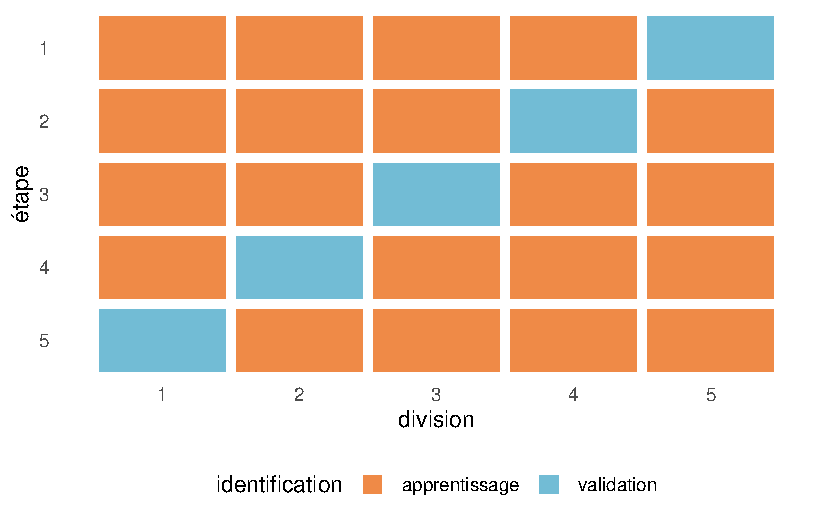
\includegraphics[width=1\textwidth,height=\textheight]{selectionmodeles_files/figure-pdf/fig-validationcroiseeillust-1.pdf}

}

\caption{\label{fig-validationcroiseeillust}Illustration de la
validation croisée: on scinde l'échantillon d'apprentissage en cinq
groupes (abcisse) et à chaque étape, une portion différente des données
est mise de côté et ne sert que pour la validation.}

\end{figure}%

La validation croisée est coûteuse parce qu'on doit ajuster \(K\) fois
le modèles. On recommande habituellement de prendre
\(K=\min\{n^{1/2}, 10\}\) groupes (le choix de cinq ou 10 groupes sont
ceux qui revient le plus souvent en pratique). Si on prend \(K=10\)
groupes, alors chaque modèle est estimé avec 90\% des données et on
prédit ensuite le 10\% restant. Comme on passe en boucle les 10 parties,
chaque observation est prédite une et une seule fois à la fin. Il est
important de souligner que les groupes sont formés de façon aléatoire et
donc que l'estimé que l'on obtient peut être très variable, surtout si
la taille de l'échantillon d'apprentissage est petite. Il arrive
également que le modèle ajusté sur un groupe ne puisse pas être utilisé
pour prédire les observations mises de côté, notamment si des variables
catégorielles sont présentes mais qu'une modalité n'est présente que
dans un des groupes; ce problème se présente en pratique si certaines
classes ont peu d'observations. Un échantillonnage stratifié permet de
pallier à cette lacune et de s'assurer d'une répartition plus homogène
des variables catégorielles.

\begin{Shaded}
\begin{Highlighting}[]
\CommentTok{\# Validation croisée avec k groupes}
\NormalTok{lmkfold }\OtherTok{\textless{}{-}} \ControlFlowTok{function}\NormalTok{(formula, data, k, ...)\{}
   \CommentTok{\# Créer un accumulateur pour le calcul de l\textquotesingle{}EQM}
\NormalTok{   accu }\OtherTok{\textless{}{-}} \DecValTok{0}
\NormalTok{   k }\OtherTok{\textless{}{-}} \FunctionTok{as.integer}\NormalTok{(k) }\CommentTok{\# nombre de groupes}
\NormalTok{   n }\OtherTok{\textless{}{-}} \FunctionTok{nrow}\NormalTok{(data) }\CommentTok{\# nombre d\textquotesingle{}observations}
   \CommentTok{\# Permuter les indices des observatoins}
\NormalTok{   gp }\OtherTok{\textless{}{-}} \FunctionTok{sample.int}\NormalTok{(n, n, }\AttributeTok{replace =} \ConstantTok{FALSE}\NormalTok{)}
   \CommentTok{\# Créer une liste de k éléments avec les nos d\textquotesingle{}observations}
\NormalTok{   folds }\OtherTok{\textless{}{-}} \FunctionTok{split}\NormalTok{(gp, }\FunctionTok{cut}\NormalTok{(}\FunctionTok{seq\_along}\NormalTok{(gp), k, }\AttributeTok{labels =} \ConstantTok{FALSE}\NormalTok{))}
   \ControlFlowTok{for}\NormalTok{(i }\ControlFlowTok{in} \FunctionTok{seq\_len}\NormalTok{(k))\{}
      \CommentTok{\# Extraire les indices des observations de la portion validation}
\NormalTok{      g }\OtherTok{\textless{}{-}} \FunctionTok{as.integer}\NormalTok{(}\FunctionTok{unlist}\NormalTok{(folds[i]))}
      \CommentTok{\# Ajuster le modèles à toutes les données, }
      \CommentTok{\#  moins celles de la portion validation}
\NormalTok{      fitlm }\OtherTok{\textless{}{-}} \FunctionTok{lm}\NormalTok{(formula, }\AttributeTok{data =}\NormalTok{ data[}\SpecialCharTok{{-}}\NormalTok{g,])}
      \CommentTok{\# ajouter l\textquotesingle{}erreur quadratique du pli de validation}
\NormalTok{      accu }\OtherTok{\textless{}{-}}\NormalTok{ accu }\SpecialCharTok{+} 
          \FunctionTok{sum}\NormalTok{((data[g, }\FunctionTok{all.vars}\NormalTok{(formula)[}\DecValTok{1}\NormalTok{]] }\SpecialCharTok{{-}} 
                \FunctionTok{predict}\NormalTok{(fitlm, }\AttributeTok{newdata=}\NormalTok{data[g,]))}\SpecialCharTok{\^{}}\DecValTok{2}\NormalTok{)}
\NormalTok{   \}}
   \CommentTok{\# Diviser par la taille de l\textquotesingle{}échantillon }
   \CommentTok{\# pour obtenir la moyenne}
   \FunctionTok{return}\NormalTok{(accu}\SpecialCharTok{/}\NormalTok{n)}
\NormalTok{\}}

\CommentTok{\# Le paquet \textquotesingle{}caret\textquotesingle{} a une fonction }
\CommentTok{\# pour faire la validation croisée}
\NormalTok{cv\_caret }\OtherTok{\textless{}{-}} 
\NormalTok{  caret}\SpecialCharTok{::}\FunctionTok{train}\NormalTok{(}\AttributeTok{form =}\NormalTok{ formula, }
             \AttributeTok{data =}\NormalTok{ data, }
             \AttributeTok{method =} \StringTok{"lm"}\NormalTok{,}
             \AttributeTok{trControl =}\NormalTok{ caret}\SpecialCharTok{::}\FunctionTok{trainControl}\NormalTok{(}
               \AttributeTok{method =} \StringTok{"cv"}\NormalTok{,}
               \AttributeTok{number =} \DecValTok{10}\NormalTok{))}
\NormalTok{eqm\_cv }\OtherTok{\textless{}{-}}\NormalTok{ cv\_caret}\SpecialCharTok{$}\NormalTok{results}\SpecialCharTok{$}\NormalTok{RMSE}\SpecialCharTok{\^{}}\DecValTok{2}
\end{Highlighting}
\end{Shaded}

Le cas particulier \(K=n\) (en anglais \emph{leave-one-out cross
validation}, ou \(\mathsf{LOOCV}\)) consiste à enlever une seule
observation, à estimer le modèle avec les \(n-1\) autres et à valider à
l'aide de l'observation laissée de côté: on répète cette procédure pour
chaque observation. Pour les modèles linéaires, il existe des formules
explicites qui nous permettent d'éviter d'ajuster \(n\) régressions par
moindre carrés. Cette forme de validation croisée tend à être trop
optimiste.

Il faut garder en tête que le résultat de la validation croisée est
aléatoire parce que la séparation des données en plis l'est également.
La figure Figure~\ref{fig-plotcv}, obtenue en répétant 100 fois la
procédure et en calculant à chaque fois la performance de différents
modèles polynomiaux, montre la variabilité des estimations. Plutôt que
de répéter le calcul, si on a un nombre de groupes \(K\) suffisamment
grand et assez d'observations par pli, on pourrait estimer la
variabilité de la procédure directement. Posons
\(\widehat{\mathsf{EQM}}_{\text{VC}, k}\) (\(k=1, \ldots, K\)) calculer
l'erreur quadratique moyenne de chaque pli. On peut estimer l'écart-type
empirique de cette moyenne via \begin{align*}
\mathsf{sd}(\widehat{\mathsf{EQM}}_{\text{VC}}) = \frac{1}{K-1} \sum_{k=1}^{K} (\widehat{\mathsf{EQM}}_{\text{VC}, k}-\widehat{\mathsf{EQM}}_{\text{VC}})^2.
\end{align*}

Revenons à notre exemple où une seule variable explicative est
disponible et où l'on cherche à déterminer un bon modèle polynomial. La
dernière colonne de Tableau~\ref{tbl-polynome-ajustement},
\(\mathsf{VC}_{10}\), donne les moyennes de 100 réplications de
estimations de l'\(\mathsf{EQM}\) obtenues avec la validation croisée à
10 groupes. Notez que si vous exécutez le programme, vous n'obtiendrez
pas les mêmes valeurs car il y a un élément aléatoire dans ce processus.

Le modèle cubique (ordre 3) est aussi choisi par la validation croisée,
en moyenne (comme il l'était par le \(\mathsf{AIC}\) et le
\(\mathsf{BIC}\)). Le graphe qui suit trace les valeurs de l'estimation
par validation croisée (courbe de validation croisée) et aussi le
\(\mathsf{EQM}\). On voit que l'estimation par validation croisée suit
assez bien la forme du \(\mathsf{EQM}\) (qu'il est supposé estimer).

Pour obtenir la Figure~\ref{fig-plotcv}, j'ai répété 100 fois la
procédure de validation croisée, ce qui me permet d'obtenir 100
estimations pour chaque value de \(k\). Les boîtes à moustache donnent
une idée de la répartition et permettent d'apprécier la variabilité des
estimés de l'erreur quadratique moyenne.

\begin{figure}[ht!]

\centering{

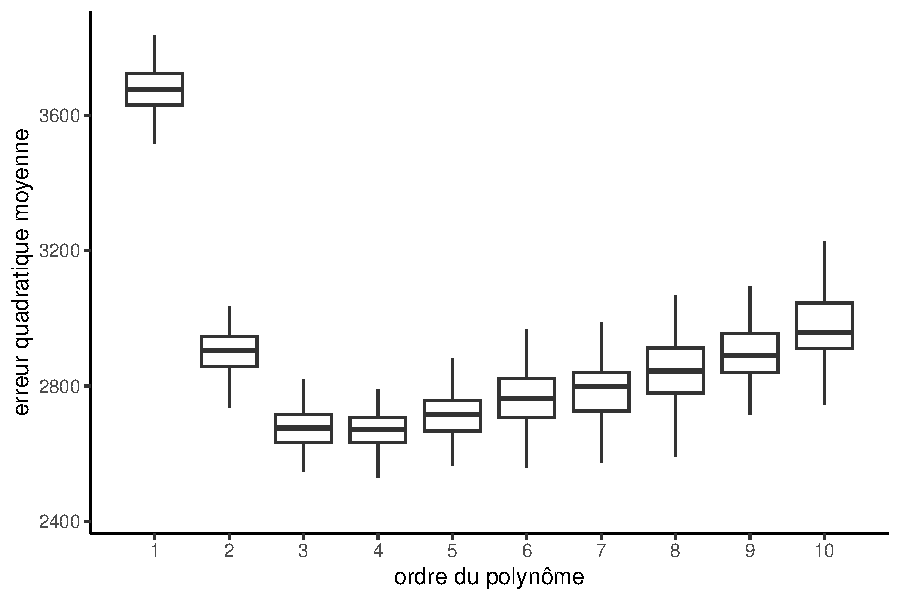
\includegraphics[width=1\textwidth,height=\textheight]{selectionmodeles_files/figure-pdf/fig-plotcv-1.pdf}

}

\caption{\label{fig-plotcv}Boîtes-à-moustaches des 100 réplications des
valeurs de l'erreur quadratique moyenne estimées par validation croisée
à 10 plis pour chaque ordre du polynôme.}

\end{figure}%

Il arrive que la performance soit très similaire pour plusieurs modèles,
auquel cas on pourrait être tenté de prendre le modèle le plus
parsimonieux (c'est-à-dire, celui qui a le moins de paramètres). Si on a
calculé la performance avec la validation croisée et qu'on a obtenu une
mesure d'incertitude pour notre performance, on peut utiliser la règle
du « 1 erreur-type». Cette dernière veut qu'on choisisse le modèle le
plus simple parmi un ensemble
\(\mathcal{M}_0 \subset\cdots \subset \mathcal{M}_m\) qui satisfasse
\begin{align*}
\widehat{\mathsf{EQM}}_{\text{VC}}(\mathcal{M}_i) \leq \min_{m = i+1}^M \widehat{\mathsf{EQM}}_{\text{VC}}(\mathcal{M}_m) + \mathsf{se}\{\widehat{\mathsf{EQM}}_{\text{VC}}(\mathcal{M}_m)\}.
\end{align*} Autrement dit, on trouve le modèle qui minimise notre
critère d'erreur et on choisit ensuite le modèle le plus simple qui soit
à au plus une erreur-type de ce modèle, comme dans la
Figure~\ref{fig-vc-1erreurtype}. On verra ainsi souvent des barres
d'erreurs à \(\pm\) une erreur-type, comme dans la
Figure~\ref{fig-lassopath}.

\begin{figure}[ht!]

\centering{

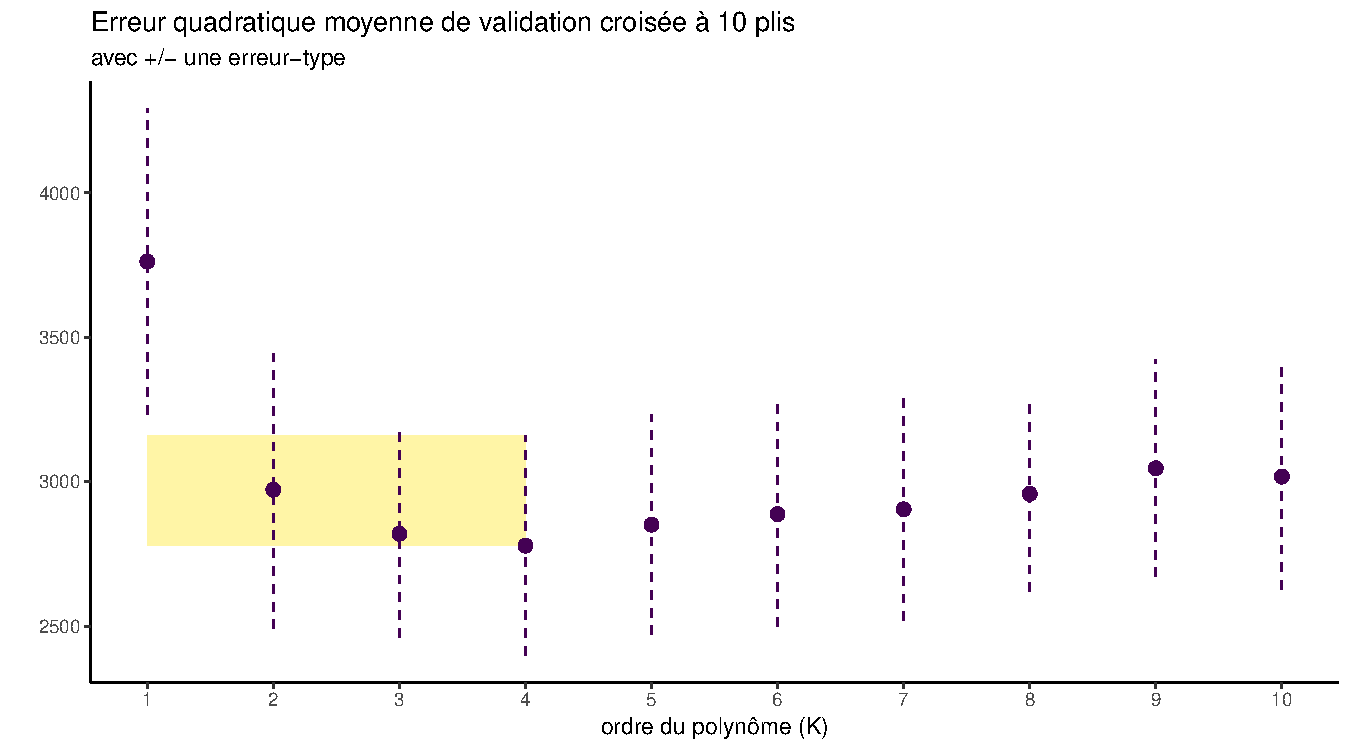
\includegraphics[width=0.85\textwidth,height=\textheight]{figures/fig-validationcroisee-une-erreur-type.pdf}

}

\caption{\label{fig-vc-1erreurtype}Erreur quadratique moyenne estimée
par validation croisée à 10 plis, avec une erreur-type. La bande jaune
indique les valeurs de l'erreur quadratique moyenne à une erreur-type du
modèle qui minimise le critère pour les modèles plus simples.}

\end{figure}%

Pour rappel, le terme écart-type désigne typiquement la variabilité
d'une observation, tandis que l'erreur-type d'une statistique représente
la variabilité de cette quantitée créée en regroupant des observations.
L'erreur-type de la moyenne de \(K\) observations indépendantes qui ont
toutes écart-type \(\sigma\) est ainsi \(\sigma/\sqrt{K}\): c'est
logique puisque la moyenne, basée sur plusieurs observations, est moins
variable qu'une observation.

Ainsi, si on calcule l'écart-type de l'erreur quadratique moyenne d'un
des \(K\) plis avec \(n/K\) observations en moyenne, l'erreur-type de
l'erreur quadratique moyenne globale des \(n\) observations sera
inférieure d'un facteur \(\sqrt{K}\). Si on réplique la validation
croisée plusieurs fois avec des divisions aléatoires différentes,
l'incertitude décroîtra d'autant même si les mesures obtenues ne seront
pas indépendantes puisqu'elles réutilisent les mêmes observations.

Si on veut appliquer la règle d'une , on commence par trouver la modèle
avec la meilleure performance, puis on considère tous les modèles plus
simples (ici avec moins de coefficients, à gauche dans la
Figure~\ref{fig-vc-1erreurtype}). On sélectionne le plus simple parmi
cet ensemble pourvu que son estimation soit dans la bande jaune qui
représente un surenchérissement sur la valeur la plus petite pour
l'erreur quadratique moyenne.

\section{Présentation des données}\label{pruxe9sentation-des-donnuxe9es}

Nous allons présenter un exemple classique de commercialisation de bases
de données qui nous servira à illustrer la sélection de modèles, la
régression logistique et la gestion de données manquantes. Le but est de
cibler les clients pour l'envoi d'un catalogue.

Le contexte est le suivant : une entreprise possède une grande base de
données client. Elle désire envoyer un catalogue à ses clients mais
souhaite maximiser les revenus d'une telle initiative. Il est évidemment
possible d'envoyer le catalogue à tous les clients mais ce n'est
possiblement pas optimal. La stratégie envisagée est la suivante :

\begin{enumerate}
\def\labelenumi{\arabic{enumi}.}
\tightlist
\item
  Envoyer le catalogue à un échantillon de clients et attendre les
  réponses. Le coût de l'envoi d'un catalogue est de 10\$.
\item
  Construire un modèle avec cet échantillon afin de décider à quels
  clients (parmi les autres) le catalogue devrait être envoyé, afin de
  maximiser les revenus.
\end{enumerate}

Plus précisément, on s'intéresse aux clients de 18 ans et plus qui ont
au moins un an d'historique avec l'entreprise et qui ont effectué au
moins un achat au cours de la dernière année. Dans un premier lieu, on a
envoyé le catalogue à un échantillon de 1000 clients. Un modèle sera
construit avec ces 1000 clients afin de cibler lesquels des clients
restants seront choisis pour recevoir le catalogue.

Pour les 1000 clients de l'échantillon d'apprentissage, les deux
variables cibles suivantes sont disponibles :

\begin{itemize}
\tightlist
\item
  \texttt{yachat}, une variable binaire qui indique si le client a
  acheté quelque chose dans le catalogue égale à 1 si oui et 0 sinon.
\item
  \texttt{ymontant}, le montant de l'achat si le client a acheté quelque
  chose.
\end{itemize}

Les 10 variables suivantes sont disponibles pour tous les clients et
serviront de variables explicatives pour les deux variables cibles. Il
s'agit de :

\begin{itemize}
\tightlist
\item
  \texttt{x1}: sexe de l'individu, soit homme (0) ou femme (1);
\item
  \texttt{x2}: l'âge (en année);
\item
  \texttt{x3}: variable catégorielle indiquant le revenu, soit moins de
  35 000\$ (1), entre 35 000\$ et 75 000\$ (2) ou plus de 75 000\$ (3);
\item
  \texttt{x4}: variable catégorielle indiquant la région où habite le
  client (de 1 à 5);
\item
  \texttt{x5}: couple : la personne est elle en couple (0=non, 1=oui);
\item
  \texttt{x6}: nombre d'année depuis que le client est avec la
  compagnie;
\item
  \texttt{x7}: nombre de semaines depuis le dernier achat;
\item
  \texttt{x8}: montant (en dollars) du dernier achat;
\item
  \texttt{x9}: montant total (en dollars) dépensé depuis un an;
\item
  \texttt{x10}: nombre d'achats différents depuis un an.
\end{itemize}

Les données se trouvent dans le fichier \texttt{dbm}. Voici d'abord des
statistiques descriptives pour l'échantillon d'apprentissage.

\begin{Shaded}
\begin{Highlighting}[]
\FunctionTok{data}\NormalTok{(dbm, }\AttributeTok{package =} \StringTok{"hecmulti"}\NormalTok{)}
\FunctionTok{str}\NormalTok{(dbm)}
\CommentTok{\#\textgreater{} tibble [101,000 x 13] (S3: tbl\_df/tbl/data.frame)}
\CommentTok{\#\textgreater{}  $ x1      : int [1:101000] 1 1 0 0 1 1 0 0 0 1 ...}
\CommentTok{\#\textgreater{}  $ x2      : num [1:101000] 42 59 52 32 38 63 35 32 26 32 ...}
\CommentTok{\#\textgreater{}  $ x3      : Factor w/ 3 levels "1","2","3": 1 2 3 1 2 2 2 1 3 1 ...}
\CommentTok{\#\textgreater{}  $ x4      : Factor w/ 5 levels "1","2","3","4",..: 3 3 5 1 5 5 1 3 1 5 ...}
\CommentTok{\#\textgreater{}  $ x5      : int [1:101000] 1 1 1 0 0 1 1 0 0 0 ...}
\CommentTok{\#\textgreater{}  $ x6      : num [1:101000] 8.6 8.6 1.4 10.7 9.1 9.4 10.6 4.8 4 10.3 ...}
\CommentTok{\#\textgreater{}  $ x7      : num [1:101000] 8 9 9 42 5 1 6 5 48 9 ...}
\CommentTok{\#\textgreater{}  $ x8      : num [1:101000] 49 70 120 31 30 28 59 70 73 55 ...}
\CommentTok{\#\textgreater{}  $ x9      : num [1:101000] 159 123 434 110 55 102 593 298 83 90 ...}
\CommentTok{\#\textgreater{}  $ x10     : num [1:101000] 5 5 8 3 3 8 10 6 2 3 ...}
\CommentTok{\#\textgreater{}  $ yachat  : int [1:101000] 0 0 0 0 0 0 0 1 1 1 ...}
\CommentTok{\#\textgreater{}  $ ymontant: num [1:101000] NA NA NA NA NA NA NA 52 79 77 ...}
\CommentTok{\#\textgreater{}  $ test    : Factor w/ 2 levels "0","1": 1 1 1 1 1 1 1 1 1 1 ...}
\end{Highlighting}
\end{Shaded}

\begin{table}

\caption{\label{tbl-contingence-dbm}Tableaux de fréquence pour les
variables catégorielles de la base de données marketing.}

\begin{minipage}{0.25\linewidth}

\begin{longtable}[]{@{}lr@{}}
\toprule\noalign{}
sexe & \(n\) \\
\midrule\noalign{}
\endhead
\bottomrule\noalign{}
\endlastfoot
0 & 534 \\
1 & 466 \\
\end{longtable}

\end{minipage}%
%
\begin{minipage}{0.25\linewidth}

\begin{longtable}[]{@{}lr@{}}
\toprule\noalign{}
revenu & \(n\) \\
\midrule\noalign{}
\endhead
\bottomrule\noalign{}
\endlastfoot
1 & 397 \\
2 & 337 \\
3 & 266 \\
\end{longtable}

\end{minipage}%
%
\begin{minipage}{0.25\linewidth}

\begin{longtable}[]{@{}lr@{}}
\toprule\noalign{}
couple & \(n\) \\
\midrule\noalign{}
\endhead
\bottomrule\noalign{}
\endlastfoot
0 & 575 \\
1 & 425 \\
\end{longtable}

\end{minipage}%
%
\begin{minipage}{0.25\linewidth}

\begin{longtable}[]{@{}lr@{}}
\toprule\noalign{}
région & \(n\) \\
\midrule\noalign{}
\endhead
\bottomrule\noalign{}
\endlastfoot
1 & 216 \\
2 & 185 \\
3 & 216 \\
4 & 191 \\
5 & 192 \\
\end{longtable}

\end{minipage}%

\end{table}%

\begin{figure}[ht!]

\centering{

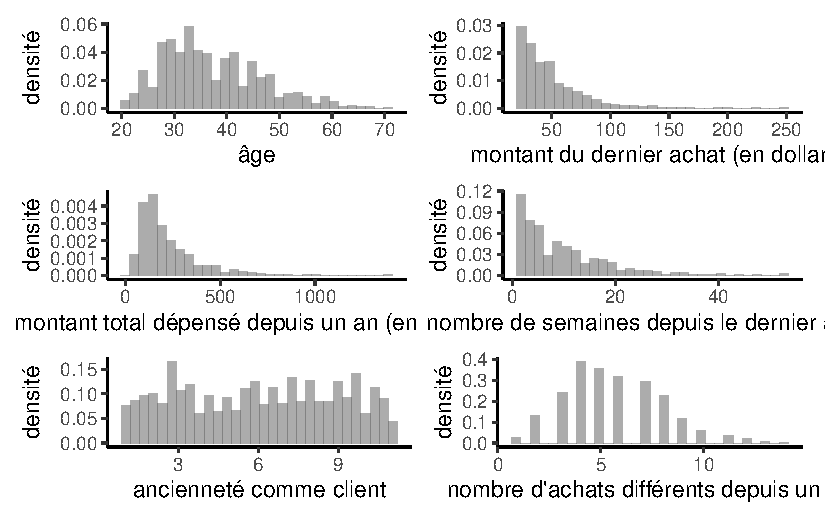
\includegraphics[width=1\textwidth,height=\textheight]{selectionmodeles_files/figure-pdf/fig-histogrammes-eda-dbm-1.pdf}

}

\caption{\label{fig-histogrammes-eda-dbm}Histogrammes des variables
continues de la base de données \texttt{dbm} pour les 1000 clients par
intention d'achat.}

\end{figure}%

Il y a 46.6\% de femmes parmi les 1000 clients de l'échantillon. De
plus, 39.7\% ont un revenu de moins de 35 000\$, 33.7\% sont entre 35
000\$ et 75 000\$ et 26.6\% ont plus de 75 000\$. 42.5\% de ces clients
qui ont un conjoint.

\begin{longtable}[t]{llrrrr}

\caption{\label{tbl-statdescript-dbm}Statistiques descriptives des
variables numériques de la base de données marketing.}

\tabularnewline

\toprule
variable & description & moyenne & écart-type & min & max\\
\midrule
x2 & âge & 37.06 & 9.27 & 20 & 70\\
x6 & nombre d’année comme client & 6.01 & 2.92 & 1 & 11\\
x7 & nombre de semaines depuis le dernier achat & 9.97 & 9.34 & 1 & 52\\
x8 & montant du dernier achat & 48.41 & 28.27 & 20 & 252\\
x9 & montant total dépensé sur un an & 229.27 & 173.97 & 22 & 1407\\
\addlinespace
x10 & nombre d'achats différents sur un an & 5.64 & 2.31 & 1 & 14\\
\bottomrule

\end{longtable}

Le nombre d'achats différents depuis un an par ces clients varie entre 1
et 14. Un peu plus de la moitié (51.4\%) ont fait cinq achats ou moins.
Parmi les 1000 clients de l'échantillon d'apprentissage, 210 ont acheté
quelque chose dans le catalogue. La variable yachat sera l'une des
variables que nous allons chercher à modéliser en vue d'obtenir des
prédictions.

L'âge des 1000 clients de l'échantillon d'apprentissage varie entre 20
et 70 avec une moyenne de 37.1 ans. En moyenne, ces clients ont acheté
pour 229.30\$ depuis un an. Le dernier achat de ces clients remonte, en
moyenne, à 10 semaines.

Dans cette section, nous modéliserons le montant d'achat,
\texttt{ymontant}. Seuls 210 clients ont acheté quelque chose dans le
catalogue et les statistiques rapportées correspondent seulement à ces
derniers, car la variable \texttt{ymontant} est manquante si le client
n'a rien acheté dans le catalogue. On pourrait également remplacer ces
valeurs par des zéros et les modéliser, mais nous aborderons cet aspect
ultérieurement. Les clients qui ont acheté quelque chose ont dépensé en
moyenne 67.3\$, et au minimum 25\$. La
Figure~\ref{fig-histogrammes-eda-dbm} présente les histogrammes de
quelques unes de ces variables.

Il y a plusieurs façons d'utiliser l'échantillon d'apprentissage afin de
mieux cibler les clients à qui envoyer le catalogue et maximiser les
revenus. En voici quelques unes.

\begin{enumerate}
\def\labelenumi{\alph{enumi})}
\tightlist
\item
  On pourrait développer un modèle afin d'estimer la probabilité qu'un
  client achète quelque chose si on lui envoie un catalogue. Plus
  précisément, on peut développer un modèle pour
  \(\Pr(\texttt{yachat}=1)\). Comme la variable \texttt{yachat} est
  binaire, un modèle possible est la régression logistique, que nous
  décrirons au chapitre suivant. Ainsi, en appliquant le modèle aux 100
  000 clients restant, on pourra cibler les clients susceptibles
  d'acheter (ceux avec une probabilité élevée).
\item
  Une autre façon serait de tenter de prévoir le montant d'argent
  dépensé. Nous venons de voir la distribution de la variable
  \texttt{ymontant}. Il y a deux situations, ceux qui ont acheté et ceux
  qui n'ont pas achetés. En conditionnant sur le fait d'avoir acheté
  quelque chose, il est possible de décomposer le problème de la manière
  suivante :
\end{enumerate}

\begin{align*}
\mathsf{E}(\texttt{ymontant}) &= \mathsf{E}(\texttt{ymontant} \mid \texttt{yachat}=1) \mathsf{P}(\texttt{yachat}=1) \\& \quad + 
\mathsf{E}(\texttt{ymontant} \mid \texttt{yachat}=0) \mathsf{P}(\texttt{yachat}=0) \\
 &= \mathsf{E}(\texttt{ymontant} \mid \texttt{yachat}=1) \mathsf{P}(\texttt{yachat}=1),
\end{align*} puisque le terme
\(\mathsf{E}(\texttt{ymontant} \mid \texttt{yachat}=0)\) est zéro: les
gens qui n'ont pas acheté n'ont rien dépensé.

On peut donc estimer
\(\mathsf{E}(\texttt{ymontant} \mid \texttt{yachat}=1)\) et
\(\mathsf{P}(\texttt{yachat}=1)\), pour ensuite les combiner et avoir
une estimation de \(\mathsf{E}(\texttt{ymontant})\). Le développement du
modèle pour \(\mathsf{E}(\texttt{ymontant} \mid \texttt{yachat}=1)\)
peut se faire avec la régression linéaire, en utilisant seulement les
clients qui ont acheté dans l'échantillon d'apprentissage, car
\(\texttt{ymontant}\) est une variable continue dans ce cas. Le
développement du modèle pour \(\mathsf{P}(\texttt{yachat}=1)\) peut se
faire avec la régression logistique, tel que mentionné plus haut, en
utilisant tous les 1000 clients de l'échantillon d'apprentissage. En
fait, nous verrons plus loin qu'il est possible d'estimer conjointement
les deux modèles avec un modèle Tobit. En appliquant le modèle aux 100
000 clients restants, on pourra cibler les clients qui risquent de
dépenser un assez grand montant.

Comme nous n'avons pas encore vu la régression logistique, nous allons
nous limiter à illustrer les méthodes qui restent à voir dans ce
chapitre avec la régression linéaire en cherchant à développer un modèle
pour \(\mathsf{E}(\texttt{ymontant} \mid \texttt{yachat}=1)\), le
montant d'argent dépensé par les clients qui ont acheté quelque chose.

La base de donnée contient deux variables explicatives catégorielles. Il
s'agit de revenu (\texttt{x3}) et région (\texttt{x4}). Il faut coder
d'une manière appropriée afin de pouvoir les incorporer dans les
modèles. La manière habituelle est de créer des variables indicatrices
(binaires) qui indiquent si la variable prend ou non une valeur
particulière dans \textbf{R} est de transformer la variable en facteur
(\texttt{factor}). En général, si une variable catégorielle possède
\(K\) valeurs possibles, il est suffisant de créer \(K-1\) indicatrices,
en laissant une modalité comme référence. Par exemple, pour \texttt{x3},
nous allons créer deux variables,

\begin{itemize}
\tightlist
\item
  \texttt{x31}: variable binaire égale à 1 si \texttt{x3} égale 1 et 0
  sinon,
\item
  \texttt{x32}: variable binaire égale à 1 si \texttt{x3} égale 2 et 0
  sinon.
\end{itemize}

Ainsi, la valeur 3 est celle de référence. Ces deux indicatrices sont
suffisantes pour récupérer toute l'information comme le démontre le
Tableau~\ref{tbl-02-dummy}.

\begin{longtable}[]{@{}ccc@{}}
\caption{Valeur des indicateurs en fonction du niveau de la variable
catégorielle}\label{tbl-02-dummy}\tabularnewline
\toprule\noalign{}
\texttt{x3} & \texttt{x31} & \texttt{x32} \\
\midrule\noalign{}
\endfirsthead
\toprule\noalign{}
\texttt{x3} & \texttt{x31} & \texttt{x32} \\
\midrule\noalign{}
\endhead
\bottomrule\noalign{}
\endlastfoot
1 & 1 & 0 \\
2 & 0 & 1 \\
3 & 0 & 0 \\
\end{longtable}

Il est important de noter que, si le modèle qui inclut toutes les
modalités (ordonnée à l'origine, \texttt{x31} et \texttt{x32}) possibles
ne dépend pas de la catégorie de référence, ce ne sera plus le cas si on
permet lors de la sélection de variables de ne conserver que certains
niveaux de la variable catégorielle. Par exemple, si on inclut
uniquement \texttt{x31} comme variable explicative, l'ordonnée à
l'origine englobera toutes les autres valeurs de \texttt{x3}, à savoir
\(\{2, 3\}\).\footnote{La fonction \texttt{MASS::stepAIC} ne segmente
  pas les variables catégorielles: tous les niveaux sont inclus à la
  fois. La fonction \texttt{leaps::regsubsets} va quant à elle créer des
  indicateurs binaires.}

\begin{tcolorbox}[enhanced jigsaw, bottomrule=.15mm, toptitle=1mm, opacityback=0, title=\textcolor{quarto-callout-tip-color}{\faLightbulb}\hspace{0.5em}{Danger de surajustement avec variables catégorielles}, left=2mm, bottomtitle=1mm, colbacktitle=quarto-callout-tip-color!10!white, colback=white, breakable, toprule=.15mm, coltitle=black, arc=.35mm, opacitybacktitle=0.6, colframe=quarto-callout-tip-color-frame, titlerule=0mm, leftrule=.75mm, rightrule=.15mm]

La principale cause de mauvaise performance est le surajustement
sélectif. Dans l'exemple que l'on considère avec la base de données
marketing, la plupart des modalités des variables catégorielles semblent
à première vues suffisantes pour estimer des coefficients. Si on
s'intéresse par contre aux interactions, on se rendra rapidement compte
qu'il y a trop peu de valeurs pour certaines combinaisons (par exemple,
\texttt{x3*x5}) pour estimer de manière fiable l'effet combiné. Si on a
une valeur aberrante dans un groupe avec de faibles modalités, les
indicateurs donneront systématiquement préférence à l'inclusion d'un
terme pour l'accomoder (au détriment de la généralisation). Cela a pour
effet de fausser la sélection et donner une grande erreur quadratique
moyenne de validation. Si certaines modalités ont des effectifs trop
petits, on peut envisager de les regrouper avec d'autres similaires.

\end{tcolorbox}

\section{Sélection de variables}\label{suxe9lection-de-variables}

\subsection{Recherche exhaustive (meilleurs
sous-ensembles)}\label{recherche-exhaustive-meilleurs-sous-ensembles}

Lorsque nous voulons comparer un petit nombre de modèles, il est
relativement aisé d'obtenir les critères (\(\mathsf{AIC}\),
\(\mathsf{BIC}\) ou autre) pour tous les modèles et de choisir le
meilleur. C'était le cas dans l'exemple du choix de l'ordre du polynôme
où il y avait seulement 10 modèles en compétitions. Mais lorsqu'il y a
plusieurs variables en jeu, le nombre de modèles potentiel augmente très
rapidement.

En fait, supposons qu'on a \(p\) variables distinctes disponibles. Avant
même de considérer les transformations des variables et les interactions
entre elles, il y a déjà trop de modèles possibles. En effet, chaque
variable est soit incluse ou pas (deux possibilités) et donc il y a
\(2^p=2\times 2 \times \cdots \times 2\) (\(p\) fois) modèles en tout à
considérer. Ce nombre augmente très rapidement comme en témoigne le
Tableau~\ref{tbl-02-table3}.

\begin{longtable}[t]{rr}

\caption{\label{tbl-02-table3}Nombres de modèles en fonction du nombre
de paramètres.}

\tabularnewline

\toprule
\$p\$ & nombre de paramètres\\
\midrule
5 & 32\\
10 & 1024\\
15 & 32768\\
20 & 1048576\\
25 & 33554432\\
\addlinespace
30 & 1073741824\\
\bottomrule

\end{longtable}

Ainsi, si le nombre de variables est restreint, il est possible de
comparer tous les modèles potentiels et de choisir le meilleur (selon un
critère). II existe même des algorithmes très efficaces qui permettent
de trouver le meilleur modèle sans devoir examiner tous les modèles
possibles. Le nombre de variables qu'il est possible d'avoir dépend de
la puissance de calcul et augmente d'année en année. Par contre, dans
plusieurs applications, il ne sera pas possible de comparer tous les
modèles et il faudra effectuer une recherche limitée. Faire une
recherche exhaustive parmi tous les modèles possibles s'appelle
sélection de tous les sous-ensembles (\emph{best subsets}).

On veut trouver un bon modèle pour prévoir la valeur de
\texttt{ymontant} des clients qui ont acheté quelque chose. On a vu
qu'il y a 210 clients qui ont acheté dans l'échantillon d'apprentissage.
Nous allons chercher à développer un « bon » modèle avec ces 210
clients. Dans ce premier exemple, nous allons seulement utiliser les 10
variables explicatives de base (14 variables avec les indicatrices).

Pour un nombre de variables fixé, le meilleur modèle selon le \(R^2\)
est aussi le meilleur selon les critères d'information \(\mathsf{AIC}\)
et \(\mathsf{BIC}\), pour ce nombre fixé de variables. Pour vous
convaincre de cette affirmation, fixons le nombre de variables et
restreignons-nous seulement aux modèles avec ce nombre de variables.
Comme \(R^2=1 - \mathsf{SCE}/\mathsf{SCT}\) et que \(\mathsf{SCT}\) est
une constante indépendante du modèle, le modèle avec le plus grand
coefficient de détermination, \(R^2\), est aussi celui avec la plus
petite somme du carré des erreurs (\(\mathsf{SCE}\)). Comme
\(\mathsf{AIC}=n \ln (\mathsf{EQM}) + 2p\), ce sera aussi celui avec le
plus petit \(\mathsf{AIC}\) car la pénalité \(2p\) est la même si on
fixe le nombre de variables; la même remarque est valide pour le
\(\mathsf{BIC}\).

Ainsi, pour trouver le meilleur modèle globalement (sans fixer le nombre
de variables), il suffit de trouver le modèle à \(k\) variables
explicatives ayant le coefficient de détermination le plus élevé pour
tous les nombres de variables fixés et d'ensuite de trouver celui qui
minimise le \(\mathsf{AIC}\) (ou le \(\mathsf{BIC}\)) parmi ces modèles.
Ainsi, le modèle linéaire simple qui a le plus grand \(R^2\) est celui
qui inclut l'indicateur de couple (\texttt{x5}). Le meilleur modèle
(selon le \(R^2\)) parmi tous les modèles avec deux variables est celui
avec \texttt{x5} et \texttt{x6}.

\begin{longtable}[t]{lrr}

\caption{\label{tbl-leaps-simple}Modèle parmi les candidats ayant la
plus grande valeur de coefficient de détermination selon le nombre de
régresseurs, avec valeurs des critères d'informations.}

\tabularnewline

\toprule
variables & BIC & AIC\\
\midrule
x5 & -96 & -103\\
x5 x6 & -196 & -206\\
x31 x5 x6 & -311 & -324\\
x31 x5 x6 x10 & -351 & -368\\
x1 x31 x5 x6 x10 & -369 & -389\\
\addlinespace
x1 x31 x5 x6 x7 x10 & -387 & -411\\
x1 x31 x5 x6 x7 x8 x10 & -392 & -419\\
x1 x31 x44 x5 x6 x7 x8 x10 & -391 & -421\\
x1 x2 x31 x44 x5 x6 x7 x8 x10 & -390 & -424\\
x1 x2 x31 x44 x5 x6 x7 x8 x9 x10 & -387 & -424\\
\addlinespace
x1 x2 x31 x43 x44 x5 x6 x7 x8 x9 x10 & -383 & -423\\
x1 x2 x31 x41 x42 x43 x44 x5 x6 x7 x8 x10 & -378 & -422\\
x1 x2 x31 x41 x42 x43 x44 x5 x6 x7 x8 x9 x10 & -375 & -422\\
\bottomrule

\end{longtable}

Un algorithme par séparation et évaluation permet d'effectuer cette
recherche de manière efficace sans essayer tous les candidats pour ces
sous-ensembles. Dans l'exemple, on voit que le modèle avec les variables
\texttt{x1} \texttt{x2} \texttt{x31} \texttt{x44} \texttt{x5}
\texttt{x6} \texttt{x7} \texttt{x8} \texttt{x9} et \texttt{x10} est
celui qui minimise le \(\mathsf{AIC}\) globalement (\(\mathsf{AIC}\) de
-423.754). Le modèle choisi par le \(\mathsf{BIC}\) contient seulement
sept variables explicatives (plutôt que 10), soit \texttt{x1}
\texttt{x31} \texttt{x5} \texttt{x6} \texttt{x7} \texttt{x8}
\texttt{x10}.

\begin{Shaded}
\begin{Highlighting}[]
\FunctionTok{data}\NormalTok{(dbm, }\AttributeTok{package =} \StringTok{"hecmulti"}\NormalTok{)}
\NormalTok{dbm\_a }\OtherTok{\textless{}{-}}\NormalTok{ dbm }\SpecialCharTok{|\textgreater{}}
\NormalTok{  dplyr}\SpecialCharTok{::}\FunctionTok{filter}\NormalTok{(test }\SpecialCharTok{==} \DecValTok{0}\NormalTok{,}
                \SpecialCharTok{!}\FunctionTok{is.na}\NormalTok{(ymontant))}
\CommentTok{\# Conserver données d\textquotesingle{}entraînement (test == 0)}
\CommentTok{\# des personnes qui ont acheté ymontant \textgreater{} 0}
   
\NormalTok{rec\_ex }\OtherTok{\textless{}{-}}\NormalTok{ leaps}\SpecialCharTok{::}\FunctionTok{regsubsets}\NormalTok{(}
  \AttributeTok{x =}\NormalTok{ ymontant }\SpecialCharTok{\textasciitilde{}}\NormalTok{ x1}\SpecialCharTok{+}\NormalTok{x2}\SpecialCharTok{+}\NormalTok{x3}\SpecialCharTok{+}\NormalTok{x4}\SpecialCharTok{+}\NormalTok{x5}\SpecialCharTok{+}\NormalTok{x6}\SpecialCharTok{+}\NormalTok{x7}\SpecialCharTok{+}\NormalTok{x8}\SpecialCharTok{+}\NormalTok{x9}\SpecialCharTok{+}\NormalTok{x10, }
  \AttributeTok{nvmax =} \DecValTok{13}\NormalTok{L,}
  \AttributeTok{method =} \StringTok{"exhaustive"}\NormalTok{,}
  \AttributeTok{data =}\NormalTok{ dbm\_a)}
\NormalTok{resume\_rec\_ex }\OtherTok{\textless{}{-}} \FunctionTok{summary}\NormalTok{(rec\_ex,}
                         \AttributeTok{matrix.logical =} \ConstantTok{TRUE}\NormalTok{)}
\CommentTok{\# Trouver le modèle avec le plus petit BIC}
\NormalTok{min\_BIC }\OtherTok{\textless{}{-}} \FunctionTok{which.min}\NormalTok{(resume\_rec\_ex}\SpecialCharTok{$}\NormalTok{bic)}
\CommentTok{\# Nom des variables dans le modèle retenu}
\NormalTok{rec\_ex}\SpecialCharTok{$}\NormalTok{xnames[resume\_rec\_ex}\SpecialCharTok{$}\NormalTok{which[min\_BIC,]]}
\CommentTok{\# Coefficients}
\CommentTok{\# coef(rec\_ex, id = min\_BIC)}
\end{Highlighting}
\end{Shaded}

Nous avons seulement inclus les variables de base pour ce premier essai.
Il est possible qu'ajouter des variables supplémentaires améliore la
performance du modèle. Pour cet exemple, nous allons considérer les
variables suivantes\footnote{Pourquoi prendre ces variables en
  particulier? Si on suppose que la vrai moyenne de la variable réponse
  \texttt{ymontant} centrée et réduite est une fonction lisse inconnue
  et qu'on utilise les bonnes variables explicatives centrées, le modèle
  ajusté précédemment capture l'approximation de degré 1 (série de
  Taylor) de la vraie fonction de moyenne, tandis que le modèle avec
  termes quadratiques (incluant les interactions) représente
  l'approximation de degré 2.}:

\begin{itemize}
\tightlist
\item
  les variables continues au carré, comme \(\texttt{age}^2\).
\item
  toutes les interactions d'ordre deux entre les variables de base,
  comme \(\texttt{sexe}\cdot\texttt{age}\).
\end{itemize}

Aux variables de base (10 variables explicatives, mais 14 avec les
indicatrices pour les variables catégorielles), s'ajoutent ainsi 90
autres variables. Il y a donc 104 variables explicatives potentielles si
on inclut les interactions et les termes quadratiques. Notez qu'il y a
des interactions entre chacune des variables indicatrices et chacune des
autres variables, mais il ne sert à rien de calculer une interaction
entre deux indicatrices d'une même variable (car une telle variable est
zéro pour tous les individus). De même, il ne sert à rien de calculer le
carré d'une variable binaire codée \(\{0, 1\}\).

Dans la mesure où on aura un ratio d'environ un paramètre pour deux
observations,Le modèle à 104 variables servira uniquement à illustrer le
surajustement. Pensez à la taille de votre échantillon comme à un budget
et aux paramètres comme à un nombre d'items: plus vous achetez d'items,
moins votre budget est élevé pour chacun et leur qualité en pâtira.
Réalistement, un modèle avec plus d'une vingtaine de variables ici
serait difficilement estimable de manière fiable et l'inclusion
d'interactions et de termes quadratiques sert surtout à augmenter la
flexibilité et les possibilités lors de la sélection de variables.

\begin{Shaded}
\begin{Highlighting}[]
\CommentTok{\# (...)\^{}2 crée toutes les interactions d\textquotesingle{}ordre deux}
\CommentTok{\# I(x\^{}2) permet de créer les termes quadratiques}
\NormalTok{formule }\OtherTok{\textless{}{-}} 
  \FunctionTok{formula}\NormalTok{(ymontant }\SpecialCharTok{\textasciitilde{}} 
\NormalTok{          (x1 }\SpecialCharTok{+}\NormalTok{ x2 }\SpecialCharTok{+}\NormalTok{ x3 }\SpecialCharTok{+}\NormalTok{ x4 }\SpecialCharTok{+}\NormalTok{ x5 }\SpecialCharTok{+} 
\NormalTok{             x6 }\SpecialCharTok{+}\NormalTok{ x7 }\SpecialCharTok{+}\NormalTok{ x8 }\SpecialCharTok{+}\NormalTok{ x9 }\SpecialCharTok{+}\NormalTok{ x10)}\SpecialCharTok{\^{}}\DecValTok{2} \SpecialCharTok{+} 
            \FunctionTok{I}\NormalTok{(x2}\SpecialCharTok{\^{}}\DecValTok{2}\NormalTok{) }\SpecialCharTok{+} \FunctionTok{I}\NormalTok{(x6}\SpecialCharTok{\^{}}\DecValTok{2}\NormalTok{) }\SpecialCharTok{+} \FunctionTok{I}\NormalTok{(x7}\SpecialCharTok{\^{}}\DecValTok{2}\NormalTok{) }\SpecialCharTok{+}
            \FunctionTok{I}\NormalTok{(x8}\SpecialCharTok{\^{}}\DecValTok{2}\NormalTok{) }\SpecialCharTok{+} \FunctionTok{I}\NormalTok{(x9}\SpecialCharTok{\^{}}\DecValTok{2}\NormalTok{) }\SpecialCharTok{+} \FunctionTok{I}\NormalTok{(x10}\SpecialCharTok{\^{}}\DecValTok{2}\NormalTok{))}
\NormalTok{mod\_complet }\OtherTok{\textless{}{-}} \FunctionTok{lm}\NormalTok{(formule, }\AttributeTok{data =}\NormalTok{ dbm\_a)}
\end{Highlighting}
\end{Shaded}

Lancer une sélection exhaustive de tous les sous-modèles avec 104
variables risque de prendre un temps énorme. Que faire alors? Il y a
plusieurs possibilités. Nous pourrions faire une recherche limitée avec
les méthodes que nous allons voir à partir de la section suivante. Nous
pourrions aussi combiner les deux approches. Supposons que notre
ordinateur permet de faire une recherche exhaustive de tous les
sous-modèles avec 40 variables. Nous pourrions alors commencer avec une
recherche limitée pour trouver un sous-ensemble de 40 « bonnes »
variables et faire une recherche exhaustive, mais en se restraignant à
ces 40 variables.

\subsection{Méthodes séquentielles de
sélection}\label{muxe9thodes-suxe9quentielles-de-suxe9lection}

Les méthodes de sélection ascendante, descendante et séquentielle sont
des algorithmes gloutons. Elles ont été développées à une époque où la
puissance de calcul était bien moindre, et où il était impossible de
faire une recherche exhaustive des sous-modèles. La procédure
\texttt{leaps::regsubsets} permet une sélection de modèle avec une
approche séquentielle, ascendante ou descendante en choisissant le
meilleur modèle (côté ajustement) avec \(k\) variables
\((k=1, \ldots, k_{\text{max}})\). La procédure \texttt{MASS::stepAIC}
permet de faire cette sélection en utilisant un critère d'information.

L'idée de la \textbf{sélection ascendante} est d'ajouter à chaque étape
au modèle précédent la variable qui améliore le plus l'ajustement. Le
modèle de départ est celui qui n'inclut que l'ordonnée à l'origine
(aucune variable explicative). À chaque étape, on ajoute la variable qui
améliore le plus le critère d'ajustement jusqu'à ce qu'aucune
amélioration ne soit résultante.

Un algorithme glouton résoud un problème d'optimisation étape par étape:
après \(k\) étapes, le modèle construit par la procédure n'est pas
nécessairement le meilleur modèle (si on essayait toutes les
combinaisons). Si on commence avec \(p\) variables, on regarde \(p\)
choix à la première étape de la procédure ascendante, puis on choisit
nue variable parmi les \(p-1\) restantes à la deuxième étape, etc. La
procédure exhaustive essaiera toutes les \(\binom{p}{2}\) combinaisons
possibles\footnote{En pratique, il existe des algorithmes d'optimisation
  qui permettront de faire cette exploration de manière astucieuse sans
  ajuster les modèles sous-optimaux.}: puisque plus de modèles sont
essayés, la solution finale est nécessairement meilleure côté
performance évaluée sur l'échantillon d'apprentissage.

La \textbf{sélection descendante} est similaire, sauf qu'on part avec le
modèle qui inclut toutes les variables explicatives. À chaque étape, on
retire la variable qui contribue le moins à l'ajustement jusqu'à ce que
le critère d'ajustement ne puisse plus être amélioré ou jusqu'à ce qu'on
recouvre le modèle sans variables explicatives, selon le scénario. C'est
l'inverse de la méthode ascendante: on va tester le retrait de chaque
variable individuellement et retirer celle qui est la moins
significative.

La \textbf{méthode de sélection séquentielle} est un hybride entre les
méthodes de sélection ascendantes et descendante. On débute la recherche
à partir du modèle ne contenant que l'ordonnée à l'origine. À chaque
étape, on fait une étape ascendante suivie de une (ou plusieurs) étapes
descendantes. On continue ainsi tant que le modèle retourné par
l'algorithme n'est pas identique à celui de l'étape précédente
(dépendant de notre critère). Le dernier modèle est celui retenu.

Avec la méthode séquentielle, une fois qu'on entre une variable (étape
ascendante), on fait autant d'étapes descendante afin de retirer toutes
les variables qui satisfont le critère de sortie (il peut ne pas y en
avoir). Une fois cela effectué, on refait une étape ascendante pour voir
si on peut ajouter une nouvelle variable.

Avec la méthode ascendante, une fois qu'une variable est dans le modèle,
elle y reste. Avec la méthode descendante, une fois qu'une variable est
sortie du modèle, elle ne peut plus y entrer. Avec la méthode
séquentielle, une variable peut entrer dans le modèle et sortir plus
tard dans le processus. Par conséquent, parmi les trois, la méthode
séquentielle est généralement préférable aux méthodes ascendante et
descendante, car elle inspecte potentiellement un plus grand nombre de
modèles.

\begin{Shaded}
\begin{Highlighting}[]
\CommentTok{\# Cette procédure séquentielle retourne}
\CommentTok{\# la liste de modèles de 1 variables à}
\CommentTok{\# nvmax variables.}
\NormalTok{rec\_seq }\OtherTok{\textless{}{-}} 
\NormalTok{  leaps}\SpecialCharTok{::}\FunctionTok{regsubsets}\NormalTok{(}
    \AttributeTok{x =}\NormalTok{ formule, }
    \AttributeTok{data =}\NormalTok{ dbm\_a,}
    \AttributeTok{method =} \StringTok{"seqrep"}\NormalTok{, }
    \AttributeTok{nvmax =} \FunctionTok{length}\NormalTok{(}\FunctionTok{coef}\NormalTok{(mod\_complet)))}
\FunctionTok{which.min}\NormalTok{(}\FunctionTok{summary}\NormalTok{(rec\_seq)}\SpecialCharTok{$}\NormalTok{bic)}

\CommentTok{\# Alternative avec procédure séquentielle}
\CommentTok{\# qui utilise le critère AIC pour déterminer }
\CommentTok{\# l\textquotesingle{}inclusion ou l\textquotesingle{}exclusion de variables}
\CommentTok{\# }
\CommentTok{\# Procédure plus longue à rouler}
\CommentTok{\# (car les modèles linéaires sont ajustés)}
\CommentTok{\# }
\CommentTok{\# On ajoute ou retire la variable qui}
\CommentTok{\# améliore le plus le critère de sélection}
\CommentTok{\# à chaque étape.}
\NormalTok{seq\_AIC }\OtherTok{\textless{}{-}}\NormalTok{ MASS}\SpecialCharTok{::}\FunctionTok{stepAIC}\NormalTok{(}
  \FunctionTok{lm}\NormalTok{(ymontant }\SpecialCharTok{\textasciitilde{}} \DecValTok{1}\NormalTok{, }\AttributeTok{data =}\NormalTok{ dbm\_a), }
  \CommentTok{\# modèle initial sans variables explicative}
    \AttributeTok{scope =}\NormalTok{ formule, }\CommentTok{\# modèle maximal possible}
    \AttributeTok{direction =} \StringTok{"both"}\NormalTok{, }\CommentTok{\#séquentielle}
    \AttributeTok{trace =} \ConstantTok{FALSE}\NormalTok{, }\CommentTok{\# ne pas imprimer le suivi}
    \AttributeTok{keep =} \ControlFlowTok{function}\NormalTok{(mod, AIC, ...)\{ }
      \CommentTok{\# autres sorties des modèles à conserver}
      \FunctionTok{list}\NormalTok{(}\AttributeTok{bic =} \FunctionTok{BIC}\NormalTok{(mod), }
           \AttributeTok{coef =} \FunctionTok{coef}\NormalTok{(mod))\},}
    \AttributeTok{k =} \DecValTok{2}\NormalTok{) }\CommentTok{\#}
\CommentTok{\# Remplacer k=2 par k = log(nrow(dbm\_a)) pour BIC}

\CommentTok{\# L\textquotesingle{}historique des étapes est disponible via}
\CommentTok{\# seq\_AIC$anova}
\end{Highlighting}
\end{Shaded}

La procédure exhaustive est préférable aux méthodes séquentielles si le
nombre de variables n'est pas trop élevé. S'il y a trop de variables,
rien ne nous empêche de combiner plusieurs méthodes: on pourrait par
exemple faire une procédure descendante pour ne conserver que 40
variables. En utilisant seulement ce sous-ensemble de variables, on
choisit le meilleur modèle selon le \(\mathsf{AIC}\) ou le
\(\mathsf{BIC}\) en faisant une recherche exhaustive de tous les
sous-modèles. On pourrait également faire une recherche séquentielle
avec le \(\mathsf{AIC}\) et choisir le modèle parmi l'historique avec le
plus petit \(\mathsf{BIC}\).

\begin{figure}[ht!]

\centering{

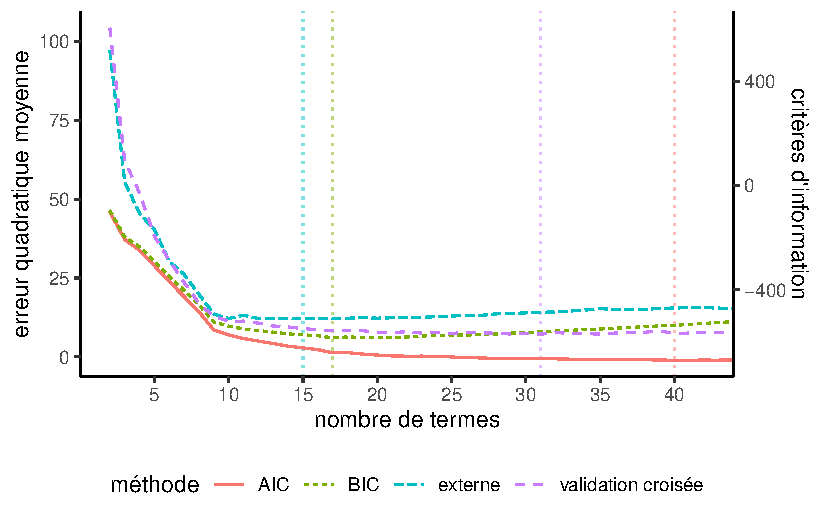
\includegraphics[width=1\textwidth,height=\textheight]{selectionmodeles_files/figure-pdf/fig-perfo-sequentiel-1.pdf}

}

\caption{\label{fig-perfo-sequentiel}Critères d'information et
estimation de l'erreur quadratique moyenne de validation externe et de
validation croisée (10 groupes) pour les 40 premiers modèles de la
procédure descendante, selon le nombre de termes inclus dans la
régression linéaire. Les traitillés verticaux indiquent le nombre de
terme du modèle avec la meilleure valeur du critère pour chaque
méthode.}

\end{figure}%

On peut voir sur la Figure~\ref{fig-perfo-sequentiel} l'historique des
valeurs de AIC et BIC à mesure qu'on augmente le nombre de variables
dans le modèle obtenu par une procédure séquentielle: les mêmes
variables sont enlevées à chaque étape, mais la valeur optimale du
critère est différente pour la sélection finale. Sur l'axe des
abscisses, j'ai ajouté l'erreur quadratique moyenne de l'échantillon de
validation pour les clients avec \texttt{ymontant} positif. Cet exemple
n'est pas réaliste puisqu'on regarde la solution, mais il permet de nous
comparer et de voir à quel point ici le critère d'information bayésien
suit la même tendance que l'erreur quadratique moyenne de validation.
L'erreur quadratique moyenne obtenue par validation croisée est trop
optimiste (mais aléatoire!), comme le AIC. Pour éviter le
surentraînement dans une région où le critère est quasi constant, on
peut utiliser la règle d'une erreur-type. Puisque on a plusieurs
réplications, on peut estimer ce dernier avec la validation croisée en
même temps que l'EQM et choisir le modèle le plus simple à distance une
erreur-type du modèle avec la plus petite erreur de validation croisée.

\subsection{Méthodes de régression avec
régularisation}\label{muxe9thodes-de-ruxe9gression-avec-ruxe9gularisation}

Une façon d'éviter le surajustement est d'ajouter une pénalité sur les
coefficients: ce faisant, on introduit un biais dans nos estimés, mais
dans l'espoir de réduire leur variabilité et ainsi d'obtenir une
meilleur erreur quadratique moyenne.

L'avantage des moindres carrés est que les valeurs ajustées et les
prédictions ne changent pas si on fait une transformation affine (de
type \(Z = aX+b\)). Peu importe le choix d'unité (par exemple, exprimer
une distance en centimètres plutôt qu'en mètres, ou la température en
Farenheit plutôt qu'en Celcius), on obtient le même ajustement. En
revanche, une fois qu'on introduit un terme de pénalité, notre solution
dépendra de l'unité de mesure, d'où l'importance d'utiliser les données
centrées et réduites pour que la solution reste la même.

Les estimateurs des moindres carrés ordinaires pour la régression
linéaire représentent la combinaison qui minimise la somme du carré des
erreurs, \begin{align*}
\mathsf{SCE} = \sum_{i=1}^n \left(y_i - \beta_0 - \sum_{j=1}^pX_{ij}\beta_{j}\right)^2.
\end{align*} On peut ajouter à cette fonction objective \(\mathsf{SCE}\)
un terme additionnel de pénalité qui va contraindre les paramètres à ne
pas être trop grand. On considère une pénalité additionnelle pour la
valeur absolue des coefficients, \begin{align*}
q_1(\lambda) = \lambda \sum_{j=1}^p |\beta_j|.
\end{align*} Pour chaque valeur de \(\lambda\) donnée, on obtiendra une
solution différente pour les estimés car on minimisera désormais
\(\mathsf{SCE} + q_1(\lambda)\). On ne pénalise pas l'ordonnée à
l'origine \(\beta_0\), parce que ce coefficient sert à recentrer les
observations et a une signification particulière: si on standardise les
données, de manière à ce que leur moyenne empirique soit zéro et leur
écart-type un, alors \(\widehat{\beta}_0 = \overline{y}\).

La pénalité \(q_1(\lambda)\) a un rôle particulier parce qu'elle a deux
effets: elle réduit la taille des paramètres, mais elle force également
certains paramètres très proches de zéro à être exactement égaux à zéro,
ce qui fait que la régression pénalité agit également comme outil de
sélection de variables. Des algorithmes efficaces permettent de trouver
la solution du problème d'optimisation \begin{align*}
\min_{\boldsymbol{\beta}} \{\mathsf{SCE} + q_1(\lambda)\} = \min_{\boldsymbol{\beta}}  \left\{\sum_{i=1}^n \left(y_i - \beta_0 - \sum_{j=1}^pX_{ij}\beta_{j}\right)^2 +
\lambda \sum_{j=1}^p |\beta_j|\right\}
\end{align*} laquelle est appelée LASSO. La
Figure~\ref{fig-lassopenalty} montre la fonction objective (lignes de
contour) dans le cas où on a deux paramètres, \(\beta_1\) et
\(\beta_2\): chaque point représente une solution différente au
problème, selon la valeur de la pénalité, allant de la solution des
moindres carrés ordinaires, qui minimisent l'erreur quadratique moyenne,
au centre des ellipses et correspondant à la solution du modèle avec
\(\lambda=0\), à la pénalité infinie qui réduit le modèle à l'ordonnée à
l'origine. À mesure que l'on augmente la pénalité \(\lambda\), les
coefficients rétrécissent vers \((0, 0)\). On peut interpréter la
pénalité \(l_1\) comme une contraire budgétaire: les coefficients
estimés pour une valeur de \(\lambda\) donnée sont ceux qui minimisent
la somme du carré des erreurs, mais doivent être à l'intérieur d'un
budget alloué (losange). La forme de la région fait en sorte que la
solution, qui se trouve sur la bordure du losange, intervient souvent
dans un coin avec certaines coordonnées nulles. Par analogie, pensez à
une course qui démarre à l'origine et dont l'objectif est d'atteindre,
en le moins de temps possible, le point le plus élevé possible. Si le
temps est limité (contrainte due à la pénalité), nous aurons moins de
temps pour parcourir et on coupera au plus court. Sans contrainte de
temps, on peut atteindra le sommet de la montagne correspond à la
solution optimale. Les points représentent le tracé qui permet d'obtenir
le gain en dénivelé le plus rapide, en quelque sorte. Les losanges
représentent la distance maximale qu'on peut parcourir selon la valeur
de \(\lambda\).

\begin{figure}[ht!]

\centering{

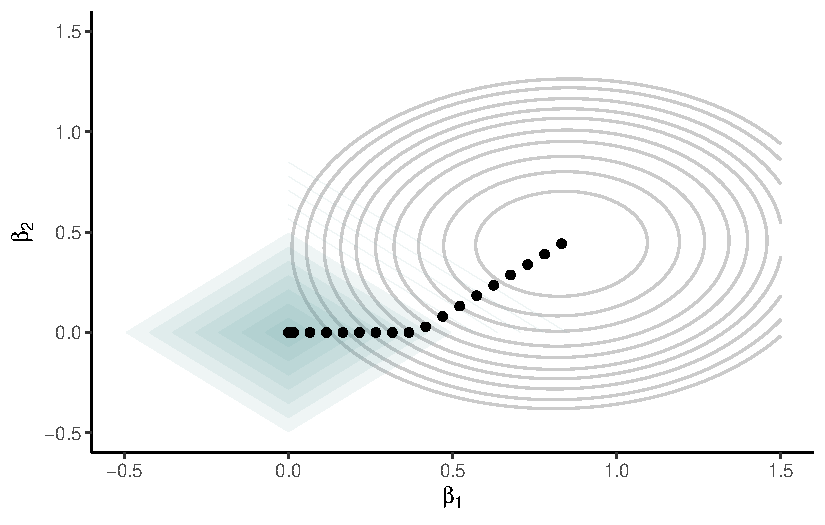
\includegraphics[width=0.85\textwidth,height=\textheight]{selectionmodeles_files/figure-pdf/fig-lassopenalty-1.pdf}

}

\caption{\label{fig-lassopenalty}Courbes de contour du critère de
l'erreur quadratique moyenne (ellipses) et fonction de pénalité
(losanges) pour différentes valeurs de \(\lambda\). Les points dénotent
des solutions différentes et intersectent les contours du losange.}

\end{figure}%

Plusieurs variantes existent dans la littérature qui généralisent le
modèle à des contextes plus compliqués. Le choix des variables à inclure
dans la sélection dépend du choix de la pénalité \(\lambda\), qui est
règle générale estimée par validation croisée à cinq ou 10 groupes.

\begin{Shaded}
\begin{Highlighting}[]
\CommentTok{\# Sélection par LASSO}
\FunctionTok{library}\NormalTok{(glmnet)}
\CommentTok{\# Paramètre de pénalité déterminé par }
\CommentTok{\# validation croisée à partir d\textquotesingle{}un vecteur}
\CommentTok{\# de valeurs candidates}
\NormalTok{lambda\_seq }\OtherTok{\textless{}{-}} \FunctionTok{seq}\NormalTok{(}\AttributeTok{from =} \FloatTok{0.1}\NormalTok{,}
                  \AttributeTok{to =} \DecValTok{10}\NormalTok{, }
                  \AttributeTok{by =} \FloatTok{0.01}\NormalTok{)}
\NormalTok{cv\_output }\OtherTok{\textless{}{-}} 
\NormalTok{  glmnet}\SpecialCharTok{::}\FunctionTok{cv.glmnet}\NormalTok{(}\AttributeTok{x =} \FunctionTok{as.matrix}\NormalTok{(dbm\_a[,}\DecValTok{1}\SpecialCharTok{:}\DecValTok{10}\NormalTok{]), }
            \AttributeTok{y =}\NormalTok{ dbm\_a}\SpecialCharTok{$}\NormalTok{ymontant, }
            \AttributeTok{alpha =} \DecValTok{1}\NormalTok{, }
            \AttributeTok{lambda =}\NormalTok{ lambda\_seq)}
\FunctionTok{plot}\NormalTok{(cv\_output)}

\CommentTok{\# On réestime le modèle avec la pénalité}
\NormalTok{lambopt }\OtherTok{\textless{}{-}}\NormalTok{ cv\_output}\SpecialCharTok{$}\NormalTok{lambda.min }\CommentTok{\# ou lambda.1se}
\NormalTok{lasso\_best }\OtherTok{\textless{}{-}} 
\NormalTok{  glmnet}\SpecialCharTok{::}\FunctionTok{glmnet}\NormalTok{(}
    \AttributeTok{x =} \FunctionTok{as.matrix}\NormalTok{(dbm\_a[,}\DecValTok{1}\SpecialCharTok{:}\DecValTok{10}\NormalTok{]),}
    \AttributeTok{y =}\NormalTok{ dbm\_a}\SpecialCharTok{$}\NormalTok{ymontant,}
    \AttributeTok{alpha =} \DecValTok{1}\NormalTok{, }
    \AttributeTok{lambda =}\NormalTok{ lambopt)}
\CommentTok{\# Prédictions et calcul de l\textquotesingle{}EQM}
\CommentTok{\# On pourrait remplacer \textasciigrave{}newx\textasciigrave{} par }
\CommentTok{\# d\textquotesingle{}autres données (validation externe)}
\NormalTok{pred }\OtherTok{\textless{}{-}} \FunctionTok{predict}\NormalTok{(lasso\_best, }
                \AttributeTok{s =}\NormalTok{ lambopt, }
                \AttributeTok{newx =} \FunctionTok{as.matrix}\NormalTok{(dbm\_a[,}\SpecialCharTok{{-}}\DecValTok{1}\NormalTok{]))}
\NormalTok{eqm\_lasso }\OtherTok{\textless{}{-}} \FunctionTok{mean}\NormalTok{((pred }\SpecialCharTok{{-}}\NormalTok{ dbm\_a}\SpecialCharTok{$}\NormalTok{ymontant)}\SpecialCharTok{\^{}}\DecValTok{2}\NormalTok{)}
\end{Highlighting}
\end{Shaded}

Le graphique de la Figure~\ref{fig-lassopath} montre l'évolution de
l'erreur quadratique moyenne estimée en fonction du logarithme naturel
de la pénalité (axe des abscisses). Pour chaque valeur de la pénalité,
le diagramme donne le nombre de coefficients non-nuls (en haut sur le
graphique) et la valeur estimée par validation croisée à 10 groupes de
l'erreur quadratique moyenne, plus ou moins une erreur-type.
Contrairement aux graphiques précédents, les modèles plus simples
correspondent à des valeurs de pénalité plus élevée (vers la droite sur
le graphique): ainsi, la règle d'une erreur-type revient à prendre un
modèle avec une pénalité plus élevée que le modèle qui minimise l'erreur
quadratique moyenne, donc à diminuer les coefficients et potentiellement
le nombre de coefficients non-nuls.

\begin{figure}[ht!]

\centering{

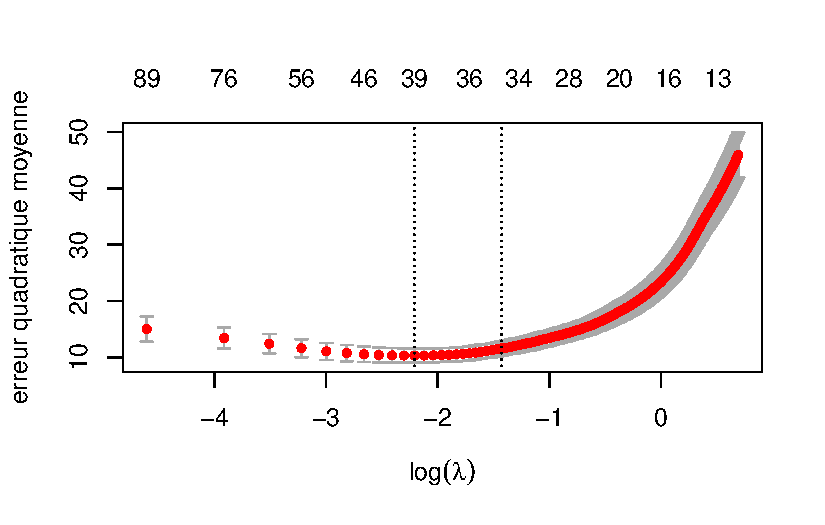
\includegraphics[width=1\textwidth,height=\textheight]{selectionmodeles_files/figure-pdf/fig-lassopath-1.pdf}

}

\caption{\label{fig-lassopath}Estimation de l'erreur quadratique moyenne
(validation croisée à 10 groupes) pour les modèles avec pénalité LASSO
en fonction de la pénalité (échelle log).}

\end{figure}%

\section{Évaluation de la
performance}\label{uxe9valuation-de-la-performance}

La direction de la compagnie a décidé de passer outre vos
recommandations et d'envoyer le catalogue aux 100 000 clients restants;
nous pouvons donc faire un post-mortem afin de voir ce que chaque modèle
aurait donné comme profit, comparativement à la stratégie de référence.
Les 100 000 autres clients serviront d'échantillon de validation pour
évaluer la performance des modèles et, plus précisément, afin d'évaluer
les revenus (ou d'autres mesures de performance) si ces modèles avaient
été utilisés. L'échantillon de validation nous donnera donc l'heure
juste quant aux mérites des différentes approches que nous allons
comparer. En pratique, nous ne pourrions pas faire cela car la valeur de
la variable cible ne serait pas connue pour ces clients et nous
utiliserions plutôt les modèles pour obtenir des prédictions pour
déterminer quels clients cibler avec l'envoi. Parmi, les 100 000 clients
restants, il y en a 23 179 qui auraient acheté quelque chose si on leur
avait envoyé le catalogue. Ces 23 179 observations vont nous servir pour
estimer l'erreur quadratique moyenne (théorique) des modèles retenus par
nos critères.

Commençons par l'estimation de l'erreur quadratique moyenne (moyenne des
carrés des erreurs) pour les deux modèles retenus par le
\(\mathsf{AIC}\) et le \(\mathsf{BIC}\) avec les variables de base. Le
Tableau~\ref{tbl-02-gmse-base} contient aussi l'estimation de l'erreur
quadratique moyenne si on utilise toutes les variables (14 en incluant
les indicatrices) sans faire de sélection. On voit que le modèle choisi
par le \(\mathsf{BIC}\) est le meilleur des trois. Ces deux méthodes
font mieux que le modèle qui inclut toutes les variables sans faire de
sélection, mais nous verrons que leur performance est exécrable: les
variables de base ne permettent pas de capturer les effets présents dans
les données et ce manque de flexibilité coûte cher.

\begin{longtable}[]{@{}
  >{\centering\arraybackslash}p{(\columnwidth - 4\tabcolsep) * \real{0.3158}}
  >{\centering\arraybackslash}p{(\columnwidth - 4\tabcolsep) * \real{0.3684}}
  >{\raggedright\arraybackslash}p{(\columnwidth - 4\tabcolsep) * \real{0.3158}}@{}}
\caption{Estimation de l'erreur quadratique moyenne sur l'échantillon
test avec les variables de base. Les meilleurs modèles selon les
critères d'informations découlent d'une recherche exhaustive de tous les
sous-ensembles.}\label{tbl-02-gmse-base}\tabularnewline
\toprule\noalign{}
\begin{minipage}[b]{\linewidth}\centering
nombre de variables
\end{minipage} & \begin{minipage}[b]{\linewidth}\centering
\(\mathsf{EQM}\)
\end{minipage} & \begin{minipage}[b]{\linewidth}\raggedright
méthode
\end{minipage} \\
\midrule\noalign{}
\endfirsthead
\toprule\noalign{}
\begin{minipage}[b]{\linewidth}\centering
nombre de variables
\end{minipage} & \begin{minipage}[b]{\linewidth}\centering
\(\mathsf{EQM}\)
\end{minipage} & \begin{minipage}[b]{\linewidth}\raggedright
méthode
\end{minipage} \\
\midrule\noalign{}
\endhead
\bottomrule\noalign{}
\endlastfoot
14 & 25.69 & toutes les variables \\
11 & 25.53 & exhaustive - \(\mathsf{AIC}\) \\
9 & 25.04 & exhaustive - \(\mathsf{BIC}\) \\
\end{longtable}

\begin{longtable}[]{@{}ccl@{}}
\caption{Comparaison des méthodes selon l'erreur quadratique moyenne
avec les variables de base, les interactions et les termes
quadratiques.}\label{tbl-02-modelcomparaisonfull}\tabularnewline
\toprule\noalign{}
nombre de variables & \(\mathsf{EQM}\) & méthode \\
\midrule\noalign{}
\endfirsthead
\toprule\noalign{}
nombre de variables & \(\mathsf{EQM}\) & méthode \\
\midrule\noalign{}
\endhead
\bottomrule\noalign{}
\endlastfoot
104 & 19.63 & toutes les variables \\
21 & 12 & séquentielle ascendante, choix selon \(\mathsf{AIC}\) \\
15 & 12.31 & séquentielle ascendante, choix selon \(\mathsf{BIC}\) \\
23 & 12.75 & séquentielle ascendante avec critère \(\mathsf{AIC}\) \\
20 & 12.4 & séquentielle descendante avec critère \(\mathsf{BIC}\) \\
30 & 12 & LASSO, validation croisée avec 10 groupes \\
\end{longtable}

Le Tableau~\ref{tbl-02-modelcomparaisonfull} présente la performance de
toutes les méthodes avec les autres variables. On voit d'abord
qu'utiliser toutes les 104 variables sans faire de sélection fait mieux
(\(\mathsf{EQM}\) de 19.63) que les modèles précédents basés sur les 10
variables originales. Mais faire une sélection permet une amélioration
très importante de la performance (\(\mathsf{EQM}\) jusqu'à 12 dans
l'exemple). Utiliser les 104 variables mène à du surajustement
(\emph{over-fitting}).

Les méthodes séquentielles avec un critère d'information (qui pénalisent
davantage que les tests d'hypothèse classique) mènent à des modèles plus
parcimonieux qui ont une erreur quadratique moyenne de validation plus
faible. Le LASSO performe très bien dans ce cas de figure. Les
coefficients sont tous rétrécis vers zéro (donc le nombre de
coefficients non-nuls n'est pas évocateur), ce qui engendre du biais et
peut affecter négativement la performance si le rapport signal-bruit est
élevé.

Il faut bien comprendre qu'il ne s'agit que d'un seul exemple: il ne
faut surtout pas conclure que la méthode séquentielle sera toujours la
meilleure. En fait, il est impossible de prévoir quelle méthode donnera
les meilleurs résultats.

Il y aurait plusieurs autres approches/combinaisons qui pourraient être
testées. Le but de ce chapitre était simplement de présenter les
principes de base en sélection de modèles et de variables ainsi que
certaines approches pratiques. Il y a d'autres approches intéressantes,
tels le filet élastique. Ces méthodes sont dans la même mouvance moderne
que celle qui consiste à faire la moyenne de plusieurs modèles, en
performant à la fois une sélection de variables et en permettant d'avoir
des parties d'effet par le rétrécissement (\emph{shrinkage}). De récents
développements théoriques permettent aussi de corriger les
valeurs-\emph{p} pour faire de l'inférence post-sélection avec le LASSO.

\begin{tcolorbox}[enhanced jigsaw, bottomrule=.15mm, toptitle=1mm, opacityback=0, title=\textcolor{quarto-callout-note-color}{\faInfo}\hspace{0.5em}{En résumé}, left=2mm, bottomtitle=1mm, colbacktitle=quarto-callout-note-color!10!white, colback=white, breakable, toprule=.15mm, coltitle=black, arc=.35mm, opacitybacktitle=0.6, colframe=quarto-callout-note-color-frame, titlerule=0mm, leftrule=.75mm, rightrule=.15mm]

\begin{itemize}
\tightlist
\item
  En présence de nombreuses variables explicatives, choisir un modèle
  \textbf{prédictif} est compliqué: le nombre de modèles possibles
  augmente rapidement avec le nombre de prédicteurs, \(p\).
\item
  Si un modèle est mal spécifié (variables importantes manquantes),
  alors les estimations sont biaisées. Si le modèle est surspécifié, les
  coefficients correspondants aux variables superflues incluses sont en
  moyenne nuls, mais contribuent à l'augmentation de la variance
  (compromis \emph{biais/variance}).
\item
  La taille du modèle (\(p\), le nombre de variables explicatives) est
  restreinte par le nombre d'observations disponibles, \(n\).

  \begin{itemize}
  \tightlist
  \item
    En général, il faut s'assurer d'avoir suffisamment d'observations
    pour estimer de manière fiable les coefficients (le rapport \(n/p\)
    donne le budget moyen par paramètre).
  \item
    Porter une attention particulière aux variables binaires et aux
    interactions avec ces dernières: si les effectifs de certaines
    modalités sont faibles, il y a possibilité de surajustement.
  \end{itemize}
\item
  Le principal critère pour juger de la qualité d'un modèle linéaire est
  l'erreur quadratique moyenne.

  \begin{itemize}
  \tightlist
  \item
    L'estimation de l'erreur quadratique moyenne obtenue à partir de
    l'échantillon d'apprentissage (qui sert à estimer les paramètres)
    est trompeuse et mène au surajustement:
  \item
    plus le modèle est compliqué, plus cette erreur décroît.
  \item
    cette performance n'est pas répétée sur de nouvelles données.
  \end{itemize}
\item
  Critères de sélection: Plusieurs stratégies existent pour pallier à
  cet excès d'optimisme

  \begin{itemize}
  \tightlist
  \item
    validation externe: diviser le jeu de données aléatoirement au
    préalable en deux ou trois. Nécessite une grande base de données,
    potentiellement sous-optimal.
  \item
    validation croisée: diviser aléatoirement le jeu de données en plis
    et varier les échantillons d'apprentissage en conservant un pli en
    réserve à chaque fois comme validation. Plus coûteux en calcul (il
    faut réajuster plusieurs fois les modèles), applicable avec des
    petites bases de données.
  \item
    pénalisation a posteriori: ajouter une pénalité fonction du nombre
    de paramètres qui compense pour l'augmentation constante de
    l'ajustement (par ex., critères d'information).
  \item
    rétrécissement des coefficients: inclure dans la fonction objective
    qui est maximisée une pénalité qui contraint les paramètres et les
    force à demeurer petit. Cela introduit du biais pour réduire la
    variance.
  \item
    Une pénalité particulière (LASSO) contraint certains paramètres à
    être exactement nuls, ce qui correspond implicitement à une
    sélection de variables.
  \end{itemize}
\item
  En pratique, on cherche à essayer plusieurs modèle pour trouver un
  choix optimal de variables.

  \begin{itemize}
  \tightlist
  \item
    Une recherche exhaustive garantie le survol du plus grand nombre de
    modèles possibles, mais est coûteuse et limitée à moins de 50
    variables.
  \item
    Les algorithmes gloutons de recherche séquentielle sont
    sous-optimaux, mais rapides
  \end{itemize}
\item
  On applique le critère de sélection sur la liste de modèles candidats
  pour retenir celui qui donne la meilleure performance.
\end{itemize}

\end{tcolorbox}

\bookmarksetup{startatroot}

\chapter{Régression logistique}\label{regression-logistique}

\section{Introduction}\label{introduction-1}

En régression linéaire, on cherche à expliquer le comportement d'une
variable quantitative \(Y\) que l'on peut traiter comme étant continue
(elle peut prendre suffisamment de valeurs différentes).

Supposons à présent que l'on veut expliquer le comportement d'une
variable \(Y\) prenant seulement deux valeurs que l'on va noter 0 et 1.

Exemples :

\begin{itemize}
\tightlist
\item
  Est-ce qu'un client potentiel va répondre favorablement à une offre
  promotionnelle?
\item
  Est-ce qu'un client est satisfait du service après-vente?
\item
  Est-ce qu'un client va faire faillite ou non au cours des trois
  prochaines années.
\end{itemize}

En général, on cherchera à expliquer le comportement d'une variable
binaire \(Y\) en utilisant un modèle basé sur \(p\) variables
explicatives \(\mathrm{X}_1, \ldots, \mathrm{X}_p\).

Notre but sera de faire de l'inférence, de la prédiction, ou les deux à
la fois, soit

\begin{enumerate}
\def\labelenumi{\arabic{enumi})}
\tightlist
\item
  \textbf{Inférence} : comprendre comment et dans quelles mesures les
  variables \(\mathbf{X}\) influencent \(Y\) (ou bien la probabilité que
  \(Y=1\)).
\item
  \textbf{Prédiction} : développer un modèle pour prévoir des valeurs de
  \(Y\) futures à partir des variables \(\mathbf{X}\).
\end{enumerate}

\section{Modèle de régression
logistique}\label{moduxe8le-de-ruxe9gression-logistique}

Avec une variable réponse continue, le modèle de régression linéaire,
\begin{align*}
 Y = \beta_0 + \beta_1\mathrm{X}_1 + \cdots + \beta_p \mathrm{X}_p + \varepsilon,
\end{align*} avec \(\mathsf{E}(\varepsilon \mid \mathbf{X})=0\) et
\(\mathsf{Va}(\varepsilon \mid \mathbf{X})=\sigma^2\), peut être écrit
de manière équivalente comme
\(\mathsf{E}(Y  \mid \mathbf{X}) = \beta_0 + \beta_1\mathrm{X}_1 + \cdots + \beta_p\mathrm{X}_p\)
et \(\mathsf{Va}(Y \mid \mathbf{X})=\sigma^2.\)

Si \(Y\) est binaire (0/1), on peut facilement vérifier que
\begin{align*}
\mathsf{E}(Y \mid \mathbf{X}) = \Pr(Y=1 \mid  \mathbf{X}),
\end{align*} soit la probabilité que \(Y\) égale 1 étant donné les
valeurs des variables explicatives. Pour simplifier la notation, posons
la probabilité de succès \(p = \Pr(Y=1 \mid   \mathbf{X})\) en se
rappelant que \(p\) est une fonction des variables explicatives.

À première vue, on peut se demander pourquoi ne pas utiliser le même
modèle que la régression linéaire, c'est-à-dire \begin{align*}
\eta=\beta_0 + \beta_1\mathrm{X}_1 + \cdots + \beta_p \mathrm{X}_p.
\end{align*}

\begin{figure}[ht!]

\centering{

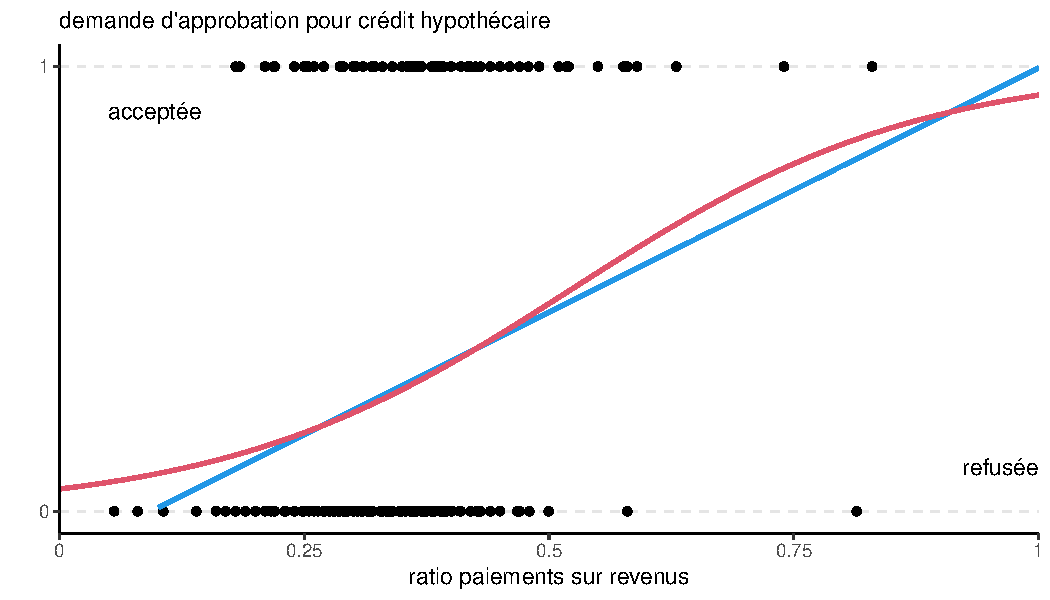
\includegraphics[width=0.8\textwidth,height=\textheight]{reglogistique_files/figure-pdf/fig-demandecredit-1.pdf}

}

\caption{\label{fig-demandecredit}Données de la réserve de Boston sur
l'approbation de prêts hypothécaires (1990); données tirées de Stock et
Watson (2007).}

\end{figure}%

La Figure~\ref{fig-demandecredit} montre le modèle de régression
linéaire (bleu) et le modèle logistique. La pente pour la ligne bleu
correspond à l'augmentation (réputée constante) de la probabilité
d'approbation de crédit, de l'ordre de 11\% par augmentation de 0.1 du
rapport paiements hypothécaires sur revenu.

Il y a quelques problèmes avec le modèle linéaire. D'abord, les données
binaires ne respectent pas le postulat d'égalité des variances, ce qui
rend les tests d'hypothèses caducs. Le problème principal est que \(p\)
est une probabilité. Par conséquent \(p\) prend seulement des valeurs
entre 0 et 1 alors que rien n'empêche \(\eta\) de prendre des valeurs
dans \(\mathbb{R}=(-\infty, \infty)\): par exemple, on voit que la
droite de la Figure~\ref{fig-demandecredit} retourne des prédictions
négatives dès que le ratio paiements/revenus est en dessous de 0.094: on
peut évidemment tronquer ces prédictions à zéro, mais cela sous-tend que
la probabilité d'acceptation est nulle, alors que certaines personnes
dans l'échantillon ont reçu un prêt.

Une façon de résoudre ce problème consiste à appliquer une
transformation à \(p\) de telle sorte que la quantité transformée puisse
prendre toutes les valeurs entre \(-\infty\) et \(\infty\). Le modèle de
régression logistique est défini à l'aide de la transformation
\(\textrm{logit}\), \begin{align*}
\textrm{logit}(p) = \ln\left( \frac{p}{1-p}\right)=\eta=\beta_0 + \beta_1\mathrm{X}_1 + \cdots + \beta_p \mathrm{X}_p,
\end{align*} où \(\ln\) est le logarithme naturel.

En régression linéaire, on suppose que l'espérance de \(Y\) étant donné
les valeurs des variables explicatives est une combinaison linéaire de
ces dernières. En régression logistique, on suppose que le logit de la
probabilité de succès est une combinaison linéaire des variables
explicatives.

Une simple manipulation algébrique permet d'exprimer ce modèle en terme
de la probabilité \(p\), \begin{align*}
 p &= \textrm{expit}(\eta) = \frac{\exp(\eta)}{1+\exp(\eta)}
= \frac{1}{1+\exp(-\eta)}.
\end{align*} On peut voir qu'à mesure que le prédicteur linéaire
\(\eta=\beta_0+\beta_1\mathrm{X}_1 + \cdots + \beta_p\mathrm{X}_p\)
augmente, la probabilité augmente. Si le coefficient \(\beta_j\) est
négatif, \(p\) diminuera à mesure que \(\mathrm{X}_j\) augmente.

\begin{figure}[ht!]

\centering{

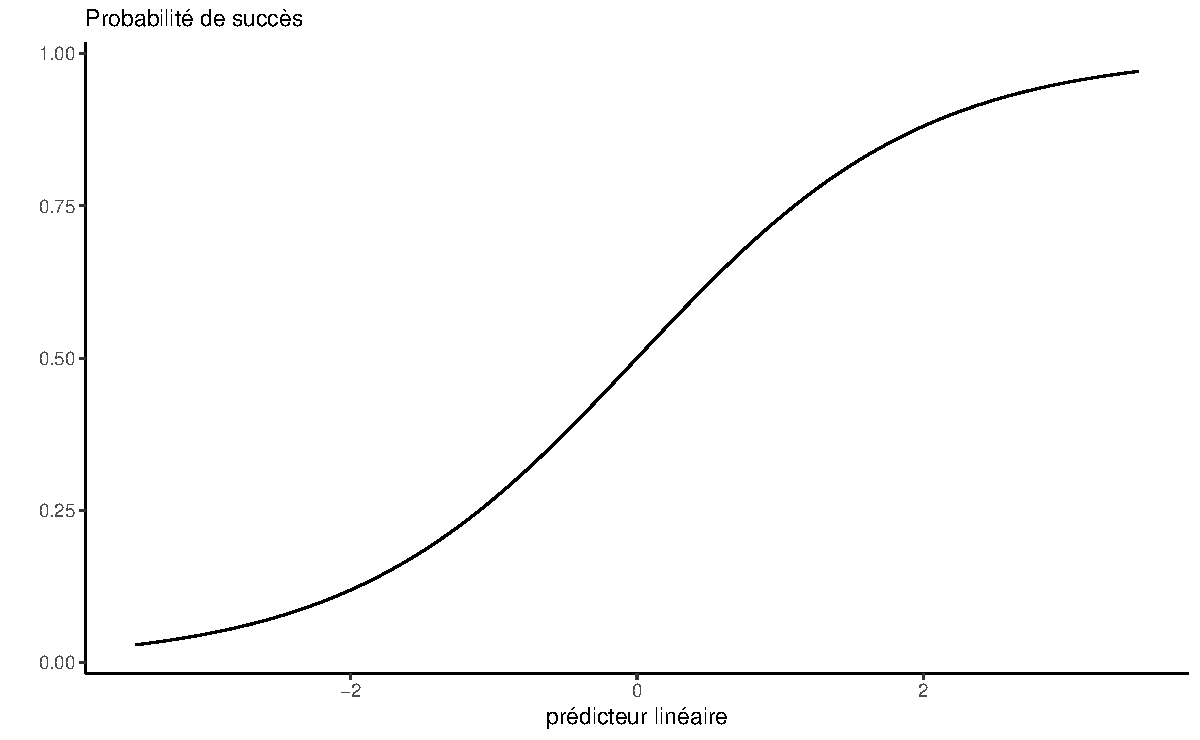
\includegraphics[width=0.8\textwidth,height=\textheight]{reglogistique_files/figure-pdf/fig-logitplot-1.pdf}

}

\caption{\label{fig-logitplot}Valeurs ajustées du modèle de régression
logistique en fonction du prédicteur linéaire \(\eta\).}

\end{figure}%

Pour une variable binaire \(Y\), le rapport \(p/(1-p)\) est appelé
\textbf{cote} et représente le ratio de la probabilité de succès
(\(Y=1\)) sur la probabilité d'échec (\(Y=0\)), \begin{align*}
 \mathsf{cote}(p) = \frac{p}{1-p} = \frac{\Pr(Y=1 \mid \mathbf{X})}{\Pr(Y=0 \mid \mathbf{X})}.
\end{align*}

Par exemple, une cote de 4 veut dire qu'il y a 4 fois plus de chance que
\(Y\) soit égale à \(1\) par rapport à \(0\). Une cote de 0.25 veut dire
le contraire, il y a 4 fois moins de chance que \(Y=1\) par rapport à
\(0\) ou bien, de manière équivalente, il y a 4 fois plus de chance que
\(Y=0\) par rapport à \(1\). Le Tableau~\ref{tbl-cotes} donne un aperçu
de cotes pour quelques probabilités \(p\).

\begin{longtable}[]{@{}
  >{\raggedright\arraybackslash}p{(\columnwidth - 18\tabcolsep) * \real{0.0948}}
  >{\centering\arraybackslash}p{(\columnwidth - 18\tabcolsep) * \real{0.1293}}
  >{\centering\arraybackslash}p{(\columnwidth - 18\tabcolsep) * \real{0.1293}}
  >{\centering\arraybackslash}p{(\columnwidth - 18\tabcolsep) * \real{0.1293}}
  >{\centering\arraybackslash}p{(\columnwidth - 18\tabcolsep) * \real{0.1293}}
  >{\centering\arraybackslash}p{(\columnwidth - 18\tabcolsep) * \real{0.0431}}
  >{\centering\arraybackslash}p{(\columnwidth - 18\tabcolsep) * \real{0.1293}}
  >{\centering\arraybackslash}p{(\columnwidth - 18\tabcolsep) * \real{0.1293}}
  >{\centering\arraybackslash}p{(\columnwidth - 18\tabcolsep) * \real{0.0431}}
  >{\centering\arraybackslash}p{(\columnwidth - 18\tabcolsep) * \real{0.0431}}@{}}

\caption{\label{tbl-cotes}Cote et probabilité de succès}

\tabularnewline

\toprule\noalign{}
\begin{minipage}[b]{\linewidth}\raggedright
\(\Pr(Y=1)\)
\end{minipage} & \begin{minipage}[b]{\linewidth}\centering
0.1
\end{minipage} & \begin{minipage}[b]{\linewidth}\centering
0.2
\end{minipage} & \begin{minipage}[b]{\linewidth}\centering
0.3
\end{minipage} & \begin{minipage}[b]{\linewidth}\centering
0.4
\end{minipage} & \begin{minipage}[b]{\linewidth}\centering
0.5
\end{minipage} & \begin{minipage}[b]{\linewidth}\centering
0.6
\end{minipage} & \begin{minipage}[b]{\linewidth}\centering
0.7
\end{minipage} & \begin{minipage}[b]{\linewidth}\centering
0.8
\end{minipage} & \begin{minipage}[b]{\linewidth}\centering
0.9
\end{minipage} \\
\midrule\noalign{}
\endhead
\bottomrule\noalign{}
\endlastfoot
cote & 0.11 & 0.25 & 0.43 & 0.67 & 1 & 1.5 & 2.3 & 4 & 9 \\
& \(\frac{1}{9}\) & \(\frac{1}{4}\) & \(\frac{3}{7}\) & \(\frac{2}{3}\)
& \(1\) & \(\frac{3}{2}\) & \(\frac{7}{3}\) & \(4\) & \(9\) \\

\end{longtable}

\subsection{Estimation et interprétation des
paramètres}\label{estimation-et-interpruxe9tation-des-paramuxe8tres}

Supposons qu'on dispose d'un échantillon de taille \(n\) sur les
variables \((Y, \mathrm{X}_1, \ldots, \mathrm{X}_p)\). À l'aide de ces
observations, on peut estimer les paramètres
\(\boldsymbol{\beta} = (\beta_0, \beta_1 ,\ldots, \beta_p)\) du modèle
de régression logistique \begin{align*}
\textrm{logit}(p) = \ln \left( \frac{p}{1-p}\right) = \beta_0 + \beta_1 \mathrm{X}_1 + \cdots + \beta_p\mathrm{X}_p.
\end{align*} On obtient ainsi les estimés des paramètres
\(\widehat{\boldsymbol{\beta}}\), desquels découle une estimation de
\(\Pr(Y=1)\) pour les valeurs
\(\mathrm{X}_1=x_1, \ldots, \mathrm{X}_p=x_p\) d'un individu donné,
\begin{align*}
 \widehat{p} = \textrm{expit}(\widehat{\beta}_0 + \cdots + \widehat{\beta}_p\mathrm{X}_p).
\end{align*}

Un modèle ajusté peut ensuite être utilisé pour faire de la
classification (prédiction) pour de nouveaux individus pour lesquels la
variable réponse \(Y\) n'est pas observée. Pour ce faire, on choisit un
point de coupure \(c\) (souvent \(c=0.5\) mais pas toujours) et on
classifie les observations en deux groupes:

\begin{itemize}
\tightlist
\item
  Si \(\widehat{p}< c\), alors \(\widehat{Y}=0\) (c'est-à-dire, on
  assigne cette observation à la catégorie 0 ou échec).
\item
  Si \(\widehat{p} \geq c\), alors \(\widehat{Y}=1\) (c'est-à-dire, on
  assigne cette observation à la catégorie 1 ou succès).
\end{itemize}

On reviendra en détail sur cet aspect dans une section suivante.

La méthode d'estimation des paramètres usuelle est la méthode du maximum
de vraisemblance. Pour les applications, il est suffisant de savoir
manipuler trois quantités importantes: la log-vraisemblance, le
\(\mathsf{AIC}\) et le \(\mathsf{BIC}\). Les deux critères
d'information, que nous avons couvert dans les chapitres précédents,
servent à la sélection de modèles tandis que la log-vraisemblance
\(\ell\) servira à construire un test d'hypothèse.

\subsection{Méthode du maximum de
vraisemblance}\label{muxe9thode-du-maximum-de-vraisemblance}

Cette sous-section est facultative. Elle donne plus de détails sur la
méthode du maximum de vraisemblance et les quantités en découlant, soit
\(\mathsf{AIC}\), \(\mathsf{BIC}\) et
\(\ell(\widehat{\boldsymbol{\beta}})\).

La méthode du maximum de vraisemblance (\emph{maximum likelihood}) est
possiblement la méthode d'estimation la plus utilisée en statistique. En
général, pour un échantillon donné et un modèle avec des paramètres
inconnus \(\boldsymbol{\theta}\), on peut calculer la « probabilité »
d'avoir obtenu les observations de notre échantillon selon les
paramètre. Si on traite cette « probabilité » comme étant une fonction
des paramètres du modèle, \(\boldsymbol{\theta}\), on l'appelle alors la
vraisemblance (\emph{likelihood}). La méthode du maximum de
vraisemblance consiste à trouver les valeurs des paramètres qui
maximisent la vraisemblance. On cherche donc les estimations qui sont
les plus vraisemblables étant donné nos observations.

En pratique, il est habituellement plus simple de chercher à maximiser
le log de la vraisemblance (ce qui revient au même car le logarithme
naturel est une fonction croissante) et on nomme cette fonction la
log-vraisemblance (\emph{log-likelihood}).

Vous connaissez déjà des exemples d'estimateurs du maximum de
vraisemblance. La moyenne d'un échantillon est l'estimateur du maximum
de vraisemblance pour la moyenne de la population \(\mu\) si les
observations représentent un échantillon aléatoire simple tiré d'une loi
normale.

Dans le cas d'un modèle de régression linéaire multiple de la forme
\(Y_i \sim \mathsf{No}(\beta_0 + \sum_{j=1}^p \beta_j\mathrm{X}_{ij}, \sigma^2)\)
des termes indépendants et de même loi, la log-vraisemblance du modèle
pour un échantillon de taille \(n\) est \begin{align*}
 \ell(\boldsymbol{\beta}, \sigma^2) =- \frac{n}{2} \ln(2\pi\sigma^2) - \frac{1}{2\sigma^2}\sum_{i=1}^n (Y_i- \beta_0 - \beta_1 \mathrm{X}_{1i} - \cdots - \beta_p\mathrm{X}_{ip})^2.
\end{align*} Puisque le premier terme ne dépend pas des paramètres
\(\boldsymbol{\beta}\), il est clair que maximiser cette fonction de
\(\boldsymbol{\beta}\) revient à minimiser
\(\sum_{i=1}^n (Y_i- \beta_0 - \beta_1 \mathrm{X}_{1i} - \cdots - \beta_p\mathrm{X}_{ip})^2\):
ce critère est exactement le même que celui des moindres carrés. Par
conséquent, les estimations des paramètres \(\boldsymbol{\beta}\)
provenant de la méthode des moindres carrés peuvent être vues comme
étant des estimateurs du maximum de vraisemblance sous l'hypothèse de
normalité et d'homoscédasticité des observations; il est même possible
d'obtenir une formule explicite pour le calcul dest estimateurs.

Dans le cas de la régression logistique, la fonction de
log-vraisemblance s'écrit \begin{align*}
 \ell(\boldsymbol{\beta}) &= \sum_{i=1}^n Y_i ( \beta_0 + \beta_1 \mathrm{X}_{i1} + \cdots + \beta_p \mathrm{X}_{ip}) \\&- \sum_{i=1}^n \ln\left\{1+\exp(\beta_0 + \cdots + \beta_p\mathrm{X}_{ip})\right\}
\end{align*}

Contrairement au cas de la régression linéaire, on ne peut trouver une
solution explicite pour les valeurs des paramètres qui maximisent cette
fonction. Des méthodes numériques doivent être utilisées pour
l'optimisation. Une fois la maximisation accomplie, on obtient les
estimés du maximum de vraisemblance, \(\widehat{\boldsymbol{\beta}}\).
On peut alors calculer la valeur maximale (numérique) de la
log-vraisemblance, \(\ell(\widehat{\boldsymbol{\beta}})\). Par analogie
avec la régression linéaire la valeur de la log-vraisemblance évaluée à
\(\widehat{\boldsymbol{\beta}}\),
\(\ell(\widehat{\boldsymbol{\beta}})\), augmente toujours lorsqu'on
ajoute des régresseurs et c'est pourquoi on ne pourra pas l'utiliser
comme outil de sélection de variables.

Les critères d'information sont des fonctions de la log-vraisemblance,
mais incluent une pénalité pour le nombre de coefficients
\(\boldsymbol{\beta}\), \begin{align*}
 \mathsf{AIC} & = -2 \ell(\widehat{\boldsymbol{\beta}}) + 2(p+1)\\
 \mathsf{BIC} & = -2 \ell(\widehat{\boldsymbol{\beta}}) + \ln(n)(p+1)
\end{align*}

Ces définitions sont utilisables dans plusieurs situations lorsque le
modèle est ajusté par la méthode du maximum de vraisemblance. Tout comme
en régression linéaire et en analyse factorielle, ces deux critères
pourront être utilisés pour faire de la sélection de modèles si on
calcule les estimateurs du maximum de vraisemblance.

\subsection{\texorpdfstring{Exemple du \emph{Professional Rodeo Cowboys
Association}}{Exemple du Professional Rodeo Cowboys Association}}\label{sec-cowboy}

L'exemple suivant est inspiré de l'article

\begin{quote}
Daneshvary, R. et Schwer, R. K. (2000) The Association Endorsement and
Consumers' Intention to Purchase. \emph{Journal of Consumer Marketing}
\textbf{17}, 203-213.
\end{quote}

Dans cet article, les auteurs cherchent à voir si le fait qu'un produit
soit recommandé par le \emph{Professional Rodeo Cowboys Association}
(PRCA) a un effet sur les intentions d'achats. On dispose de 500
observations sur les variables suivantes:

\begin{itemize}
\tightlist
\item
  \(Y\): seriez-vous intéressé à acheter un produit recommandé par le
  PRCA

  \begin{itemize}
  \tightlist
  \item
    \(\texttt{0}\): non
  \item
    \(\texttt{1}\): oui
  \end{itemize}
\item
  \(\mathrm{X}_1\): quel genre d'emploi occupez-vous?

  \begin{itemize}
  \tightlist
  \item
    \(\texttt{1}\): à la maison
  \item
    \(\texttt{2}\): employé
  \item
    \(\texttt{3}\): ventes/services
  \item
    \(\texttt{4}\): professionnel
  \item
    \(\texttt{5}\): agriculture/ferme
  \end{itemize}
\item
  \(\mathrm{X}_2\): revenu familial annuel

  \begin{itemize}
  \tightlist
  \item
    \(\texttt{1}\): moins de 25 000
  \item
    \(\texttt{2}\): 25 000 à 39 999
  \item
    \(\texttt{3}\): 40 000 à 59 999
  \item
    \(\texttt{4}\): 60 000 à 79 999
  \item
    \(\texttt{5}\): 80 000 et plus
  \end{itemize}
\item
  \(\mathrm{X}_3\): sexe

  \begin{itemize}
  \tightlist
  \item
    \(\texttt{0}\): homme
  \item
    \(\texttt{1}\): femme
  \end{itemize}
\item
  \(\mathrm{X}_4\): avez-vous déjà fréquenté une université?

  \begin{itemize}
  \tightlist
  \item
    \(\texttt{0}\): non
  \item
    \(\texttt{1}\): oui
  \end{itemize}
\item
  \(\mathrm{X}_5\): âge (en années)
\item
  \(\mathrm{X}_6\): combien de fois avez-vous assisté à un rodéo au
  cours de la dernière année?

  \begin{itemize}
  \tightlist
  \item
    \(\texttt{1}\): 10 fois ou plus
  \item
    \(\texttt{2}\): entre six et neuf fois
  \item
    \(\texttt{3}\): cinq fois ou moins
  \end{itemize}
\end{itemize}

Le but est d'examiner les effets de ces variables sur l'intentions
d'achat (\(Y\)). Les données se trouvent dans la base de données
\texttt{logit1}.

\subsection{Modèle avec une seule variable
explicative}\label{moduxe8le-avec-une-seule-variable-explicative}

Faisons tout d'abord une analyse en utilisant seulement \(\mathrm{X}_5\)
(âge) comme variable explicative. L'ajustement du modèle de régression
incluant uniquement \(\mathrm{X}_5\) sera effectuée en exécutant le
programme

\begin{Shaded}
\begin{Highlighting}[]
\FunctionTok{data}\NormalTok{(logit1, }\AttributeTok{package =} \StringTok{"hecmulti"}\NormalTok{)}
\CommentTok{\# Nombre d\textquotesingle{}observations par groupe}
\FunctionTok{with}\NormalTok{(logit1, }\FunctionTok{table}\NormalTok{(y))}
\CommentTok{\# Ajustement du modèle avec une}
\CommentTok{\#  seule variable explicative}
\NormalTok{modele1 }\OtherTok{\textless{}{-}} \FunctionTok{glm}\NormalTok{(}\AttributeTok{formula =}\NormalTok{ y }\SpecialCharTok{\textasciitilde{}}\NormalTok{ x5,}
            \AttributeTok{family =} \FunctionTok{binomial}\NormalTok{(}\AttributeTok{link =} \StringTok{"logit"}\NormalTok{),}
            \AttributeTok{data =}\NormalTok{ logit1)}
\CommentTok{\# Tableau résumé avec coefficients}
\FunctionTok{summary}\NormalTok{(modele1)}
\CommentTok{\# Cote}
\NormalTok{cote }\OtherTok{\textless{}{-}} \FunctionTok{exp}\NormalTok{(modele1}\SpecialCharTok{$}\NormalTok{coefficients)}
\CommentTok{\# Intervalles de confiance profilés}
\CommentTok{\#  pour les paramètres betas}
\NormalTok{confbeta }\OtherTok{\textless{}{-}} \FunctionTok{confint}\NormalTok{(modele1) }
\CommentTok{\# Intervalles de confiance pour la cote}
\FunctionTok{exp}\NormalTok{(confbeta) }
\CommentTok{\# Tester la significativité globale }
\CommentTok{\#  à l\textquotesingle{}aide du rapport de vraisemblance}
\FunctionTok{anova}\NormalTok{(modele1, }\AttributeTok{test =} \StringTok{\textquotesingle{}Chisq\textquotesingle{}}\NormalTok{)}
\CommentTok{\# Critères d\textquotesingle{}information}
\NormalTok{np }\OtherTok{\textless{}{-}} \FunctionTok{length}\NormalTok{(}\FunctionTok{coef}\NormalTok{(modele1))}
\NormalTok{n }\OtherTok{\textless{}{-}} \FunctionTok{nrow}\NormalTok{(logit1)}
\FunctionTok{AIC}\NormalTok{(modele1) }
\CommentTok{\# {-}2*logLik(modele1) + 2*np}
\FunctionTok{BIC}\NormalTok{(modele1) }
\CommentTok{\# {-}2*logLik(modele1) + log(n)*np}
\end{Highlighting}
\end{Shaded}

Par défaut, pour des variables \(0/1\), le modèle décrit la probabilité
de succès. On peut transformer la variable réponse en facteur
(\texttt{factor}) et changer la catégorie de référence via
\texttt{relevel} pour obtenir le modèle \(\Pr(Y=0 \mid \mathrm{X}_5)\).

\begin{Shaded}
\begin{Highlighting}[]
\NormalTok{nlogit1 }\OtherTok{\textless{}{-}}\NormalTok{ logit1 }\SpecialCharTok{|\textgreater{}} 
\NormalTok{  dplyr}\SpecialCharTok{::}\FunctionTok{mutate}\NormalTok{(}\AttributeTok{y =} \FunctionTok{relevel}\NormalTok{(}\FunctionTok{factor}\NormalTok{(y), }\StringTok{"1"}\NormalTok{))}
\FunctionTok{glm}\NormalTok{(}\AttributeTok{formula =}\NormalTok{ y }\SpecialCharTok{\textasciitilde{}}\NormalTok{ x5,}
    \AttributeTok{family =} \FunctionTok{binomial}\NormalTok{(}\AttributeTok{link =} \StringTok{"logit"}\NormalTok{),}
    \AttributeTok{data =}\NormalTok{ nlogit1)}
\end{Highlighting}
\end{Shaded}

Quelques observations sur l'échantillon et les données:

\begin{itemize}
\tightlist
\item
  On voit qu'il y a 272 personnes (\(\texttt{0}\)) qui ne sont pas
  intéressées à acheter un produit recommandé par le PRCA et 228
  personnes (\(\texttt{1}\)) qui le sont.
\item
  Les estimés des paramètres sont \(\widehat{\beta}_0 = -3.05\) et
  \(\widehat{\beta}_{\texttt{age}}=0.0749\).
\item
  Un intervalle de confiance de niveau 95\% pour l'effet de l'âge est
  {[}\(0.0465; 0.1043\){]}.
\item
  Le modèle ajusté est
  \(\textrm{logit}\{\Pr(Y=1 \mid \mathrm{X}_5=x_5)\} = -3.05 + 0.0749 x_5\).
  On peut également exprimer ce modèle directement en terme de la
  probabilité de succès, \begin{align*}
  \Pr(Y=1 \mid \mathrm{X}_5=x_5) &= \textrm{expit}(-3.05 + 0.0749 x_5) \\&= \frac{1}{1+\exp(-3.05 - 0.0749 x_5)}
  \end{align*} Le graphe de cette fonction (Figure~\ref{fig-logitplot2})
  pour \(\mathrm{X}_5\) allant de 18 à 59 ans, respectivement les
  valeurs minimales et maximales observées dans l'échantillon, montre
  que le lien entre l'âge et \(p\) est presque linéaire entre 20 et 60
  ans. On décèle tout de même la forme sigmoide de la fonction
  \(\textrm{logit}\) aux deux extrémités.
\end{itemize}

\begin{figure}[ht!]

\centering{

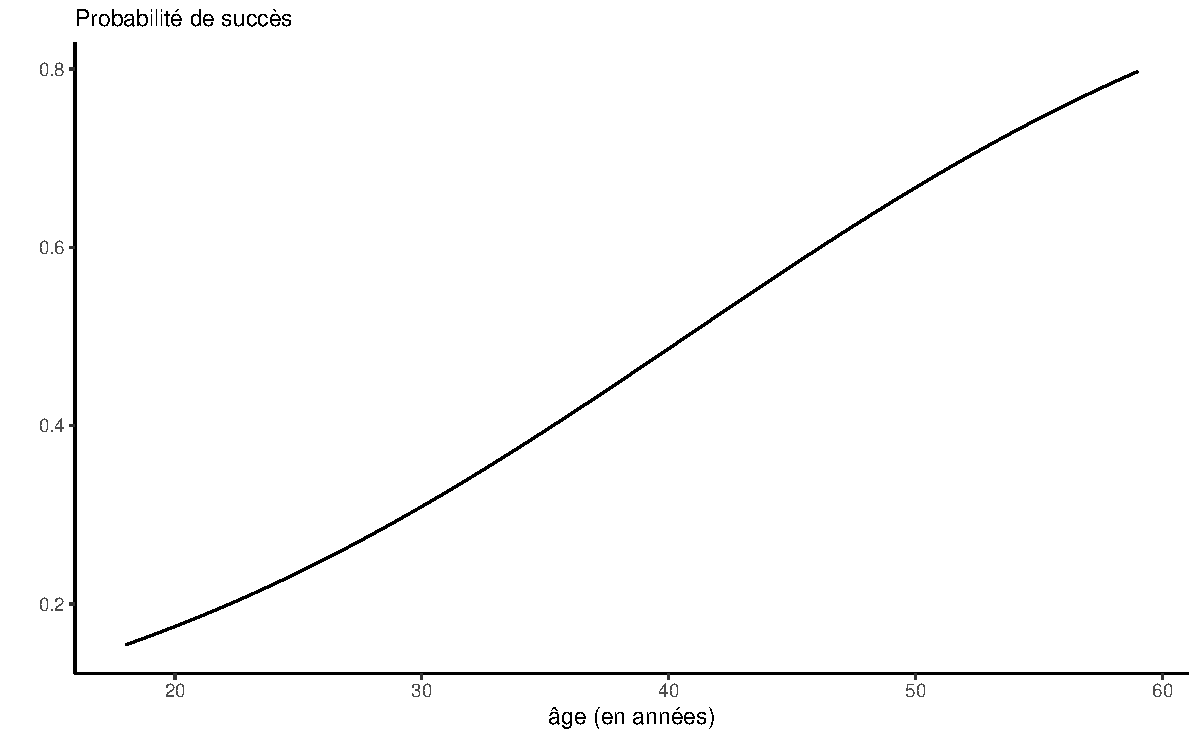
\includegraphics[width=0.8\textwidth,height=\textheight]{reglogistique_files/figure-pdf/fig-logitplot2-1.pdf}

}

\caption{\label{fig-logitplot2}Probabilité de suivre les recommendations
selon l'âge.}

\end{figure}%

\begin{itemize}
\tightlist
\item
  La valeur-\(p\) pour \(\widehat{\beta}_{\texttt{age}}\) correspondant
  au test des hypothèses \(\mathscr{H}_0: \beta_{\texttt{age}}=0\)
  versus \(\mathscr{H}_1: \beta_{\texttt{age}} \neq 0\), est plus petite
  que \(10^{-4}\) et donc l'effet de la variable âge est statistiquement
  différent de zéro. Plus l'âge augmente, plus la probabilité d'être
  intéressé à acheter un produit recommandé par le PRCA augmente.
\end{itemize}

\subsection{Interprétation du
paramètre}\label{interpruxe9tation-du-paramuxe8tre}

Si une variable est modélisée à l'aide d'un seul paramètre (pas de terme
quadratique et pas d'interaction avec d'autre covariables), une valeur
positive du paramètre indique une association positive avec \(p\) alors
qu'une valeur négative indique le contraire.

Ainsi, le signe du paramètre donne le sens de l'association. Si le
coefficient \(\beta_j\) de la variable \(\mathrm{X}_j\) est positif,
alors plus la variable augmente, plus \(\Pr(Y=1)\) augmente.
Inversement, si le coefficient \(\beta_j\) est négatif, plus la variable
augmente, plus \(\Pr(Y=1)\) diminue.

En régression linéaire, l'interprétation de coefficient \(\beta_j\) est
simple: lorsque la variable \(\mathrm{X}_j\) augmente de un, la variable
\(Y\) augmente en moyenne de \(\beta_j\), toute chose étant égale par
ailleurs. Cette interprétation ne dépend pas de la valeur de
\(\mathrm{X}_j\). En régression logistique, comme le modèle est
nonlinéaire en fonction de \(\Pr(Y=1)\) (courbe sigmoide),
l'augmentation ou la dimininution de \(\Pr(Y=1\mid \mathbf{X})\) pour un
changement d'une unité de \(\mathrm{X}_j\) dépend de la valeur de cette
dernière. C'est pourquoi il est parfois plus utile d'utiliser la cote
pour interpréter globalement l'effet d'une variable.

Dans notre exemple, on peut exprimer le modèle ajusté en termes de cote,
\begin{align*}
 \frac{\Pr(Y=1 \mid \mathrm{X}_5=x_5)}{\Pr(Y=0 \mid \mathrm{X}_5=x_5)} = \exp(-3.05)\exp(0.0749x_5).
\end{align*} Ainsi, lorsque \(\mathrm{X}_5\) augmente d'une année, la
cote est multipliée par \(\exp(0.0749) = 1.078\) peut importe la valeur
de \(x_5\). Pour deux personnes dont la différence d'âge est un an, la
cote de la personne plus âgée est 7.8\% plus élevée. On peut aussi
quantifier l'effet d'une augmentation d'un nombre d'unités quelconque.
Par exemple, pour chaque augmentation de 10 ans de \(\mathrm{X}_5\), la
cote est multiplié par \(1.078^{10} = 2.12\), soit une augmentation de
112\%.

L'interprétation des coefficients du modèle logistique se fait au niveau
du rapport de cote, à savoir \(\exp(\beta)\).

Un des avantages d'utiliser la vraisemblance comme fonction objective
est que les intervalles de confiance et les estimateurs basés sur la
vraisemblance (profilée) sont invariant aux reparamétrisations:
l'intervalle de confiance à niveau 95\% pour
\(\exp(\beta_{\texttt{age}})\) est obtenu en prenant l'exponentielle des
bornes de l'intervalle pour \(\beta_{\texttt{age}}\),
{[}\(\exp(0.0465); \exp(0.1043)\){]}, soit {[}\(1.048; 1.110\){]} tel
que rapporté dans la sortie. Ce n'est \textbf{pas} le cas des
intervalles usuels de Wald qui ont la forme
\(\widehat{\beta} \pm 1.96 \mathrm{se}(\widehat{\beta})\).

Comme l'exponentielle est une transformation monotone croissante, on a
\(\beta>0\) si et seulement si \(\exp(\beta)>1\), etc. On peut ainsi
utiliser les intervalles de confiance pour tester l'hypothèse
\(\mathscr{H}_0: \beta_j=0\) ou de façon équivalente
\(\mathscr{H}_0: \exp(\beta_j)=1\) à niveau 95\%.

Ajustons à présent le modèle avec toutes les variables explicatives.
Rappelez-vous que la variable \(\mathrm{X}_1\) (quel genre d'emploi
occupez-vous) a cinq catégories, \(\mathrm{X}_2\) (revenu familial
annuel) a cinq catégories, et \(\mathrm{X}_6\) (combien de fois
avez-vous assisté à un rodéo au cours de la dernière année) a trois
catégories. Notez qu'on pourrait aussi traiter \(\mathrm{X}_2\) comme
continue car elle est ordinale et possède tout de même cinq modalités,
mais on la traitera comme variable nominale.

Les variables de type \texttt{factor} sont modélisées par défaut à
l'aide d'un ensemble de variables indicatrices, la catégorie de
référence étant celle qui apparaît en dernier en ordre alphabétique.

\begin{Shaded}
\begin{Highlighting}[]
\FunctionTok{str}\NormalTok{(logit1)}
\NormalTok{modele2 }\OtherTok{\textless{}{-}} \FunctionTok{glm}\NormalTok{(}
\NormalTok{  y }\SpecialCharTok{\textasciitilde{}}\NormalTok{ x1 }\SpecialCharTok{+}\NormalTok{ x2 }\SpecialCharTok{+}\NormalTok{ x3 }\SpecialCharTok{+}\NormalTok{ x4 }\SpecialCharTok{+}\NormalTok{ x5 }\SpecialCharTok{+}\NormalTok{ x6,}
  \AttributeTok{data =}\NormalTok{ logit1,}
  \AttributeTok{family =} \FunctionTok{binomial}\NormalTok{(}\AttributeTok{link =} \StringTok{"logit"}\NormalTok{)}
\NormalTok{)}
\FunctionTok{summary}\NormalTok{(modele2)}
\NormalTok{ic }\OtherTok{\textless{}{-}} \FunctionTok{confint}\NormalTok{(modele2)}
\CommentTok{\# Tests de rapport de vraisemblance}
\NormalTok{car}\SpecialCharTok{::}\FunctionTok{Anova}\NormalTok{(modele2, }\AttributeTok{type =} \StringTok{"3"}\NormalTok{)}
\end{Highlighting}
\end{Shaded}

\begingroup
\setlength\LTleft{0\linewidth}
\setlength\LTright{0\linewidth}\fontsize{12.0pt}{14.4pt}\selectfont
\setlength{\LTpost}{0mm}

\begin{longtable}{@{\extracolsep{\fill}}lccc}

\toprule
variables & cote\textsuperscript{\textit{1}} & \textbf{95\% CI}\textsuperscript{\textit{1}} & valeur-p \\ 
\midrule\addlinespace[2.5pt]
{\bfseries x1} &  &  & 0.4 \\ 
    1 & — & — &  \\ 
    2 & 0.44 & 0.18, 1.06 &  \\ 
    3 & 0.51 & 0.21, 1.21 &  \\ 
    4 & 0.51 & 0.21, 1.25 &  \\ 
    5 & 0.70 & 0.27, 1.80 &  \\ 
{\bfseries x2} &  &  & <0.001 \\ 
    1 & — & — &  \\ 
    2 & 0.83 & 0.38, 1.82 &  \\ 
    3 & 0.57 & 0.25, 1.31 &  \\ 
    4 & 0.09 & 0.03, 0.25 &  \\ 
    5 & 0.26 & 0.08, 0.84 &  \\ 
{\bfseries x3} &  &  & <0.001 \\ 
    0 & — & — &  \\ 
    1 & 3.85 & 2.34, 6.50 &  \\ 
{\bfseries x4} &  &  & <0.001 \\ 
    0 & — & — &  \\ 
    1 & 6.24 & 3.53, 11.4 &  \\ 
{\bfseries x5} & 1.12 & 1.08, 1.16 & <0.001 \\ 
{\bfseries x6} &  &  & <0.001 \\ 
    1 & — & — &  \\ 
    2 & 0.25 & 0.13, 0.49 &  \\ 
    3 & 0.09 & 0.04, 0.18 &  \\ 
\bottomrule

\caption{\label{tbl-logit1-complet}Coefficients (cote), intervalles de
confiance profilée de 95 pourcent et valeurs-p pour le test de rapport
de vraisemblance pour le modèle logistique avec toutes les variables
catégorielles.}

\tabularnewline

\end{longtable}

\begin{minipage}{\linewidth}
\textsuperscript{\textit{1}}cote = rapport de cote, IC = intervalle de confiance\\
\end{minipage}
\endgroup

\begin{figure}[ht!]

\centering{

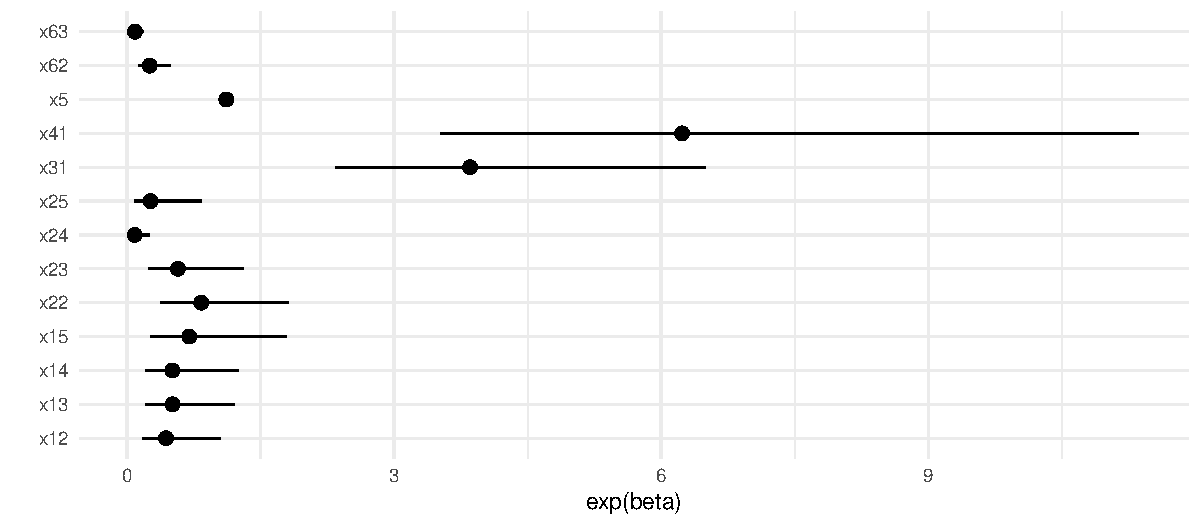
\includegraphics[width=1\textwidth,height=\textheight]{reglogistique_files/figure-pdf/fig-confint-modele2-logist-1.pdf}

}

\caption{\label{fig-confint-modele2-logist}Intervalles de confiance
profilés de niveau 95\% pour les coefficients du modèle logistique
(échelle exponentielle).}

\end{figure}%

\begin{longtable}[]{@{}lrrr@{}}

\caption{\label{tbl-gof-logist1}Mesures d'ajustement du modèle avec
toutes les variables explicatives, et du modèle nul (pour lequelle la
probabilité de succès est la proportion de 1).}

\tabularnewline

\toprule\noalign{}
& AIC & BIC & log.vrais. \\
\midrule\noalign{}
\endhead
\bottomrule\noalign{}
\endlastfoot
modèle ajusté & 544 & 603 & -258 \\
modèle nul & 691 & 695 & -258 \\

\end{longtable}

L'interprétation se fait comme en régression linéaire multiple puisqu'il
n'y a pas ni terme quadratique, ni interaction. Les paramètres estimés
représentent donc l'effet de la variable correspondante sur le logit une
fois que les autres variables sont dans le modèle, et demeurent fixes.

Prenons le coefficient associé à l'âge (\(\mathrm{X}_5\)) comme exemple.
Le paramètre estimé est \(\widehat{\beta}_{\texttt{age}}=0.109\) et il
est significativement différent de zéro. Ainsi, plus l'âge augmente,
plus \(\Pr(Y=1\mid \mathbf{X})\) augmente, toutes autres choses étant
égales par ailleurs. Pour chaque augmentation d'un an de
\(\mathrm{X}_5\), la cote est multipliée par \(\exp(0.109)=1.116\),
lorsque les autres variables demeurent fixes.

N'oubliez pas la nuance suivante concernant l'interprétation d'un test
lorsque plusieurs variables explicatives font partie du modèle. Si un
paramètre n'est pas significativement différent de zéro, cela ne veut
pas dire qu'il n'y a pas de lien entre la variable correspondante et
\(Y\). Cela veut seulement dire qu'il n'y a pas de lien significatif une
fois que les autres variables sont dans le modèle.

L'interprétation des variables catégorielles est analogue à celle faite
en régression linéaire. On peut aussi interpréter individuellement les
paramètres des indicatrices: pour \(\mathrm{I}(\mathrm{X}_6=2)\),
lorsque les autres variables demeurent fixes, les personnes ayant
assisté entre six et 10 fois à un rodéo au cours de la dernière année
voient leur cote multipliée par \(\exp(-1.370)=0.255\) par rapport aux
personnes ayant assisté plus de di fois. Ce paramètre est
significativement différent de zéro car sa valeur-\(p\) est négligeable;
l'intervalle de confiance à 95\% pour le rapport de cotes, basé sur la
vraisemblance profilée, est {[}0.13; 0.49{]} et la valeur 1 (qui
correspond à un rapport de cote constant) n'est pas dans l'intervalle.
Ainsi, il y a une différence significative entre les gens qui ont
assisté à 10 rodéos ou plus et les gens qui ont assisté à 5 rodéos ou
moins, pour ce qui est de l'intérêt à acheter un produit recommandé par
le PRCA.

Si on désire comparer les deux modalités \(\mathrm{X}_6=2\) et
\(\mathrm{X}_6=3\), il suffit de changer la modalité de référence de
\texttt{x6} et d'exécuter le modèle à nouveau. Une alternative est de
calculer le rapport de cotes pour ces deux modalités.

\subsection{Test du rapport de
vraisemblance}\label{test-du-rapport-de-vraisemblance}

Les tests rapportés d'ordinaire dans le tableau avec les coefficients
(et correspondants aux valeurs-\(p\)) sont des tests de Wald, à savoir
\(W = \widehat{\beta}/\widehat{\mathsf{se}}(\widehat{\beta})\). Ces
tests feront l'affaire dans la plupart des applications. Par contre, il
existe un autre test qui est généralement plus puissant, c'est-à-dire
qu'il sera meilleur pour détecter que \(\mathscr{H}_0\) n'est pas vraie
lorsque c'est effectivement le cas. Ce test est le test du rapport de
vraisemblance (\emph{likelihood ratio test}). Il découle de la méthode
d'estimation du maximum de vraisemblance et est donc généralement
applicable lorsqu'on estime les paramètres avec cette méthode. Il est
basé sur la quantité \(\ell\) que nous avons vue plus tôt.

La procédure consiste à ajuster deux modèles \textbf{emboîtés}:

\begin{itemize}
\tightlist
\item
  Le premier modèle, le modèle complet, contient tous les paramètres et
  l'estimateur du maximum de vraisemblance
  \(\widehat{\boldsymbol{\beta}})\).
\item
  Le deuxième modèle correspondant à l'hypothèse nulle
  \(\mathscr{H}_0\), le modèle réduit, contient tous les paramètres avec
  les restrictions imposées sous \(\mathscr{H}_0\); on dénote
  l'estimateur du maximum de vraisemblance
  \(\widehat{\boldsymbol{\beta}}_0\)
\end{itemize}

Le test est basé sur la statistique \begin{align*}
 D = -2\{\ell(\widehat{\boldsymbol{\beta}}_0)-\ell(\widehat{\boldsymbol{\beta}})\}.
\end{align*} Cette différence \(D\), lorsque l'hypothèse
\(\mathscr{H}_0\) est vraie suit approximativement une loi khi-deux avec
un nombre de degrés de liberté égal au nombre de paramètre testé (le
nombre de restrictions sous \(\mathscr{H}_0\)). On peut donc calculer la
valeur-\(p\) en utilisant la distribution du khi-deux.

Prenons comme exemple le test de la significativité de \(\mathrm{X}_6\),
qui est modélisée à l'aide deux variables binaires et dont les
paramètres correspondants sont \(\beta_{6_{\texttt{2}}}\) et
\(\beta_{6_{\texttt{3}}}\). Pour effectuer le test du rapport de
vraisemblance, il suffit de retirer la variable \(\mathrm{X}_6\) et de
réajuster le modèle à nouveau avec toutes les autres variables.

\begin{Shaded}
\begin{Highlighting}[]
\CommentTok{\# Ajuster modèle sous H0 (sans X6)}
\NormalTok{modeleH0 }\OtherTok{\textless{}{-}} \FunctionTok{update}\NormalTok{(modele2, }\AttributeTok{formula. =}  \StringTok{". \textasciitilde{} . {-} x6"}\NormalTok{)}
\FunctionTok{anova}\NormalTok{(modeleH0, modele2, }\AttributeTok{test =} \StringTok{"LRT"}\NormalTok{)}
\CommentTok{\# Le modèle \textquotesingle{}modeleH0\textquotesingle{} est équivalent à }
\CommentTok{\# glm(y \textasciitilde{} x1 + x2 + x3 + x4 + x5,}
\CommentTok{\#  data = logit1, }
\CommentTok{\#  family = binomial(link = "logit"))}

\DocumentationTok{\#\# Calculer statistique du test manuellement}
\DocumentationTok{\#\# Deviance = {-}2*log vraisemblance}
\NormalTok{rvrais }\OtherTok{\textless{}{-}}\NormalTok{ modeleH0}\SpecialCharTok{$}\NormalTok{deviance }\SpecialCharTok{{-}}\NormalTok{ modele2}\SpecialCharTok{$}\NormalTok{deviance}
\CommentTok{\# Valeur{-}p}
\FunctionTok{pchisq}\NormalTok{(rvrais, }\AttributeTok{df =} \DecValTok{2}\NormalTok{, }\AttributeTok{lower.tail =} \ConstantTok{FALSE}\NormalTok{)}
\end{Highlighting}
\end{Shaded}

Considérons maintenant la variable \(\mathrm{X}_6\), qui représente le
nombre de fois où l'individu a assisté à un rodéo au cours de la
dernière année. Cette variable est modélisée à l'aide de deux variables
indicatrices, \(\mathrm{I}(\mathrm{X}_6=2)\) égale à un si
\(\mathrm{X}_6=2\) et zéro autrement, et \(\mathrm{I}(\mathrm{X}_6=3)\)
égale à un si \(\mathrm{X}_6=3\) et zéro sinon. La catégorie de
référence est \(\mathrm{X}_6=1\), c'est-à-dire les personnes ayant
assisté plus de 10 fois à un rodéo au cours de la dernière année. Pour
tester la significativité globale d'une variable catégorielle qui est
modélisée avec plusieurs indicatrices, il faut utiliser un test qui
compare l'ajustement du modèle avec ou sans toutes les variables
binaires associées à \(\mathrm{X}_6\); l'hypothèse nulle
\(\mathscr{H}_0: \beta_{6_{\texttt{2}}}=\beta_{6_{\texttt{3}}}=0\)
versus l'alternative qu'au moins un de ces deux paramètres est différent
de zéro. La statistique du test de rapport de vraisemblance \(D\) de
50.251 et la valeur-\(p\) peut-être obtenue de la loi du khi-deux avec 2
degrés de liberté via le code suivant permet d'imprimer la valeur-\(p\),
qui est \(1.22 \times 10^{-11}\).

\subsection{Multicolinéarité}\label{multicolinuxe9arituxe9}

Rappelez-vous que le terme multicolinéarité fait référence à la
situation où les variables explicatives sont très corrélées entre elles
ou bien, plus généralement, à la situation où une (ou plusieurs)
variable(s) explicative(s) est (sont) très corrélée(s) à une combinaison
linéaire des autres variables explicatives.

L'effet potentiellement néfaste de la multicolinéarité est le même qu'en
régression linéaire, c'est-à-dire, elle peut réduire la précision des
estimations des paramètres (augmenter leurs écarts-types estimés).

En pratique, le problème est qu'il devient difficile de départager
l'effet individuel d'une variable explicative lorsqu'elle est fortement
corrélée avec d'autres variables explicatives.

Comme la multicolinéarité est une propriété des variables explicatives
(le \(Y\) n'intervient pas) on peut utiliser les mêmes outils qu'en
régression linéaire pour tenter de la détecter, par exemple, le facteur
d'inflation de la variance (\emph{variance inflation factor}),
accessible via \texttt{car::vif} pour un modèle de régression. Cette
quantité ne dépend que des variables explicatives \(\mathbf{X}\), pas du
modèle ou de la variable réponse.

La multicolinéarité est surtout un problème lorsque vient le temps
d'interpréter et tester l'effet des paramètres individuels. Si le but
est seulement de faire de la classification (prédiction) et que
l'interprétation des paramètres individuels n'est pas cruciale alors il
n'y a pas lieu de se soucier de la multicolinéarité. Il faut alors
plutôt comparer correctement la performance de classification des
modèles en utilisant des méthodes permettant d'obtenir un bon modèle
tout en se protégeant contre le surajustement. Certaines de ces méthodes
(division de l'échantillon, validation croisée) ont déjà été présentées.

\begin{tcolorbox}[enhanced jigsaw, bottomrule=.15mm, toptitle=1mm, opacityback=0, title=\textcolor{quarto-callout-note-color}{\faInfo}\hspace{0.5em}{En résumé}, left=2mm, bottomtitle=1mm, colbacktitle=quarto-callout-note-color!10!white, colback=white, breakable, toprule=.15mm, coltitle=black, arc=.35mm, opacitybacktitle=0.6, colframe=quarto-callout-note-color-frame, titlerule=0mm, leftrule=.75mm, rightrule=.15mm]

\begin{itemize}
\tightlist
\item
  Une régression logistique sert à modéliser la moyenne de
  \textbf{variables catégorielles}, typiquement binaires.
\item
  C'est un cas particulier d'un modèle de régression linéaire
  généralisée.
\item
  Le modèle est interprétable à l'échelle de la cote, qui donne dans le
  cas binaire le rapport probabilité de réussite (1) sur probabilité
  d'échec (0)
\item
  En l'absence d'interactions, on interprète les coefficients en terme
  de pourcentage d'augmentation si \(\exp(\widehat{\beta}) > 1\), avec
  \(\exp(\widehat{\beta})-1\) ou en terme de pourcentage de diminution
  si \(\exp(\widehat{\beta}) < 1\), avec \(1-\exp(\widehat{\beta})\)
\item
  L'estimation est faite par maximum de vraisemblance: on a accès aux
  critères d'information et aux tests d'hypothèses omnibus pour comparer
  des modèles emboîtés.
\item
  Les intervalles de confiance de vraisemblance profilée rapportés sont
  invariants aux reparamétrisations.
\end{itemize}

\end{tcolorbox}

\section{Classification et
prédiction}\label{classification-et-pruxe9diction}

La finalité du modèle de régression logistique est fréquemment
l'obtention de prédictions. Une fois qu'on a ajusté un modèle, on peut
l'utiliser pour prévoir la valeur de \(Y\) pour de nouvelles
observations. Ceci consiste à assigner une classe (\(0\) ou \(1\)) à ces
observations (pour lesquels \(Y\) est inconnue) à partir des valeurs
prises par \(\mathrm{X}_1, \ldots, \mathrm{X}_p\).

Le modèle ajusté nous fournit une estimation de
\(\Pr(Y=1 \mid \mathbf{X}=\boldsymbol{x})\) pour des valeurs
\(\mathrm{X}_1=x_1, \ldots, \mathrm{X}_p=x_p\) données. Cet estimé est
\begin{align*}
 \widehat{p} = \frac{1}{1+ \exp\{- ( \widehat{\beta}_0 + \widehat{\beta}_1x_1 + \cdots + \widehat{\beta}_p x_p)\}}.
\end{align*}

Classification de base: pour classifier des observations, il suffit de
choisir un point de coupure \(c\), souvent \(c=0.5\), et de classifier
une observation de la manière suivante:

\begin{itemize}
\tightlist
\item
  Si \(\widehat{p} < c\), on assigne cette observation à la catégorie
  zéro et \(\widehat{Y}=0\).
\item
  Si \(\widehat{p} \geq c\), on assigne cette observation à la catégorie
  un et \(\widehat{Y}=1\).
\end{itemize}

Si on prend \(c=0.5\) comme point de coupure, cela revient à assigner
l'observation à la classe (catégorie) la plus probable, un choix fort
raisonnable. Nous verrons dans une section suivante que, lorsque les
conséquences de faussement classifier une observation (succès, mais
échec prédit et vice-versa) ne sont pas les mêmes, il peut être
avantageux d'utiliser un autre point de coupure.

Dans un cadre de prédiction, il nous faudra un critère pour juger de la
qualité de l'ajustement du modèle. Rappelez-vous que pour une réponse
continue, nous avons utilisé l'erreur quadratique moyenne,
\(\mathsf{EQM} = \mathsf{E}\{(Y-\widehat{Y})^2\}\), où
\(\widehat{Y} = \mathsf{E}(Y \mid \mathbf{X})\), pour juger de la
performance d'un modèle. Comme la réponse \(Y\) est binaire ici, nous
allons utiliser des critères différents.

Voyons d'abord un premier critère pour juger de la qualité d'un modèle
de prédiction. Soit \(Y\) la vraie valeur de la réponse binaire et
\(\widehat{Y}\) (soit 0 ou 1) la valeur de \(Y\) prédite par un modèle
pour une observation choisie au hasard dans la population. Un premier
critère pour juger de la performance d'un modèle est le \textbf{taux de
mauvaise classification}, un estimé de la probabilité de mal classifier
une observation choisie au hasard dans la population,
\(\Pr(Y \neq\widehat{Y})\). Plus \(\Pr(Y \neq\widehat{Y})\) est petite,
meilleure est la capacité prédictive du modèle.

Tout comme l'erreur quadratique moyenne, on ne peut qu'estimer
\(\Pr(Y \neq\widehat{Y})\). Pour les raisons vues au chapitre précédent,
l'estimer en calculant le taux de mauvaise classification des
observations ayant servi à l'ajustement du modèle sans aucune correction
n'est pas une bonne approche. Les approches couvertes dans le dernier
chapitre pour l'estimation de l'erreur quadratique moyenne, telles la
validation-croisée et la division de l'échantillon, peuvent être
utilisées pour estimer le taux de mauvaise classification
\(\Pr(Y \neq \widehat{Y})\).

Cette utilisation d'un modèle de régression logistique sera illustrée
avec l'exemple que nous avons traité au chapitre précédent: notre
objectif final est de construire un modèle avec les 1000 clients de
l'échantillon d'apprentissage et cibler ensuite lesquels des 100 000
clients restants seront choisis pour recevoir le catalogue. Les
variables cibles sont:

\begin{itemize}
\tightlist
\item
  \texttt{yachat}: variable binaire égale à un si le client a acheté
  quelque chose dans le catalogue et zéro sinon.
\item
  \texttt{ymontant}: le montant de l'achat si le client a acheté quelque
  chose
\end{itemize}

Les 10 variables suivantes sont disponibles pour tous les clients et
serviront de variables explicatives,

\begin{itemize}
\tightlist
\item
  \texttt{x1}: sexe de l'individu, soit homme (0) ou femme (1);
\item
  \texttt{x2}: l'âge (en année);
\item
  \texttt{x3}: variable catégorielle indiquant le revenu, soit moins de
  35 000\$ (1), entre 35 000\$ et 75 000\$ (2) ou plus de 75 000\$ (3);
\item
  \texttt{x4}: variable catégorielle indiquant la région où habite le
  client (de 1 à 5);
\item
  \texttt{x5}: conjoint : le client a-t-il un conjoint, soit oui (1) ou
  non (0);
\item
  \texttt{x6}: nombre d'année depuis que le client est avec la
  compagnie;
\item
  \texttt{x7}: nombre de semaines depuis le dernier achat;
\item
  \texttt{x8}: montant (en dollars) du dernier achat;
\item
  \texttt{x9}: montant total (en dollars) dépensé depuis un an;
\item
  \texttt{x10}: nombre d'achats différents depuis un an.
\end{itemize}

Dans le chapitre précédent, nous avons cherché à développer un modèle
pour prévoir \texttt{ymontant}, le montant dépensé, étant donné que le
client achète quelque chose. Cette fois-ci, nous allons travailler avec
la variable \texttt{yachat}, qui est binaire, à l'aide de la régression
logistique.

Afin d'introduire différentes notions, nous allons, dans un premier
temps, utiliser les 10 variables de base. À partir de la section
suivante, nous chercherons à optimiser le modèle en considérant les
interactions d'ordre deux.

\begin{Shaded}
\begin{Highlighting}[]
\FunctionTok{data}\NormalTok{(dbm, }\AttributeTok{package =} \StringTok{"hecmulti"}\NormalTok{)}
\NormalTok{formule }\OtherTok{\textless{}{-}} \FunctionTok{formula}\NormalTok{(}\StringTok{"yachat \textasciitilde{} x1 + x2 + x3 +}
\StringTok{                x4 + x5 + x6 + x7 + x8 + x9 + x10"}\NormalTok{)}
\NormalTok{dbm\_class }\OtherTok{\textless{}{-}}\NormalTok{ dbm }\SpecialCharTok{|\textgreater{}}
\NormalTok{  dplyr}\SpecialCharTok{::}\FunctionTok{filter}\NormalTok{(test }\SpecialCharTok{==} \DecValTok{0}\NormalTok{) }\SpecialCharTok{|\textgreater{}}
\NormalTok{  dplyr}\SpecialCharTok{::}\FunctionTok{mutate}\NormalTok{(}\AttributeTok{yachat =} \FunctionTok{factor}\NormalTok{(yachat))}
\FunctionTok{set.seed}\NormalTok{(}\DecValTok{202209}\NormalTok{)}
\NormalTok{predprob }\OtherTok{\textless{}{-}}\NormalTok{ hecmulti}\SpecialCharTok{::}\FunctionTok{predvc}\NormalTok{(}
  \AttributeTok{modele =} \FunctionTok{glm}\NormalTok{(}\AttributeTok{formula =}\NormalTok{ formule, }
               \AttributeTok{data =}\NormalTok{ dbm\_class, }
               \AttributeTok{family =}\NormalTok{ binomial),}
  \AttributeTok{K =} \DecValTok{10}\NormalTok{, }\CommentTok{\#nombre de plis}
  \AttributeTok{nrep =} \DecValTok{1}\NormalTok{,}
  \AttributeTok{type =} \StringTok{"response"}\NormalTok{)}
\NormalTok{classif }\OtherTok{\textless{}{-}} \FunctionTok{with}\NormalTok{(dbm, yachat[test }\SpecialCharTok{==} \DecValTok{0}\NormalTok{])}
\CommentTok{\# Tableau de la performance}
\NormalTok{hecmulti}\SpecialCharTok{::}\FunctionTok{perfo\_logistique}\NormalTok{(}
  \AttributeTok{prob =}\NormalTok{ predprob,}
  \AttributeTok{resp =}\NormalTok{ classif)}
\end{Highlighting}
\end{Shaded}

Le modèle utilise seulement les 10 variables de base. Des prévisions
pour les clients restants seront exportées dans le fichier. La méthode
\texttt{predict} permet d'obtenir les prédictions des probabilités et la
fonction maison \texttt{hecmulti::perfo\_logistique} retourne un tableau
de classification. Tel que nous l'avons vu au chapitre précédent, il y a
210 clients qui ont acheté quelque chose parmi les 1000.

\begin{figure}[ht!]

\centering{

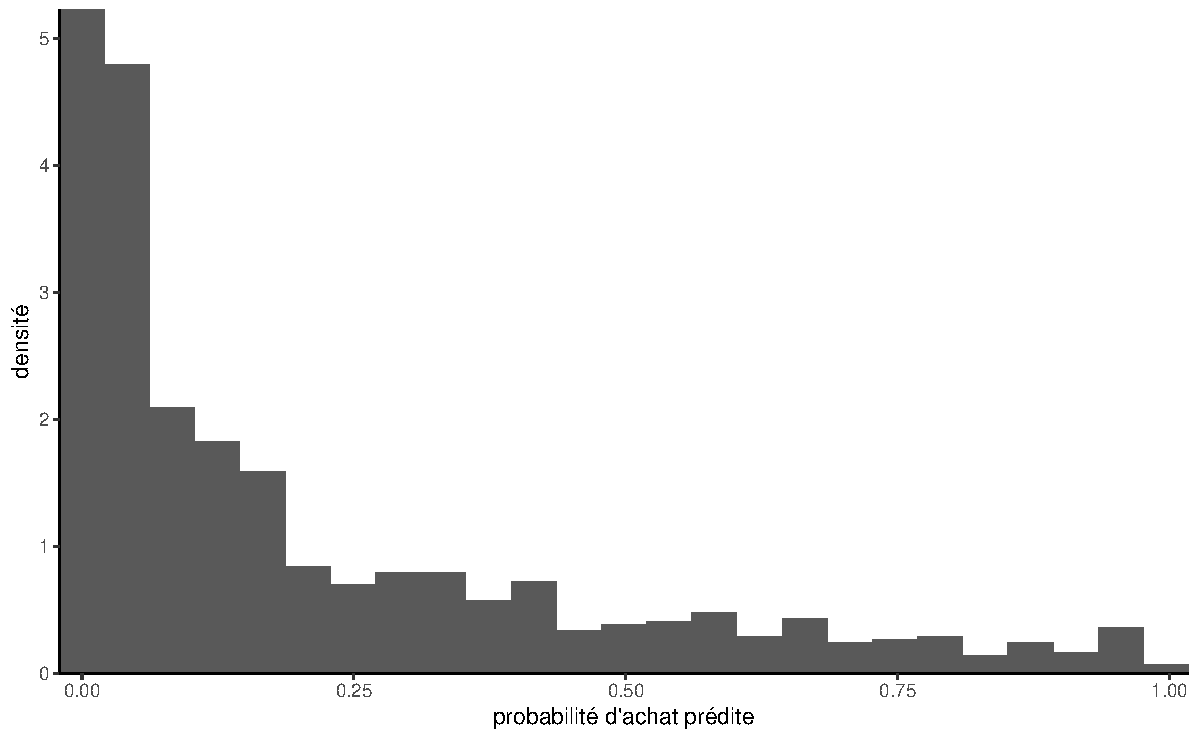
\includegraphics[width=0.85\textwidth,height=\textheight]{reglogistique_files/figure-pdf/fig-classification0-1.pdf}

}

\caption{\label{fig-classification0}Répartition des probabilités de
succès prédites par validation croisée à \(n\) groupes.}

\end{figure}%

\begin{longtable}[]{@{}
  >{\raggedleft\arraybackslash}p{(\columnwidth - 18\tabcolsep) * \real{0.0769}}
  >{\raggedleft\arraybackslash}p{(\columnwidth - 18\tabcolsep) * \real{0.0513}}
  >{\raggedleft\arraybackslash}p{(\columnwidth - 18\tabcolsep) * \real{0.0513}}
  >{\raggedleft\arraybackslash}p{(\columnwidth - 18\tabcolsep) * \real{0.0513}}
  >{\raggedleft\arraybackslash}p{(\columnwidth - 18\tabcolsep) * \real{0.0513}}
  >{\raggedleft\arraybackslash}p{(\columnwidth - 18\tabcolsep) * \real{0.1538}}
  >{\raggedleft\arraybackslash}p{(\columnwidth - 18\tabcolsep) * \real{0.2051}}
  >{\raggedleft\arraybackslash}p{(\columnwidth - 18\tabcolsep) * \real{0.2051}}
  >{\raggedleft\arraybackslash}p{(\columnwidth - 18\tabcolsep) * \real{0.0769}}
  >{\raggedleft\arraybackslash}p{(\columnwidth - 18\tabcolsep) * \real{0.0769}}@{}}

\caption{\label{tbl-classification-loocv}Tableau de classification avec
le nombre de vrais positifs (VP), vrais négatifs (VN), faux positifs
(FP) et faux négatifs (FN), le taux de bonne classification, la
sensibilité, la spécificité, le taux de vrais positifs (TVP) et le taux
de vrais négatifs (TVN).}

\tabularnewline

\toprule\noalign{}
\begin{minipage}[b]{\linewidth}\raggedleft
coupe
\end{minipage} & \begin{minipage}[b]{\linewidth}\raggedleft
VP
\end{minipage} & \begin{minipage}[b]{\linewidth}\raggedleft
VN
\end{minipage} & \begin{minipage}[b]{\linewidth}\raggedleft
FP
\end{minipage} & \begin{minipage}[b]{\linewidth}\raggedleft
FN
\end{minipage} & \begin{minipage}[b]{\linewidth}\raggedleft
correct (\%)
\end{minipage} & \begin{minipage}[b]{\linewidth}\raggedleft
sensibilité (\%)
\end{minipage} & \begin{minipage}[b]{\linewidth}\raggedleft
spécificité (\%)
\end{minipage} & \begin{minipage}[b]{\linewidth}\raggedleft
TVP
\end{minipage} & \begin{minipage}[b]{\linewidth}\raggedleft
TVN
\end{minipage} \\
\midrule\noalign{}
\endhead
\bottomrule\noalign{}
\endlastfoot
0.02 & 210 & 209 & 581 & 0 & 41.9 & 100.0 & 26.5 & 26.5 & 100.0 \\
0.04 & 207 & 320 & 470 & 3 & 52.7 & 98.6 & 40.5 & 30.6 & 99.1 \\
0.06 & 201 & 398 & 392 & 9 & 59.9 & 95.7 & 50.4 & 33.9 & 97.8 \\
0.08 & 199 & 451 & 339 & 11 & 65.0 & 94.8 & 57.1 & 37.0 & 97.6 \\
0.10 & 193 & 480 & 310 & 17 & 67.3 & 91.9 & 60.8 & 38.4 & 96.6 \\
0.12 & 191 & 512 & 278 & 19 & 70.3 & 91.0 & 64.8 & 40.7 & 96.4 \\
0.14 & 184 & 547 & 243 & 26 & 73.1 & 87.6 & 69.2 & 43.1 & 95.5 \\
0.16 & 176 & 572 & 218 & 34 & 74.8 & 83.8 & 72.4 & 44.7 & 94.4 \\
0.18 & 172 & 598 & 192 & 38 & 77.0 & 81.9 & 75.7 & 47.3 & 94.0 \\
0.20 & 164 & 611 & 179 & 46 & 77.5 & 78.1 & 77.3 & 47.8 & 93.0 \\
0.22 & 162 & 626 & 164 & 48 & 78.8 & 77.1 & 79.2 & 49.7 & 92.9 \\
0.24 & 158 & 639 & 151 & 52 & 79.7 & 75.2 & 80.9 & 51.1 & 92.5 \\
0.26 & 153 & 645 & 145 & 57 & 79.8 & 72.9 & 81.6 & 51.3 & 91.9 \\
0.28 & 150 & 657 & 133 & 60 & 80.7 & 71.4 & 83.2 & 53.0 & 91.6 \\
0.30 & 143 & 667 & 123 & 67 & 81.0 & 68.1 & 84.4 & 53.8 & 90.9 \\
0.32 & 138 & 679 & 111 & 72 & 81.7 & 65.7 & 85.9 & 55.4 & 90.4 \\
0.34 & 134 & 695 & 95 & 76 & 82.9 & 63.8 & 88.0 & 58.5 & 90.1 \\
0.36 & 130 & 699 & 91 & 80 & 82.9 & 61.9 & 88.5 & 58.8 & 89.7 \\
0.38 & 126 & 708 & 82 & 84 & 83.4 & 60.0 & 89.6 & 60.6 & 89.4 \\
0.40 & 120 & 715 & 75 & 90 & 83.5 & 57.1 & 90.5 & 61.5 & 88.8 \\
0.42 & 115 & 723 & 67 & 95 & 83.8 & 54.8 & 91.5 & 63.2 & 88.4 \\
0.44 & 112 & 731 & 59 & 98 & 84.3 & 53.3 & 92.5 & 65.5 & 88.2 \\
0.46 & 109 & 736 & 54 & 101 & 84.5 & 51.9 & 93.2 & 66.9 & 87.9 \\
0.48 & 106 & 739 & 51 & 104 & 84.5 & 50.5 & 93.5 & 67.5 & 87.7 \\
0.50 & 100 & 744 & 46 & 110 & 84.4 & 47.6 & 94.2 & 68.5 & 87.1 \\
0.52 & 98 & 748 & 42 & 112 & 84.6 & 46.7 & 94.7 & 70.0 & 87.0 \\
0.54 & 92 & 750 & 40 & 118 & 84.2 & 43.8 & 94.9 & 69.7 & 86.4 \\
0.56 & 87 & 753 & 37 & 123 & 84.0 & 41.4 & 95.3 & 70.2 & 86.0 \\
0.58 & 83 & 761 & 29 & 127 & 84.4 & 39.5 & 96.3 & 74.1 & 85.7 \\
0.60 & 80 & 766 & 24 & 130 & 84.6 & 38.1 & 97.0 & 76.9 & 85.5 \\
0.62 & 77 & 769 & 21 & 133 & 84.6 & 36.7 & 97.3 & 78.6 & 85.3 \\
0.64 & 74 & 771 & 19 & 136 & 84.5 & 35.2 & 97.6 & 79.6 & 85.0 \\
0.66 & 68 & 772 & 18 & 142 & 84.0 & 32.4 & 97.7 & 79.1 & 84.5 \\
0.68 & 62 & 774 & 16 & 148 & 83.6 & 29.5 & 98.0 & 79.5 & 83.9 \\
0.70 & 54 & 775 & 15 & 156 & 82.9 & 25.7 & 98.1 & 78.3 & 83.2 \\
0.72 & 51 & 777 & 13 & 159 & 82.8 & 24.3 & 98.4 & 79.7 & 83.0 \\
0.74 & 49 & 778 & 12 & 161 & 82.7 & 23.3 & 98.5 & 80.3 & 82.9 \\
0.76 & 46 & 778 & 12 & 164 & 82.4 & 21.9 & 98.5 & 79.3 & 82.6 \\
0.78 & 41 & 781 & 9 & 169 & 82.2 & 19.5 & 98.9 & 82.0 & 82.2 \\
0.80 & 35 & 783 & 7 & 175 & 81.8 & 16.7 & 99.1 & 83.3 & 81.7 \\
0.82 & 33 & 783 & 7 & 177 & 81.6 & 15.7 & 99.1 & 82.5 & 81.6 \\
0.84 & 32 & 783 & 7 & 178 & 81.5 & 15.2 & 99.1 & 82.1 & 81.5 \\
0.86 & 28 & 784 & 6 & 182 & 81.2 & 13.3 & 99.2 & 82.4 & 81.2 \\
0.88 & 25 & 786 & 4 & 185 & 81.1 & 11.9 & 99.5 & 86.2 & 80.9 \\
0.90 & 21 & 787 & 3 & 189 & 80.8 & 10.0 & 99.6 & 87.5 & 80.6 \\
0.92 & 18 & 787 & 3 & 192 & 80.5 & 8.6 & 99.6 & 85.7 & 80.4 \\
0.94 & 14 & 788 & 2 & 196 & 80.2 & 6.7 & 99.7 & 87.5 & 80.1 \\
0.96 & 6 & 788 & 2 & 204 & 79.4 & 2.9 & 99.7 & 75.0 & 79.4 \\
0.98 & 2 & 790 & 0 & 208 & 79.2 & 1.0 & 100.0 & 100.0 & 79.2 \\

\end{longtable}

Le Tableau~\ref{tbl-classification-loocv} contient des estimations de
plusieurs quantités intéressantes rattachées à la classification, en
faisant varier le point de coupure. Pour chaque point de coupure, ces
estimations ont été obtenues par validation croisée à \(n\) groupes (en
anglais, \emph{leave-one-out cross-validation}, ou LOOCV). Ainsi, ces
estimations sont meilleures que les estimés sans ajustement aucun car
elles ne sont pas obtenues en utilisant les mêmes observations que
celles qui ont servi à estimer le modèle.

La colonne \texttt{Correct} donne le taux de bonne classification,
\(\Pr(Y = \widehat{Y})\): avec un point de coupure de \(0\), on
classifie toutes les observations à la classe achat (\(1\)), car
\(\widehat{p}\) est forcément plus grande que zéro. Le taux de bonne
classification dans ce cas de figure sera de \(21\)\%, puisque 210
individus ont acheté un produit dans le catalogue dans l'échantillon
d'apprentissage. L'autre extrême, avec un point de coupure \(c=1\),
donne un taux de bonne classification de \(79\)\%.

On peut chercher dans le tableau les points de coupure qui donnent le
meilleur taux de bonne classification. Ce dernier, à savoir 84.6\%, est
atteint par trois points de coupure, soit 0.52, soit 0.6, soit 0.62. Une
recherche plus fine donne 0.465 comme point de coupure optimal, avec un
taux de mauvaise classification de 15.3\%.

Avec une variable réponse binaire, il y a deux classifications possibles
et le tableau de confusion contient, en partant du coin supérieur gauche
et dans le sens des aiguilles d'une montre, le nombre de vrai positif
(\(Y=1\), \(\widehat{Y}=1\)), de faux positif (\(Y=0\),
\(\widehat{Y}=1\)), de vrai négatif (\(Y=0\), \(\widehat{Y}=0\)) et
finalement de faux négatif (\(Y=1\), \(\widehat{Y}=0\)). La
\textbf{matrice de confusion}, qui compare les vraies valeurs avec les
prédictions, peut être construite à partir des colonnes \texttt{VP},
\texttt{VN}, \texttt{FP} et \texttt{FN}. Ces nombres proviennent de la
validation croisée à \(n\) groupes et ne sont pas ceux qu'on obtiendrait
si on appliquait directement le modèle ajusté à notre échantillon. Le
taux de mauvaise classification est \((\mathsf{FP}+\mathsf{FN})/n\); une
estimation plus fiable serait obtenue en utilisant la validation croisée
à 10 groupes.

\begin{longtable}[]{@{}lrr@{}}

\caption{\label{tbl-confumat}Matrice de confusion avec point de coupure
0.465.}

\tabularnewline

\toprule\noalign{}
& \(Y=1\) & \(Y=0\) \\
\midrule\noalign{}
\endhead
\bottomrule\noalign{}
\endlastfoot
\(\widehat{Y}=1\) & 109 & 52 \\
\(\widehat{Y}=0\) & 101 & 738 \\

\end{longtable}

Quatre autres quantités, dérivées à partir de la matrice de confusion,
sont parfois utilisées:

\begin{itemize}
\tightlist
\item
  la \textbf{sensibilité} (\emph{sensitivity}),
  \(\Pr(\widehat{Y}=1 \mid Y=1)\), ou
  \(\mathsf{VP}/(\mathsf{VP}+\mathsf{FN})\);
\item
  la \textbf{spécificité} (\emph{specificity}),
  \(\Pr(\widehat{Y}=0 \mid Y=0)\), ou
  \(\mathsf{VN}/(\mathsf{VN}+\mathsf{FP})\);
\item
  le \textbf{taux de vrais positifs}, \(\Pr(Y=1 \mid \widehat{Y}=1)\),
  ou \(\mathsf{VP}/(\mathsf{VP}+\mathsf{FP})\);
\item
  le \textbf{taux de vrais négatifs}, \(\Pr(Y=0 \mid \widehat{Y}=0)\),
  ou \(\mathsf{VN}/(\mathsf{VN}+\mathsf{FN})\).
\end{itemize}

Les estimés empiriques sont simplement obtenus en calculant les rapports
du nombre d'observations dans chaque classe.

La sensibilité mesure à quel point notre modèle est performant pour
détecter un vrai positif (classe 1). La spécificité mesure à quel point
notre modèle est performant pour détecter un résultat négatif (classe
0). Plus le point de coupure augmente, plus la sensibilité et le taux de
faux positifs diminuent mais plus la spécificité et le taux de faux
négatifs augmentent.

\subsection{Fonction d'efficacité du
récepteur}\label{fonction-defficacituxe9-du-ruxe9cepteur}

La \textbf{fonction d'efficacité du récepteur}, parfois appelée courbe
ROC (\emph{receiver operating characteristic}) est parfois utilisée pour
représenter globalement la performance du modèle. Il s'agit du graphe de
la sensibilité en fonction de un moins la spécificité, en faisant varier
le point de coupure. Un modèle parfait aurait une sensibilité et une
spécificité égales à 1 (correspondant au coin supérieur gauche de la
fonction d'efficacité du récepteur). Ainsi, plus le couple
(\(1-\)spécificité, sensibilité) est près de (\(0\), \(1\)), meilleur
est le modèle. Par conséquent, plus la courbe ROC tend vers (\(0\),
\(1\)) meilleur est le pouvoir prévisionnel des variables.
L'\textbf{aire sous la courbe} (\emph{area under the curve}, ou AUC) est
souvent utilisée en parallèle comme mesure de la qualité: comme son nom
l'indique, c'est l'aire sous la courbe de la fonction d'efficacité du
récepteur.

La fonction \texttt{courbe\_roc} permet de tracer la courbe et de
calculer l'aire sous la courbe. Plus cette valeur est près de 1, mieux
c'est: une probabilité de 0.5 correspond à une allocation aléatoire,
représentée sur la fonction d'efficacité du récepteur par la ligne
diagonale.

\begin{figure}[ht!]

\centering{

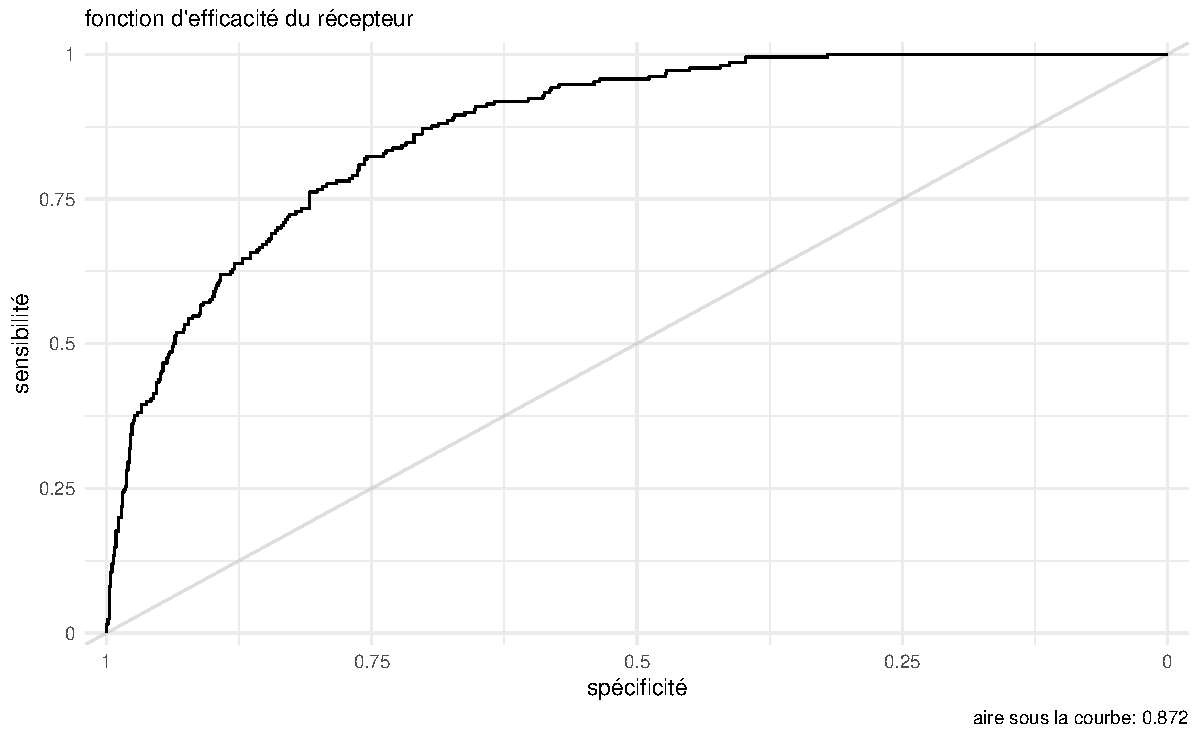
\includegraphics[width=0.8\textwidth,height=\textheight]{reglogistique_files/figure-pdf/fig-roccurve-1.pdf}

}

\caption{\label{fig-roccurve}Fonction d'efficacité du récepteur avec
probabilités de succès issues de la validation croisée à \(n\) groupes.}

\end{figure}%

\begin{Shaded}
\begin{Highlighting}[]
\CommentTok{\# Fonction d\textquotesingle{}efficacité du récepteur}
\NormalTok{roc }\OtherTok{\textless{}{-}}\NormalTok{ hecmulti}\SpecialCharTok{::}\FunctionTok{courbe\_roc}\NormalTok{(}
  \AttributeTok{resp =}\NormalTok{ classif,}
  \AttributeTok{prob =}\NormalTok{ predprob,}
  \AttributeTok{plot =} \ConstantTok{TRUE}\NormalTok{)}
\FunctionTok{print}\NormalTok{(roc)}
\DocumentationTok{\#\# Pour extraire l\textquotesingle{}aire sous la courbe, }
\CommentTok{\# roc$aire}
\end{Highlighting}
\end{Shaded}

\subsection{Classification avec une matrice de
gain}\label{classification-avec-une-matrice-de-gain}

Utiliser le taux de mauvaise classification \(\Pr(Y \neq \widehat{Y})\),
comme critère de performance, revient au même que d'utiliser le taux de
bonne classification \(\Pr(Y=\widehat{Y})\), car
\(\Pr(Y \neq \widehat{Y}) = 1-\Pr(Y=\widehat{Y})\). On veut un modèle
avec un haut taux de bonne classification (ou un faible taux de mauvaise
classification).

Lorsqu'on utilise \(\Pr(Y \neq \widehat{Y})\) comme critère pour juger
de la qualité d'un modèle prévisionnel, on fait l'hypothèse que le gain
associé à bien classifier une observation dans la catégorie 0
lorsqu'elle est réellement dans la catégorie 0 est le même que celui
associé à classifier une observation dans la catégorie 1 lorsqu'elle est
réellement dans la catégorie 1: cela correspond à la matrice de gain.

\begin{longtable}[]{@{}llrr@{}}
\caption{Matrice de gain correspondant au taux de bonne
classification}\label{tbl-03-gain1}\tabularnewline
\toprule\noalign{}
& & observation & \\
\midrule\noalign{}
\endfirsthead
\toprule\noalign{}
& & observation & \\
\midrule\noalign{}
\endhead
\bottomrule\noalign{}
\endlastfoot
& gain & \(Y=1\) & \(Y=0\) \\
prédiction & \(\widehat{Y}=1\) & \(1\) & \(0\) \\
& \(\widehat{Y}=0\) & \(0\) & \(1\) \\
\end{longtable}

Le gain vaut 1 lorsque la prévision est bonne (les deux cas sur la
diagonale) et 0 lorsque le modèle se trompe (les deux autres cas).
L'unité de mesure du gain n'est pas importante pour l'instant. Le gain
total est

\begin{align*}
\text{gain} &= 1 \Pr(\widehat{Y}=1, Y=1) + 1 \Pr(\widehat{Y}=0, Y=0)
\\ &\quad + 0 \Pr(\widehat{Y}=1, Y=0)  + 0 \Pr(\widehat{Y}=0, Y=1)
\\& = \Pr(Y = \widehat{Y}).
\end{align*} Maximiser le gain total revient donc à maximiser le taux de
bonne classification.

Dans certaines situations, les gains (ou la perte si le gain est
négatif) associés aux bonnes décisions et aux erreurs ne sont pas
équivalents.

Supposons que le gain de classer une observation à \(i\)
(\(i \in \{0,1\}\)) lorsqu'elle vaut \(j\) (\(j \in \{0,1\}\)) en
réalité est de \(c_{ij}\). La matrice de gain est alors

\begin{longtable}[]{@{}llrr@{}}
\caption{Matrice de gain pondérée en fonction d'un
coût}\label{tbl-03-gain2}\tabularnewline
\toprule\noalign{}
& & observation & \\
\midrule\noalign{}
\endfirsthead
\toprule\noalign{}
& & observation & \\
\midrule\noalign{}
\endhead
\bottomrule\noalign{}
\endlastfoot
& gain & \(Y=1\) & \(Y=0\) \\
prédiction & \(\widehat{Y}=1\) & \(c_{11}\) & \(c_{10}\) \\
& \(\widehat{Y}=0\) & \(c_{01}\) & \(c_{00}\) \\
\end{longtable}

En pratique, l'une de ces quatre quantités peut être fixée à 1 car
seulement les poids relatifs (les ratios) des gains sont importants.
Dans ce cas, le gain moyen est \begin{align*}
\text{gain} &= c_{11} \Pr(\widehat{Y}=1, Y=1) + c_{00}\Pr(\widehat{Y}=0, Y=0) 
\\ &\quad + c_{10} \Pr(\widehat{Y}=1, Y=0)  + c_{01} \Pr(\widehat{Y}=0, Y=1)
\end{align*}

Le meilleur modèle est alors celui qui maximise le gain moyen.

Nous allons encore une fois seulement utiliser les 10 variables de base.
Mais nous allons intégrer des revenus et coûts afin de trouver le
meilleur point de coupure. Rappelez-vous que le coût de l'envoi d'un
catalogue est de 10\$. Le tableau des variables descriptives qui suit
montre que, pour les 210 clients qui ont acheté quelque chose, le revenu
moyen est de 67.29\$ (moyenne de la variable \texttt{ymontant}).

\begin{longtable}[]{@{}rrrrr@{}}

\caption{\label{tbl-dbm-ymontant-apprentissage}Statistiques descriptives
des montants d'achats pour la base de données marketing (échantillon
d'apprentissage).}

\tabularnewline

\toprule\noalign{}
n & moyenne & écart-type & minimum & maximum \\
\midrule\noalign{}
\endhead
\bottomrule\noalign{}
\endlastfoot
210 & 67.3 & 13.2 & 25 & 109 \\

\end{longtable}

Nous allons travailler en termes de revenu net. Nous pouvons donc
spécifier la matrice de gain du Tableau~\ref{tbl-03-gain3} pour notre
problème. Si on n'envoie pas de catalogue, notre gain est nul. Si on
envoie le catalogue à un client qui n'achète pas, on perd 10\$ (le coût
de l'envoi). En revanche, notre revenu net est de 57\$ (revenu moyen
moins coût de l'envoi).

\begin{longtable}[]{@{}llrr@{}}
\caption{Matrice de gain pour l'envoi de
catalogue}\label{tbl-03-gain3}\tabularnewline
\toprule\noalign{}
& & observation & \\
\midrule\noalign{}
\endfirsthead
\toprule\noalign{}
& & observation & \\
\midrule\noalign{}
\endhead
\bottomrule\noalign{}
\endlastfoot
& gain & \(Y=1\) & \(Y=0\) \\
prédiction & \(\widehat{Y}=1\) & 57 & -10 \\
& \(\widehat{Y}=0\) & 0 & 0 \\
\end{longtable}

On peut calculer la performance du modèle et le gain moyen en faisant
varier le point de coupure. Pour avoir une mesure fidèle, on utilise la
validation croisée à \(K=10\) groupes (la mesure affichée correspondant
à la moyenne de 10 réplications)

\begin{Shaded}
\begin{Highlighting}[]
\FunctionTok{data}\NormalTok{(dbm, }\AttributeTok{package =} \StringTok{"hecmulti"}\NormalTok{)}
\NormalTok{donnees }\OtherTok{\textless{}{-}}\NormalTok{ dbm }\SpecialCharTok{|\textgreater{}} 
\NormalTok{  dplyr}\SpecialCharTok{::}\FunctionTok{filter}\NormalTok{(test }\SpecialCharTok{==} \DecValTok{0}\NormalTok{)}
\NormalTok{formule }\OtherTok{=} \FunctionTok{formula}\NormalTok{(yachat }\SpecialCharTok{\textasciitilde{}}\NormalTok{ x1 }\SpecialCharTok{+}\NormalTok{ x2 }\SpecialCharTok{+}\NormalTok{ x3 }\SpecialCharTok{+}
\NormalTok{                    x4 }\SpecialCharTok{+}\NormalTok{ x5 }\SpecialCharTok{+}\NormalTok{ x6 }\SpecialCharTok{+}\NormalTok{ x7 }\SpecialCharTok{+} 
\NormalTok{                    x8 }\SpecialCharTok{+}\NormalTok{ x9 }\SpecialCharTok{+}\NormalTok{ x10)}
\NormalTok{modele }\OtherTok{\textless{}{-}} \FunctionTok{glm}\NormalTok{(formule, }
              \AttributeTok{family =}\NormalTok{ binomial, }
              \AttributeTok{data =}\NormalTok{ donnees)}
\NormalTok{coupe }\OtherTok{\textless{}{-}}\NormalTok{ hecmulti}\SpecialCharTok{::}\FunctionTok{select\_pcoupe}\NormalTok{(}
  \AttributeTok{modele =}\NormalTok{ modele, }
  \AttributeTok{c00 =} \DecValTok{0}\NormalTok{, }
  \AttributeTok{c01 =} \DecValTok{0}\NormalTok{, }
  \AttributeTok{c10 =} \SpecialCharTok{{-}}\DecValTok{10}\NormalTok{, }
  \AttributeTok{c11 =} \DecValTok{57}\NormalTok{,}
  \AttributeTok{plot =} \ConstantTok{TRUE}\NormalTok{)}
\NormalTok{coupe}
\CommentTok{\#\textgreater{} Point de coupure optimal: 0.12}
\end{Highlighting}
\end{Shaded}

\begin{figure}[ht!]

\centering{

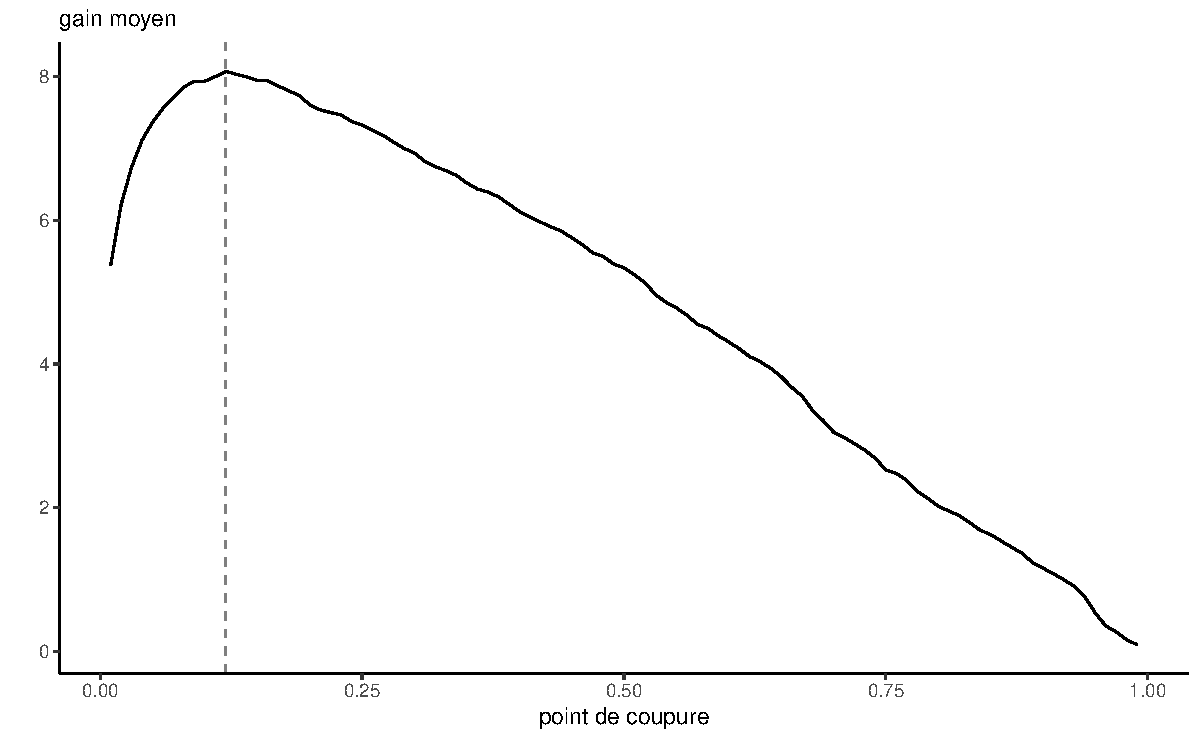
\includegraphics[width=0.85\textwidth,height=\textheight]{reglogistique_files/figure-pdf/fig-coupure-pondere-1.pdf}

}

\caption{\label{fig-coupure-pondere}Estimation du gain moyen en fonction
du point de coupure pour l'exemple de base de données marketing.}

\end{figure}%

La fonction \texttt{select\_pcoupe} donne l'estimation du gain moyen
(\texttt{gain}) pour différents points de coupures (\texttt{pcoupe}).
Cette estimation provient d'une validation-croisée avec \(K\) groupes
(\texttt{ncv}) dans la fonction), répétée \texttt{nrep} fois. On a
effectué ici la validation croisée avec 10 groupes et fait la moyenne
des 10 répétitions afin d'avoir plus de précision.

On voit dans la Figure~\ref{fig-coupure-pondere} que le meilleur point
de coupure, celui qui maximise le gain est 0.12. Avec ce point de
coupure, et selon le Tableau~\ref{tbl-classification-loocv}, on estime
que le taux de bonne classification est de 70.3 et que la sensibilité
est de 90.95. Ainsi, on estime qu'on va détecter environ 91\% des
clients qui achètent.

Comme il est très coûteux de rater un client qui aurait acheté quelque
chose, il est préférable d'envoyer le catalogue à plus de clients,
quitte à ce que plusieurs d'entre eux n'achètent rien. Bien que le point
de coupure de 0.5 donne un meilleur taux de bonne classification, il
correspond à un gain moyen plus faible car on rate trop de clients qui
achètent (la sensibilité est de seulement 47.62\%). Travailler avec la
matrice de gain permet de trouver le point de coupure optimal en
incorporant des notions de coûts et profits.

\subsection{Courbe lift}\label{courbe-lift}

Un autre type de graphe qui est souvent utilisé dans des contextes de
gestion est la courbe lift (sic) (en anglais, \emph{lift chart}). Cette
courbe est obtenue en ordonnant les probabilités de succès estimées par
le modèle, \(\widehat{p}\), en ordre croissant et en regardant quelle
pourcentage de ces derniers seraient bien classifiés (le nombre de vrais
positifs sur le nombre de succès). Elle sert dans le contexte où on a un
budget fixe, par exemple de publicité, et que l'on veut établir comment
une sélection (envoi ciblé) aurait performé par rapport à un envoi
systématique au même nombre de personnes.

\begin{Shaded}
\begin{Highlighting}[]
\NormalTok{tab\_lift }\OtherTok{\textless{}{-}}\NormalTok{ hecmulti}\SpecialCharTok{::}\FunctionTok{courbe\_lift}\NormalTok{(}
  \AttributeTok{prob =}\NormalTok{ predprob, }\CommentTok{\# probabilité de succès (Y=1)}
  \AttributeTok{resp =}\NormalTok{ classif, }\CommentTok{\# variable binaire réponse 0/1}
  \AttributeTok{plot =} \ConstantTok{TRUE}\NormalTok{)}
\NormalTok{tab\_lift}
\end{Highlighting}
\end{Shaded}

\begin{figure}[ht!]

\centering{

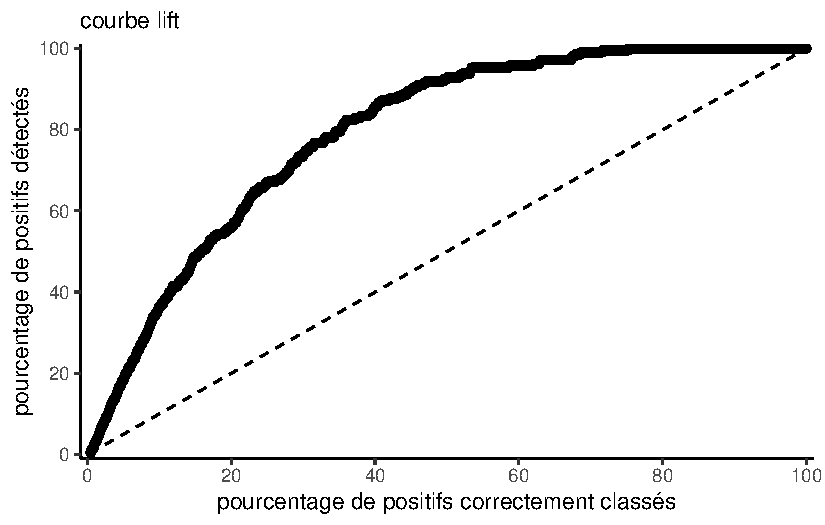
\includegraphics[width=0.85\textwidth,height=\textheight]{reglogistique_files/figure-pdf/fig-lift-1.pdf}

}

\caption{\label{fig-lift}Courbe lift}

\end{figure}%

\begin{longtable}[]{@{}lrrrr@{}}

\caption{\label{tbl-lift}Tableau du lift (déciles).}

\tabularnewline

\toprule\noalign{}
& pourcent & hasard & modele & lift \\
\midrule\noalign{}
\endhead
\bottomrule\noalign{}
\endlastfoot
10\% & 10 & 21 & 78 & 3.71 \\
20\% & 20 & 42 & 120 & 2.86 \\
30\% & 30 & 63 & 157 & 2.49 \\
40\% & 40 & 84 & 180 & 2.14 \\
50\% & 50 & 105 & 195 & 1.86 \\
60\% & 60 & 126 & 201 & 1.59 \\
70\% & 70 & 147 & 208 & 1.42 \\
80\% & 80 & 168 & 210 & 1.25 \\
90\% & 90 & 189 & 210 & 1.11 \\

\end{longtable}

Le Tableau~\ref{tbl-lift} présente les 10 déciles, mais on n'utilisera
en pratique qu'une seule valeur (correspondant à la fraction de clients
que l'on veut joindre). Si on classifiait comme acheteurs les 10\% qui
ont la plus forte probabilité estimée d'achat, on détecterait 81 des 210
clients (37.6\%). En comparaison, on s'attend que 21 clients soient
sélectionnés en moyenne si on prend un échantillon aléatoire de 100
personnes. Le ratio 81/21 (dernière colonne) est le \emph{lift} du
modèle: il permet de détecter 3.86 fois plus de succès que le hasard.

La Figure~\ref{fig-lift} présente le pourcentage d'observations bien
classées parmi les variables (pourcentage des probabilités prédites qui
correspondent à un succès parmi les \(k\) plus susceptibles selon le
modèle). La référence est la ligne diagonale, qui correspond à une
détection aléatoire.

\subsection{Calibration du modèle et détection du
surajustement}\label{calibration-du-moduxe8le-et-duxe9tection-du-surajustement}

Il peut être intéressant de vérifier la \textbf{calibration} de notre
modèle, et une statistique simple proposée par
\href{https://doi.org/10.1002/sim.4780050506}{Spiegelhalter (1986)} peut
être utile à cette fin. Pour une variable binaire \(Y \in \{0,1\}\),
l'erreur quadratique moyenne s'écrit \begin{align*}
\overline{B} &= \frac{1}{n} \sum_{i=1}^n (Y_i-p_i)^2 
=\frac{1}{n} \sum_{i=1}^n(Y_i-p_i)(1-2p_i) + \frac{1}{n} \sum_{i=1}^n p_i(1-p_i).
\end{align*} Le premier terme représente le manque de calibration du
modèle, tandis que le deuxième correspond à la séparation entre
variables. Si notre modèle était parfaitement calibré, alors
\(\mathsf{E}_0(Y_i)=p_i\) et \(\mathsf{Va}_0(Y_i) = p_i(1-p_i)\). On
peut utiliser ce fait pour construire une statistique de test de la
forme
\(Z = \{\overline{B} - \mathsf{E}_0(\overline{B})\}/\sqrt{\mathsf{Va}_0(\overline{B})}\),
où \begin{align*}
\mathsf{E}_0(\overline{B})&= \frac{1}{n} \sum_{i=1}^n p_i(1-p_i) \\
\mathsf{Va}_0(\overline{B})&= \frac{1}{n^2} \sum_{i=1}^n p_i(1-p_i)(1-2p_i)^2
\end{align*}

Sous l'hypothèse nulle de calibration parfaite,
\(Z \sim \mathsf{No}(0,1)\) en grand échantillon. Pour le modèle simple
avec toutes les covariables, la valeur-\(p\) approximative calculée avec
les probabilités de succès obtenues par validation-croisée et les
données de l'échantillon d'apprentissage est 0.22 et il n'y a pas de
preuve ici que le modèle est mal calibré. Cette technique est utile pour
vérifier s'il n'y a pas de surajustement (auquel cas le modèle tend à
retourner des probabilités très près de 0/1, mais qui ne correspondent
pas à la réalité).

Ici, nous avons ajusté un seul modèle, celui contenant uniquement les 10
variables de base et nous nous sommes attardés au choix du point de
coupure pour l'assignation aux classes. Il est possible qu'un autre
modèle, contenant par exemple des termes d'interactions, des termes
quadratiques ou d'autres transformations des variables, soit supérieur à
celui-ci. Le choix du modèle de prévision se fait donc souvent en deux
étapes:

\begin{enumerate}
\def\labelenumi{\arabic{enumi}.}
\tightlist
\item
  choisir les variables explicatives
\item
  sélectionner un point de coupure.
\end{enumerate}

Nous avons déjà vu des méthodes de sélections de variables au chapitre
précédent. La section suivante reviendra sur ces méthodes dans le
contexte de la régression logistique.

\subsection{Sélection de variables en régression
logistique}\label{suxe9lection-de-variables-en-ruxe9gression-logistique}

Les principes généraux, concernant la sélection de variables et de
modèles, que nous avons vus au chapitre précédent sont toujours valides.
Les critères \(\mathsf{AIC}\) et \(\mathsf{BIC}\) sont toujours
disponibles puisqu'on estime le modèle par maximum de vraisemblance et
les techniques générales de division de l'échantillon et de
validation-croisée sont toujours valides. La principale différence est
le coût d'estimation numérique des différents modèles: parce qu'il n'y a
pas de solution explicite pour les estimateurs du maximum de
vraisemblance du modèle logistique, ajuster chacun de ces modèles est
coûteux.

À la section précédente, nous avons inclus les 10 variables de base dans
notre exemple d'envoi ciblé. Nous allons ici faire une recherche de type
exhaustive parmi ces variables. La fonction \texttt{glmbb} du paquet
éponyme fait une recherche à l'aide de l'algorithme de recherche
arborescente dite par méthode de séparation et d'évaluation, qui ne
nécessite pas de tester tous les modèles emboîtés. La sortie inclut les
modèles qui sont à distance au plus \texttt{cutoff} du modèle optimal en
ordre décroissant du critère d'information, avec une pondération
associée qui peut servir comme succédané au mélange de modèle. La
fonction permet de choisir entre les critères \(\mathsf{AIC}\) et
\(\mathsf{BIC}\) et inclut toutes les modalités des variables
explicatives pour les facteurs.

\begin{Shaded}
\begin{Highlighting}[]
\FunctionTok{data}\NormalTok{(dbm, }\AttributeTok{package =} \StringTok{"hecmulti"}\NormalTok{)}
\NormalTok{donnees }\OtherTok{\textless{}{-}}\NormalTok{ dbm }\SpecialCharTok{|\textgreater{}}\NormalTok{ dplyr}\SpecialCharTok{::}\FunctionTok{filter}\NormalTok{(test }\SpecialCharTok{==} \DecValTok{0}\NormalTok{)}
\NormalTok{formule }\OtherTok{\textless{}{-}} \FunctionTok{formula}\NormalTok{(yachat }\SpecialCharTok{\textasciitilde{}}\NormalTok{ x1 }\SpecialCharTok{+}\NormalTok{ x2 }\SpecialCharTok{+}\NormalTok{ x3 }\SpecialCharTok{+}
\NormalTok{               x4 }\SpecialCharTok{+}\NormalTok{ x5 }\SpecialCharTok{+}\NormalTok{ x6 }\SpecialCharTok{+}\NormalTok{ x7 }\SpecialCharTok{+} 
\NormalTok{               x8 }\SpecialCharTok{+}\NormalTok{ x9 }\SpecialCharTok{+}\NormalTok{ x10)}
\NormalTok{select\_BIC }\OtherTok{\textless{}{-}}
\NormalTok{  glmbb}\SpecialCharTok{::}\FunctionTok{glmbb}\NormalTok{(formule, }
             \AttributeTok{data =}\NormalTok{ donnees,}
             \AttributeTok{criterion =} \StringTok{"BIC"}\NormalTok{, }
             \AttributeTok{family =} \FunctionTok{binomial}\NormalTok{(}\AttributeTok{link =} \StringTok{"logit"}\NormalTok{))}
\NormalTok{resultat\_BIC }\OtherTok{\textless{}{-}} \FunctionTok{summary}\NormalTok{(select\_BIC)}
\CommentTok{\# Formule du meilleur modèle}
\NormalTok{resultat\_BIC}\SpecialCharTok{$}\NormalTok{results}\SpecialCharTok{$}\NormalTok{formula}
\CommentTok{\# Valeurs de BIC des modèles}
\NormalTok{resultat\_BIC}\SpecialCharTok{$}\NormalTok{results}\SpecialCharTok{$}\NormalTok{criterion}
\end{Highlighting}
\end{Shaded}

Ceci n'est qu'un exemple de stratégie de sélection de modèle parmi tant
d'autre: le code qui suit explorera d'autres alternatives. Nous allons
évaluer la performance de ces différentes stratégies avec comme critère
de performance le revenu net de la stratégie si elle était appliquée aux
100 000 clients restants. Pour chacun des 100 000 clients à catégoriser,
nous allons calculer la quantité suivante :

\begin{itemize}
\tightlist
\item
  Si le client n'est pas ciblé pour l'envoi d'un catalogue par le
  modèle, alors le revenu est nul.
\item
  Si le client est ciblé pour l'envoi d'un catalogue par le modèle et
  qu'il n'achète rien, le revenu est de \(-10\)\$ (le coût de l'envoi).
\item
  Si le client est ciblé pour l'envoi d'un catalogue par le modèle et
  qu'il achète quelque chose, le revenu est de
  (\texttt{ymontant}\(-10\))\$, c'est-à-dire, le montant qu'il dépense
  moins le \(10\)\$ du coût de l'envoi.
\end{itemize}

Pour une stratégie donnée, chaque individu n'appartient qu'à une seule
des catégories. Le revenu net de la stratégie est la somme des revenus
pour les 100 000 clients. Parmi ces derniers, 23 179 auraient acheté si
on leur avait envoyé le catalogue et ces clients auraient généré des
revenus de 1 601 212\$. Si on enlève le coût des envois (100 000 X 10\$
= 1 000 000\$), on obtient que la stratégie de référence permet un
revenu net de 601 212\$.

Dans ce cas, nous allons estimer la probabilité d'achat avec un modèle
de régression logistique. Nous allons ensuite trouver le meilleur point
de coupure, avec une matrice de gain adéquatement choisie, afin d'avoir
une règle d'assignation optimale. Nous avons déterminé des modèles
potentiels à la section précédente. De plus, nous avons déjà vu comment
trouver le meilleur point de coupure en spécifiant une matrice de gain,
afin de maximiser le gain moyen à partir de la matrice de gain du
Tableau~\ref{tbl-03-gain3}. Nous allons donc trouver le meilleur point
de coupure pour quelques-uns des modèles choisis à la section
précédente, pour ensuite évaluer le revenu net de ces modèles.

Il faut encore une fois bien comprendre qu'en pratique, on ne pourrait
pas faire cette comparaison, car on ne sait pas d'avance si les clients
futurs vont acheter ou non. Mais dans cet exemple, les variables
\texttt{yachat} et \texttt{ymontant} sont fournies pour ces 100 000
clients afin qu'on puisse voir ce qui se serait passé avec les
différentes stratégies.

La stratégie de référence est celle qui consiste à envoyer le catalogue
aux 100 000 clients sans les sélectionner. Le tableau qui suit montre
des statistiques pour les variables \texttt{ymontant} et \texttt{yachat}
pour les 100 000 clients à scorer. Le Tableau~\ref{tbl-03-summarylog}
résume la performance des différentes stratégies basées exclusivement
sur le modèle logistique.

En résumé, la procédure numérique à réaliser est la suivante:

\begin{itemize}
\tightlist
\item
  Choisir les variables à essayer (interactions, etc.)
\item
  Choisir l'algorithme ou la méthode de sélection
\item
  Obtenir un modèle final et calculer le point de coupure optimal selon
  notre matrice de coût.
\item
  Pour obtenir la performance finale, on obtient les prédictions pour
  les 100 000 clients de l'échantillon de validation et on classifie
  pour prédire la classe de \texttt{yachat} pour les données de
  validation à l'aide du point de coupure optimal choisi.
\item
  On calcule ensuite le revenu en soustrayant 10\$ pour chaque envoi et
  en additionnant les montants d'achats des personnes qui ont reçu le
  catalogue.
\end{itemize}

Quelques commentaires sur des raccourcis syntaxiques propres à
\textbf{R}: dans une formule, spécifier \texttt{\textasciitilde{}.}
indique que l'on ajoute au modèle de régression toutes les variables
explicatives de la base de données, moins la variable réponse. On peut
aussi utiliser \texttt{.\^{}2} ou de manière équivalent \texttt{.*.}
pour spécifier tous ces termes, ainsi que leurs interactions. Si on veut
ajouter un terme quadratique pour une variable \texttt{x}, il faudra
spécifier la transformation à l'intérieur de \texttt{I()}, par exemple
\texttt{I(x\^{}2)}.

\begin{Shaded}
\begin{Highlighting}[]
\FunctionTok{set.seed}\NormalTok{(}\DecValTok{60602}\NormalTok{)}
\CommentTok{\# Diviser les bases de données }
\CommentTok{\# en échantillons d\textquotesingle{}apprentissage}
\CommentTok{\# et de validation}
\FunctionTok{data}\NormalTok{(dbm, }\AttributeTok{package =} \StringTok{"hecmulti"}\NormalTok{)}
\NormalTok{valid }\OtherTok{\textless{}{-}}\NormalTok{ dbm[dbm}\SpecialCharTok{$}\NormalTok{test }\SpecialCharTok{==} \DecValTok{1}\NormalTok{,] }\SpecialCharTok{|\textgreater{}}
\NormalTok{  dplyr}\SpecialCharTok{::}\FunctionTok{select}\NormalTok{(}\SpecialCharTok{!} \FunctionTok{c}\NormalTok{(ymontant, test))}
\NormalTok{appr }\OtherTok{\textless{}{-}}\NormalTok{ dbm[dbm}\SpecialCharTok{$}\NormalTok{test }\SpecialCharTok{==} \DecValTok{0}\NormalTok{, ] }\SpecialCharTok{|\textgreater{}}
\NormalTok{  dplyr}\SpecialCharTok{::}\FunctionTok{select}\NormalTok{(}\SpecialCharTok{!} \FunctionTok{c}\NormalTok{(ymontant, test))}
\CommentTok{\# Formule du modèle avec toutes les interactions }
\CommentTok{\# d\textquotesingle{}ordre 2 (.\^{}2) et les termes quadratiques I(x\^{}2)}
\NormalTok{formule }\OtherTok{\textless{}{-}} \FunctionTok{formula}\NormalTok{(yachat }\SpecialCharTok{\textasciitilde{}}\NormalTok{ .}\SpecialCharTok{\^{}}\DecValTok{2} \SpecialCharTok{+} 
                     \FunctionTok{I}\NormalTok{(x2}\SpecialCharTok{\^{}}\DecValTok{2}\NormalTok{) }\SpecialCharTok{+} \FunctionTok{I}\NormalTok{(x6}\SpecialCharTok{\^{}}\DecValTok{2}\NormalTok{) }\SpecialCharTok{+} 
                     \FunctionTok{I}\NormalTok{(x7}\SpecialCharTok{\^{}}\DecValTok{2}\NormalTok{) }\SpecialCharTok{+} \FunctionTok{I}\NormalTok{(x8}\SpecialCharTok{\^{}}\DecValTok{2}\NormalTok{) }\SpecialCharTok{+} 
                     \FunctionTok{I}\NormalTok{(x9}\SpecialCharTok{\^{}}\DecValTok{2}\NormalTok{) }\SpecialCharTok{+} \FunctionTok{I}\NormalTok{(x10}\SpecialCharTok{\^{}}\DecValTok{2}\NormalTok{))}
\CommentTok{\# Nouvelles bases de données avec toutes ces variables}
\CommentTok{\# On retire la première colonne (1, ordonnée à l\textquotesingle{}origine)}
\NormalTok{appr\_c }\OtherTok{\textless{}{-}} \FunctionTok{data.frame}\NormalTok{(}
  \FunctionTok{cbind}\NormalTok{(}\FunctionTok{model.matrix}\NormalTok{(formule, }\AttributeTok{data =}\NormalTok{ appr)[,}\SpecialCharTok{{-}}\DecValTok{1}\NormalTok{]),}
  \AttributeTok{y =} \FunctionTok{as.integer}\NormalTok{(appr}\SpecialCharTok{$}\NormalTok{yachat))}
\NormalTok{valid\_c }\OtherTok{\textless{}{-}} \FunctionTok{data.frame}\NormalTok{(}
  \FunctionTok{cbind}\NormalTok{(}\FunctionTok{model.matrix}\NormalTok{(formule, }\AttributeTok{data =}\NormalTok{ valid)[,}\SpecialCharTok{{-}}\DecValTok{1}\NormalTok{]),}
  \AttributeTok{y =} \FunctionTok{as.integer}\NormalTok{(valid}\SpecialCharTok{$}\NormalTok{yachat))}
\NormalTok{valid\_ymontant }\OtherTok{\textless{}{-}} \FunctionTok{with}\NormalTok{(dbm, ymontant[test }\SpecialCharTok{==} \DecValTok{1}\NormalTok{L])}

\CommentTok{\# Ajustement des différents modèles}

\CommentTok{\# Modèle avec toutes les variables principales}
\NormalTok{base }\OtherTok{\textless{}{-}} \FunctionTok{glm}\NormalTok{(yachat }\SpecialCharTok{\textasciitilde{}}\NormalTok{ ., }
            \AttributeTok{data =}\NormalTok{ appr, }
            \AttributeTok{family =}\NormalTok{ binomial)}
\CommentTok{\# Calcul du point de coupe optimal}
\CommentTok{\#  (par validation croisée)}
\NormalTok{base\_coupe }\OtherTok{\textless{}{-}}\NormalTok{ hecmulti}\SpecialCharTok{::}\FunctionTok{select\_pcoupe}\NormalTok{(}
  \AttributeTok{modele =}\NormalTok{ base, }
  \AttributeTok{c00 =} \DecValTok{0}\NormalTok{, }
  \AttributeTok{c01 =} \DecValTok{0}\NormalTok{, }
  \AttributeTok{c10 =} \SpecialCharTok{{-}}\DecValTok{10}\NormalTok{, }
  \AttributeTok{c11 =} \DecValTok{57}\NormalTok{)}
\CommentTok{\# Performance sur données de validation}
\NormalTok{base\_pred }\OtherTok{\textless{}{-}} 
  \FunctionTok{predict}\NormalTok{(}\AttributeTok{object =}\NormalTok{ base, }
          \AttributeTok{newdata =}\NormalTok{ valid, }
          \AttributeTok{type =} \StringTok{"response"}\NormalTok{) }\SpecialCharTok{\textgreater{}}\NormalTok{ base\_coupe}\SpecialCharTok{$}\NormalTok{optim}
\NormalTok{base\_perfo }\OtherTok{\textless{}{-}} 
  \SpecialCharTok{{-}}\DecValTok{10}\SpecialCharTok{*}\FunctionTok{sum}\NormalTok{(base\_pred) }\SpecialCharTok{+} 
  \FunctionTok{sum}\NormalTok{(valid\_ymontant[base\_pred], }\AttributeTok{na.rm =} \ConstantTok{TRUE}\NormalTok{)}

\CommentTok{\# Modèle avec toutes les variables + interactions}
\CommentTok{\# Ajustement}
\NormalTok{complet }\OtherTok{\textless{}{-}} \FunctionTok{glm}\NormalTok{(}\AttributeTok{formula =}\NormalTok{ formule, }
               \AttributeTok{data =}\NormalTok{ appr, }
               \AttributeTok{family =}\NormalTok{ binomial)}
\CommentTok{\# Sélection du point de coupure}
\NormalTok{complet\_coupe }\OtherTok{\textless{}{-}}\NormalTok{ hecmulti}\SpecialCharTok{::}\FunctionTok{select\_pcoupe}\NormalTok{(}
  \AttributeTok{modele =}\NormalTok{ complet, }\AttributeTok{c00 =} \DecValTok{0}\NormalTok{, }
  \AttributeTok{c01 =} \DecValTok{0}\NormalTok{, }\AttributeTok{c10 =} \SpecialCharTok{{-}}\DecValTok{10}\NormalTok{, }\AttributeTok{c11 =} \DecValTok{57}\NormalTok{)}
\CommentTok{\# Performance sur données de validation}
\NormalTok{complet\_pred }\OtherTok{\textless{}{-}} 
  \FunctionTok{predict}\NormalTok{(}\AttributeTok{object =}\NormalTok{ complet, }
          \AttributeTok{newdata =}\NormalTok{ valid, }
          \AttributeTok{type =} \StringTok{"response"}\NormalTok{) }\SpecialCharTok{\textgreater{}}\NormalTok{ complet\_coupe}\SpecialCharTok{$}\NormalTok{optim}
\CommentTok{\# Revenu}
\NormalTok{complet\_perfo }\OtherTok{\textless{}{-}} 
  \SpecialCharTok{{-}}\DecValTok{10}\SpecialCharTok{*}\FunctionTok{sum}\NormalTok{(complet\_pred) }\SpecialCharTok{+} 
  \FunctionTok{sum}\NormalTok{(valid\_ymontant[complet\_pred], }\AttributeTok{na.rm =} \ConstantTok{TRUE}\NormalTok{)}

\CommentTok{\# Sélection de modèle avec algorithme glouton}
\CommentTok{\# Recherche séquentielle (AIC)}
\NormalTok{seqAIC }\OtherTok{\textless{}{-}} \FunctionTok{step}\NormalTok{(}\AttributeTok{object =}\NormalTok{ complet, }
                \AttributeTok{direction =} \StringTok{"both"}\NormalTok{, }\CommentTok{\# séquentielle}
                \AttributeTok{k =} \DecValTok{2}\NormalTok{, }\CommentTok{\# AIC }
                \AttributeTok{trace =} \DecValTok{0}\NormalTok{) }
\NormalTok{seqAIC\_coupe }\OtherTok{\textless{}{-}} 
\NormalTok{  hecmulti}\SpecialCharTok{::}\FunctionTok{select\_pcoupe}\NormalTok{(}
  \AttributeTok{modele =}\NormalTok{ seqAIC, }\AttributeTok{c00 =} \DecValTok{0}\NormalTok{, }
  \AttributeTok{c01 =} \DecValTok{0}\NormalTok{, }\AttributeTok{c10 =} \SpecialCharTok{{-}}\DecValTok{10}\NormalTok{, }\AttributeTok{c11 =} \DecValTok{57}\NormalTok{)}
\NormalTok{seqAIC\_pred }\OtherTok{\textless{}{-}} 
  \FunctionTok{predict.glm}\NormalTok{(}\AttributeTok{object =}\NormalTok{ seqAIC, }
              \AttributeTok{newdata =}\NormalTok{ valid, }
              \AttributeTok{type =} \StringTok{"response"}\NormalTok{) }\SpecialCharTok{\textgreater{}} 
\NormalTok{  seqAIC\_coupe}\SpecialCharTok{$}\NormalTok{optim}
\NormalTok{seqAIC\_perfo }\OtherTok{\textless{}{-}} 
  \SpecialCharTok{{-}}\DecValTok{10}\SpecialCharTok{*}\FunctionTok{sum}\NormalTok{(seqAIC\_pred) }\SpecialCharTok{+} 
  \FunctionTok{sum}\NormalTok{(valid\_ymontant[seqAIC\_pred], }
      \AttributeTok{na.rm =} \ConstantTok{TRUE}\NormalTok{)}
\CommentTok{\# Recherche séquentielle (BIC)}
\NormalTok{seqBIC }\OtherTok{\textless{}{-}} \FunctionTok{step}\NormalTok{(}\AttributeTok{object =}\NormalTok{ complet,}
                \AttributeTok{direction =} \StringTok{"both"}\NormalTok{, }\CommentTok{\# séquentielle}
                \AttributeTok{k =} \FunctionTok{log}\NormalTok{(}\FunctionTok{nobs}\NormalTok{(complet)), }\CommentTok{\#BIC}
                \AttributeTok{trace =} \DecValTok{0}\NormalTok{)  }
\NormalTok{seqBIC\_coupe }\OtherTok{\textless{}{-}}\NormalTok{ hecmulti}\SpecialCharTok{::}\FunctionTok{select\_pcoupe}\NormalTok{(}
  \AttributeTok{modele =}\NormalTok{ seqBIC, }\AttributeTok{c00 =} \DecValTok{0}\NormalTok{,}
  \AttributeTok{c01 =} \DecValTok{0}\NormalTok{, }\AttributeTok{c10 =} \SpecialCharTok{{-}}\DecValTok{10}\NormalTok{, }\AttributeTok{c11 =} \DecValTok{57}\NormalTok{)}
\NormalTok{seqBIC\_pred }\OtherTok{\textless{}{-}} 
  \FunctionTok{predict.glm}\NormalTok{(}\AttributeTok{object =}\NormalTok{ seqBIC, }
              \AttributeTok{newdata =}\NormalTok{ valid, }
              \AttributeTok{type =} \StringTok{"response"}\NormalTok{) }\SpecialCharTok{\textgreater{}} 
\NormalTok{  seqBIC\_coupe}\SpecialCharTok{$}\NormalTok{optim}
\NormalTok{seqBIC\_perfo }\OtherTok{\textless{}{-}} 
  \SpecialCharTok{{-}}\DecValTok{10}\SpecialCharTok{*}\FunctionTok{sum}\NormalTok{(seqBIC\_pred) }\SpecialCharTok{+} 
  \FunctionTok{sum}\NormalTok{(valid\_ymontant[seqBIC\_pred], }
      \AttributeTok{na.rm =} \ConstantTok{TRUE}\NormalTok{)}

\CommentTok{\# Recherche exhaustive par algorithm génétique}
\CommentTok{\# avec moins de variables}
\NormalTok{appr\_r }\OtherTok{\textless{}{-}} \FunctionTok{data.frame}\NormalTok{(}
  \FunctionTok{cbind}\NormalTok{(}\FunctionTok{model.matrix}\NormalTok{(seqAIC)[,}\SpecialCharTok{{-}}\DecValTok{1}\NormalTok{], }
        \AttributeTok{y =}\NormalTok{ appr}\SpecialCharTok{$}\NormalTok{yachat))}
\NormalTok{valid\_r }\OtherTok{\textless{}{-}} \FunctionTok{data.frame}\NormalTok{(}
  \FunctionTok{model.matrix}\NormalTok{(}\FunctionTok{formula}\NormalTok{(seqAIC), }
               \AttributeTok{data =}\NormalTok{ valid)[,}\SpecialCharTok{{-}}\DecValTok{1}\NormalTok{])}
\FunctionTok{library}\NormalTok{(glmulti)}
\NormalTok{exgen }\OtherTok{\textless{}{-}}\NormalTok{ glmulti}\SpecialCharTok{::}\FunctionTok{glmulti}\NormalTok{(}
  \AttributeTok{y =}\NormalTok{ y }\SpecialCharTok{\textasciitilde{}}\NormalTok{ .,}
  \CommentTok{\#nombre de variables limitées}
  \AttributeTok{data =}\NormalTok{ appr\_r,  }
  \AttributeTok{level =} \DecValTok{1}\NormalTok{,           }\CommentTok{\# sans interaction}
  \AttributeTok{method =} \StringTok{"g"}\NormalTok{,        }\CommentTok{\# recherche génétique}
  \AttributeTok{crit =} \StringTok{"bic"}\NormalTok{,            }\CommentTok{\# critère (AIC, BIC, ...)}
  \AttributeTok{confsetsize =} \DecValTok{1}\NormalTok{,         }\CommentTok{\# meilleur modèle uniquement}
  \AttributeTok{plotty =} \ConstantTok{FALSE}\NormalTok{, }
  \AttributeTok{report =} \ConstantTok{FALSE}\NormalTok{,  }\CommentTok{\# sans graphique ou rapport}
  \AttributeTok{fitfunction =} \StringTok{"glm"}\NormalTok{) }
\CommentTok{\#\textgreater{} }\AlertTok{TASK}\CommentTok{: Genetic algorithm in the candidate set.}
\CommentTok{\#\textgreater{} Initialization...}
\CommentTok{\#\textgreater{} Algorithm started...}
\CommentTok{\#\textgreater{} Improvements in best and average IC have bebingo en below the specified goals.}
\CommentTok{\#\textgreater{} Algorithm is declared to have converged.}
\CommentTok{\#\textgreater{} Completed.}
\CommentTok{\# Redéfinir le modèle via "glm"}
\NormalTok{exgen\_modele }\OtherTok{\textless{}{-}} 
  \FunctionTok{glm}\NormalTok{(exgen}\SpecialCharTok{@}\NormalTok{objects[[}\DecValTok{1}\NormalTok{]]}\SpecialCharTok{$}\NormalTok{formula,}
      \AttributeTok{data =}\NormalTok{ appr\_r,}
      \AttributeTok{family =}\NormalTok{ binomial)}
\NormalTok{exgen\_coupe }\OtherTok{\textless{}{-}} 
\NormalTok{  hecmulti}\SpecialCharTok{::}\FunctionTok{select\_pcoupe}\NormalTok{(}
    \AttributeTok{modele =}\NormalTok{ exgen\_modele, }
    \AttributeTok{c00 =} \DecValTok{0}\NormalTok{, }\AttributeTok{c01 =} \DecValTok{0}\NormalTok{, }\AttributeTok{c10 =} \SpecialCharTok{{-}}\DecValTok{10}\NormalTok{, }\AttributeTok{c11 =} \DecValTok{57}\NormalTok{)}
\NormalTok{exgen\_pred }\OtherTok{\textless{}{-}} 
  \FunctionTok{predict}\NormalTok{(exgen\_modele, }
        \AttributeTok{newdata =}\NormalTok{ valid\_r, }
        \AttributeTok{type =} \StringTok{"response"}\NormalTok{) }\SpecialCharTok{\textgreater{}}\NormalTok{ exgen\_coupe}\SpecialCharTok{$}\NormalTok{optim}
\NormalTok{exgen\_perfo }\OtherTok{\textless{}{-}}  
  \SpecialCharTok{{-}}\DecValTok{10}\SpecialCharTok{*}\FunctionTok{sum}\NormalTok{(exgen\_pred) }\SpecialCharTok{+} 
  \FunctionTok{sum}\NormalTok{(valid\_ymontant[exgen\_pred], }
      \AttributeTok{na.rm =} \ConstantTok{TRUE}\NormalTok{)}
  
\CommentTok{\# LASSO}
\CommentTok{\# Trouver le paramètre de pénalisation par}
\CommentTok{\# validation croisée (10 groupes)}
\NormalTok{cvfit }\OtherTok{\textless{}{-}}\NormalTok{ glmnet}\SpecialCharTok{::}\FunctionTok{cv.glmnet}\NormalTok{(}
  \AttributeTok{x =} \FunctionTok{as.matrix}\NormalTok{(appr\_c[, }\SpecialCharTok{{-}}\FunctionTok{ncol}\NormalTok{(appr\_c)]), }
  \AttributeTok{y =}\NormalTok{ appr\_c}\SpecialCharTok{$}\NormalTok{y, }
  \AttributeTok{family =} \StringTok{"binomial"}\NormalTok{, }
  \AttributeTok{type.measure =} \StringTok{"auc"}\NormalTok{) }\CommentTok{\# aire sous courbe}
\CommentTok{\# Le critère par défaut est la déviance ({-}2ll)}
\CommentTok{\# Ajuster modèle avec pénalisation }
\NormalTok{lasso }\OtherTok{\textless{}{-}}\NormalTok{ glmnet}\SpecialCharTok{::}\FunctionTok{glmnet}\NormalTok{(}
  \AttributeTok{x =} \FunctionTok{as.matrix}\NormalTok{(appr\_c[,}\SpecialCharTok{{-}}\FunctionTok{ncol}\NormalTok{(appr\_c)]), }
  \AttributeTok{y =}\NormalTok{ appr\_c}\SpecialCharTok{$}\NormalTok{y, }
  \AttributeTok{family =} \StringTok{"binomial"}\NormalTok{, }
  \AttributeTok{lambda =}\NormalTok{ cvfit}\SpecialCharTok{$}\NormalTok{lambda}\FloatTok{.1}\NormalTok{se)}
\CommentTok{\# Calculer performance selon les points de coupure}
\NormalTok{probs\_lasso }\OtherTok{\textless{}{-}} 
  \FunctionTok{predict}\NormalTok{(lasso, }
          \AttributeTok{newx =} \FunctionTok{as.matrix}\NormalTok{(appr\_c[,}\SpecialCharTok{{-}}\FunctionTok{ncol}\NormalTok{(appr\_c)]), }
          \AttributeTok{type =} \StringTok{"resp"}\NormalTok{)}
\NormalTok{lasso\_coupe }\OtherTok{\textless{}{-}} \FunctionTok{with}\NormalTok{(}
\NormalTok{  hecmulti}\SpecialCharTok{::}\FunctionTok{perfo\_logistique}\NormalTok{(}
     \AttributeTok{prob =}\NormalTok{ probs\_lasso,}
     \AttributeTok{resp =}\NormalTok{ appr\_c}\SpecialCharTok{$}\NormalTok{y),}
\NormalTok{  coupe[}\FunctionTok{which.max}\NormalTok{(VP}\SpecialCharTok{*}\DecValTok{57} \SpecialCharTok{{-}}\NormalTok{ FN}\SpecialCharTok{*}\DecValTok{10}\NormalTok{)])}
\NormalTok{lasso\_pred }\OtherTok{\textless{}{-}} \FunctionTok{c}\NormalTok{(}\FunctionTok{predict}\NormalTok{(lasso, }
        \AttributeTok{newx =} \FunctionTok{as.matrix}\NormalTok{(valid\_c[,}\SpecialCharTok{{-}}\FunctionTok{ncol}\NormalTok{(valid\_c)]), }
        \AttributeTok{type =} \StringTok{"resp"}\NormalTok{)) }\SpecialCharTok{\textgreater{}}\NormalTok{ lasso\_coupe}
\NormalTok{lasso\_perfo }\OtherTok{\textless{}{-}} \SpecialCharTok{{-}}\DecValTok{10}\SpecialCharTok{*}\FunctionTok{sum}\NormalTok{(lasso\_pred) }\SpecialCharTok{+} 
  \FunctionTok{sum}\NormalTok{(valid\_ymontant[lasso\_pred], }\AttributeTok{na.rm =} \ConstantTok{TRUE}\NormalTok{)}
\end{Highlighting}
\end{Shaded}

Table:

\begin{longtable}[]{@{}
  >{\raggedright\arraybackslash}p{(\columnwidth - 10\tabcolsep) * \real{0.0972}}
  >{\raggedleft\arraybackslash}p{(\columnwidth - 10\tabcolsep) * \real{0.1944}}
  >{\raggedleft\arraybackslash}p{(\columnwidth - 10\tabcolsep) * \real{0.1667}}
  >{\raggedleft\arraybackslash}p{(\columnwidth - 10\tabcolsep) * \real{0.1667}}
  >{\raggedleft\arraybackslash}p{(\columnwidth - 10\tabcolsep) * \real{0.2778}}
  >{\raggedleft\arraybackslash}p{(\columnwidth - 10\tabcolsep) * \real{0.0972}}@{}}

\caption{\label{tbl-03-summarylog}Résumé des caractéristiques des
modèles logistiques avec (a) référence, soit l'envoi sans sélection à
tous les clients; (b) 10 variables de base sans sélection; (c) toutes
les variables, incluant les termes quadratiques et les interactions
d'ordre 2; (d) sélection séquentielle avec AIC (e) sélection
séquentielle avec BIC (f) recherche exhaustive avec variables de la
procédure séquentielle AIC (sélection selon BIC) (g) LASSO avec pénalité
optimale selon le critère de l'aire sous la courbe. Les points de
coupure optimaux ont été déterminés par validation-croisée sur
l'échantillon d'apprentissage (sauf LASSO), tandis que la performance du
modèle (sensibilité et taux de bonne classification) ont été calculés à
partir de l'échantillon test de 100 000 individus.}

\tabularnewline

\toprule\noalign{}
\begin{minipage}[b]{\linewidth}\raggedright
modèle
\end{minipage} & \begin{minipage}[b]{\linewidth}\raggedleft
no. variables
\end{minipage} & \begin{minipage}[b]{\linewidth}\raggedleft
pt.~coupure
\end{minipage} & \begin{minipage}[b]{\linewidth}\raggedleft
sensibilité
\end{minipage} & \begin{minipage}[b]{\linewidth}\raggedleft
taux bonne classif.
\end{minipage} & \begin{minipage}[b]{\linewidth}\raggedleft
profit
\end{minipage} \\
\midrule\noalign{}
\endhead
\bottomrule\noalign{}
\endlastfoot
(a) & & & 1 & 0.232 & 601212 \\
(b) & 14 & 0.12 & 0.4376 & 0.709 & 940569 \\
(c) & 104 & 0.10 & 0.4915 & 0.761 & 925263 \\
(d) & 28 & 0.16 & 0.534 & 0.793 & 963682 \\
(e) & 8 & 0.16 & 0.5179 & 0.782 & 984326 \\
(f) & 8 & 0.17 & 0.523 & 0.786 & 979915 \\
(g) & 19 & 0.01 & 0.2447 & 0.284 & 653673 \\

\end{longtable}

Nous avons vu plus tôt, qu'avec les 10 variables de base, le meilleur
point de coupure est d'environ 0.11. En utilisant cette stratégie sur
les 100 000 clients, le revenu net aurait été de 940569 dollars. C'est
une énorme amélioration, de plus de 56\%, par rapport à la stratégie de
référence qui consiste à envoyer le catalogue à tout le monde (revenu
net de 601 212\$). Si on inclut tous les termes quadratiques et les
termes les interactions d'ordre deux (104 variables en tout), le revenu
net est inférieur avec une valeur de 925263\$. Ici, le modèle est trop
complexe et surajusté. Si on fait une sélection de variables (quasi
méthodes sont présentées), suivie de la détermination du meilleur point
de coupure, on fait alors toujours mieux qu'avec le modèle incluant les
10 variables de base seulement. L'approche la plus rentable parmi celles
essayées aurait généré un profit de 984326 avec 8 variables
explicatives: il s'agit d'un gain de 4.7\% par rapport au modèle avec
les 10 variables de base.

\subsection{Modèle Heckit}\label{moduxe8le-heckit}

Nous venons tout juste d'étudier des stratégies qui consistent
essentiellement, à estimer \(\Pr(\texttt{yachat}=1)\) et un point de
coupure afin de décider à qui envoyer le catalogue en partant du
postulat que tous les clients dépensent le même montant; le tout est
basé uniquement sur la régression logistique. Le revenu moyen peut être
estimé à partir de l'équation \begin{align*}
\mathsf{E}(\texttt{ymontant}) = \mathsf{E}(\texttt{ymontant} \mid \texttt{yachat}=1) \Pr(\texttt{yachat
}=1),
\end{align*} c'est-à-dire, la moyenne du montant dépensé est égale à la
moyenne du montant dépensé étant donné qu'il y a eu achat, fois la
probabilité qu'il ait eu achat. Une autre stratégie possible consiste
donc à développer deux modèles : un pour
\(\mathsf{E}(\texttt{ymontant} \mid \texttt{yachat}=1)\) et un autre
pour \(\Pr(\texttt{yachat}=1)\) et à les combiner afin d'obtenir des
prévisions du montant dépensé.

\subsection*{Description du modèle
Heckit}\label{description-du-moduxe8le-heckit}
\addcontentsline{toc}{subsection}{Description du modèle Heckit}

Le paragraphe qui suit est plus technique et peut être omis. Il ne
serait pas justifié d'ajuster séparément les deux modèles pour
\(\mathsf{E}(\texttt{ymontant} \mid \texttt{yachat}=1)\) et
\(\Pr(\texttt{yachat}=1)\) et de calculer les prévisions en prenant le
produit:
\(\mathsf{E}(\texttt{ymontant} \mid \texttt{yachat}=1)\Pr(\texttt{yachat}=1)\).
Cela provient du fait que le modèle pour
\(\mathsf{E}(\texttt{ymontant} \mid \texttt{yachat}=1)\) aurait été
estimé seulement avec les clients qui ont acheté quelque chose et
qu'ensuite on l`appliquerait (au moment de calculer les prévisions) à la
fois aux clients qui vont acheter et à ceux qui ne vont pas acheter. Il
y a donc un biais de sélection dans l'échantillon qui a servi à ajuster
le modèle au départ. Une manière de contourner ce problème est d'ajuster
conjointement les deux modèles avec un modèle de Tobit de type 2. Ce
dernier est basé sur l'hypothèse que les deux variables observées
(\(Y_1\) et \(Y_2\)) proviennent de deux variables latentes non
observées (\(Y_1^{\star}\) et \(Y_2^{\star}\)), où \begin{align*}
Y_1 = \begin{cases}
1 & \text{ si } Y_1^{\star} \ge 0, \\
0 & \text{ si } Y_1^{\star} < 0,
\end{cases}
\qquad \qquad 
Y_2 = \begin{cases}
Y_2^{\star} & \text{ si } Y_1^{\star} \ge 0, \\
0 & \text{ si } Y_1^{\star} < 0.
\end{cases}
\end{align*} Dans notre exemple, \(Y_1\) correspond à
\(\texttt{yachat}\) et \(Y_2\) à \(\texttt{ymontant}\). Ce qui lie les
deux équations est le fait qu'on suppose que les variables sont
binormales: les deux termes d'erreur sont de loi normale et sont
corrélés,
\(\boldsymbol{\varepsilon} \sim \mathsf{No}_2(\boldsymbol{0}_2, \boldsymbol{\Sigma})\).
Les variables dépendantes observées sont : \begin{align*}
Y_{1}^{\star} &= \beta_{01} + \beta_{11} \mathrm{X}_{11} + \cdots + \beta_{1p}\mathrm{X}_{p1} + \varepsilon_{1}\\
Y_{2}^{\star} &= \beta_{02} + \beta_{12} \mathrm{X}_{12} + \cdots + \beta_{1p}\mathrm{X}_{q2} + \varepsilon_{2}
\end{align*} Notez que les variables explicatives ne sont pas
nécessairement les mêmes dans les deux équations. En estimant
conjointement les deux équations, on élimine le biais de sélection
mentionné plus haut. Le choix des variables doit être fait avant avec
les méthodes qu'on a vues. Le modèle Tobit ajuste un modèle probit et
non logistique à la variable binaire (la fonction de liaison).

Nous avons déjà développé des modèles de régression linéaire pour
\(\mathsf{E}(\texttt{ymontant} \mid \texttt{yachat}=1)\) au chapitre
précédent et nous venons de développer des modèles de régression
logistique pour \(\Pr(\texttt{yachat}=1)\) dans ce chapitre. Nous avons
donc tous les ingrédients pour implanter cette stratégie.

Nous allons cibler les clients dont la prévision du montant dépensé est
plus grande que 10\$ (le coût de l'envoi du catalogue).

On pourrait faire une sélection de variables pour chaque modèle: pour
faire simple, nous allons sélectionner les variables de la procédure
séquentielle et choisir les variables qui donnent le modèle avec le plus
petit BIC pour la partie de régression linéaire et la régression
logistique.

Pour obtenir les prévisions, nous allons estimer conjointement les
modèles pour \(\mathsf{E}(\texttt{ymontant} \mid \texttt{yachat}=1)\) et
pour \(\Pr(\texttt{yachat}=1)\) avec un modèle Tobit de type 2 (aussi
appelé modèle Heckit), dont une brève description est donnée à la fin de
la section.

L'avantage de l'estimation simultanée est que l'on a pas à sélectionner
le point de coupure, puisque l'on enverra le catalogue uniquement si le
montant prédit pour \(\mathsf{E}(\texttt{ymontant})\) (non-conditionnel)
est supérieur à 10\$.

\begin{Shaded}
\begin{Highlighting}[]
\FunctionTok{library}\NormalTok{(sampleSelection)}
\NormalTok{formule\_complet }\OtherTok{\textless{}{-}} \FunctionTok{formula}\NormalTok{(ymontant }\SpecialCharTok{\textasciitilde{}} 
\NormalTok{          (x1 }\SpecialCharTok{+}\NormalTok{ x2 }\SpecialCharTok{+}\NormalTok{ x3 }\SpecialCharTok{+}\NormalTok{ x4 }\SpecialCharTok{+}\NormalTok{ x5 }\SpecialCharTok{+} 
\NormalTok{             x6 }\SpecialCharTok{+}\NormalTok{ x7 }\SpecialCharTok{+}\NormalTok{ x8 }\SpecialCharTok{+}\NormalTok{ x9 }\SpecialCharTok{+}\NormalTok{ x10)}\SpecialCharTok{\^{}}\DecValTok{2} \SpecialCharTok{+} 
            \FunctionTok{I}\NormalTok{(x2}\SpecialCharTok{\^{}}\DecValTok{2}\NormalTok{) }\SpecialCharTok{+} \FunctionTok{I}\NormalTok{(x6}\SpecialCharTok{\^{}}\DecValTok{2}\NormalTok{) }\SpecialCharTok{+} \FunctionTok{I}\NormalTok{(x7}\SpecialCharTok{\^{}}\DecValTok{2}\NormalTok{) }\SpecialCharTok{+}
            \FunctionTok{I}\NormalTok{(x8}\SpecialCharTok{\^{}}\DecValTok{2}\NormalTok{) }\SpecialCharTok{+} \FunctionTok{I}\NormalTok{(x9}\SpecialCharTok{\^{}}\DecValTok{2}\NormalTok{) }\SpecialCharTok{+} \FunctionTok{I}\NormalTok{(x10}\SpecialCharTok{\^{}}\DecValTok{2}\NormalTok{))}
\NormalTok{select\_modlin }\OtherTok{\textless{}{-}} 
\NormalTok{  MASS}\SpecialCharTok{::}\FunctionTok{stepAIC}\NormalTok{(}
  \AttributeTok{object =} \FunctionTok{lm}\NormalTok{(formule\_complet,}
              \AttributeTok{data =}\NormalTok{ dbm[dbm}\SpecialCharTok{$}\NormalTok{test }\SpecialCharTok{==} \DecValTok{0}\NormalTok{,]),}
  \AttributeTok{scope =} \FunctionTok{formula}\NormalTok{(ymontant }\SpecialCharTok{\textasciitilde{}} \DecValTok{1}\NormalTok{),}
  \AttributeTok{k =} \FunctionTok{log}\NormalTok{(}\FunctionTok{sum}\NormalTok{(dbm}\SpecialCharTok{$}\NormalTok{test }\SpecialCharTok{==} \DecValTok{0}\NormalTok{)),}
  \AttributeTok{trace =} \ConstantTok{FALSE}\NormalTok{)}
\NormalTok{fachat }\OtherTok{\textless{}{-}} \FunctionTok{formula}\NormalTok{(seqBIC)}
\NormalTok{fmontant }\OtherTok{\textless{}{-}} \FunctionTok{formula}\NormalTok{(select\_modlin)}
\NormalTok{heckit.ml }\OtherTok{\textless{}{-}}\NormalTok{ sampleSelection}\SpecialCharTok{::}\FunctionTok{heckit}\NormalTok{(}
  \AttributeTok{selection =}\NormalTok{ fachat,}
  \AttributeTok{outcome =}\NormalTok{ fmontant, }
  \AttributeTok{method =} \StringTok{"ml"}\NormalTok{, }
  \AttributeTok{data =}\NormalTok{ dbm[dbm}\SpecialCharTok{$}\NormalTok{test }\SpecialCharTok{==} \DecValTok{0}\NormalTok{,])}
\NormalTok{sortie\_heckit }\OtherTok{\textless{}{-}} \FunctionTok{summary}\NormalTok{(heckit.ml)}
\NormalTok{pred\_achat }\OtherTok{\textless{}{-}} 
  \FunctionTok{predict}\NormalTok{(heckit.ml, }
          \AttributeTok{part =} \StringTok{"selection"}\NormalTok{, }
          \AttributeTok{newdata =}\NormalTok{ dbm[dbm}\SpecialCharTok{$}\NormalTok{test }\SpecialCharTok{==} \DecValTok{1}\NormalTok{,], }
          \AttributeTok{type =} \StringTok{"response"}\NormalTok{) }\SpecialCharTok{*} 
  \FunctionTok{predict}\NormalTok{(}\AttributeTok{object =}\NormalTok{ heckit.ml,}
          \AttributeTok{part =} \StringTok{"outcome"}\NormalTok{, }
          \AttributeTok{newdata =}\NormalTok{ dbm[dbm}\SpecialCharTok{$}\NormalTok{test }\SpecialCharTok{==} \DecValTok{1}\NormalTok{,])}
\CommentTok{\#Remplacer valeurs manquantes par zéros}
\NormalTok{valid\_ymontant[}\FunctionTok{is.na}\NormalTok{(valid\_ymontant)] }\OtherTok{\textless{}{-}} \DecValTok{0}
\CommentTok{\# On envoie le catalogue seulement si la}
\CommentTok{\# prédiction du montant d\textquotesingle{}achat est supérieure à 10$}

\CommentTok{\# Revenu total avec cette stratégie}
\NormalTok{heckit\_perfo }\OtherTok{\textless{}{-}}
  \FunctionTok{sum}\NormalTok{(valid\_ymontant[}\FunctionTok{which}\NormalTok{(pred\_achat }\SpecialCharTok{\textgreater{}} \DecValTok{10}\NormalTok{)] }\SpecialCharTok{{-}} \DecValTok{10}\NormalTok{)}
\end{Highlighting}
\end{Shaded}

Le modèle Heckit aurait produit un revenu net de 1000798\$, un montant
supérieur au revenu net de 984326\$, qui était le meilleur trouvé à la
sous-section précédente.

Pour conclure cet exemple, il s'avère donc que la régression logistique
permet d'effectuer un bon ciblage des clients potentiels afin de
maximiser les revenus. L'approche générale consistant à obtenir des
prévisions pour \(\Pr(\texttt{yachat}=1)\) et ensuite trouver le
meilleur point de coupure est très générale. D'autres types de modèles
(arbre de classification, forêt aléatoire, réseau de neurones)
pourraient être utilisés à la place de la régression logistique.

Nous reviendrons une dernière fois sur cet exemple dans le chapitre
traitant des données manquantes. Nous verrons alors comment procéder si
des valeurs manquantes sont présentes dans les variables explicatives.

\begin{tcolorbox}[enhanced jigsaw, bottomrule=.15mm, toptitle=1mm, opacityback=0, title=\textcolor{quarto-callout-note-color}{\faInfo}\hspace{0.5em}{En résumé}, left=2mm, bottomtitle=1mm, colbacktitle=quarto-callout-note-color!10!white, colback=white, breakable, toprule=.15mm, coltitle=black, arc=.35mm, opacitybacktitle=0.6, colframe=quarto-callout-note-color-frame, titlerule=0mm, leftrule=.75mm, rightrule=.15mm]

\begin{itemize}
\tightlist
\item
  La classification est une forme d'apprentissage supervisée.
\item
  On peut assigner l'observation à la classe la plus plausible, ou
  déterminer un point de coupure optimal.
\item
  Si on a un objectif particulier (fonction de gain), on peut optimiser
  les profits en assignant une importance différente à chaque scénario.
\item
  On peut catégoriser les observations dans une matrice de confusion et
  on peut calculer le taux de bonne classification comme mesure
  d'adéquation.
\item
  Dans le cas binaire, on s'intéresse généralement à

  \begin{itemize}
  \tightlist
  \item
    la spécificité (proportion d'échecs correctement classifiés)
  \item
    la sensibilité (proportion de succès correctement classifiés)
  \item
    le taux de faux positifs ou faux négatifs
  \end{itemize}
\item
  L'aire sous la courbe de la fonction d'efficacité du récepteur (courbe
  ROC) et le lift donnent une mesure de la qualité des prédictions.
\item
  L'erreur quadratique moyenne et le taux de mauvaise classification
  sont équivalents avec des données binaires: on cherche à minimiser ce
  métrique. On peut aussi utiliser la vraisemblance comme fonction
  objective.
\item
  Les outils pour la sélection de variables couverts précédemment
  (critères d'information, LASSO, estimation de l'erreur par validation
  externe ou croisée) sont toujours applicables, mais les modèles sont
  plus coûteux à estimer.
\item
  Il y a moins d'information disponible avec une variable cible binaire,
  d'où une incertitude plus prononcée.
\end{itemize}

\end{tcolorbox}

\section{Modèles pour données
multinomiales}\label{moduxe8les-pour-donnuxe9es-multinomiales}

Supposons que la variable \(Y\) que vous cherchez à modéliser est une
variable catégorielle pouvant prendre trois valeurs ou plus. Voici
quelques exemples :

\begin{itemize}
\tightlist
\item
  Destination de vacances l'année dernière (Québec, États-Unis,
  ailleurs).
\item
  Si des élections générales avaient lieu aujourd'hui au Québec, pour
  quel parti voteriez-vous (CAQ, PLQ, PQ, QS).
\item
  Combien de fois êtes-vous allé au cinéma l'année dernière: moins de
  cinq fois (\(\texttt{1}\)), entre cinq et 10 fois (\(\texttt{2}\)), ou
  plus de 10 fois (\(\texttt{3}\)).
\item
  Quelle importance accordez-vous au service après-vente? Un parmi « pas
  important » (\(\texttt{1}\)), « peu important »(\(\texttt{2}\)), «
  moyennement important » (\(\texttt{3}\)), « assez important »
  (\(\texttt{4}\)), « très important » (\(\texttt{5}\)).
\end{itemize}

Dans les deux premiers exemples, la variable réponse \(Y\) est nominale
(elle n'a pas d'ordre) alors qu'elle est ordinale dans les deux
derniers. Pour une variable ordinale, le modèle logit multinomial peut
être utilisé mais il existe d'autres possibilités comme le modèle logit
cumulé. Nous couvrirons ces deux modèles.

\subsection{Données multinomiales}\label{donnuxe9es-multinomiales}

On parle de modèle multinomial quand on suppose que les \(K\) catégories
étudiées sont mutuellement exclusives et qu'elles représentent les seuls
choix possible. Mathématiquement, le modèle multinomial suppose que la
probabilité de la catégorie \(j\) est \(p_j\) et que
\(p_1 + \cdots + p_K=1\). On peut également considérer chaque catégorie
à tour de rôle (catégorie \(j\) ou pas), ce qui revient à créer une
variable binaire de distribution binomiale. On pourra créer un modèle de
régression pour capturer le fait que des personnes différentes ont des
opinions différentes et tenter d'expliquer ces dernières à l'aide de
covariables.

Il est fréquent de voir rapportés dans la presse les résultats de
sondage d'opinion. Dans le cas binomial (deux options), on modélise la
probabilité de succès et la variance associée à cette prédiction est
\(p(1-p)/n\), qui est maximale quand \(p=0.5\) --- c'est souvent cette
marge d'erreur associée à la taille de l'échantillon qui est rapportée.
Cette dernière permet de déterminer la précision du sondage et des
résultats. Plus il y a de répondant(e)s, plus les résultats se
rapprochent de la réalité pourvu que l'échantillonage soit adéquate.

Considérons maintenant un sondage avec plus de deux choix de réponse: si
l'option \(j\) reçoit \(p_j\) pourcentage d'appui, alors l'estimation
rapportée est simplement la proportion des répondant(e)s
\(\widehat{p}_j\) et l'écart-type associé est \(\sqrt{p_j(1-p_j)/n}\).
Ceci veut dire que l'incertitude est moindre pour les options qui
recueillent des suffrages marginaux.

Par exemple, Sondage Recherche Mainstreet a effectué un sondage auprès
de \(n=284\) entre le 28 février et le 1e mars 2023 pour l'élection
partielle de Saint-Henry--Sainte-Anne. Avec des appuis de 36\%, la marge
d'erreur basée sur la loi normale pour le Parti libéral du Québec était
de \(\pm 1.96 \times \sqrt{36 \cdot 64/284}\), donc 36\% \(\pm\) 5.58\%.
À l'inverse, pour le Parti québécois et la Coalition avenir Québec, dont
les appuis étaient mesurés à 16\%, l'écart-type est de 2.175\% et donc
l'intervalle de confiance de Wald de niveau 95\% est {[}11.7; 20.3{]}\%.

En pratique, les sondages sont souvent construits à partir
d'échantillons non-aléatoires et la pondération des répondants complique
ce calcul.

\subsection{Régression logistique
multinomiale}\label{ruxe9gression-logistique-multinomiale}

En régression logistique, \(Y\) est une variable binaire qui vaut soit
0, soit 1 et la probabilité de succès est \begin{align*}
\ln\left(\frac{p_i}{1-p_i}\right) &= \beta_0 + \beta_1 \mathrm{X}_{i1} + \cdots + \beta_p\mathrm{X}_{ip},\\p_i &= \Pr(Y_i=1 \mid \mathrm{X}_i) = \textrm{expit}(\eta_i).
\end{align*} Dans ce modèle logistique,
\begin{align*}\ln\left(\frac{p_i}{1-p_i}\right) = \ln\{\Pr(Y_i=1 \mid \mathrm{X}_i)\} -  \ln\{\Pr(Y_i=0 \mid \mathrm{X}_i)\}
\end{align*} peut être vu comme étant le logit de la catégorie 1 en
utilisant 0 comme catégorie de référence. Le modèle logistique
multinomial procède de même en fixant une catégorie de référence et en
modélisant le logit de chacune des autres catégories par rapport à la
catégorie de référence. Avec \(K\) catégories (\(k = 1, \ldots, K\)) et
en choisissant la catégorie 1 comme référence, le modèle devient
\begin{align*}
 \ln\left(\frac{p_{ij}}{p_{i1}}\right) = \eta_{ij} = \beta_{0j} + \beta_{1j} \mathrm{X}_{i1} + \cdots + \beta_{pj}\mathrm{X}_{ip}, \quad (j=2, \ldots, K)
\end{align*} où \(p_{ik} = \Pr(Y_i=k \mid \mathrm{X}_i)\)
\((k=1, \ldots, K)\). Comme en régression logistique, on peut facilement
exprimer ce modèle en termes des différentes probabilités,
\begin{align*}
 p_{i1} &= \Pr(Y_i=1 \mid \mathrm{X}_i) = \frac{1}{1+ \sum_{j=2}^K\exp(\eta_{ij})}\\
 p_{ik} &= \Pr(Y_i=k \mid \mathrm{X}_i) = \frac{\exp(\eta_{ik})}{1+ \sum_{j=2}^K\exp(\eta_{ij})}, \qquad k=2, \ldots, K.
\end{align*} On voit facilement que la somme des probabilités égale 1,
c'est-à-dire \(p_{i1} + \cdots + p_{iK} = 1\), ce qui fait que connaître
la probabilité de \(K-1\) des catégories nous permet de déduire la
dernière. En fait, le modèle logit multinomial ne fait que combiner
plusieurs logit dans un seul modèle. L'interprétation des paramètres se
fait comme en régression logistique sauf qu'il faut y aller équation par
équation.

L'exemple qui suit traite du taux de participation lors des élections
américaines et des facteurs expliquant qu'un électeur ou une électrice
se prévaut de son droit de vote, ainsi que la fréquence de
participation. Les
\href{https://github.com/fivethirtyeight/data/tree/master/non-voters}{données}
sont tirées d'un sondage Ipsos réalisé pour le site de nouvelles
\emph{FiveThirtyEight}. Les données sont accompagnées de pondérations
provenant du recensement permettant de corriger la représentativité du
sondage et de refléter l'électorat américain dans sa globalité.

La base de données \texttt{vote} contient 5837 observations obtenues par
voie de sondage. Nous allons modéliser l'intention de vote,
\texttt{catvote} à l'aide d'une régression logistique multinomiale.

\begin{figure}[ht!]

\centering{

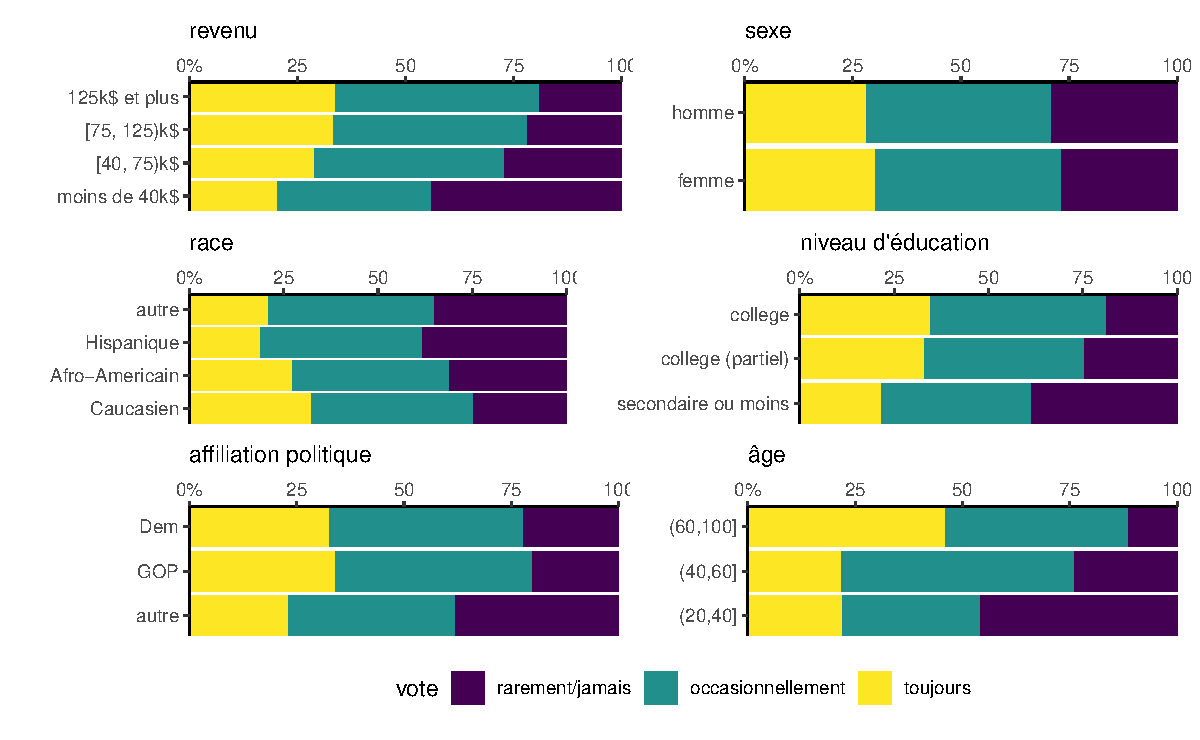
\includegraphics[width=0.9\textwidth,height=\textheight]{reglogistique_files/figure-pdf/fig-multinom_means-Ipsos-1.pdf}

}

\caption{\label{fig-multinom_means-Ipsos}Proportion des modalités des
variables sociodémographiques des données de participation électorale.}

\end{figure}%

On voit que les personnes plus fortunées, plus éduquées, plus âgées et
celles qui s'associent à un parti politique principal (Républicains et
Démocrates), votent davantage. L'écart selon l'âge est particulièrement
édifiant, avec près de 50\% des jeunes qui n'ont pas participé. Il faut
garder en tête que le revenu, l'âge et le niveau d'éducation sont
fortement associés et que les personnes plus jeunes ont eu moins
d'occasions de voter (ce qui pourrait expliquer la plus grande
propension pour les catégories de vote).

Une étude plus attentive révèle que la distribution conditionnelle de
ceux qui votent toujours est bimodale. La Figure~\ref{fig-vote-age}
montre clairement que les très jeunes et les personnes âgées en font
partie. Ainsi, le modèle est potentiellement mal spécifié car le vrai
effet de l'âge n'est visiblement pas linéaire au niveau du log de la
cote. Cela dit, les primovotant(e)s n'ont souvent eu qu'une seule
occasion de voter, ce qui peut expliquer le comportement sur le
graphique et l'absence de réponses pour occasionnellement. Pour éviter
cet artefact, on considère les personnes de plus de 30 ans uniquement.

\begin{figure}[ht!]

\centering{

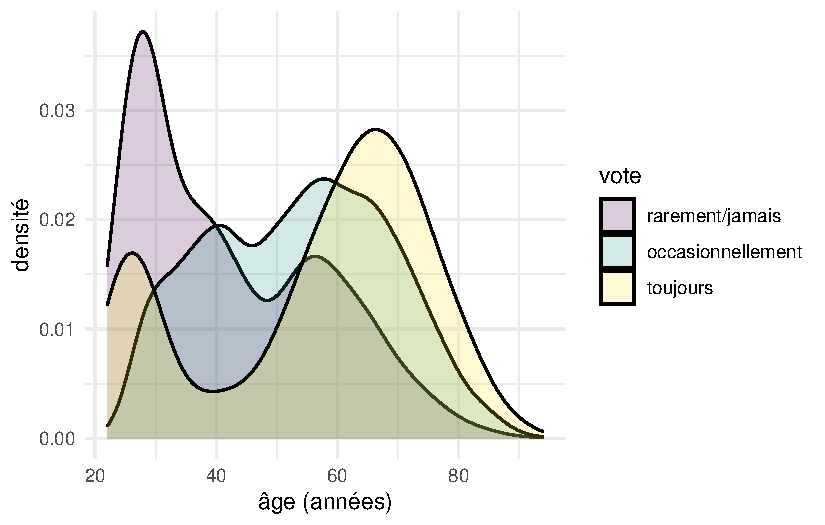
\includegraphics[width=0.85\textwidth,height=\textheight]{reglogistique_files/figure-pdf/fig-vote-age-1.pdf}

}

\caption{\label{fig-vote-age}Fréquence de vote selon l'âge.}

\end{figure}%

Pour le modèle logit multinomial, nous allons prendre
\texttt{rarement/jamais} comme catégorie de référence pour la variable
réponse \texttt{catvote}. Notez qu'il est d'usage et préférable, pour
réduire le risque de problèmes numériques et accélérer l'optimisation,
de centrer et réduire les variables explicatives.

\begin{Shaded}
\begin{Highlighting}[]
\FunctionTok{data}\NormalTok{(vote, }\AttributeTok{package =} \StringTok{"hecmulti"}\NormalTok{)}
\CommentTok{\# Modèle multinomial}
\NormalTok{multi1 }\OtherTok{\textless{}{-}}\NormalTok{ nnet}\SpecialCharTok{::}\FunctionTok{multinom}\NormalTok{(}
\NormalTok{  catvote }\SpecialCharTok{\textasciitilde{}} \FunctionTok{scale}\NormalTok{(age, }\AttributeTok{scale =} \ConstantTok{FALSE}\NormalTok{), }\CommentTok{\# centrer}
  \AttributeTok{data =}\NormalTok{ vote, }
  \AttributeTok{subset =}\NormalTok{ age }\SpecialCharTok{\textgreater{}} \DecValTok{30}\NormalTok{,}
  \AttributeTok{weights =}\NormalTok{ poids,}
  \AttributeTok{Hess =} \ConstantTok{TRUE}\NormalTok{,}
  \AttributeTok{trace =} \ConstantTok{FALSE}\NormalTok{) }
\CommentTok{\# Tableau résumé de l\textquotesingle{}ajustement}
\FunctionTok{summary}\NormalTok{(multi1)}
\CommentTok{\# Estimations des coefficients}
\FunctionTok{coef}\NormalTok{(multi1)}
\CommentTok{\# Intervalles de confiance (Wald)}
\FunctionTok{confint}\NormalTok{(multi1)}
\CommentTok{\# Critères d\textquotesingle{}information}
\FunctionTok{AIC}\NormalTok{(multi1)}
\FunctionTok{BIC}\NormalTok{(multi1)}
\CommentTok{\# Prédictions: probabilité de chaque scénario}
\FunctionTok{predict}\NormalTok{(multi1, }\AttributeTok{type =} \StringTok{"probs"}\NormalTok{)}
\CommentTok{\# Prédictions: classe la plus susceptible}
\FunctionTok{predict}\NormalTok{(multi1, }\AttributeTok{type =} \StringTok{"class"}\NormalTok{)}
\end{Highlighting}
\end{Shaded}

\begin{longtable}[]{@{}lrrr@{}}

\caption{\label{tbl-multinom-coefs}Estimation des coefficients et
intervalles de confiance à 95 pourcent pour le modèle multinomial
logistique avec les données de vote.}

\tabularnewline

\caption{catégorie rarement/jamais vs toujours}\tabularnewline
\toprule\noalign{}
& coefficient & IC (2.5\%) & IC (97.5\%) \\
\midrule\noalign{}
\endfirsthead
\toprule\noalign{}
& coefficient & IC (2.5\%) & IC (97.5\%) \\
\midrule\noalign{}
\endhead
\bottomrule\noalign{}
\endlastfoot
cst & 0.783 & 0.709 & 0.858 \\
age & 0.031 & 0.025 & 0.036 \\

\end{longtable}

\begin{longtable}[]{@{}lrrr@{}}

\caption{\label{tbl-multinom-coefs}Estimation des coefficients et
intervalles de confiance à 95 pourcent pour le modèle multinomial
logistique avec les données de vote.}

\tabularnewline

\caption{catégorie occasionnellement vs toujours}\tabularnewline
\toprule\noalign{}
& coefficient & IC (2.5\%) & IC (97.5\%) \\
\midrule\noalign{}
\endfirsthead
\toprule\noalign{}
& coefficient & IC (2.5\%) & IC (97.5\%) \\
\midrule\noalign{}
\endhead
\bottomrule\noalign{}
\endlastfoot
cst & -0.128 & -0.224 & -0.032 \\
age & 0.082 & 0.075 & 0.089 \\

\end{longtable}

Comme il y a trois catégories pour la variable dépendante, il y a deux
équations pour le modèle ajusté. En regardant les coefficients dans le
Tableau~\ref{tbl-multinom-coefs}, on obtient: \begin{align*}
\ln \left\{\frac{\Pr(\texttt{catvote}_{1i}= \texttt{occasionnellement}\mid \texttt{age}_i)}{\Pr(\texttt{catvote}_{1i} = \texttt{rarement/jamais} \mid \texttt{age}_i)} \right\} &=
0.783 + 
0.031 \texttt{age}_i, \\ 
\ln \left\{\frac{\Pr(\texttt{catvote}_{1i}= \texttt{toujours}\mid \texttt{age}_i)}{\Pr(\texttt{catvote}_{1i}= \texttt{rarement/jamais}  \mid \texttt{age}_i)} \right\} &= 
-0.128 + 0.082\texttt{age}_i. 
\end{align*}

Plus l'âge du répondant augmente, plus la probabilité que la personne
votre toujours augmente. Ainsi, la cote moyenne pour toujours versus la
référence rarement/jamais est multipliée par \(1.031=\exp(0.031)\) pour
chaque année de plus. Pour faire simple, on a employé une seule variable
explicative, mais il est clair au vu de l'analyse exploratoire que
d'autres variables sont utiles pour comprendre le comportement des
électeurs et électrices. Qui est plus, la taille de la base de données
nous permettrait de mesurer d'autres effets.

On peut comparer les modèles emboîtés à l'aide de tests de rapport de
vraisemblance.

\begin{Shaded}
\begin{Highlighting}[]
\CommentTok{\# Ajuster modèle sous H0: les}
\CommentTok{\# prédictions correspondent à la}
\CommentTok{\# proportion empirique de chaque catégorie}
\NormalTok{multi0 }\OtherTok{\textless{}{-}}\NormalTok{ nnet}\SpecialCharTok{::}\FunctionTok{multinom}\NormalTok{(catvote }\SpecialCharTok{\textasciitilde{}} \DecValTok{1}\NormalTok{,}
                         \AttributeTok{weights =}\NormalTok{ poids,}
                         \AttributeTok{data =}\NormalTok{ vote,}
                         \AttributeTok{subset =}\NormalTok{ age }\SpecialCharTok{\textgreater{}} \DecValTok{30}\NormalTok{,}
                         \AttributeTok{trace =} \ConstantTok{FALSE}\NormalTok{)}
\CommentTok{\# Test de rapport de vraisemblance}
\FunctionTok{anova}\NormalTok{(multi0, multi1)}
\end{Highlighting}
\end{Shaded}

\begin{longtable}[]{@{}lrrrrl@{}}

\caption{\label{tbl-anova-multinom}Analyse de déviance: test du rapport
de vraisemblance pour la variable explicative dans le modèle multinomial
logistique.}

\tabularnewline

\toprule\noalign{}
modèle & DL & déviance & DL & rapport vrais. & valeur-p \\
\midrule\noalign{}
\endhead
\bottomrule\noalign{}
\endlastfoot
cst & 9692 & 9781 & & & \\
age & 9690 & 9078 & 2 & 703 & \textless0.0001 \\

\end{longtable}

Cette valeur est donnée dans la dernière colonne du tableau. De plus,
cet effet est significatif car la valeur-\(p\) est inférieure à
\(10^{-4}\).

Pour une comparaison directe entre les deux autres catégories,
\texttt{rarement/jamais} et \texttt{occasionnellement}, il suffit de
changer la catégorie de référence.

\subsection{Régression logistique cumulative à cotes
proportionnelles}\label{ruxe9gression-logistique-cumulative-uxe0-cotes-proportionnelles}

Si les modalités de la réponse sont ordinales, la régression logistique
multinomiale est toujours appropriée. Il peut néanmoins être préférable
d'utiliser un modèle qui utilise l'ordre des modalités pour obtenir un
modèle plus facile à interpréter et plus parcimonieux. Le modèle de
régression logistique cumulative à cotes proportionnelles
(\citeproc{ref-McCullagh:1980}{McCullagh 1980}) est une simplification
du modèle multinomial sous l'hypothèse que les rapports de cotes sont
les mêmes peut importe la catégorie.

Supposons que les \(K\) modalités de la variable \textbf{ordinale} \(Y\)
sont en ordre croissant et que l'on dispose de \(p\) variables
explicatives \(\mathrm{X}_1, \ldots, \mathrm{X}_p\) pour chaque
observation. Soit \(p_{ik}=\Pr(Y_i=k \mid \mathbf{X}_{i})\)
(\(k=1, \ldots, K\)) la probabilité que \(Y_{i}\) prenne la valeur
\(k\).

Le modèle logistique à cotes proportionnelles spécifie que pour
\(k=1, \ldots, K-1\), \begin{align*}
\frac{\Pr(Y_i > k \mid \mathbf{X}_i)}{\Pr(Y_i \leq k \mid \mathbf{X}_i)} = \frac{p_{i(k+1)} + \cdots + p_{iK}}{p_{i1} + \cdots + p_{ik}} = \exp(\mathbf{X}_i \boldsymbol{\beta} - \zeta_k),
\end{align*} en utilisant la paramétrisation de la fonction
\texttt{polr} du paquet \texttt{MASS}. Le terme \(-\eta_{k}\) correspond
à l'ordonnée à l'origine spécifique à la catégorie \(k\) et
\(-\infty=\zeta_0 < \zeta_1 < \cdots < \zeta_K =\infty\) aux points de
coupe qui déterminent les probabilités de chaque catégorie. Puisque
\(\Pr(Y_i > K \mid \mathbf{X}_i)=1\), il y a \(K-1\) équations pour le
rapport de cote. Si l'ordonnée à l'origine change d'une équation à
l'autre, les paramètres quantifiant les effets des variables
explicatives, \(\beta_1, \ldots, \beta_p\) sont les mêmes pour chacune
des cotes. Par conséquent, pour modéliser une variable ordinale \(Y\)
ayant \(K\) valeurs possibles et avec \(p\) variables explicatives, le
modèle cumulatif logistique utilise \(p + K - 1\) paramètres. Le modèle
logit multinomial, qui peut également être utilisé pour les données
ordinales, utilise plutôt \((K-1) \cdot(p+1)\) paramètres. Le modèle
logistique cumulatif à cotes proportionnelles est donc plus parcimonieux
et, pour autant qu'il soit approprié, mènera à des estimations des
paramètres plus précises qu'avec le modèle de régression logistique
multinomiale. Les deux modèles sont identiques au modèle de régression
logistique si la variable ordinale a uniquement deux modalités (variable
binaire).

La cote pour \(Y_i > k\) mesure à quel point il est plus probable que
\(Y_i\) prenne une valeur plus grande que \(k\) par rapport à une valeur
plus petite ou égale à \(k\). Dans cet exemple, nous n'avons aucune
transformation des variables explicatives, ni aucune interaction dans le
modèle; l'interprétation des paramètres est donc simplifiée. Si le
paramètre \(\beta_j\) est positif, cela indique que plus
\(\mathrm{X}_j\) prend une valeur élevée, plus la variable \(Y\) a
tendance à prendre aussi une valeur élevée. Inversement, si le paramètre
\(\beta_j\) est négatif, cela indique que plus \(\mathrm{X}_j\) prend
une valeur élevée, plus la variable \(Y\) a tendance à prendre une
valeur basse. Plus précisément, pour chaque augmentation d'une unité de
\(\mathrm{X}_j\), la cote pour \(\Pr(Y_i > k \mid \mathbf{X}_i)\) versus
\(\Pr(Y_i \leq k \mid \mathbf{X}_i)\) est multipliée par
\(\exp(\beta_j)\), peu importe la valeur de \(Y\). En terme de
probabilité cumulée d'excéder \(k\), \begin{align*}
\Pr(Y_i > k \mid \mathbf{X}_i) &= \textrm{expit}(-\eta_k + \beta_1 \mathrm{X}_{i1} + \cdots + \beta_p \mathrm{X}_{ip}), \qquad k=1, \ldots, K-1.
\end{align*} En utilisant ces expressions, on peut obtenir la
probabilité de chaque catégorie, \begin{align*}
&\Pr(Y_i = k \mid \mathbf{X}_{i}) =\Pr(Y_i > k \mid \mathbf{X}_{i}) - \Pr(Y_i > k-1 \mid \mathbf{X}_{i}).
\end{align*}

On peut répéter le même modèle que précédemment pour les données de
sondage, même s'il est peu susceptible que l'hypothèse de cotes
proportionnelles soit valide. Dans \textbf{R}, la variable réponse doit
être de classe \texttt{ordered}, une forme particulière de facteur dont
les niveaux sont ordonnés en ordre croissant. On ajuste un modèle, cette
fois avec sexe pour nous permettre de pratiquer l'interprétation d'une
variable catégorielle.

\begin{Shaded}
\begin{Highlighting}[]
\CommentTok{\# Modèle de régression logistique }
\CommentTok{\# multinomiale ordinale à cote proportionnelle}
\FunctionTok{with}\NormalTok{(vote, }\FunctionTok{is.ordered}\NormalTok{(catvote))}
\NormalTok{multi2a }\OtherTok{\textless{}{-}}\NormalTok{ MASS}\SpecialCharTok{::}\FunctionTok{polr}\NormalTok{(}
\NormalTok{  catvote }\SpecialCharTok{\textasciitilde{}}\NormalTok{ sexe, }
  \AttributeTok{data =}\NormalTok{ vote, }
  \AttributeTok{subset =}\NormalTok{ age }\SpecialCharTok{\textgreater{}} \DecValTok{30}\NormalTok{,}
  \AttributeTok{weights =}\NormalTok{ poids,}
  \AttributeTok{method =} \StringTok{"logistic"}\NormalTok{, }
  \AttributeTok{Hess =} \ConstantTok{TRUE}\NormalTok{)}

\NormalTok{multi2b }\OtherTok{\textless{}{-}}\NormalTok{ nnet}\SpecialCharTok{::}\FunctionTok{multinom}\NormalTok{(}
\NormalTok{  catvote }\SpecialCharTok{\textasciitilde{}}\NormalTok{ sexe, }
  \AttributeTok{data =}\NormalTok{ vote,}
  \AttributeTok{subset =}\NormalTok{ age }\SpecialCharTok{\textgreater{}} \DecValTok{30}\NormalTok{, }
  \AttributeTok{weights =}\NormalTok{ poids,}
  \AttributeTok{Hess =} \ConstantTok{TRUE}\NormalTok{,}
  \AttributeTok{trace =} \ConstantTok{FALSE}\NormalTok{)}
\CommentTok{\# Le modèle est paramétré en terme}
\CommentTok{\#  du rapport de cote, ascendant}
\FunctionTok{summary}\NormalTok{(multi2a)}
\CommentTok{\# Test du rapport de vraisemblance pour }
\CommentTok{\# modèle à cote proportionnelle}
\CommentTok{\# deviance = {-}2*ll}
\FunctionTok{pchisq}\NormalTok{(}\FunctionTok{deviance}\NormalTok{(multi2a) }\SpecialCharTok{{-}} \FunctionTok{deviance}\NormalTok{(multi2b),}
       \AttributeTok{df =} \FunctionTok{length}\NormalTok{(}\FunctionTok{coef}\NormalTok{(multi2a)), }
       \AttributeTok{lower.tail =} \ConstantTok{FALSE}\NormalTok{)}
\CommentTok{\# Intervalles de confiance pour beta\_x}
\CommentTok{\#  {-} vraisemblance profilée}
\FunctionTok{confint}\NormalTok{(multi2a)}
\CommentTok{\# Critères d\textquotesingle{}information}
\FunctionTok{AIC}\NormalTok{(multi2a)}
\FunctionTok{BIC}\NormalTok{(multi2a)}

\CommentTok{\# Tableau des coefficients }
\CommentTok{\# Négatif de l\textquotesingle{}ordonnée à l\textquotesingle{}origine:}
\NormalTok{multi2a}\SpecialCharTok{$}\NormalTok{zeta}
\CommentTok{\# Uniquement pour variables explicatives}
\CommentTok{\# exp(beta) avec l\textquotesingle{}IC de vraisemblance profilée}
\FunctionTok{exp}\NormalTok{(}\FunctionTok{c}\NormalTok{(}\FunctionTok{coef}\NormalTok{(multi2a), }\FunctionTok{confint}\NormalTok{(multi2a)))}
\CommentTok{\# On peut obtenir les intervalles de Wald }
\CommentTok{\# avec confint.default}

\CommentTok{\# Test d\textquotesingle{}adéquation }
\CommentTok{\# (rapport de vraisemblance, comparaison avec modèle saturé)}
\FunctionTok{pchisq}\NormalTok{(}\AttributeTok{q =} \FunctionTok{deviance}\NormalTok{(multi2a),}
       \AttributeTok{df =} \FunctionTok{df.residual}\NormalTok{(multi2a),}
       \AttributeTok{lower.tail =} \ConstantTok{FALSE}\NormalTok{)}
\CommentTok{\# Petite valeur{-}p = modèle inadéquat}
\end{Highlighting}
\end{Shaded}

\begin{table}

\caption{\label{tbl-ordered-logistic}Tableau des estimations des
coefficients du modèle pour réponses ordinales pour la régression
logistique à cotes proportionnelles avec sexe.}

\centering{

\begin{tabular}[t]{lrr}
\toprule
effet & coefficient & erreur-type\\
\midrule
sexe [homme] & -0.166 & 0.055\\
cst [rarement/jamais|occasionnellement] & -1.297 & 0.044\\
cst [occasionnellement|toujours] & 0.865 & 0.041\\
\bottomrule
\end{tabular}

}

\end{table}%

Si on écrit les équations pour la cote, on obtient \begin{align*}
\frac{\Pr(Y = \texttt{rarement} \mid \texttt{sexe})}{\Pr(Y \geq \texttt{occasionnellement} \mid \texttt{sexe})} &= \exp(-0.166\texttt{sexe} + 1.297) \\ 
\frac{\Pr(Y \leq \texttt{occasionnellement} \mid \texttt{sexe})}{\Pr(Y = \texttt{toujours} \mid \texttt{sexe})} &= \exp(-0.166\texttt{sexe} - 0.865).
\end{align*}

Ici, l'effet estimé d'être un homme plutôt qu'une femme (\texttt{sexe})
est \(-0.166\) et ce paramètre est significativement différent de zéro
(valeur-\(p\) de \(0.003\) obtenue en faisant un test de rapport de
vraisemblance).

Ainsi, les hommes sont moins susceptibles de voter fréquemment que les
femmes. Plus précisément, la cote d'être dans une catégorie plus élevée
de \texttt{catvote}, par rapport à une catégorie plus basse, est
multipliée par \(\exp(-0.166) = 0.847\), ce qui correspond à une
diminution de la cote \(15\)\% (et donc la probabilité estimée que la
personne vote plus fréquemment est plus faible).

Considérons pour illustrer le rôle des paramètres
\(\zeta_1, \ldots, \zeta_{k-1}\) pour la prédiction pour une femme
(valeur de la référence). Soit \(p_1\), \(p_2\) et \(p_3\) les
probabilités pour respectivement rarement/jamais, occasionnellement et
toujours. On peut calculer \(\mathrm{expit}(\zeta_k)\)
(\(k=0, \ldots, K\)) qui donne \(0\), \(0.215\), \(0.704\) et \(1\) et
les différences donnent \(\widehat{p}_1 = 0.215\),
\(\widehat{p}_2 = 0.489\) et \(\widehat{p}_3 = 0.296\). Un rapide calcul
numérique montre que c'est bien ce que retourne les prédictions dans le
Tableau~\ref{tbl-predpolr}.

\begin{Shaded}
\begin{Highlighting}[]
\FunctionTok{predict}\NormalTok{(multi2a, }
        \AttributeTok{newdata =} \FunctionTok{data.frame}\NormalTok{(}\AttributeTok{sexe =} \FunctionTok{factor}\NormalTok{(}\StringTok{"femme"}\NormalTok{)), }
        \AttributeTok{type =} \StringTok{"probs"}\NormalTok{)}
\end{Highlighting}
\end{Shaded}

\begin{longtable}[]{@{}rrr@{}}

\caption{\label{tbl-predpolr}Probabilités de chaque classe pour une
femme avec le modèle à cotes proportionnelles qui inclut uniquement le
sexe.}

\tabularnewline

\toprule\noalign{}
rarement/jamais & occasionnellement & toujours \\
\midrule\noalign{}
\endhead
\bottomrule\noalign{}
\endlastfoot
0.215 & 0.489 & 0.296 \\

\end{longtable}

Avant toute chose, il faut s'assurer que le modèle est approprié.
Rappelez-vous que l'une des hypothèses de ce modèle est que les effets
des variables explicatives sont les mêmes pour chaque équation.

\begin{itemize}
\tightlist
\item
  \(\mathscr{H}_0\) : l'effet de chaque variable est le même pour les
  \(K\) logit du modèle multinomial logistique, soit
  \(\beta_{11} = \cdots =\beta_{1K}\), \(\ldots\),
  \(\beta_{p1} = \cdots =\beta_{pK}\).
\end{itemize}

Une très petite valeur-\(p\) (rejet de \(\mathscr{H}_0\)) pour ce test
serait une indication que le modèle de régression multinomiale ordinale
n'est pas approprié et que le modèle multinomial logistique serait
préférable. Comme la valeur-\(p\) est négligeable, on rejette pas
\(\mathscr{H}_0\) et l'hypothèse de cote proportionnelle ne tient pas la
route.

\begin{figure}[ht!]

\centering{

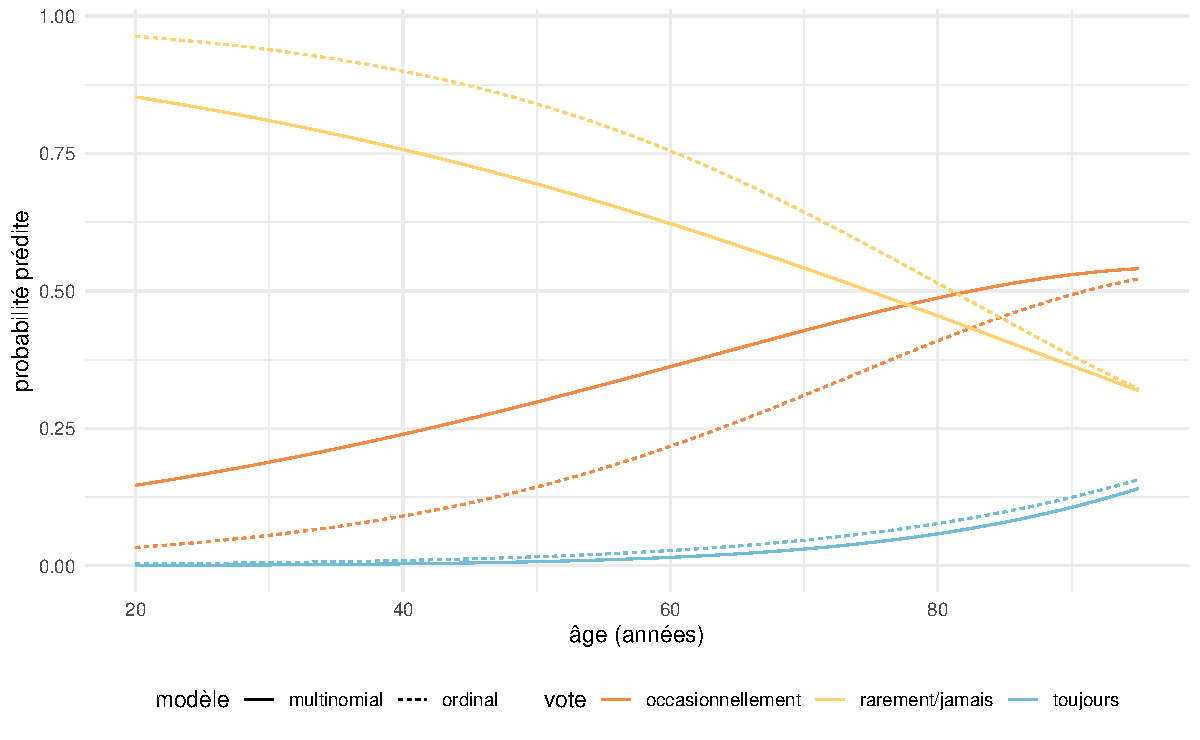
\includegraphics[width=0.85\textwidth,height=\textheight]{reglogistique_files/figure-pdf/fig-predmultinom-1.pdf}

}

\caption{\label{fig-predmultinom}Probabilités prédites pour chaque
modalité selon le modèle de régression multinomiale logistique et le
modèle de régression ordinales à cotes proportionnelles selon l'âge.}

\end{figure}%

On a précédemment utilisé un test du rapport de vraisemblance pour
valider l'hypothèse des cotes proportionnelles: il n'y avait aucune
indication que la simplification n'était pas adéquate. Ce n'est pas le
cas pour le modèle qui ne contient que la variable \texttt{age} ou
plusieurs variables explicatives: la Figure~\ref{fig-predmultinom}
montre les différences de probabilités ajustées pour les deux modèles
qui incluent uniquement l'âge comme variable explicative. Règle
générale, on n'ajustera jamais un modèle avec une seule des variables:
un test du rapport de vraisemblance indique que \textbf{toutes} les
variables explicatives sont utiles pour expliquer le comportement.

On peut également vérifier si le modèle est adéquat pour décrire les
données en comparant le modèle pour les données ordinales avec un modèle
saturé (qui contient autant de paramètres que d'observations/niveaux):
la valeur-\(p\), infime, indique que le modèle plus complexe, soit le
modèle saturé, est préférable. Cela nous indique que le modèle a un
piètre pouvoir explicatif.

\begin{tcolorbox}[enhanced jigsaw, bottomrule=.15mm, toptitle=1mm, opacityback=0, title=\textcolor{quarto-callout-note-color}{\faInfo}\hspace{0.5em}{En résumé}, left=2mm, bottomtitle=1mm, colbacktitle=quarto-callout-note-color!10!white, colback=white, breakable, toprule=.15mm, coltitle=black, arc=.35mm, opacitybacktitle=0.6, colframe=quarto-callout-note-color-frame, titlerule=0mm, leftrule=.75mm, rightrule=.15mm]

\begin{itemize}
\tightlist
\item
  La régression multinomiale logistique pour une variable catégorielle à
  \(K\) niveaux est une extension directe de la régression logistique
  pour données binaires: il y a \(K-1\) équations de cote en termes des
  variables explicatives (puisque la somme des probabilités vaut 1),
  donc le nombre de paramètres croît rapidement.
\item
  Le modèle est multiplicatif: la cote de catégorie \(k\) vs référence
  est multipliée par \(\exp(\beta_{jk})\) pour chaque augmentation de
  \(\mathrm{X}_j\) d'une unité.
\item
  Les coefficients manquants de la sortie du tableau peuvent être
  déduits par des manipulations algébriques.
\item
  Le modèle cumulatif à cote proportionnelle est une simplification du
  modèle multinomial pour des données ordinales.
\item
  On suppose que l'effet des variables est le même pour la cote de la
  survie de chaque modalité
\item
  Le modèle à cotes proportionnelles a moins de paramètres, mais le
  postulat de cotes proportionnelles doit être vérifié (via un test de
  rapport de vraisemblance ou un test du score).
\end{itemize}

\end{tcolorbox}

\bookmarksetup{startatroot}

\chapter{Analyse de survie}\label{analyse-survie}

\section{Introduction}\label{introduction-2}

Cette section traite de temps avant qu'un événement survienne. Le
traitement de ce type de données, dites données de survie en référence
au domaine médical, est particulier parce que l'information disponible
est incomplète. Plusieurs mécanismes peuvent impacter la survie:
généralement les données sont sujettes à troncature et à censure.

Pour déterminer les mécanismes de survie en présence, il peut être utile
de représenter le processus de collecte de données à l'aide d'un
diagramme de Lexis: ce dernier présente la trajectoire observée à l'aide
d'une droite de pente un. L'axe des abscisses (\(x\)) donne le temps (au
calendrier) et l'axe des ordonnées (\(y\)) la durée observée.

\begin{figure}[ht!]

\centering{

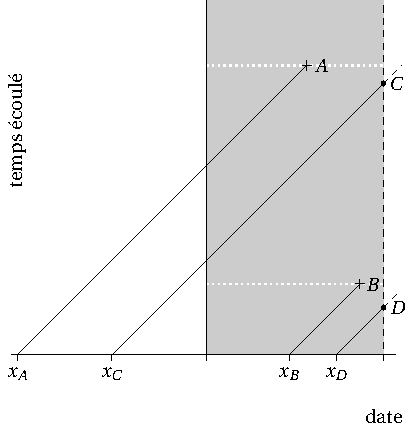
\includegraphics[width=0.55\textwidth,height=\textheight]{figures/Lexis_censure.pdf}

}

\caption{\label{fig-lexis}Diagramme de Lexis pour données tronquées à
gauche (\(A\) et \(C\)) et censurées à droite (\(C\) et \(D\)).}

\end{figure}%

La Figure~\ref{fig-lexis} montre des courbes fictives. On trace une
droite de pente 1 représentant la durée en fonction du temps (date au
calendrier) et la fenêtre définit la période de collecte de donnée. La
censure est indiquée par des cercles, les événements par des croix.

On parle de censure lorsque le temps réel de l'événement n'est pas
observé (information partielle).

\begin{itemize}
\tightlist
\item
  Censure à droite: l'événement n'est pas encore survenu au temps \(t\):
  on sait que \(T > t\).
\item
  Censure à gauche: l'événement survient avant le temps \(t\), donc la
  vraie valeur est inférieure à la valeur observée (\(T < t\))
\item
  Censure par intervalle: l'événement est survenu dans la plage
  \([t_1, t_2]\) (données arrondies)
\end{itemize}

La censure peut être aléatoire (par exemple, une personne qui fait
partie d'un protocole de rercherche déménage dans un autre pays parce
que sa conjointe a trouvé un emploi là-bas et cette raison n'a aucun
lien avec son état de santé). La censure administrative, un mécanisme
déterministe qui survient lorsque les données sont collectées sur une
période fixe de temps, ne fournit pas non plus d'information sur
l'événement en question. On supposera dans ces notes que nous sommes
dans un de ces deux cas de figure.

Si la censure est informative, les outils présentés ne sont pas
adéquats! Par exemple, si un patient d'une étude clinique est déchargé
d'un protocole médical car il est trop mal en point, cela nous renseigne
sur son état de santé et sur sa survie.

La troncature, rarement discutée, est liée au processus de collecte et
détermine quelles observations sont incluses dans l'étude. La plage des
valeurs possibles est tronquée. Les types de troncature sont:

\begin{itemize}
\tightlist
\item
  troncature à gauche: le temps minimum est supérieur à \(t_0\)
\item
  troncature à droite: le temps maximum est inférieur à \(t_1\)
\item
  troncature par intervalle: le temps de l'événement doit survenir entre
  \(t_0\) et \(t_1\).
\end{itemize}

La troncature à gauche est la plus fréquente: elle survient par exemple
si on étudie le temps d'abonnement, mais qu'on n'a accès qu'aux dossiers
de clients et de clientes qui sont actifs dans le système. Ainsi, une
personne qui se serait désabonnée une journée avant qu'on télécharge les
données ne se trouvera pas dans la base de données. Si on ne tient pas
compte de cet état de fait et des fantômes, nos estimations seront
biaisées.

La troncature par intervalle survient quand on considère uniquement les
personnes pour lesquelles l'événement d'intérêt est survenu. Si l'on
s'intéresse à la durée de la relation d'emploi et seules les personnes à
l'emploi qui ont pris leur retraite entre 2009 et 2021 sont considérées
pour l'étude, on sera en présence de troncature par intervalle comme
représenté dans la Figure~\ref{fig-troncatureintervalle}.

\begin{figure}[ht!]

\centering{

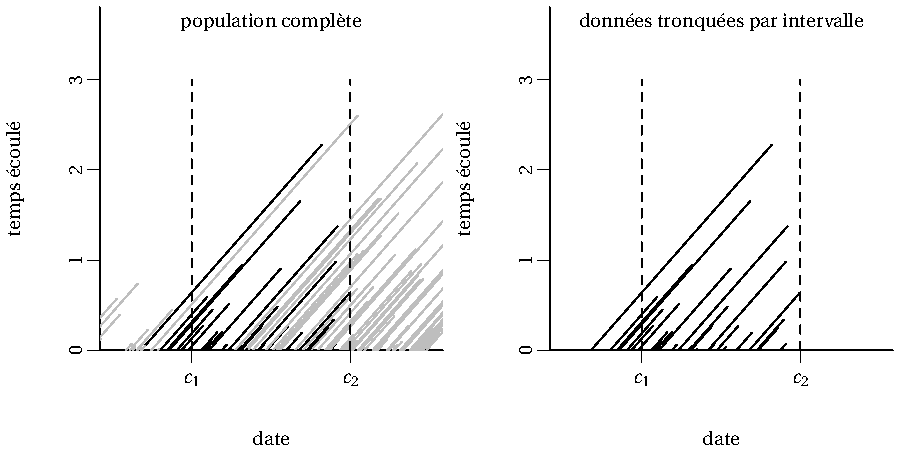
\includegraphics[width=1\textwidth,height=\textheight]{figures/lexis_troncationintervalle.pdf}

}

\caption{\label{fig-troncatureintervalle}Diagramme de Lexis illustrant
la troncature par intervalle.}

\end{figure}%

On considère comme exemple une étude sur le chômage dû à la crise du
coronavirus. On s'intéresse à tous ceux qui étaient en recherche active
d'emploi entre mars et juin; seuls ceux qui étaient au chômage durant
cette période seront considérés. Certaines personnes seront déjà au
chômage en avril et donc leur durée de chômage en mars est déjà longue
(troncature à gauche). Lors de notre suivi, d'autres personnes
mentionneront avoir trouvé un emploi lors de notre appel, mais ne
pourront nous renseigner sur la date exacte de leur embauche: cette
dernière précèdera notre prise de contact, mais nous est inconnue
(censure à gauche). D'autres personnes seront toujours au chômage en
juin à la fin de l'étude et on ignorera le nombre réel de mois passés au
chômage (censure à droite). Enfin, certaines personnes cesseront de
chercher activement un emploi et donc quitteront l'étude (censure à
droite). Tous ces méchanismes (complexes) peuvent être dictés par
certaines covariables (employabilité, découragement) et être aléatoires
ou pas. Pour estimer le taux de chômage, il faudra prendre en compte les
méchanismes de survie dans notre modèle. On se concentrera sur le cas
simple des données censurées à droite de façon aléatoire.

Avec la survie, les statistiques descriptives usuelles sont trompeuses.
La figure de
\href{https://theconversation.com/music-to-die-for-how-genre-affects-popular-musicians-life-expectancy-36660}{cet
article tiré de \emph{The Conversation}} montre l'impact drastique de la
censure en représentant l'âge moyen au décès en fonction du genre
musical, ordonné par ordre d'apparition de ce dernier. Puisque seules
les personnes décédées sont incluses, les artistes de hip-hop décédés
l'ont été forcément en bas-âge. Si on ne prend pas en compte la censure,
on obtiendrait une conclusion erronnée.

\subsection{Exemple du temps
d'abonnement}\label{exemple-du-temps-dabonnement}

Une entreprise oeuvrant dans le secteur des télécommunications
s'intéresse aux facteurs influençant le temps qu'un client reste abonné
à son service de téléphone cellulaire. Des données provenant d'un
échantillon de clients se trouvent dans le fichier \texttt{survie1}, qui
contient les variables suivantes:

\begin{itemize}
\tightlist
\item
  \(\texttt{temps}\): temps (en semaines) que le client est resté abonné
  au service de téléphone cellulaire. Il s'agit du vrai temps si le
  client n'est plus abonné et d'un temps censuré à droite si le client
  est toujours abonné.
\item
  \(\texttt{censure}\): variable binaire qui indique si la variable
  \(\texttt{t}\) est censurée (\(0\) si le client est toujours abonné)
  ou non (\(1\), la variable \(\texttt{t}\) est la durée finale de
  l'abonnement).
\item
  \(\texttt{age}\): âge du client au début de l'abonnement.
\item
  \(\texttt{sexe}\): sexe du client, soit femme (\(1\)), soit homme
  (\(0\)).
\item
  \(\texttt{service}\): nombre de services en plus du cellulaire auquel
  le client est abonné parmi internet, téléphone fixe, télévision (câble
  ou antenne parabolique).
\item
  \(\texttt{region}\): région où habite le client en ce moment (valeurs
  entre 1 et 5).
\end{itemize}

\subsection{Contexte}\label{contexte}

On s'intéresse au temps avant qu'un événement survienne. On observe
chaque sujet jusqu'à ce que l'une des deux choses suivantes se produise
: l'événement survient avant la fin de la période d'observation ou bien
l'étude se termine et l'événement n'est toujours pas survenu. Dans
l'exemple, l'événement correspond au fait d'interrompre son abonnement.
On dispose donc d'une variable « temps », que l'on nomme \(T\), pour
chaque individu qui est soit censurée soit non censurée. Si l'individu a
expérimenté l'événement avant la fin de la période d'observation, la
valeur de \(T\) n'est pas censurée. Si l'événement n'est toujours pas
survenu à la fin de la période d'observation, la valeur de \(T\) est
censurée. Pour chaque individu, on dispose également d'un ensemble de
variables explicatives \(X_1, \ldots, X_p\). Pour l'instant, supposons
que les valeurs de ces variables sont fixes dans le temps mais on
reviendra plus loin au cas où leurs valeurs peuvent varier dans le
temps. Bien que le terme analyse de survie semble implicitement référer
à la santé, de nombreux autres exemples sont envisageables

\begin{itemize}
\tightlist
\item
  temps qu'un client demeure abonné à un service offert par notre
  compagnie.
\item
  temps de survie d'un individu après avoir été diagnostiqué avec un
  certain type de cancer.
\item
  ancienneté d'un travailleur au service d'une compagnie.
\item
  durée de vie d'une franchise.
\item
  temps avant la faillite d'une entreprise (ou d'un particulier).
\item
  temps avant le prochain achat d'un client.
\item
  temps durant lequel un(e) employé(e) est au chômage.
\end{itemize}

Si aucune observation n'est censurée, c'est-à-dire, si on a observé le «
vrai » temps pour chaque sujet, on pourrait alors simplement modéliser
\(T\) en incluant des covariables dans les paramètres de vraisemblance
d'une loi positive (par exemple, avec une régression log-linéaire). En
revanche, si des observations sont censurées dans l'échantillon, leur
omission biaiserait l'analyse.

Ce chapitre se veut une introduction à l'analyse de données de survie.
Comme le développement de la théorie de l'analyse de survie est assez
complexe (plus encore que celle de la régression linéaire ou
logistique), on s'intéressera ici uniquement aux principes de base afin
d'être en mesure d'appliquer les méthodes et de bien interpréter les
résultats. Plusieurs extensions sont également possibles. Un survol de
ces dernières sera effectué dans des sections plus loin.

Il existe deux grandes approches pour analyser des données de survies :

\begin{enumerate}
\def\labelenumi{\roman{enumi})}
\tightlist
\item
  nonparamétrique ou semi-paramétrique: estimateur de Kaplan--Meier,
  modèle de Cox (à risques proportionnels).
\item
  paramétrique : modèle paramétrique avec loi continue (Weibull,
  log-normal, log-logistique, gamma).
\end{enumerate}

Nous discuterons seulement de la première approche dans ce chapitre. Le
tableau suivant fait une analogie entre ce que nous ferons dans ce
chapitre et des méthodes que vous connaissez.

\begin{longtable}[]{@{}
  >{\raggedright\arraybackslash}p{(\columnwidth - 6\tabcolsep) * \real{0.2323}}
  >{\raggedright\arraybackslash}p{(\columnwidth - 6\tabcolsep) * \real{0.2839}}
  >{\raggedright\arraybackslash}p{(\columnwidth - 6\tabcolsep) * \real{0.3355}}
  >{\raggedright\arraybackslash}p{(\columnwidth - 6\tabcolsep) * \real{0.1484}}@{}}
\toprule\noalign{}
\begin{minipage}[b]{\linewidth}\raggedright
réponse \(Y\)
\end{minipage} & \begin{minipage}[b]{\linewidth}\raggedright
résumé descriptif
\end{minipage} & \begin{minipage}[b]{\linewidth}\raggedright
comparaison de deux groupes
\end{minipage} & \begin{minipage}[b]{\linewidth}\raggedright
modèle général
\end{minipage} \\
\midrule\noalign{}
\endhead
\bottomrule\noalign{}
\endlastfoot
continue & moyenne & test-\(t\) pour deux échantillons & régression
linéaire \\
binaire & proportion & test d'indépendance du khi-deux & régression
logistique \\
temps de survie (censure à droite) & fonction de survie temps de survie
médian & test log-rang test de Wilcoxon généralisé (Gehan) & modèle de
Cox \\
\end{longtable}

La structure de données de base que l'on doit avoir pour travailler est
la suivante:

\begin{enumerate}
\def\labelenumi{\arabic{enumi})}
\tightlist
\item
  une variable temps, \(T\).
\item
  une variable binaire \(C\) (censure).
\item
  d'autres variables explicatives \(X_1, \ldots, X_p\), une par colonne.
\end{enumerate}

\section{Fonctions de survie et de
risque}\label{fonctions-de-survie-et-de-risque}

Un des éléments de base d'une analyse de survie (\emph{survival
analysis}) est la \textbf{fonction (ou courbe) de survie}. Soit
\(F(t)=\Pr(T \leq t)\) la fonction de répartition du temps de survie
\(t\) et \(f(t) = \mathrm{d} / \mathrm{d} t F(t)\). La fonction de
survie est \begin{align*}
S(t)= \Pr(T > t) = 1-F(t)
\end{align*} et donne la probabilité que le temps de survie soit
supérieur à \(t\). On verra plus loin comment estimer cette fonction
avec un échantillon et comment tester l'égalité de deux (ou plusieurs)
fonctions de survie.

La \textbf{fonction de risque} (en anglais, \emph{hazard}) est
\begin{align*}
h(t) =  \frac{f(t)}{S(t)}
\end{align*} où \(f(t)\) est la fonction de densité (pour \(T\) continu)
ou de masse pour \(T\) discret. Dans le cas discret où le temps peut
seulement prendre les valeurs \(0, 1, 2, \ldots\), la fonction de risque
est donc simplement la probabilité que l'événement survienne au temps
\(t\), étant donné qu'il n'était pas survenu avant, \begin{align*}
\Pr(T=t \mid T > t) = \Pr(T=t) / \Pr(T >t) = f(t)/S(t);
\end{align*} c'est une probabilité conditionnelle. Dans le cas général,
la fonction de risque est nécessairement positive mais peut prendre des
valeurs supérieures à un. On ne peut donc pas, à strictement parler, la
voir comme une probabilité et c'est pourquoi on parle plutôt de risque.
En fait, cette fonction mesure le risque instantané que l'événement
survienne au temps \(t\), étant donné qu'il n'était pas survenu avant.

Cette fonction est importante car il s'agit de celle que nous allons
modéliser avec le modèle de régression de Cox. Si, en régression
logistique, on modélise le logarithme des cotes, on modélise plutôt la
fonction de risque en analyse de survie. Les fonctions de survie et de
risque sont intimement reliées et \begin{align*}
h(t) = - \frac{\mathrm{d} \ln\{S(t)\}}{\mathrm{d} t}, \qquad \qquad S(t) = \exp \left\{ -\int_0^t h(u) \mathrm{d} u\right\}.
\end{align*} Ainsi, si on connaît la fonction de survie, on peut
retrouver la fonction de risque et vice-versa. Par conséquent, un modèle
pour la fonction de survie spécifie une fonction de risque (et
vice-versa).

\section{Estimation d'une courbe de survie et de
risque}\label{estimation-dune-courbe-de-survie-et-de-risque}

L'estimateur nonparamétrique le plus couramment utilisé pour
l'estimation de la fonction de survie en présense de censure à droite
est l'estimateur de Kaplan--Meier. De plus, cette méthode est
nonparamétrique en ce sens qu'on ne suppose aucun modèle et qu'on
suppose uniquement que la censure est non-informative.

Si l'échantillon ne contient aucune observation censurée (on a des temps
exacts pour tous les sujets), l'estimateur de Kaplan--Meier de la
fonction de survie à un temps \(t\) donné est alors simplement la
proportion des observations dans l'échantillon qui possède un temps de
survie supérieur à \(t\). Par convention, on considère qu'une
observation censurée à droite faisait partie de l'ensemble
d'observations à risque au temps de censure observé.

On considère l'exemple des temps d'abonnement pour illustrer le concept.
L'estimation de la fonction de survie selon la méthode Kaplan--Meier est
obtenue grâce aux commandes suivantes:

\begin{Shaded}
\begin{Highlighting}[]
\FunctionTok{library}\NormalTok{(survival)}
\FunctionTok{data}\NormalTok{(survie1, }\AttributeTok{package =} \StringTok{"hecmulti"}\NormalTok{)}
\CommentTok{\# Estimateur de Kaplan{-}Meier}
\CommentTok{\# La réponse "temps"est le temps de survie }
\CommentTok{\# et l\textquotesingle{}indicateur de censure "censure" est}
\CommentTok{\# "0" pour censuré à droite, "1" pour événement}
\NormalTok{kapm }\OtherTok{\textless{}{-}} 
  \FunctionTok{survfit}\NormalTok{(}\FunctionTok{Surv}\NormalTok{(temps, censure) }\SpecialCharTok{\textasciitilde{}} \DecValTok{1}\NormalTok{, }
          \AttributeTok{conf.type =} \StringTok{"log"}\NormalTok{, }
          \AttributeTok{data =}\NormalTok{ survie1)}
\FunctionTok{summary}\NormalTok{(kapm)}
\FunctionTok{quantile}\NormalTok{(kapm)}
\FunctionTok{plot}\NormalTok{(kapm, }
     \AttributeTok{ylab =} \StringTok{"fonction de survie"}\NormalTok{, }
     \AttributeTok{xlab =} \StringTok{"temps"}\NormalTok{) }
\end{Highlighting}
\end{Shaded}

La fonction résumé (\texttt{summary}) renvoit l'estimation de la
fonction de survie pour chaque temps d'échec (événement). La convention
veut que la fonction escalier soit continue à gauche, limite à droite
(caglad) et constante entre deux temps d'événements observés. Le
Tableau~\ref{tbl-survie1-tableau} offre une sortie (tronquée) du résumé,
modifié pour mieux illustrer les changements. L'estimation de la
probabilité que le temps d'abonnement soit supérieur à 30 semaines est
\(\widehat{S}(30)=0.986\).

\begin{longtable}[t]{rrrrrr}

\caption{\label{tbl-survie1-tableau}Estimation de la fonction de survie
(Kaplan--Meier) pour les données de survie d'abonnement.}

\tabularnewline

\toprule
temps & nb à risque & nb échecs & nb cumul. & survie & erreur-type\\
\midrule
2 & 500 & 1 & 1 & 0.998 & 0.002\\
11 & 499 & 1 & 2 & 0.996 & 0.003\\
14 & 498 & 1 & 3 & 0.994 & 0.003\\
18 & 497 & 1 & 4 & 0.992 & 0.004\\
27 & 496 & 1 & 5 & 0.990 & 0.004\\
\addlinespace
29 & 495 & 1 & 6 & 0.988 & 0.005\\
30 & 494 & 1 & 7 & 0.986 & 0.005\\
34 & 493 & 4 & 11 & 0.978 & 0.007\\
 &  &  &  &  & \\
189 & 13 & 1 & 331 & 0.204 & 0.028\\
\addlinespace
202 & 6 & 1 & 332 & 0.170 & 0.039\\
216 & 2 & 2 & 334 & 0.000 & \\
\bottomrule

\end{longtable}

\begin{figure}[ht!]

\centering{

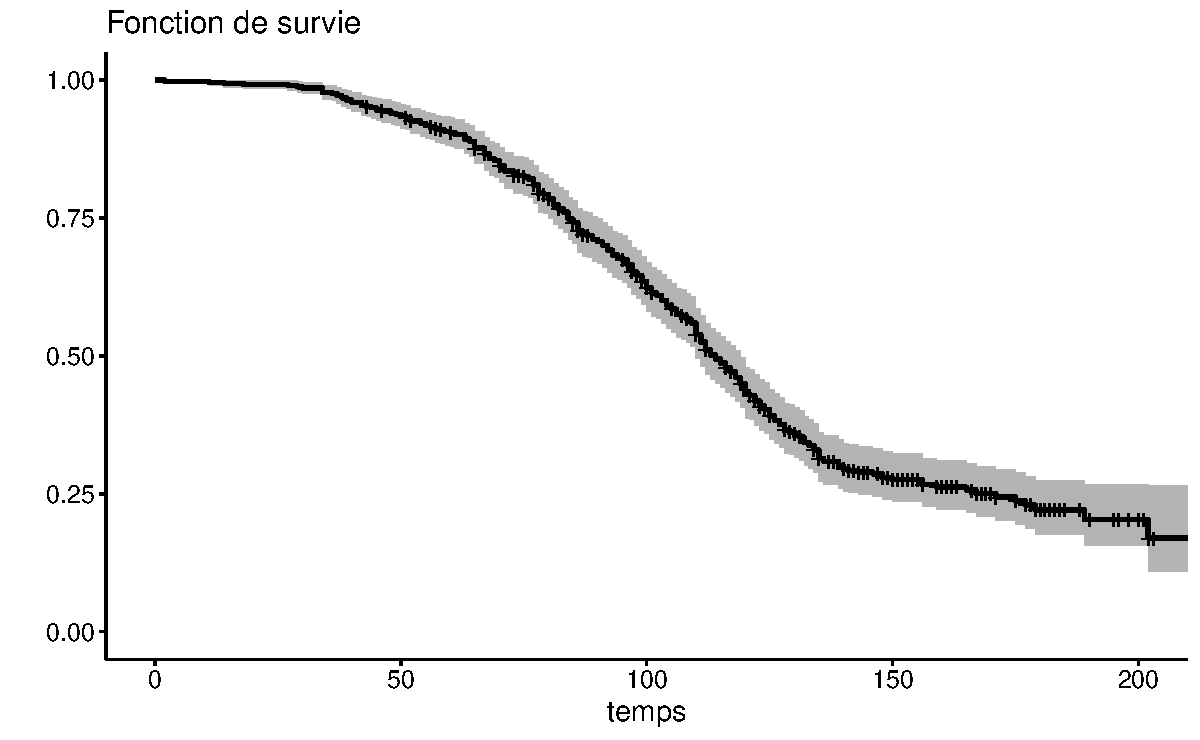
\includegraphics[width=0.9\textwidth,height=\textheight]{survie_files/figure-pdf/fig-km-survie1-1.pdf}

}

\caption{\label{fig-km-survie1}Estimation de Kaplan--Meier de la
fonction de survie pour les données d'abonnement avec intervalles de
confiance ponctuels à 95\%.}

\end{figure}%

On peut également utiliser la fonction \texttt{quantile} pour obtenir
une estimation des quartiles et un intervalle de confiance On utilise
généralement le temps de survie médian (au lieu de la moyenne) dans ce
type d'étude. Ici, l'estimé du temps de survie médian est de 114
semaines: on estime que la moitié des clients vont avoir une durée
d'abonnement supérieure à 114 semaines. De même, la moitié des clients
vont avoir une durée d'abonnement inférieure à 114 semaines. Un
intervalle de confiance de niveau 95\% pour ce temps médian est
{[}\(110; 119\){]}.

Un estimé de la moyenne et de l'écart-type est donné, mais ce dernier
est biaisé (trop bas) puisque les données censurées ne donnent qu'une
borne inférieure pour la vraie valeur. Avec un modèle paramétrique pour
la survie (par ex., une loi exponentielle), les paramètres estimés du
modèle dicteraient ces deux valeurs. Le modèle de Kaplan--Meier estime
la survie, mais si la plus grande observation est censurée, la courbe
n'atteindra pas zéro.

Le graphique de la fonction de survie permet de lire le temps de survie
pour une probabilité donnée. Les bandes donnent un intervalle de
confiance ponctuel de niveau 95\% pour chaque temps donné.

Une information pertinente de la sortie est le nombre de données
censurées: parmi les 500 observations, il y a 334 clients qui ont
terminé leur abonnement et 166 qui sont censurées (le client est
toujours abonné et le temps est donc une borne inférieure de la durée
d'abonnement). Les données censurées contiennent moins d'information que
les temps observés de défaillance puisqu'on sait uniquement la borne
inférieure de la plage possible des valeurs pour le vrai temps de
défaillance.

Les statistiques descriptives usuelles sont biaisées en raison de la
censure. Avec l'estimateur de Kaplan--Meier, on peut aisément obtenir
les quantiles. Si la courbe de survie estimée descend à zéro, il est
également possible d'estimer la moyenne en calculant l'aire sous la
courbe de survie.\footnote{Si on considère une variable aléatoire
  positive, alors l'aire sous la courbe de survie donne l'espérance.} Si
la courbe ne descend pas à zéro, on obtient une borne inférieure
(sous-estimation de la moyenne), appelée \emph{moyenne restreinte}.

\begin{Shaded}
\begin{Highlighting}[]
\FunctionTok{print}\NormalTok{(kapm, }\AttributeTok{print.rmean =} \ConstantTok{TRUE}\NormalTok{)}
\end{Highlighting}
\end{Shaded}

Par exemple, la moyenne estimée via Kaplan--Meier est 125 semaines
(\texttt{rmean}), à comparer avec la moyenne empirique de
\texttt{temps}, ici de 107.788 semaines, qui est biaisée.

\subsection{Calcul de l'estimateur de
Kaplan--Meier}\label{calcul-de-lestimateur-de-kaplanmeier}

Pour comprendre l'estimateur de Kaplan--Meier, il est utile de
s'intéresser à sa construction. Deux éléments sont essentiels: on parle
d'\textbf{échec} ou d'événement au temps \(t_i\) si l'événement est
observé (\(T_i=t_i\)) au temps \(t_i\). Le nombre de \textbf{personnes à
risque} au temps \(t_i\) est le total des observations dont le temps
mesuré excède \(t_i\) (censure et événements postérieurs à \(t_i\))

Pour la \textbf{construction}, on procède comme suit:

\begin{itemize}
\tightlist
\item
  Ordonner les temps (uniques) où il y a des échecs (temps où
  \texttt{censure\ =\ 1}), disons \(t_{(1)} \leq \cdots \leq t_{(m)}\)
\item
  À chaque temps \(t_{(i)}\) \((i=1, \ldots m)\), on calcule le nombre
  de personnes à risque, \(r_i\), et le nombre d'échecs, \(d_i\).
\item
  Le risque empirique est \(\widehat{h}_i = r_i/d_i\), la proportion
  d'échecs parmi les personnes à risque.
\end{itemize}

L'estimateur de Kaplan--Meier définit une \textbf{fonction escalier}

\begin{itemize}
\tightlist
\item
  Entre \(t=0\) et \(t=t_{(1)}\), la survie est de 1.
\item
  Entre \(t=t_{(1)}\) et \(t=t_{(2)}\), la survie est
  \(1-\widehat{h}_1\).
\item
  Entre \(t=t_{(2)}\) et \(t=t_{(3)}\), la survie est
  \((1-\widehat{h}_1) \times (1-\widehat{h}_2)\), etc.
\end{itemize}

Pour un temps \(t\) donné, on multiplie tous les termes
(\(1-\widehat{h}_i\)) des temps d'échecs passés, \begin{align*}
 \widehat{S}(t) &= \prod_{i: t_{(i)} < t} \left( 1- \widehat{h}_i\right) \\ &= \left( 1- \frac{d_1}{r_1}\right) \times \cdots \times \left( 1- \frac{d_{i(t)}}{r_{i(t)}}\right).
\end{align*} où \(i(t) =\max(j \in \{1, \ldots, m\}:  t \geq t_{j})\),
soit le plus grand indice parmi \(1, \ldots, m\) tel que
\(t \geq t_{i(t)}\). Par convention, si \(t < t_{(1)}\), on fixe
\(\widehat{S}(t)=1\). La fonction de survie n'est pas définie aux temps
de défaillance observée, mais la convention veut qu'elle soit continue à
gauche.

Ainsi, l'estimation de la survie estimée ne change qu'aux valeurs de
\(t_{(i)}\) (\(i=1, \ldots, m\)). Les contre-marches de l'escalier ainsi
défini interviennent uniquement aux temps observés d'échecs. Si à un
moment donné toutes les personnes à risque expérimentent l'événement, la
courbe descend à zéro. Si on a uniquement de la censure à droite, la
courbe de survie n'atteindra jamais zéro si la plus grande observation
est censurée à droite. Avec la troncation à gauche, la même logique
s'applique mais les personnes ne sont à risque qu'à partir du temps
minimum observé.

\section{Comparaison de deux courbes de
survie}\label{comparaison-de-deux-courbes-de-survie}

Supposons que les individus ont été divisés en deux groupes et que
\(S_1(t)\) et \(S_2(t)\) dénotent respectivement la fonction de survie
du premier groupe et du deuxième groupe. On est souvent intéressé à
tester l'égalité des fonctions de survie, c'est-à-dire, les hypothèses
\(\mathscr{H}_0: S_1(t) = S_2(t)\) pour tout \(t\) et
\(\mathscr{H}_1: S_1(t) \neq S_2(t)\) pour au moins une valeur de \(t\).

Par exemple, dans une étude sur le temps de survie après avoir été
diagnostiqué avec un certain type de cancer, on pourrait vouloir
comparer le temps de survie des individus ayant reçu le traitement
standard (groupe 1) au temps de survie des individus ayant reçu un
nouveau traitement (groupe 2).

Les deux tests utilisés habituellement sont le test du log-rang
(\emph{log-rank test}) et le test de Wilcoxon généralisé (ou test de
Gehan).

Testons l'hypothèse que la courbe de survie des clients masculins est la
même que celle des clients féminins dans l'exemple des données
d'abonnement:

\begin{Shaded}
\begin{Highlighting}[]
\NormalTok{strat\_sexe }\OtherTok{\textless{}{-}} \FunctionTok{survfit}\NormalTok{(}\FunctionTok{Surv}\NormalTok{(temps, censure) }\SpecialCharTok{\textasciitilde{}}\NormalTok{ sexe, }\AttributeTok{data =}\NormalTok{ survie1)}
\NormalTok{lograng }\OtherTok{\textless{}{-}} \FunctionTok{survdiff}\NormalTok{(}\FunctionTok{Surv}\NormalTok{(temps, censure) }\SpecialCharTok{\textasciitilde{}}\NormalTok{ sexe, }\AttributeTok{data =}\NormalTok{ survie1)}
\end{Highlighting}
\end{Shaded}

Si on utilise les méthodes (\texttt{print}, \texttt{summary},
\texttt{plot}, \texttt{quantile}) pour la sortie de \texttt{survfit}, on
obtiendra les résultats pour chaque strate (ou niveaux de la variable
catégorielle). Par exemple, il y a 309 hommes et 191 femmes et
l'estimation du temps de survie médian est de 110 semaines pour les
hommes et de 123 semaines pour les femmes.

La fonction \texttt{survdiff} avec la formule retourne le résultat du
test asymptotique du log-rang pour l'hypothèse d'égalité des fonctions
de survie. La statistique du khi-deux vaut 16.43 et la valeur-\(p\) du
test est inférieure à \(10^{-4}\): on rejette donc \(\mathscr{H}_0\)
pour conclure qu'il y a donc une différence significative entre les deux
courbes de survie.

Les courbes de survie selon le sexe sont représentées dans la
Figure~\ref{fig-survie-comparaison-courbes}. On voit que la courbe des
femmes est systématiquement au-dessus de celle des hommes. Les femmes
ont donc tendance à rester abonnées plus longtemps que les hommes, et
cette différence est significative.

\begin{Shaded}
\begin{Highlighting}[]
\FunctionTok{plot}\NormalTok{(}\FunctionTok{survfit}\NormalTok{(}\FunctionTok{Surv}\NormalTok{(temps, censure) }\SpecialCharTok{\textasciitilde{}}\NormalTok{ sexe, }
             \AttributeTok{data =}\NormalTok{ survie1), }
     \AttributeTok{conf.int =} \ConstantTok{FALSE}\NormalTok{,}
     \AttributeTok{col =} \FunctionTok{c}\NormalTok{(}\StringTok{"red"}\NormalTok{, }\StringTok{"blue"}\NormalTok{), }
     \AttributeTok{xlab =} \StringTok{"temps"}\NormalTok{, }
     \AttributeTok{ylab =} \StringTok{"fonction de survie"}\NormalTok{)}
\end{Highlighting}
\end{Shaded}

\begin{figure}[ht!]

\centering{

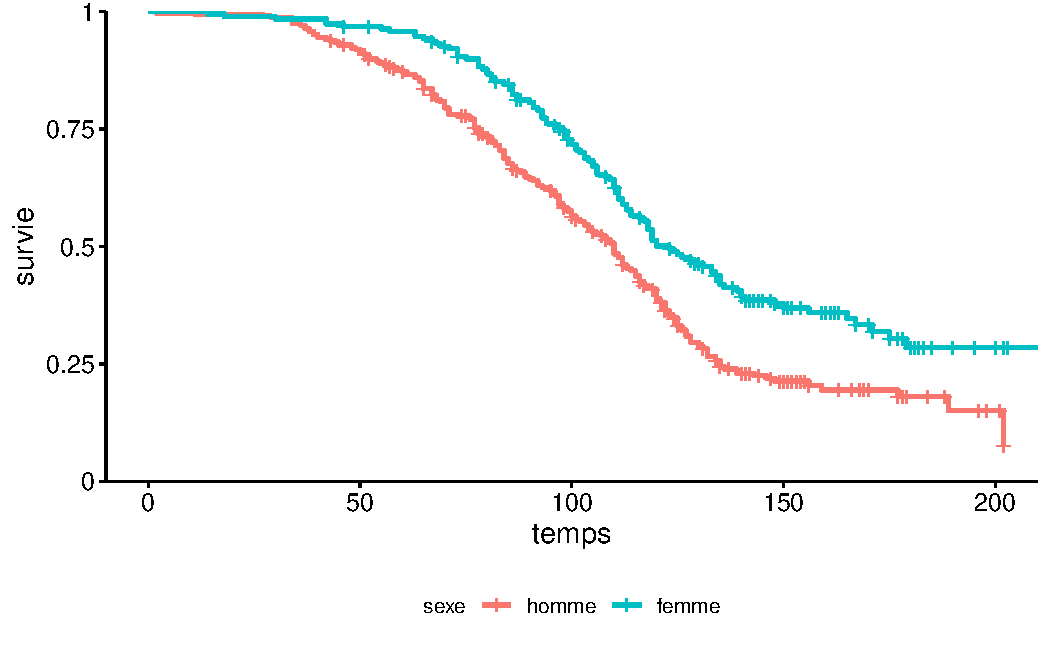
\includegraphics[width=0.9\textwidth,height=\textheight]{survie_files/figure-pdf/fig-survie-comparaison-courbes-1.pdf}

}

\caption{\label{fig-survie-comparaison-courbes}Courbes de survie pour
les durées d'abonnement selon le sexe de l'individu.}

\end{figure}%

Il est également possible de tester l'égalité des courbes de survie avec
plus de deux groupes. Par exemple, s'il y a \(k\) groupes, l'hypothèse
nulle est alors \(\mathscr{H}_0: S_1(t)=S_2(t)=\cdots = S_k(t)\) pour
tout \(t\), versus l'alternative qu'au moins deux des fonctions ont une
valeur différente pour au moins une valeur de \(t\); la loi nulle
asymptotique du test est alors \(\chi^2_{k-1}\).

L'estimateur de Kaplan--Meier ne permet pas l'inclusion de variables
explicatives à proprement parler: si on peut veut les différences au
niveau de la survie selon les modalités d'une variable explicative
catégorielle, on divise pour ce faire l'échantillon en sous-groupes et
on utilise l'estimateur de Kaplan--Meier pour chacune des modalités en
gardant en tête que cela réduit la taille de l'échantillon disponible et
que l'estimation résultante est possiblement trop incertaine pour être
utile.

\begin{tcolorbox}[enhanced jigsaw, bottomrule=.15mm, toptitle=1mm, opacityback=0, title=\textcolor{quarto-callout-note-color}{\faInfo}\hspace{0.5em}{En résumé}, left=2mm, bottomtitle=1mm, colbacktitle=quarto-callout-note-color!10!white, colback=white, breakable, toprule=.15mm, coltitle=black, arc=.35mm, opacitybacktitle=0.6, colframe=quarto-callout-note-color-frame, titlerule=0mm, leftrule=.75mm, rightrule=.15mm]

\begin{itemize}
\tightlist
\item
  L'analyse de survie est l'étude de temps d'attente (variable positive)
  avant que survienne un événement.
\item
  L'étude des temps de défaillance nécessite l'utilisation d'outils
  statistiques spécifiques en raison des mécanismes de censure et de
  troncation.
\item
  La fonction de survie \(S(t)\) encode la probabilité que le temps de
  défaillance excède le temps \(t\).
\item
  La fonction de risque encode la probabilité de mourir au temps \(t\)
  sachant qu'on a survécu jusque là.
\item
  La connaissance de la fonction de survie permet d'obtenir la fonction
  de risque et vice-versa.
\item
  Le mécanisme d'information partielle le plus courant en analyse de
  survie est la censure à droite (on ne connaît qu'une borne inférieure
  pour le temps de défaillance, l'événement n'étant toujours pas survenu
  au temps donné).
\item
  Si on traitait les temps de censure comme des temps de défaillance
  observée, on \emph{sous-estimerait} la durée de survie.
\item
  L'estimateur de Kaplan--Meier est l'estimateur du maximum de
  vraisemblance nonparamétrique si on a de la censure à droite aléatoire
  ou non-informative. Il ne fait aucun postulat sur la distribution de
  la survie.
\item
  Pour que l'estimation soit de qualité, il faut un nombre
  \emph{conséquent} d'observations (disons 1000). La quantité
  d'observations censurées impacte la précision de l'estimation.
\item
  L'estimateur est déficient si le plus grand temps observé est censuré
  à droite (l'estimation de la fonction de survie ne décroît pas à
  zéro).
\item
  Le test du log-rang permet de valider si deux fonctions de survie sont
  égales (en tout temps).
\item
  On peut estimer la fonction de survie indépendamment pour chaque
  modalité d'une variable explicative catégorielle en stratifiant: cela
  réduit la taille de l'échantillon pour chaque strate.
\item
  Le modèle de Kaplan--Meier ne permet pas d'estimer l'impact de
  variables explicatives sur la survie.
\end{itemize}

\end{tcolorbox}

\section{Modèle à risques proportionnels de
Cox}\label{moduxe8le-uxe0-risques-proportionnels-de-cox}

Le modèle à risques proportionnels de Cox (\emph{proportional hazard
model}) est l'un des modèles les plus utilisés pour l'analyse des
données de survie.

\subsection{Description du modèle de
Cox}\label{description-du-moduxe8le-de-cox}

Soit \(h(t; \boldsymbol{x})\) la valeur de la fonction de risque au
temps pour un individu dont les valeurs des variables explicatives sont
\(X_1=x_1, \ldots, X_p=x_p\). Le modèle à risques proportionnels est
\begin{align*}
h(t; \boldsymbol{x}) = h_0(t)\exp(\beta_1x_1 + \cdots + \beta_p x_p)
\end{align*} où \(h_0(t)\) est la fonction de risque de base; il n'est
pas nécessaire de spécifier cette dernière, d'où la nature
semiparamétrique du modèle de Cox. Le postulat de risques proportionnels
implique que le terme de droite \(\exp(\mathbf{X}\boldsymbol{\beta})\)
ne dépend pas du temps, et plus particulièrement
\(\beta_1, \ldots, \beta_p\) ne varie pas en fonction de \(t\). Nous
verrons subséquemment une extension pour accomoder ce cas de figure.

Lorsque toutes les variables explicatives prennent la valeur zéro,
\(\boldsymbol{X}=\boldsymbol{0}\), on recouvre
\(h(t; \boldsymbol{0})= h_0(t)\). Par conséquent, la fonction \(h_0(t)\)
peut être interprétée comme la fonction de risque lorsque toutes les
variables explicatives valent zéro. Toutefois, tout comme la valeur de
l'ordonnée à l'origine dans un modèle de régression linéaire, cette
interprétation n'est pas nécessairement valide si la situation où toutes
les variables explicatives valent zéro n'est pas possible ou si elle ne
survient pas dans notre échantillon.

La deuxième partie du modèle,
\(\exp(\beta_1x_1 + \cdots + \beta_p x_p)\), vient modéliser l'effet
d'un changement des valeurs des variables explicatives sur la fonction
de risque de base. Tout comme dans le cas de la régression logistique
(l'effet des variables sur la cote), c'est un effet multiplicatif, d'où
le terme \textbf{risques proportionnels}.

Pour l'interprétation des paramètres, il sera plus simple de penser en
termes de rapport de risque (\emph{hazard ratio}), qui est défini comme
étant le rapport des fonctions de risque pour deux ensembles de valeurs
des variables explicatives. Pour simplifier l'illustration, supposons
que nous avons seulement une variable explicative \(X\) et que
\(h(t; x) = h_0(t)\exp(\beta x)\). Le rapport de risque lorsque
\(X=x_1\) par rapport à \(X=x_0\) est \begin{align*}
\frac{h(t; x_1)}{h(t; x_0)} = \exp\{\beta(x_1-x_0)\}.
\end{align*} Par conséquent, l'impact d'une augmentation de \(X\) d'une
unité (quand \(x_1-x_0=1\)) est \(\exp(\beta)\). Ainsi, pour chaque
augmentation d'une unité pour \(X\), le risque que l'événement survienne
est multiplié par \(\exp(\beta)\).

Le terme \textbf{risques proportionnels} fait référence à la situation
où le rapport de risque dépend seulement de la différence \(x_1-x_0\) et
non pas du temps lui-même. Le rapport de risque est constant par rapport
au temps \(t\). Cela implique que l'effet d'une variable est stable dans
le temps. Nous verrons plus loin comment faire en sorte que l'effet
d'une variable puisse varier dans le temps.

Débutons avec un exemple simple en utilisant les données d'abonnement:
on ajuste un modèle de Cox en utilisant seulement la variable binaire
sexe.

\begin{Shaded}
\begin{Highlighting}[]
\NormalTok{cox1 }\OtherTok{\textless{}{-}} \FunctionTok{coxph}\NormalTok{(}\FunctionTok{Surv}\NormalTok{(temps, censure) }\SpecialCharTok{\textasciitilde{}}\NormalTok{ sexe, }
              \AttributeTok{data =}\NormalTok{ survie1,}
              \AttributeTok{ties =} \StringTok{"exact"}\NormalTok{)}
\CommentTok{\# Coefficients, tests et IC 95\% de Wald}
\FunctionTok{summary}\NormalTok{(cox1)}
\CommentTok{\# Test du rapport de vraisemblance}
\NormalTok{car}\SpecialCharTok{::}\FunctionTok{Anova}\NormalTok{(cox1, }\AttributeTok{type =} \DecValTok{3}\NormalTok{)}
\end{Highlighting}
\end{Shaded}

La sortie inclut notamment des tests de significativité globale basés
sur la vraisemblance comparant le modèle sans variable explicative avec
celui ajusté (rapport de vraisemblance, score et Wald). Ces trois
statistiques ciblent la même hypothèse, aussi on peut ne s'attarder
qu'au test du rapport de vraisemblance, qui est plus fiable et
généralement plus puissant. Le tableau des coefficients donne les
estimations \(\widehat{\beta}\). Le rapport de risque pour
\texttt{sexe=1} versus \texttt{sexe=0} est \(\exp(\widehat{\beta})\),
tandis qu'on obtiendrait le rapport de risque pour \texttt{sexe=0}
versus \texttt{sexe=1}, soit \(\exp(-\widehat{\beta})\). Les
statistiques de test et la valeur-\(p\) associée sont basées sur la
statistique de Wald, soit
\(\widehat{\beta}/\mathsf{se}(\widehat{\beta})\), tandis que les
intervalles de confiance à 95\% pour le rapport de risque sont des
intervalles de Wald de la forme
\(\exp\{\widehat{\beta} \pm 1.96 \cdot \mathsf{se}(\widehat{\beta})\}\)
pour le rapport de risque. Un rapport de risque de 1 signifie que le
risque n'est pas affecté par la variable explicative. Ici, le test
correspondant à l'hypothèse nulle \(\beta=0\) ne mène pas au rejet de
l'hypothèse qui veut que la variable n'impacte pas le risque. On
pourrait obtenir les intervalle

\begin{longtable}[t]{lrrr}

\caption{\label{tbl-cox1}Rapport de risques et intervalles de confiance
de Wald à niveau 95\%.}

\tabularnewline

\toprule
terme & exp(coef) & borne inf. & borne sup.\\
\midrule
sexe & 0.63 & 0.5 & 0.79\\
\bottomrule

\end{longtable}

Il y a une seule variable explicative, le sexe de l'individu.
L'estimation du paramètre de l'effet de sexe est -0.47. Ce paramètre est
significativement différent de \(0\) (valeur-\(p\) du test du rapport de
vraisemblance inférieure à \(10^{-10}\)). Pour l'interprétation, on
utilise la colonne \texttt{exp(coef)} qui contient la valeur
\(\exp(\hat{\beta}_{\texttt{sexe}}) = \exp(-0.466) = 0.628\). Ainsi, le
rapport du risque d'une femme par rapport à un homme est \begin{align*}
 \frac{\hat{h}(t; \texttt{sexe}=1)}{\hat{h}(t; \texttt{sexe}=0)}= 0.628.
\end{align*} Par conséquent, le risque qu'une femme interrompe son
abonnement est 0.628 fois celui d'un homme. Une femme est donc moins à
risque de quitter qu'un homme. Nous avions déjà vu cela à la section
précédente lorsque nous avions comparé les courbes de survie des hommes
et des femmes. Il est important de se rappeler qu'avec ce modèle,
l'effet d'une variable est le même dans le temps (peu importe la valeur
de \(t\)). Donc, une femme est moins à risque de quitter qu'un homme à
tout moment, d'après ce modèle. Inversement, le ratio du risque d'un
homme par rapport à une femme est
\(\exp(-\hat{\beta}_{\texttt{sexe}}) = 1/0.628=1.59\). Ainsi, à tout
moment, un homme a un risque d'interrompre son abonnement qui est 59\%
plus élevé que celui d'une femme.

Comme il y a un seul paramètre ici, les tests basés sur la vraisemblance
pour \(\mathscr{H}_0: \boldsymbol{\beta}=\boldsymbol{0}\) reviennent à
tester l'effet de la variable sexe. Le test de Wald est le même que
celui du tableau des coefficients. Dans le cas particulier où il y a une
seule variable explicative catégorielle comme ici, le test du score est
équivalent au test du log-rang que nous avons vu à la section précédente
à une petite différence près lorsqu'il y a des doublons (ex aequo) dans
les temps de survie.

On pourrait également utiliser une variable explicative continue plutôt
qu'une variable binaire; le principe est le même.

\begin{Shaded}
\begin{Highlighting}[]
\NormalTok{cox2 }\OtherTok{\textless{}{-}} \FunctionTok{coxph}\NormalTok{(}\FunctionTok{Surv}\NormalTok{(temps, censure) }\SpecialCharTok{\textasciitilde{}}\NormalTok{ age, }
              \AttributeTok{data =}\NormalTok{ survie1,}
              \AttributeTok{ties =} \StringTok{"exact"}\NormalTok{)}
\FunctionTok{summary}\NormalTok{(cox2)}
\end{Highlighting}
\end{Shaded}

Le rapport de risque pour âge est 0.959 et donc le risque diminue de
4.1\% chaque fois que l'âge augmente d'un an --- le risque d'interrompre
l'abonnement diminue lorsque l'âge augmente et cet effet est
significatif (valeur-\(p\) du test de significativité globale
inférieures à \(10^{-4}\)).

Généralement, on considérera le modèle de Cox avec toutes les variables
explicatives simultanément. La variable \(\texttt{region}\) est nominale
tandis que la variable \(\texttt{service}\) est ordinale (avec quatre
modalités). Nous allons les incorporer, comme d'habitude, en utilisant
des variables indicatrices avec \(\texttt{region=1}\) et
\(\texttt{service=0}\) (le client n'est abonné à aucun autre service)
comme catégories de référence.

\begin{Shaded}
\begin{Highlighting}[]
\FunctionTok{with}\NormalTok{(survie1, }\FunctionTok{table}\NormalTok{(service))}
\NormalTok{cox3 }\OtherTok{\textless{}{-}} \FunctionTok{coxph}\NormalTok{(}\FunctionTok{Surv}\NormalTok{(temps, censure) }\SpecialCharTok{\textasciitilde{}} 
\NormalTok{                age }\SpecialCharTok{+}\NormalTok{ sexe }\SpecialCharTok{+}\NormalTok{ region }\SpecialCharTok{+}\NormalTok{ service, }
              \AttributeTok{data =}\NormalTok{ survie1, }
              \AttributeTok{ties =} \StringTok{"exact"}\NormalTok{)}
\FunctionTok{summary}\NormalTok{(cox3)}
\CommentTok{\# Effets de type 3 }
\CommentTok{\# (modèle avec toutes les variables sauf une)}
\NormalTok{car}\SpecialCharTok{::}\FunctionTok{Anova}\NormalTok{(cox3, }
           \AttributeTok{type =} \DecValTok{3}\NormalTok{)}
\end{Highlighting}
\end{Shaded}

\begin{longtable}[t]{lrrr}

\caption{\label{tbl-survie5-coefs}Rapport de risque et intervalles de
confiance à niveau 95\% de Wald pour le modèle de Cox de base avec
toutes les variables explicatives.}

\tabularnewline

\toprule
terme & exp(coef) & borne inf. & borne sup.\\
\midrule
age & 0.95 & 0.94 & 0.96\\
sexe & 0.51 & 0.40 & 0.65\\
region2 & 0.67 & 0.47 & 0.98\\
region3 & 1.03 & 0.73 & 1.46\\
region4 & 0.80 & 0.57 & 1.13\\
\addlinespace
region5 & 0.97 & 0.68 & 1.37\\
service1 & 0.35 & 0.27 & 0.45\\
service2 & 0.17 & 0.12 & 0.25\\
service3 & 0.12 & 0.07 & 0.19\\
\bottomrule

\end{longtable}

\begin{longtable}[t]{lrrl}

\caption{\label{tbl-survie5-deviance}Tests du rapport de vraisemblance
pour les effets de type III pour le modèle de Cox avec toutes les
variables explicatives.}

\tabularnewline

\toprule
terme & statistique & ddl & valeur-p\\
\midrule
age & 68.07 & 1 & <0.0001\\
sexe & 32.82 & 1 & <0.0001\\
region & 7.67 & 4 & 0.1\\
service & 159.31 & 3 & <0.0001\\
\bottomrule

\end{longtable}

Les effets des variables sont maintenant des effets marginaux. Ainsi,
lorsque les autres variables demeurent fixes, le risque de quitter d'une
femme est 0.511 fois plus petit que celui d'un homme. L'effet marginal
(une fois que les autres variables sont incluses) de la variable sexe
est significatif (valeur-\(p\) inférieure à \(10^{-4}\)).

Toutes autres choses étant égales, chaque augmentation de l'âge d'un an
fait diminuer le risque d'interrompre l'abonnement. Plus précisément, le
risque est multiplié par 0.95 lorsque l'âge augmente d'un an et cet
effet est significatif.

Pour la variable service, l'interprétation se fait par rapport à la
catégorie de référence, qui est la catégorie \(\texttt{0}\) (abonné à
aucun autre service). Ainsi, si le client est abonné à un autre service,
son risque de quitter est 0.353 fois celui d'un client qui n'est pas
abonné à un autre service (toutes autres choses étant égales). Si le
client est abonné à deux autres services, son risque de quitter est
encore plus petit comparativement à un client qui n'est pas abonné à un
autre service (rapport de risque de 0.174) Finalement, si le client est
abonné à trois autres services, son risque de quiter est encore plus
petit (rapport de risque de 0.115). Les paramètres de ces trois
variables sont tous significatifs. Ainsi, les clients qui sont abonnés à
un, deux ou trois services ont un risque de quitter qui est
significativement plus faible que celui d'un client qui n'est pas abonné
à un autre service. Le tableau d'analyse de déviance (effets de type 3)
donne les statistiques du rapport de vraisemblance pour tester
globalement la significativité d'une variable explicative modélisée avec
plusieurs indicatrices. Pour la variable \(\texttt{service}\), le test
présenté teste l'hypothèse nulle
\(\mathscr{H}_0: \beta_{\texttt{service}_1}=\beta_{\texttt{service}_2}=\beta_{\texttt{service}_3}=0\)
contre l'alternative qu'un moins un de ces trois paramètres est non-nul.
Le test est largement significatif (statistique du rapport de
vraisemblance valant 159.31 avec une valeur-\(p\) inférieure à
\(10^{-4}\)). L'effet de la variable \(\texttt{service}\) est donc
globalement significatif. Afin de comparer les autres modalités entre
elles, par exemple afin de voir si le risque de quitter est différent
entre un client qui a deux services et un autre qui a trois services, il
suffit de changer la catégorie de référence à la commande \texttt{class}
et de réajuster le modèle.

Finalement, la variable \(\texttt{region}\) n'est pas globalement
significative (statistique du rapport de vraisemblance de 7.67 avec une
valeur-\(p\) de 0.1 basée sur la loi asymptotique \(\chi^2_4\)).

\subsection{Estimation de la fonction de survie pour des valeurs
particulières des variables
explicatives}\label{estimation-de-la-fonction-de-survie-pour-des-valeurs-particuliuxe8res-des-variables-explicatives}

Il est possible d'obtenir l'estimation de la fonction de survie pour des
valeurs particulières des variables explicatives. Pour ce faire, il faut
avoir un autre fichier de données qui contient les valeurs des variables
explicatives pour lesquelles on veut une estimation de la fonction de
survie. Si on ajuste le modèle avec aucune variable explicative, on
retrouvera alors l'estimation de Kaplan--Meier de la fonction de survie.

Supposons qu'on ajuste le modèle avec les variables sexe et âge
seulement dans l'exemple du temps d'abonnement, et que l'on désire la
fonction de survie pour les hommes de 25 et 60 ans et pour les femmes de
25 et 60 ans. Le fichier \texttt{survie2} contient les données qui
seront utilisées à cette fin.

\begin{figure}[ht!]

\centering{

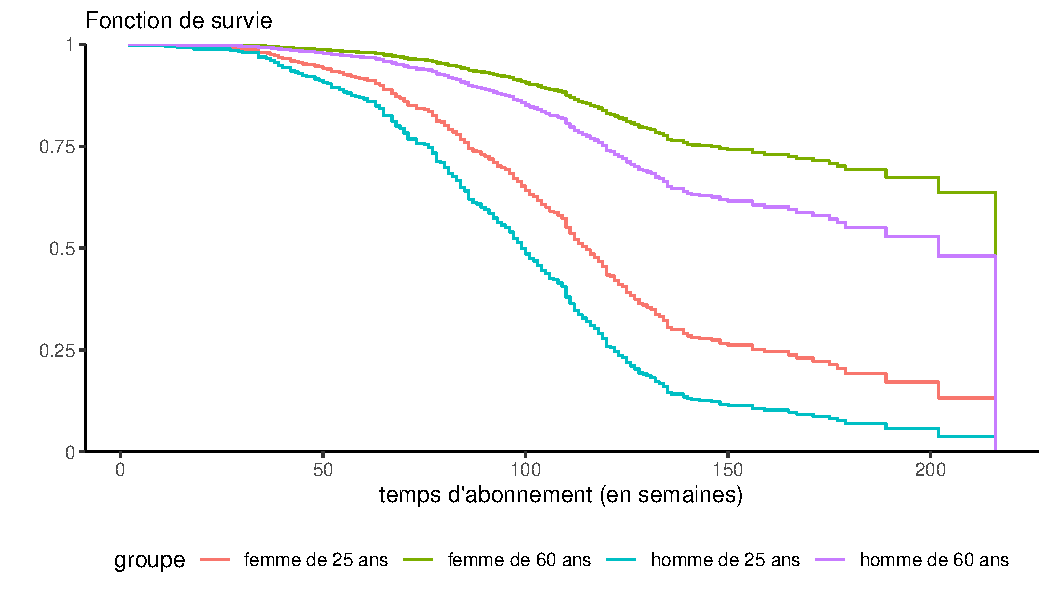
\includegraphics[width=0.8\textwidth,height=\textheight]{survie_files/figure-pdf/fig-courbes-survie-1.pdf}

}

\caption{\label{fig-courbes-survie}Courbes de survies du modèle de Cox
pour les quatre profils client.}

\end{figure}%

Les quatre fonctions de la Figure~\ref{fig-courbes-survie} correspondent
aux profils pour lesquels nous désirons une estimation de la courbe de
survie. La courbe 1 est pour les hommes de 25 ans, la courbe 2 pour les
femmes de 25 ans, la courbe 3 pour les hommes de 60 ans et la courbe 4
pour les femmes de 60 ans. On voit donc que, parmi ces quatre profils,
les hommes de 25 ans sont le plus à risque de quitter tandis que les
femmes de 60 ans sont le moins à risque de quitter.

\subsection{Variables explicatives dont la valeur change dans le
temps}\label{variables-explicatives-dont-la-valeur-change-dans-le-temps}

Il est clair que certaines caractéristiques d'un individu évoluent dans
le temps (\emph{time-varying covariates}). Si le sexe d'un individu est
stable dans le temps, son revenu, son statut matrimonial, l'endroit où
il habite, sont par contre des caractéristiques qui peuvent changer dans
le temps. Il peut alors être intéressant d'en tenir compte dans
l'analyse. Rappelez-vous que le modèle à risques proportionnels est
\begin{align*}
h(t; \boldsymbol{x}) = h_0(t) \exp(\beta_1x_1 + \cdots + \beta_px_p).
\end{align*}

Supposons que la variable \(X_1\) change au fil du temps et que les
autres demeurent fixes. On peut alors réécrire le modèle \begin{align*}
h(t; \boldsymbol{x}) = h_0(t) \exp\{\beta_1x_1(t) + \cdots + \beta_px_p\},
\end{align*} où \(x_1(t)\) indique que la valeur de \(X_1\) dépend du
temps \(t\).

Supposons que la variable \(\texttt{service}\), qui représente le nombre
d'autres services souscrits, est la seule que nous voulons modéliser
comme une variable qui varie dans le temps. Pour l'âge, nous prenons
simplement l'âge au début de l'abonnement, idem pour la région.

Le plus difficile est de créer correctement le fichier de données pour
effectuer ce genre d'analyse. Pour chaque personne, on peut identifier
plusieurs moments où l'une ou l'autres des valeurs des variables
explicatives change. Supposons qu'on a observé un événement au temps
\(t_1\), et que la valeur de la covariable change à \(t_0\), où
\(0 < t_0 < t_1\). On peut envisager cette observation donne deux
contributions: une pour la trajectoire sur l'intervalle \((0, t_0]\)
(censure à droite) et l'autre, après la modification, sur l'intervalle
\((t_0, t_1]\) (troncature à gauche). Puisque la valeur est observée
passée le premier intervalle, on a besoin de l'information sur toute la
fenêtre (les deux bornes) et le type d'événement pour la première
fenêtre sera de la censure à droite.

\begin{figure}[ht!]

\centering{

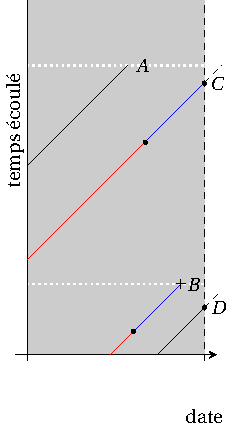
\includegraphics[width=0.35\textwidth,height=\textheight]{figures/Lexis_censure_modif.pdf}

}

\caption{\label{fig-lexischtemps}Diagramme de Lexis avec trajectoires.
Pour ajuster le modèle, on peut casser la contribution d'une observation
en segments: considérons un seul changement survenant au temps \(t_c\).
Pour le premier segment, on enregistre \(t_c\) comme valeur maximale
(censure à droite), tandis que pour la deuxième portion, l'observation
est tronquée à gauche à partir de \(t_c\).}

\end{figure}%

La base de données \texttt{survie3} contient le format adéquat: une
colonne \texttt{evenement} qui indique la censure (tout intervalle
intermédiaire pour un individu est traité comme de la censure à droite)
et les bornes de la fenêtre, \texttt{debut} et \texttt{fin}. Dans cet
exemple, il y a eu au plus un changement dans la variable
\(\texttt{service}\), comme présenté dans le fichier \texttt{survie3}.
Les variables explicatives \(\texttt{age}\), \(\texttt{sexe}\) et
\(\texttt{region}\) sont comme précédemment.

\begin{longtable}[t]{rrrrrrll}

\caption{\label{tbl-survie3-donnees}Aperçu des cinq premières
observations de la base de données \texttt{survie3}.}

\tabularnewline

\toprule
id & debut & fin & evenement & age & sexe & region & service\\
\midrule
1 & 0 & 130 & 0 & 48 & 1 & 3 & 2\\
1 & 130 & 178 & 0 & 48 & 1 & 3 & 1\\
2 & 0 & 159 & 0 & 31 & 1 & 3 & 2\\
3 & 0 & 110 & 1 & 36 & 1 & 4 & 0\\
4 & 0 & 109 & 1 & 30 & 0 & 2 & 0\\
\addlinespace
5 & 0 & 78 & 0 & 22 & 0 & 5 & 1\\
5 & 78 & 108 & 1 & 22 & 0 & 5 & 0\\
\bottomrule

\end{longtable}

On regarde plus en détail le profil des cinq premiers clients présenté
dans le Tableau~\ref{tbl-survie3-donnees}, dont seuls deux ont changé le
nombre d'abonnements; les individus 3--5 se sont désabonnés du service
cellulaire à un moment donné. Le premier client était abonné à deux
autres services au début de son abonnement au téléphone cellulaire mais,
après 130 semaines d'abonnement, a effectué un changement à son forfait
pour ne conserver qu'un autre service en plus du cellulaire. Pour le
deuxième client, comme \(\verb+temps_ch+\) est manquante, il est
toujours abonné à deux autres services et ce, jusqu'à la fin de l'étude.

\begin{Shaded}
\begin{Highlighting}[]
\FunctionTok{data}\NormalTok{(survie3, }\AttributeTok{package =} \StringTok{"hecmulti"}\NormalTok{)}
\NormalTok{cox4 }\OtherTok{\textless{}{-}} \FunctionTok{coxph}\NormalTok{(}\FunctionTok{Surv}\NormalTok{(}\AttributeTok{time =}\NormalTok{ debut, }
                   \AttributeTok{time2 =}\NormalTok{ fin, }
                   \AttributeTok{event =}\NormalTok{ evenement) }\SpecialCharTok{\textasciitilde{}} 
\NormalTok{                age }\SpecialCharTok{+}\NormalTok{ sexe }\SpecialCharTok{+}\NormalTok{ region }\SpecialCharTok{+}\NormalTok{ service, }
              \AttributeTok{data =}\NormalTok{ survie3)}
\end{Highlighting}
\end{Shaded}

L'interprétation se fait comme précédemment; on a omis l'option
\texttt{ties\ =\ "exact"} parce que cette option est trop gourmande en
calcul. Puisque c'est la valeur d'une variable qui varie dans le temps
et non pas son effet, on a l'interprétation usuelle. Par exemple, le
risque de quitter pour un client qui a un autre service est 0.601 fois
celui d'un client qui n'a aucun autre service (référence). Le fait
d'avoir deux ou trois services diminue encore plus le risque de quitter
(rapports de risque de 0.265 et 0.209, respectivement).

\subsection{Postulat de risques
proportionnels}\label{postulat-de-risques-proportionnels}

Le modèle de Cox fait l'hypothèse que la fonction de risque de base est
identique peut importe la valeur des variables catégorielles. La
Figure~\ref{fig-risquepropfig} illustre à quoi ce postulat correspond
dans un cas simple où il y a uniquement une variable binaire
explicative.

\begin{figure}[ht!]

\centering{

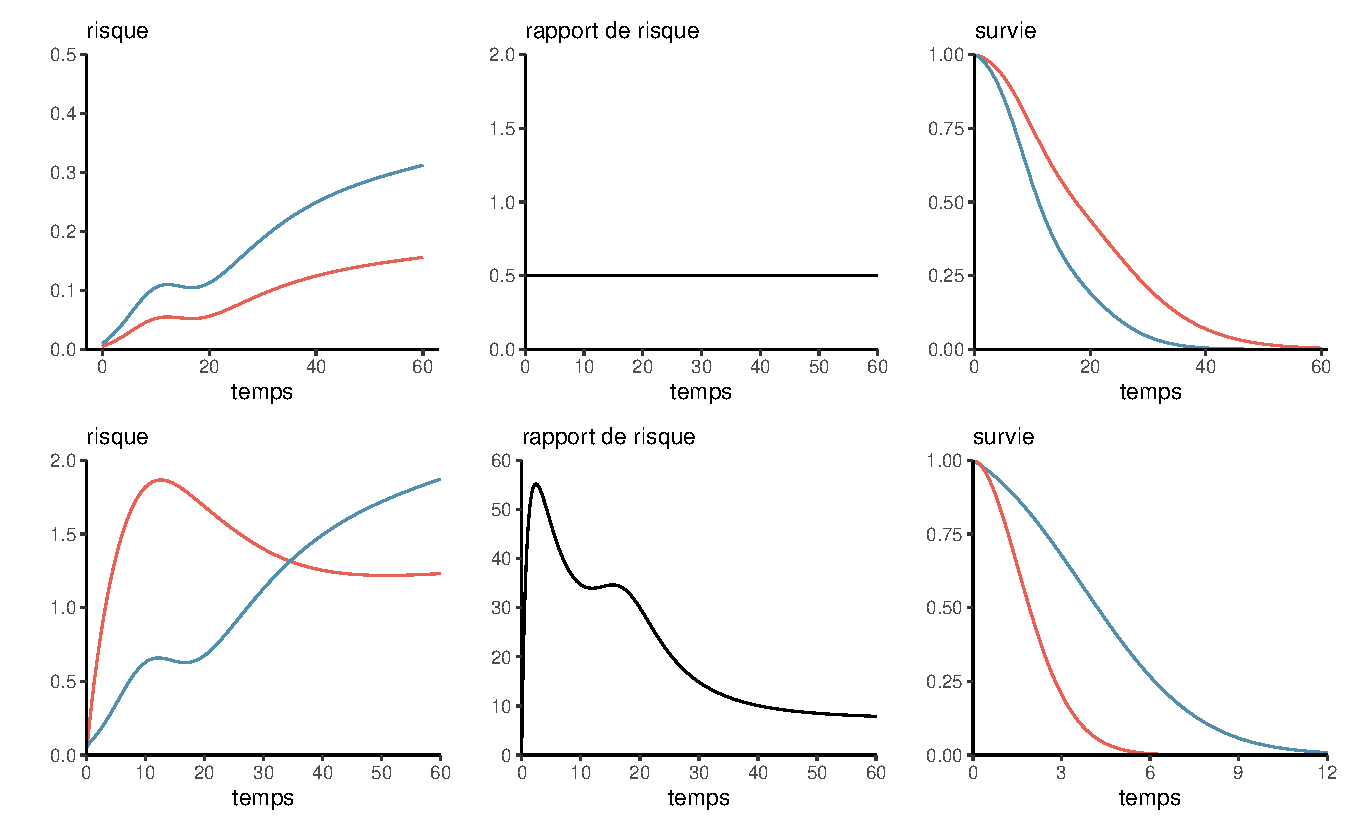
\includegraphics[width=0.9\textwidth,height=\textheight]{survie_files/figure-pdf/fig-risquepropfig-1.pdf}

}

\caption{\label{fig-risquepropfig}Courbes de risques proportionnelles
(panneau supérieur) et non proportionnelles (panneau inférieur) avec
rapport de risque et fonctions de survie correspondantes.}

\end{figure}%

Si ce n'est pas le cas, alors les résultats du modèle ne sont pas
nécessairement fiables.Comme pour un modèle de régression, il est
possible de créer des résidus du modèles et de faire des graphiques
diagnostics pour potentiellement infirmer le postulat de risques
proportionnels (\citeproc{ref-Grambsch.Therneau:1994}{Grambsch and
Therneau 1994}). Si l'hypothèse tient la route, alors il ne devrait pas
y avoir de tendance temporelle dans les résidus.

La commande \texttt{cox.zph} permet de tester le postulat de risques
proportionnels à l'aide d'un test du score pour voir si la pente
\(\beta(t)\) associée à une covariable est constante en fonction du
temps \(t\) pour tout temps; si la valeur-\(p\) est grande, cela indique
une absence de preuve contre l'hypothèse nulle \(\mathscr{H}_0\):
\(\{\beta(t)=c\) pour tout \(t\}\). La fonction \texttt{plot} permet
également d'obtenir un graphique des résidus en fonction du temps.

\begin{figure}[ht!]

\centering{

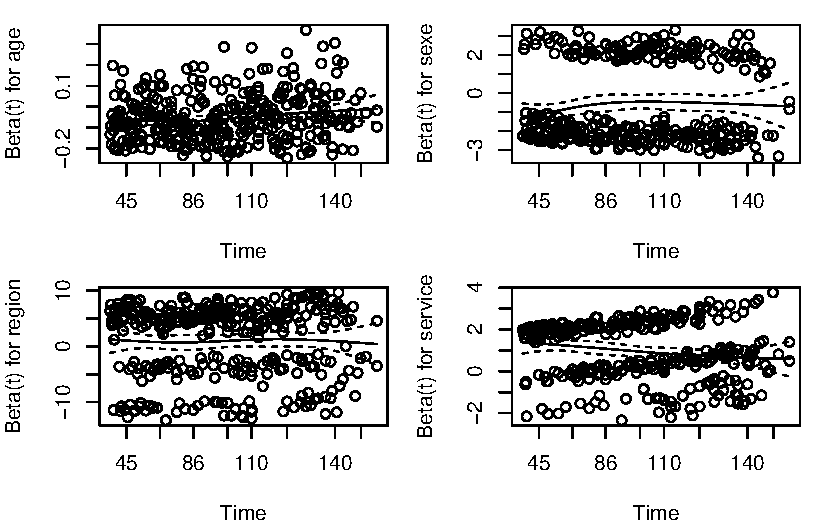
\includegraphics[width=0.85\textwidth,height=\textheight]{survie_files/figure-pdf/fig-coxphhypothese-1.pdf}

}

\caption{\label{fig-coxphhypothese}Estimations des coefficients en
fonction du temps basés sur les moindres carrés pondérés (diagnostic
graphique de Grampsch et Therneau).}

\end{figure}%

\begin{longtable}[t]{lrrl}

\caption{\label{tbl-coxphhypothese}Postulat de risques proportionnels:
test du score de Grampsch et Therneau (1994) pour les coefficients
constants dans le temps et valeur-p asymptotique basée sur la loi nulle
khi-deux.}

\tabularnewline

\toprule
effet & score & ddl & valeur-p\\
\midrule
age & 4.22 & 1 & 0.040\\
sexe & 1.11 & 1 & 0.291\\
region & 3.81 & 4 & 0.432\\
service & 10.97 & 3 & 0.012\\
global & 21.23 & 9 & 0.012\\
\bottomrule

\end{longtable}

Dans la Figure~\ref{fig-coxphhypothese}, on voit que le coefficient pour
service augmente au fil du temps pour tous les groupes. On pourrait
capturer cette interaction ou stratifier pour calculer le risque selon
le nombre de services, au risque d'avoir trop peu d'observations pour
estimer de manière fiable le risque de base. C'est explicable par le
fait que les personnes avec plus de services tendent à avoir une survie
plus longue.

\begin{Shaded}
\begin{Highlighting}[]
\NormalTok{diag\_risqueprop }\OtherTok{\textless{}{-}} \FunctionTok{cox.zph}\NormalTok{(cox3)}
\FunctionTok{print}\NormalTok{(diag\_risqueprop)}
\FunctionTok{plot}\NormalTok{(diag\_risqueprop)}
\end{Highlighting}
\end{Shaded}

Si le postulat n'est pas validé, on peut interpréter l'effet comme un
rapport de risque moyen pondéré sur la période de suivi, mais ce dernier
change selon le moment (\citeproc{ref-Stensrud.Hernan:2020}{Stensrud and
Hernán 2020}). Cela implique également que les erreurs-types associées
aux estimations sont trompeuses. La section suivante permettra de
généraliser le modèle de Cox et traiter ce cas de figure.

\subsection{Stratification}\label{stratification}

Une manière de modéliser la non-proportionnalité pour une variable
catégorielle est par la stratification. Supposons que nous avons une
variable explicative catégorielle \(Z=1, \ldots, K\) pour lequel le
postulat de risque proportionnels n'est pas valide. On s'intéresse à
l'effet des variables \(\mathbf{X}\). Typiquement, on ne s'intéresse pas
directement à l'effet de la variable \(Z\). Le modèle de Cox avec
stratification (pour la variable \(Z\)) est \begin{align*}
h(t; \mathbf{x}, z=k) = h_k(t) \exp(\boldsymbol{\beta} \mathbf{x}),
\end{align*} où \(h_k(t)\) est la fonction de risque de base quand
\(Z=k\) (\(k=1, \ldots, K\)). L'effet des autres variables explicatives
\(\mathbf{X}\) est supposé être le même peut importe la valeur de \(Z\),
mais la fonction de risque de base peut différer. Le rapport de risque
pour \(Z=k\) versus \(Z=j\) est \(h_k(t)/h_j(t)\); cette quantité dépend
du temps \(t\), mais pas des autres caractéristiques mesurées par
\(\mathbf{X}\). L'effet de la variable est donc variable dans le temps
(et non pas constant). Ce modèle permet donc de modéliser la
non-proportionnalité pour la variable \(Z\). Si on stratifie par rapport
à une variable, il ne faut pas l'inclure dans le modèle en plus car elle
est déjà modélisée via la stratification. Notez que les paramètres
\(\boldsymbol{\beta}\) seront estimés à l'aide des données de toutes les
strates, mais les fonctions de risque \(h_k(t)\) seront obtenues à
l'aide des sous-échantillons correspondant aux valeurs de \(Z\).

L'avantage de la stratification est que cette méthode permet de
modéliser n'importe quel changement dans l'effet d'une variable dans le
temps sans devoir spécifier un type de changement particulier, comme
lorsqu'on doit choisir la forme de l'interaction.Il est important de
comprendre qu'on ne pourra pas estimer l'effet de la variable de
stratification comme d'ordinaire en étudiant le coefficient \(\beta\)
associé. On perd la possibilité de tester l'effet de la variable de
stratification et on réduit la taille de l'échantillon pour l'estimation
de la fonction de risque de base. On devrait principalement utiliser la
stratification seulement avec des variables pour lesquelles nous n'avons
pas besoin d'estimer l'effet (variables secondaires ou de contrôles).

\begin{Shaded}
\begin{Highlighting}[]
\CommentTok{\# Stratification par service}
\NormalTok{cox7 }\OtherTok{\textless{}{-}} \FunctionTok{coxph}\NormalTok{(}\FunctionTok{Surv}\NormalTok{(temps, }\DecValTok{1}\SpecialCharTok{{-}}\NormalTok{censure) }\SpecialCharTok{\textasciitilde{}} 
\NormalTok{                age }\SpecialCharTok{+}\NormalTok{ sexe }\SpecialCharTok{+} \FunctionTok{strata}\NormalTok{(service), }
              \AttributeTok{data =}\NormalTok{ survie1)}
\CommentTok{\# Décompte par région}
\FunctionTok{with}\NormalTok{(survie1, }\FunctionTok{table}\NormalTok{(service)}
\CommentTok{\# Coefficients}
\FunctionTok{summary}\NormalTok{(cox7)}
\end{Highlighting}
\end{Shaded}

\begin{longtable}[t]{lrrr}

\caption{\label{tbl-cox-stratif}Rapport de risques et intervalles de
confiances à niveau 95\% pour le modèle de Cox stratifié par service.}

\tabularnewline

\toprule
terme & exp(coef) & borne inf. & borne sup.\\
\midrule
age & 0.96 & 0.94 & 0.97\\
sexe & 0.61 & 0.44 & 0.85\\
\bottomrule

\end{longtable}

On voit à la lecture de la sortie dans le Tableau~\ref{tbl-cox-stratif}
qu'il n'y a plus de paramètres pour la variable \texttt{service}. Les
paramètres des autres variables s'interprètent comme d'habitude. On peut
néanmoins résumer l'information pour \texttt{service} en calculant une
statistique descriptive, par exemple les différences de survie à des
temps donnés.

La Figure~\ref{fig-courbesurviesstrat} illustre l'effet de la
stratification sur l'estimation du risque de base et des courbes de
survie. On voit que la résolution des courbes est moindre, puisque
chaque fonction est estimée à partir d'un sous-ensemble des données.

\begin{figure}[ht!]

\centering{

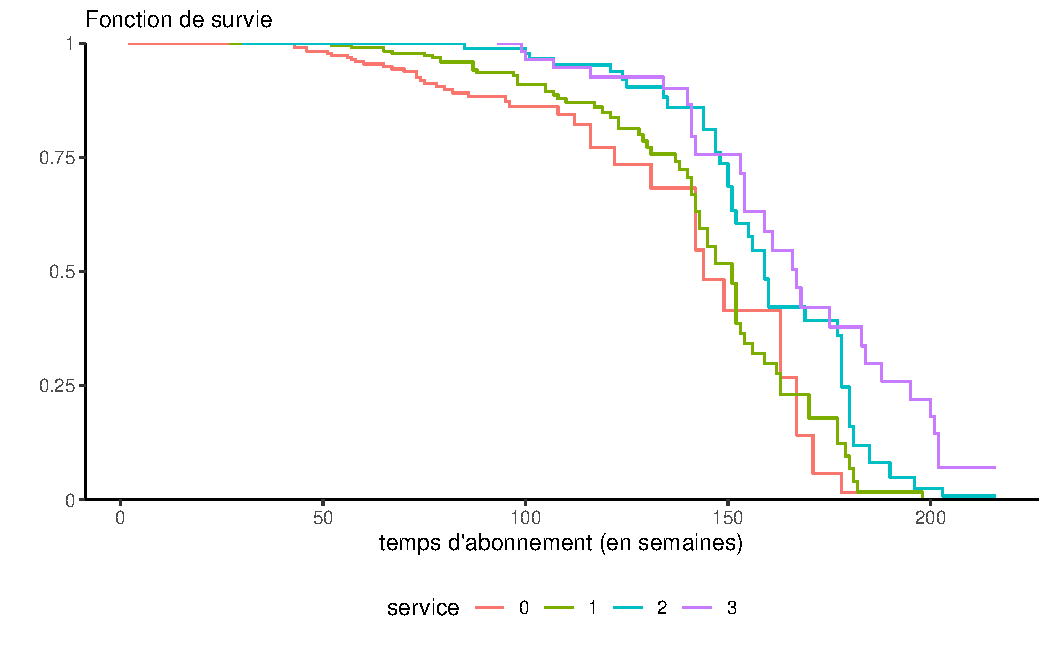
\includegraphics[width=0.85\textwidth,height=\textheight]{survie_files/figure-pdf/fig-courbesurviesstrat-1.pdf}

}

\caption{\label{fig-courbesurviesstrat}Courbes de survie estimées par
nombre de service pour le modèle de Cox avec stratification pour un
homme de 40 ans.}

\end{figure}%

\subsection{Modèle non-proportionnel}\label{moduxe8le-non-proportionnel}

Pour simplifier l'exposition, supposons que nous avons une seule
variable explicative \(X\). L'équation du modèle à risques
proportionnels est \(h(t; x) = h_0(t)\exp(\beta x)\) et suppose que la
fonction de risque de base \(h_0(t)\) est indépendante de la variable
explicative \(X\). Une manière de modéliser la non-proportionnalité est
d'inclure un terme d'interaction entre la variable et le temps. Il
existe plusieurs façons de le faire. Par exemple, on pourrait inclure
une nouvelle variable qui est le produit entre le temps et la variable
\(X\). Le modèle est alors \begin{align*}
h(t; x) = h_0(t) \exp(\beta_1x + \beta_2xt).
\end{align*} Pour ce modèle, le rapport de risque, pour une augmentation
d'une unité de \(X\) est \(\exp(\beta_1+ \beta_2t)\) et dépend du temps
\(t\): c'est un modèle avec risques non proportionnels. On retombe sur
le modèle à risques proportionnels lorsque \(\beta_2=0\).

Supposons que l'effet du nombre de service augmente avec le temps. On
peut inclure à la fois \texttt{service}, qui capture l'effet au temps
zéro, et le surenchérissement ou la diminution à mesure que le temps
d'abonnement progresse.

\begin{Shaded}
\begin{Highlighting}[]
\CommentTok{\# Créer variables binaires par service}
\NormalTok{survie1\_modif }\OtherTok{\textless{}{-}}\NormalTok{ survie1 }\SpecialCharTok{|\textgreater{}}
\NormalTok{  dplyr}\SpecialCharTok{::}\FunctionTok{mutate}\NormalTok{(}\AttributeTok{service1 =}\NormalTok{ service }\SpecialCharTok{==} \DecValTok{1}\NormalTok{,}
                \AttributeTok{service2 =}\NormalTok{ service }\SpecialCharTok{==} \DecValTok{2}\NormalTok{,}
                \AttributeTok{service3 =}\NormalTok{ service }\SpecialCharTok{==} \DecValTok{3}\NormalTok{)}
\NormalTok{cox\_np }\OtherTok{\textless{}{-}}\NormalTok{ survival}\SpecialCharTok{::}\FunctionTok{coxph}\NormalTok{(}
    \FunctionTok{Surv}\NormalTok{(temps, censure) }\SpecialCharTok{\textasciitilde{}} 
\NormalTok{     age }\SpecialCharTok{+}\NormalTok{ sexe }\SpecialCharTok{+}\NormalTok{ service }\SpecialCharTok{+} 
      \FunctionTok{tt}\NormalTok{(service1) }\SpecialCharTok{+} \FunctionTok{tt}\NormalTok{(service2) }\SpecialCharTok{+} \FunctionTok{tt}\NormalTok{(service3), }
     \AttributeTok{data =}\NormalTok{ survie1\_modif, }
     \AttributeTok{tt =} \ControlFlowTok{function}\NormalTok{(x, t, ...)\{t }\SpecialCharTok{*}\NormalTok{ x\})}
\end{Highlighting}
\end{Shaded}

Le bloc code précédent illustre comment créer le terme non
proportionnel: on spécifie avec l'option \texttt{tt()} la variable qui
change dans le temps et on spécifie par la suite la nature de
l'interaction temporelle en définissant une fonction \texttt{tt}.

Les variables catégorielles n'étant pas supportées en l'état, elles
doivent préalablement être transformées en variable indicatrices
binaires. Une fois les nouvelles variables dans la base de données, on
procède à la spécification du terme de risque non proportionnel.

\begin{longtable}[t]{lrrl}

\caption{\label{tbl-coxnph}Rapport de risque et intervalles de confiance
à niveau 95\% pour le modèle à risques non proportionnels (interaction
linéaire entre temps et service).}

\tabularnewline

\toprule
terme & exp(coef) & test de Wald & valeur-p\\
\midrule
age & 0.953 & -7.37 & <0.001\\
sexe & 0.543 & -5.24 & <0.001\\
service1 & 0.144 & -4.29 & <0.001\\
service2 & 0.072 & -3.76 & <0.001\\
service3 & 0.010 & -4.14 & <0.001\\
\addlinespace
tt(service1) & 1.010 & 2.17 & 0.0298\\
tt(service2) & 1.010 & 1.58 & 0.1132\\
tt(service3) & 1.023 & 2.48 & 0.0133\\
\bottomrule

\end{longtable}

Le Tableau~\ref{tbl-coxnph} contient les résultats. Les coefficients
pour l'interaction avec \(t\) sont petits, mais c'est parce que la
variable temps n'est pas standardisée et qu'elle s'étend de 0 à 200
semaines: de petites variations sont possiblement importantes quand le
temps augmente. Les estimations des coefficients pour l'interaction sont
tous positifs, ce qui suppose que le risque augmente avec le temps. Si
on considère comme source plausible d'effet du nombre de services un
quelconque rabais, il semble que cet effet protecteur s'amenuise. Deux
des termes d'interaction sont significatifs à niveau 5\% (statistiques
de Wald \(Z\) de 2.173, 1.584 et 2.476 et valeurs-\(p\) correspondantes
de 0.03, 0.113 et 0.013).

On peut aussi utiliser la structure de modèle à risques
non-proportionnels pour capturer l'effet des changements qui
interviennent au sein de variables explicatives dans le temps. Par
exemple, l'âge de la personne (en années) augmente à mesure que le temps
d'abonnement (en semaines) passe, d'où
\(\texttt{age}(t) = \texttt{age} + t/52\).

\begin{Shaded}
\begin{Highlighting}[]
\CommentTok{\# interaction entre service et temps}
\CommentTok{\# objet avec \textquotesingle{}tt\textquotesingle{} varie dynamiquement}
\NormalTok{cox6 }\OtherTok{\textless{}{-}} \FunctionTok{coxph}\NormalTok{(}
    \FunctionTok{Surv}\NormalTok{(temps, censure) }\SpecialCharTok{\textasciitilde{}} 
     \FunctionTok{tt}\NormalTok{(age) }\SpecialCharTok{+}\NormalTok{ sexe }\SpecialCharTok{+}\NormalTok{ service, }
     \AttributeTok{data =}\NormalTok{ survie1, }
     \AttributeTok{tt =} \ControlFlowTok{function}\NormalTok{(x, t, ...)\{x }\SpecialCharTok{+}\NormalTok{ t}\SpecialCharTok{/}\DecValTok{52}\NormalTok{\})}
\FunctionTok{summary}\NormalTok{(cox6)}
\end{Highlighting}
\end{Shaded}

On inclut uniquement la variable transformée \texttt{tt(age)} et son
effet est toujours fortement significatif pour expliquer le
désabonnement potentiel: les personnes plus âgées sont moins
susceptibles de résilier leur abonnement.

\begin{Shaded}
\begin{Highlighting}[]
\NormalTok{cox\_np }\OtherTok{\textless{}{-}}\NormalTok{ survival}\SpecialCharTok{::}\FunctionTok{coxph}\NormalTok{(}
    \FunctionTok{Surv}\NormalTok{(temps, censure) }\SpecialCharTok{\textasciitilde{}} 
     \FunctionTok{tt}\NormalTok{(age) }\SpecialCharTok{+}\NormalTok{ sexe }\SpecialCharTok{+}\NormalTok{ service, }
     \AttributeTok{data =}\NormalTok{ survie1, }
     \AttributeTok{tt =} \ControlFlowTok{function}\NormalTok{(x, t, ...)\{x }\SpecialCharTok{+}\NormalTok{ t}\SpecialCharTok{/}\DecValTok{52}\NormalTok{\})}
\FunctionTok{summary}\NormalTok{(cox\_np)}
\end{Highlighting}
\end{Shaded}

On spécifie avec l'option \texttt{tt()} dans la formule la variable qui
change dans le temps et par la suite la nature de l'interaction
temporelle avec l'argument \texttt{tt}.

\begin{longtable}[t]{lrrr}

\caption{\label{tbl-cox-np}Rapport de risque et intervalles de confiance
à niveau 95\% pour le modèle à risques non proportionnels (interaction
linéaire entre temps et âge).}

\tabularnewline

\toprule
terme & exp(coef) & borne inf. & borne sup.\\
\midrule
age & 0.91 & 0.87 & 0.95\\
tt(age) & 1.00 & 1.00 & 1.00\\
sexe & 0.52 & 0.41 & 0.65\\
region2 & 0.70 & 0.48 & 1.02\\
region3 & 1.03 & 0.73 & 1.46\\
\addlinespace
region4 & 0.80 & 0.56 & 1.12\\
region5 & 0.97 & 0.69 & 1.37\\
service1 & 0.36 & 0.28 & 0.46\\
service2 & 0.18 & 0.12 & 0.26\\
service3 & 0.12 & 0.07 & 0.20\\
\bottomrule

\end{longtable}

L'interaction employée ici n'est pas la seule fonction du temps qu'on
pourrait spécifier: on pourrait par exemple inclure une fonction de type
escalier \(\mathrm{I}(T< t_0)\) qui indique que l'effet de la variable
disparaît après le temps \(t_0\), si par exemple un rabais disparaît
après une certaine durée d'abonnement, avec
\texttt{rabais\ *\ I(t\textless{}t0)} pour une valeur numérique
\texttt{t0} fixée.

\section{Modèle à risques
compétitifs}\label{moduxe8le-uxe0-risques-compuxe9titifs}

Parfois, la raison pour laquelle un individu quitte l'état étudié peut
avoir un intérêt en soi. Par exemple si on s'intéresse au temps qu'un
employé demeure au service de la compagnie, la distinction entre le fait
qu'il ait démissionné ou bien qu'il ait été renvoyé peut avoir un impact
sur l'effet des variables explicatives. Comme autre exemple, si on
s'intéresse au temps de survie d'un individu après qu'il ait été
diagnostiqué avec un certain type de cancer, il pourrait être important
de distinguer selon la cause exacte de la mort.

De manière générale, supposons qu'il y a \(K\) manières possibles que
l'événement survienne.

\begin{figure}[ht!]

\centering{

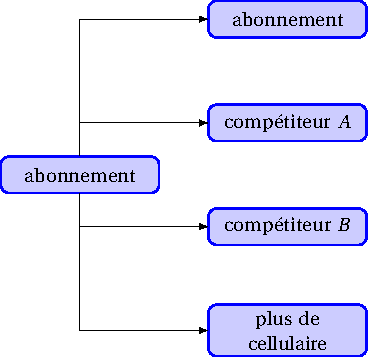
\includegraphics[width=0.65\textwidth,height=\textheight]{figures/transition_etats_modele_risque_competitifs.pdf}

}

\caption{\label{fig-transitionetat}Schéma illustrant la transition entre
état de base et autres événements compétitifs.}

\end{figure}%

Dans notre exemple d'abonnement cellulaire, supposons que nous avons
trois causes possibles pour la perte d'un client: soit il a interrompu
son abonnement pour aller chez le compétiteur A, soit pour aller chez le
compétiteur B, soit il n'a plus de cellulaire du tout. On considère un
modèle avec transition d'un état de base (abonné) vers un état absorbant
(désabonnement, soit chez compétiteur \(A\), compétiteur \(B\) ou
abandon du cellulaire).

On a deux avenues pour l'estimation de ce type de modèle: soit on ajuste
un modèle de Kaplan--Meier, soit un modèle de Cox.

On peut alors spécifier \(K\) fonctions de risques (une pour chaque
manière) et obtenir le modèle de Cox à risques compétitifs
(\emph{competing risks}), \begin{align*}
h_1(t; \boldsymbol{x})&= h_{01}(t) \exp(\beta_{11}x_1 + \cdots + \beta_{p1} x_p)\\
&\vdots\\
h_K(t; \boldsymbol{x})&= h_{0K}(t) \exp(\beta_{1K}x_1 + \cdots + \beta_{pK} x_p)\\
\end{align*} Notez que les coefficients sont différents d'une équation à
l'autre. En estimant ce modèle, on obtient donc une estimation de
l'effet des variables selon la raison du départ de l'état. De plus, on
peut aussi inclure des variables dont la valeur change dans le temps,
comme vu précédemment.

Ce qui simplifie énormément la situation est qu'il est prouvé qu'on peut
estimer les paramètres de chaque équation séparément sans perte de
précision. Par conséquent, en pratique, il suffira d'ajuster \(K\)
modèles de Cox séparément.

Les données pour cet exemple se trouvent dans le fichier
\texttt{survie4}. La seule nouveauté par rapport au fichier original est
la variable \(\texttt{censure}\) qui est maintenant codée ainsi

\begin{itemize}
\tightlist
\item
  1, si le temps est censuré (l'individu est toujours abonné à notre
  service)
\item
  2, si l'individu a quitté pour aller chez le compétiteur A
\item
  3, si l'individu a quitté pour aller chez le compétiteur B
\item
  4, si l'individu a quitté parce qu'il n'a plus besoin de cellulaire.
\end{itemize}

On peut calculer la fréquence de chaque modalité avec \texttt{table}.
Ainsi, il y a donc 166 clients toujours abonnés, 170 qui nous ont quitté
pour aller chez A, 121 pour aller chez B, et 43 qui n'ont plus de
cellulaires.

Pour ajuster le modèle lorsque la cause du départ est le compétiteur A,
le code définit \texttt{censure\ ==\ 2}.

\begin{Shaded}
\begin{Highlighting}[]
\CommentTok{\# Rappel pour \textasciigrave{}event\textasciigrave{}:}
\CommentTok{\#   1 pour observation, }
\CommentTok{\#   0 pour censure à droite}
\CommentTok{\# On utilise la convention TRUE = 1, FALSE = 0}
\FunctionTok{data}\NormalTok{(survie4, }\AttributeTok{package =} \StringTok{"hecmulti"}\NormalTok{)}
\NormalTok{cox5 }\OtherTok{\textless{}{-}} \FunctionTok{coxph}\NormalTok{(}\FunctionTok{Surv}\NormalTok{(}\AttributeTok{time =}\NormalTok{ temps, }
                   \AttributeTok{event =}\NormalTok{ censure }\SpecialCharTok{==} \DecValTok{2}\NormalTok{,}
                   \AttributeTok{type =} \StringTok{"right"}\NormalTok{) }\SpecialCharTok{\textasciitilde{}} 
\NormalTok{                age }\SpecialCharTok{+}\NormalTok{ sexe }\SpecialCharTok{+}\NormalTok{ region }\SpecialCharTok{+}\NormalTok{ service, }
              \AttributeTok{data =}\NormalTok{ survie4,}
              \AttributeTok{ties =} \StringTok{"exact"}\NormalTok{)}
\FunctionTok{summary}\NormalTok{(cox5)}
\end{Highlighting}
\end{Shaded}

\begin{longtable}[t]{lrrr}

\caption{\label{tbl-cox-risquecompetA}Rapport de risque et intervalles
de confiance à niveau 95\% pour le modèle à risques compétitifs
(probabilité de quitter pour compétiteur A).}

\tabularnewline

\toprule
terme & exp(coef) & borne inf. & borne sup.\\
\midrule
age & 0.95 & 0.94 & 0.97\\
sexe & 0.44 & 0.32 & 0.62\\
region2 & 0.54 & 0.32 & 0.92\\
region3 & 0.82 & 0.50 & 1.35\\
region4 & 0.72 & 0.45 & 1.16\\
\addlinespace
region5 & 1.05 & 0.66 & 1.66\\
service1 & 0.38 & 0.27 & 0.54\\
service2 & 0.18 & 0.11 & 0.30\\
service3 & 0.11 & 0.05 & 0.22\\
\bottomrule

\end{longtable}

Notez qu'on précise que les valeurs 1, 3 et 4 sont des observations
censurées. Ici, l'événement d'intérêt est que le client est parti chez
le compétiteur A. S'il est toujours abonné (\(\texttt{censure=1}\)),
s'il est parti chez le compétiteur B (\(\texttt{censure=3}\)) ou s'il
nous a quitté car il n'a plus de cellulaire (\(\texttt{censure=4}\)),
alors l'événement « quitter pour aller chez A » n'est pas survenu. C'est
pourquoi on doit traiter ces situations comme des censures.

Ainsi, on voit que l'événement est survenu 170 fois et qu'il y a 330
censures. L'interprétation des paramètres se fait comme précédemment.
Sauf qu'il faut préciser qu'il s'agit du risque de quitter pour aller
chez le compétiteur A. Par exemple, le risque de quitter pour aller chez
le compétiteur A d'une femme est 0.444 fois le risque de quitter pour
aller chez le compétiteur A d'un homme. Ainsi, les femmes sont moins à
risque de quitter pour aller chez le compétiteur A que les hommes.

Dans \textbf{R}, on peut aussi ajuster simultanément tous les modèles en
spécifiant que l'événement d'intérêt est un facteur: c'est alors la
catégorie de référence qui fait foi de l'état de départ. Il faut
également une variable qui identifie l'observation --- dans le cas qu'on
considère, c'est simplement une colonne avec des valeurs de \(1\) à
\(n\).

\begin{Shaded}
\begin{Highlighting}[]
\NormalTok{rc\_cox }\OtherTok{\textless{}{-}} \FunctionTok{coxph}\NormalTok{(}
  \FunctionTok{Surv}\NormalTok{(}\AttributeTok{time =}\NormalTok{ temps, }
       \AttributeTok{event =} \FunctionTok{factor}\NormalTok{(censure)) }\SpecialCharTok{\textasciitilde{}}\NormalTok{ sexe }\SpecialCharTok{+}\NormalTok{ age }\SpecialCharTok{+}\NormalTok{ service,}
  \AttributeTok{data =}\NormalTok{ survie4 }\SpecialCharTok{|\textgreater{}}
\NormalTok{    dplyr}\SpecialCharTok{::}\FunctionTok{mutate}\NormalTok{(}\AttributeTok{id =} \DecValTok{1}\SpecialCharTok{:}\FunctionTok{nrow}\NormalTok{(survie4)),}
  \AttributeTok{id =}\NormalTok{ id)}
\end{Highlighting}
\end{Shaded}

On obtient l'ensemble des coefficients dans le tableau résumé, un pour
chaque événement compétitif autre que la référence.

Si on voulait ajuster le modèle de Kaplan--Meier, pour une transition
d'un état de base (abonné) vers un état dit absorbant (désabonnement,
soit chez compétiteur A ou B ou abandon du cellulaire), il faut
obligatoirement ajuster toutes les courbes simultanément. On ajustera le
modèle multi-état en spécifiant un facteur pour l'événement, où encore
une fois la catégorie de référence est abonnement (\texttt{censure=1}).

\begin{Shaded}
\begin{Highlighting}[]
\NormalTok{rc\_km }\OtherTok{\textless{}{-}} \FunctionTok{survfit}\NormalTok{(}\FunctionTok{Surv}\NormalTok{(}\AttributeTok{time =}\NormalTok{ temps, }
             \AttributeTok{event =} \FunctionTok{factor}\NormalTok{(censure)) }\SpecialCharTok{\textasciitilde{}} \DecValTok{1}\NormalTok{,}
             \AttributeTok{data =}\NormalTok{ survie4)}
\end{Highlighting}
\end{Shaded}

Les représentations graphiques pour le modèle à risque compétitif sont
légèrement différente. Si on dichotomise l'événement d'intérêt (survie
ou échec), il y a deux options possibles et la probabilité d'échec est
complémentaire à la survie. Avec plus d'un choix, on obtiendra un
graphique avec une estimation de la probabilité pour chaque modalité de
l'événement: la Figure~\ref{fig-competitif} montre ceci pour la sortie
du modèle de Cox et le modèle de Kaplan--Meier en ajoutant la courbe
correspondant à la probabilité de demeurer abonné.

\begin{figure}[ht!]

\centering{

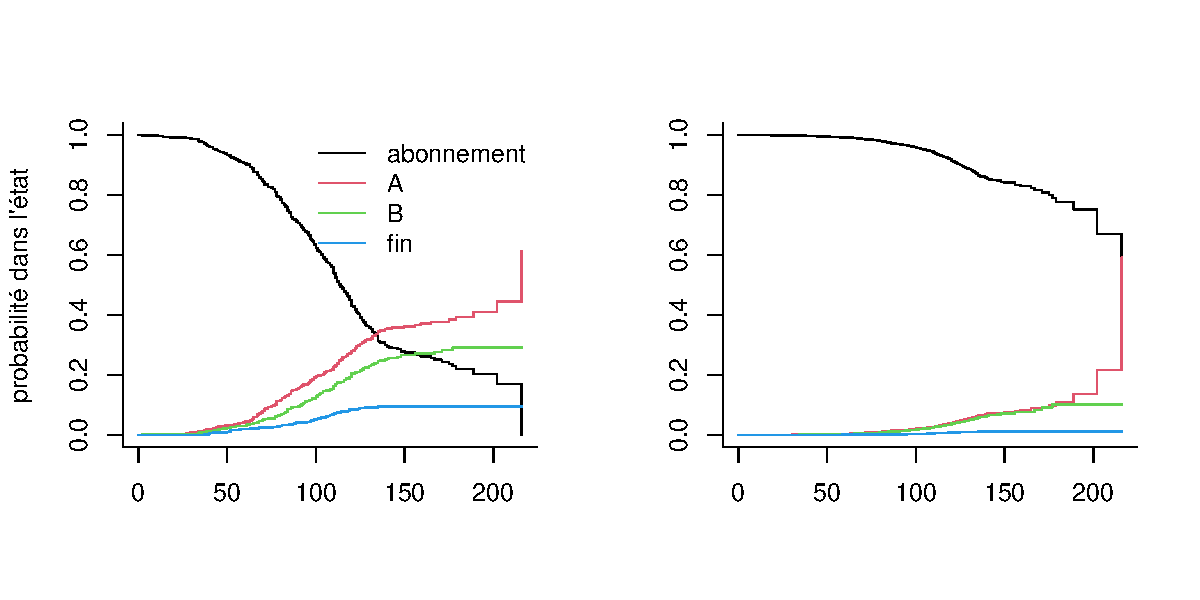
\includegraphics[width=0.9\textwidth,height=\textheight]{survie_files/figure-pdf/fig-competitif-1.pdf}

}

\caption{\label{fig-competitif}Probabilité d'événement sans variable
explicative (Kaplan-Meier, gauche) et avec âge, service et sexe (modèle
de Cox, droite).}

\end{figure}%

La
\href{https://cran.r-project.org/web/packages/survival/vignettes/timedep.pdf}{vignette}
du paquet \texttt{survival} offre des détails sur l'implémentation des
méthodes qui traitent de l'inclusion de variables explicatives dont la
valeur change dans le temps et sur les risques compétitifs.

\begin{tcolorbox}[enhanced jigsaw, bottomrule=.15mm, toptitle=1mm, opacityback=0, title=\textcolor{quarto-callout-note-color}{\faInfo}\hspace{0.5em}{En résumé}, left=2mm, bottomtitle=1mm, colbacktitle=quarto-callout-note-color!10!white, colback=white, breakable, toprule=.15mm, coltitle=black, arc=.35mm, opacitybacktitle=0.6, colframe=quarto-callout-note-color-frame, titlerule=0mm, leftrule=.75mm, rightrule=.15mm]

\begin{itemize}
\tightlist
\item
  Le modèle de Cox suppose qu'on peut diviser le risque en deux parties:
  le risque de base \(h_0(t)\) commun à tou(te)s (composante
  nonparamétrique) et l'effet multiplicatif
  \(\exp(\mathbf{X}\boldsymbol{\beta})\) (composante paramétrique)
\item
  Puisque la fonction de risque de base est commune à toutes les
  observations, moins d'incertitude sur l'estimation de la survie.
\item
  L'impact sur la survie de changement dans les variables explicatives
  n'est pas multiplicatif.
\item
  Le modèle de Cox suppose que le rapport de cote ne dépend pas du temps
  (postulat de risques proportionnels).
\item
  On peut vérifier ce postulat et généraliser le modèle au besoin.
\item
  Plutôt que d'inclure une variable catégorielle, on peut utiliser la
  stratification pour estimer le risque de base séparément sur chaque
  sous-groupe.
\item
  le modèle à risques non-proportionnels permet d'inclure une
  interaction entre le temps et une avec variable ou un coefficient.
\item
  Si les variables explicatives changent au fil du temps, on peut
  décomposer la contribution de l'observation en plusieurs segments.
\item
  Il y a un lien possible avec le modèle à risque proportionnels si
  l'effet est le même pour tous (comme l'âge).
\item
  Le modèle multi-état (modèle à risques compétitifs) permet d'estimer
  la probabilité de chaque transition: la survie pour l'événement de
  base reste le même (désabonnement), mais on décompose la probabilité
  de la censure selon les différents événements compétitifs.
\end{itemize}

\end{tcolorbox}

\bookmarksetup{startatroot}

\chapter{Réduction de la dimension}\label{analyse-factorielle}

\section{Introduction}\label{introduction-3}

Ce chapitre traite de réduction de la dimensionalité d'un problème
d'analyse multidimensionnelle. On dispose de \(p\) variables
\(X_1, \ldots, X_p\): comment résumer cet ensemble avec moins de
variables (disons \(k\)) tout en conservant le plus de variabilité
possible? Nous couvrons deux méthodes dans ce chapitre: la première,
intitulée \textbf{analyse en composantes principales}, cherche à
\textbf{réduire le nombre de variables explicatives} tout en préservant
le plus possible de variabilité exprimée et en créant de nouvelles
variables explicatives qui ne sont pas corrélées les unes avec les
autres.

La deuxième, appelée analyse factorielle exploratoire, cherche à
expliquer la structure de corrélation entre les \(p\) variables à l'aide
d'un nombre restreint de facteurs. Elle répond aux questions suivantes:

\begin{itemize}
\tightlist
\item
  Y a-t-il des groupements de variables?
\item
  Est-ce que les variables faisant partie d'un groupement semblent
  mesurer certains aspects d'un facteur commun (non observé)?
\end{itemize}

De tels groupements peuvent être détecté si plusieurs variables sont
très corrélées entre elles. Une analyse factorielle cherchera à
identifier automatiquement ces groupes de variables.

Les facteurs sont des variables latentes qui mesurent des constructions.
Par exemple, l'habileté quantitative, l'habileté sociale, l'importance
accordée à la qualité du service, l'importance accordée à la loyauté,
l'habileté de leader, etc.

L'analyse factorielle est aussi une méthode de réduction du nombre de
variables. En effet, une fois qu'on a identifié les facteurs, on peut
remplacer les variables individuelles par un résumé pour chaque facteur
(qui est souvent la moyenne des variables qui font partie du facteur).

\section{Coefficient de corrélation
linéaire}\label{coefficient-de-corruxe9lation-linuxe9aire}

On veut examiner la relation entre deux variables \(X_j\) et \(X_k\) et
on dispose de \(n\) couples d'observations, où \(x_{i, j}\)
(respectivement \(x_{i, k}\)) est la valeur de la variable \(X_j\)
(\(X_k\)) pour la \(i\)e observation.

Le coefficient de corrélation linéaire entre \(X_j\) et \(X_k\), que
l'on note \(r_{j, k}\), cherche à mesurer la force de la relation
linéaire entre deux variables, c'est-à-dire à quantifier à quel point
les observations sont alignées autour d'une droite. Le coefficient de
corrélation est \begin{align*}
r_{j, k} &= \frac{\widehat{\mathsf{Co}}(X_j, X_k)}{\{\widehat{\mathsf{Va}}(X_j) \widehat{\mathsf{Va}}(X_k)\}^{1/2}} 
%\\&=\frac{\sum_{i=1}^n (x_{i, j}-\overline{x}_j)(x_{i, k} -\overline{x}_{k})}{\left\{\sum_{i=1}^n (x_{i, j}-\overline{x}_j)^2 \sum_{i=1}^n(x_{i, k} -\overline{x}_{k})^2\right\}^{1/2}}
\end{align*}

Les propriétés les plus importantes du coefficient de corrélation
linéaire \(r\) sont les suivantes:

\begin{enumerate}
\def\labelenumi{\arabic{enumi})}
\tightlist
\item
  \(-1 \leq r \leq 1\);
\item
  \(r=1\) (respectivement \(r=-1\)) si et seulement si les \(n\)
  observations sont exactement alignées sur une droite de pente positive
  (négative). C'est-à-dire, s'il existe deux constantes \(a\) et \(b>0\)
  (\(b<0\)) telles que \(y_i=a+b x_i\) pour tout \(i=1, \ldots, n\).
\end{enumerate}

Règle générale,

\begin{itemize}
\tightlist
\item
  Le signe de la corrélation détermine l'orientation de la pente
  (négative ou positive)
\item
  Plus la corrélation est près de 1 en valeur absolue, plus les points
  auront tendance à être alignés autour d'une droite.
\item
  Lorsque la corrélation est presque nulle, les points n'auront pas
  tendance à être alignés autour d'une droite. Il est très important de
  noter que cela n'implique pas qu'il n'y a pas de relation entre les
  deux variables. Cela implique seulement qu'il n'y a pas de
  \textbf{relation linéaire} entre les deux variables. La
  Figure~\ref{fig-datasaurus} montre bien ce point: ces jeux de données
  ont la même corrélation linéaire (quasi-nulle), mais ne sont
  clairement pas indépendantes puisqu'elles permettent de dessiner un
  dinosaure ou une étoile.
\end{itemize}

\begin{figure}[ht!]

\centering{

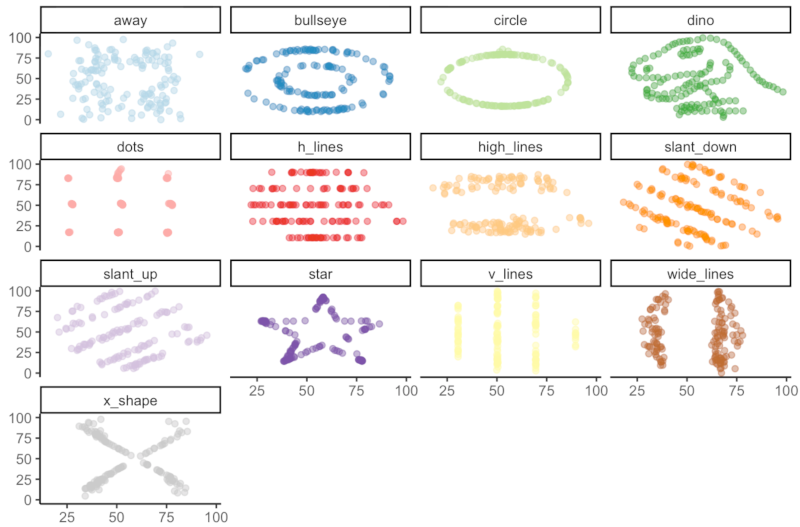
\includegraphics{figures/DataSaurusDozen.png}

}

\caption{\label{fig-datasaurus}Datasaurus (Alberto Cairo): une douzaine
de jeux de données qui ont les mêmes statistiques descriptives (à deux
décimales près) et une faible corrélation, mais qui sont visuellement
distincts.}

\end{figure}%

La matrice de corrélation entre \(X_1, \ldots, X_p\), dont l'entrée
\((i, j)\) contient la corrélation entre \(X_i\) et \(X_j\), est une
matrice symmétrique dont les éléments de la diagonale sont égaux à 1. À
mesure que le nombre de variables augmente, le nombre de corrélations à
estimer augmente: puisque la matrice est \(p \times p\), ce nombre
augmente comme le carré du nombre de variables explicatives.
L'estimation ne sera pas fiable à moins que \(n \gg p\).

\section{Présentation des
données}\label{pruxe9sentation-des-donnuxe9es-1}

Le questionnaire suivant porte sur une étude dans un magasin. Pour les
besoins d'une enquête, on a demandé à 200 consommateurs adultes de
répondre aux questions suivantes par rapport à un certain type de
magasin sur une échelle de 1 à 5, où

\begin{enumerate}
\def\labelenumi{\arabic{enumi}.}
\tightlist
\item
  pas important
\item
  peu important
\item
  moyennement important
\item
  assez important
\item
  très important
\end{enumerate}

Pour vous, à quel point est-ce important\ldots

\begin{enumerate}
\def\labelenumi{\arabic{enumi}.}
\tightlist
\item
  que le magasin offre de bons prix tous les jours?
\item
  que le magasin accepte les cartes de crédit majeures (Visa,
  Mastercard)?
\item
  que le magasin offre des produits de qualité?
\item
  que les vendeurs connaissent bien les produits?
\item
  qu'il y ait des ventes spéciales régulièrement?
\item
  que les marques connues soient disponibles?
\item
  que le magasin ait sa propre carte de crédit?
\item
  que le service soit rapide?
\item
  qu'il y ait une vaste sélection de produits?
\item
  que le magasin accepte le paiement par carte de débit?
\item
  que le personnel soit courtois?
\item
  que le magasin ait en stock les produits annoncés?
\end{enumerate}

Les statistiques descriptives ainsi que la matrice des corrélations sont
obtenues en exécutant les lignes suivantes:

\begin{Shaded}
\begin{Highlighting}[]
\FunctionTok{data}\NormalTok{(factor, }\AttributeTok{package =} \StringTok{"hecmulti"}\NormalTok{)}
\CommentTok{\# Matrice de corrélation}
\FunctionTok{cor}\NormalTok{(factor)}
\CommentTok{\# Statistiques descriptives}
\FunctionTok{summary}\NormalTok{(factor)}
\end{Highlighting}
\end{Shaded}

\begin{longtable}[t]{lrrrrrrrrrrrr}

\caption{\label{tbl-corrmat}Matrice de corrélation de \texttt{factor}.}

\tabularnewline

\toprule
 & x1 & x2 & x3 & x4 & x5 & x6 & x7 & x8 & x9 & x10 & x11 & x12\\
\midrule
x1 &  & -0.08 & -0.14 & -0.07 & 0.38 & -0.01 & -0.10 & -0.13 & -0.03 & -0.11 & -0.12 & -0.01\\
x2 &  &  & 0.04 & -0.02 & -0.08 & 0.06 & 0.50 & 0.01 & -0.01 & 0.43 & -0.12 & 0.07\\
x3 &  &  &  & 0.10 & -0.06 & 0.39 & 0.00 & 0.05 & 0.47 & 0.08 & 0.13 & 0.46\\
x4 &  &  &  &  & -0.05 & 0.06 & 0.08 & 0.57 & 0.01 & 0.09 & 0.50 & 0.09\\
x5 &  &  &  &  &  & -0.04 & -0.04 & -0.02 & 0.03 & -0.07 & -0.06 & -0.07\\
\addlinespace
x6 &  &  &  &  &  &  & 0.07 & 0.04 & 0.32 & 0.07 & -0.04 & 0.32\\
x7 &  &  &  &  &  &  &  & 0.09 & -0.02 & 0.51 & -0.03 & 0.02\\
x8 &  &  &  &  &  &  &  &  & -0.03 & 0.16 & 0.55 & 0.04\\
x9 &  &  &  &  &  &  &  &  &  & 0.01 & 0.02 & 0.39\\
x10 &  &  &  &  &  &  &  &  &  &  & 0.01 & 0.02\\
\addlinespace
x11 &  &  &  &  &  &  &  &  &  &  &  & 0.05\\
x12 &  &  &  &  &  &  &  &  &  &  &  & \\
\bottomrule

\end{longtable}

\begin{figure}[ht!]

\centering{

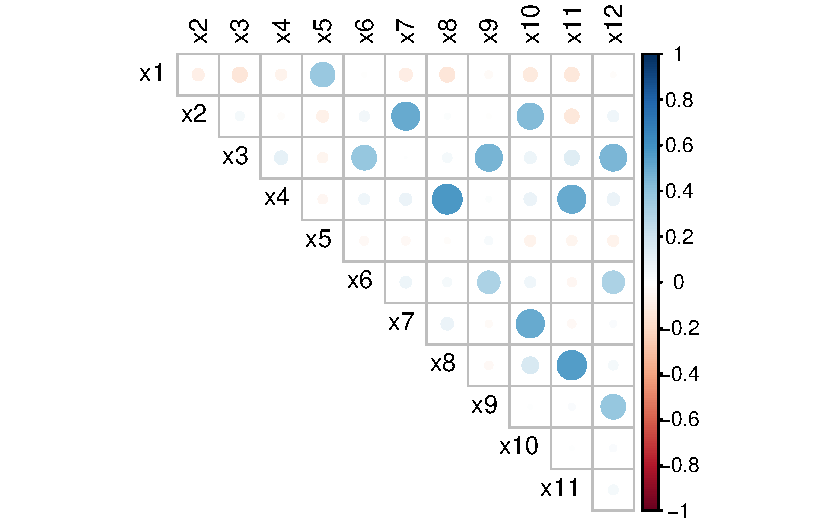
\includegraphics[width=0.8\textwidth,height=\textheight]{analysefactorielle_files/figure-pdf/fig-corrmat-1.pdf}

}

\caption{\label{fig-corrmat}Corrélogramme de la base de données
\texttt{factor}.}

\end{figure}%

\begin{table}

\caption{\label{tbl-statdescriptfactorpdf}Statistiques descriptives des
12 variables du jeu de données factor.}

\centering{

\centering
\begin{tabular}[t]{rrrr}
\toprule
moyenne & écart-type & min & max\\
\midrule
2.26 & 1.13 & 1 & 5\\
2.51 & 1.24 & 1 & 5\\
3.00 & 1.19 & 1 & 5\\
2.91 & 1.33 & 1 & 5\\
3.55 & 1.17 & 1 & 5\\
\addlinespace
2.14 & 1.14 & 1 & 5\\
1.82 & 1.06 & 1 & 5\\
2.92 & 1.32 & 1 & 5\\
3.04 & 1.12 & 1 & 5\\
2.59 & 1.32 & 1 & 5\\
\addlinespace
2.98 & 1.33 & 1 & 5\\
3.45 & 1.16 & 1 & 5\\
\bottomrule
\end{tabular}

}

\end{table}%

On voit dans la Figure~\ref{fig-corrmat} que quelques groupes de
variables sont corrélés entre eux. On peut également regrouper certaines
questions sous des thèmes manuellement: le but de l'analyse factorielle
sera d'automatiser ce regroupement.

\section{Analyse en composantes
principales}\label{analyse-en-composantes-principales}

Le but de l'analyse en composantes principales est de réduire le nombre
de variables explicatives. En partant de \(p\) variables
\(X_1, \ldots, X_p\), on forme de nouvelles variables qui sont des
combinaisons linéaires des variables originales, \begin{align*}
C_j &= \underset{\text{somme de poids fois variables explicatives}}{w_{j1} X_1 + w_{j2} X_2 + \cdots + w_{jp} X_p}, \qquad (j=1, \ldots, p),
\\
1 &= \underset{\text{poids standardisés}}{w_{j1}^2 + \cdots + w_{jp}^2}
\end{align*} de telle sorte que

\begin{itemize}
\tightlist
\item
  La première variable formée, \(C_1\), appelée première composante
  principale, possède la variance maximale parmi toutes les combinaisons
  linéaires sous la contrainte
  \(w_{1i}^2 + \cdots + w_{1p}^2=1\).\footnote{Les contraintes sur les
    poids sont nécessaires afin de standardiser le problème car il
    serait possible d'avoir des variances infinies sinon.}
\item
  Pour \(j=2, \ldots, p\), la \(j\)e composante principale \(C_j\)
  possède la variance maximale parmi toutes les combinaisons linéaires
  qui sont non corrélées avec \(C_1, \ldots, C_{j-1}\) sous la
  contrainte \(w_{j1}^2 + \cdots + w_{jp}^2=1\).
\end{itemize}

Ainsi, les composantes principales forment un ensemble de variables non
corrélées entre elles, qui récupèrent en ordre décroissant le plus
possible de la variance des variables originales. La somme des variances
des \(p\) composantes principales est égale à la somme des variances des
\(p\) variables originales.

Mathématiquement, les composantes principales correspondent aux vecteurs
propres de la matrice de covariance, mais on peut également utiliser la
matrice de corrélation\footnote{La fonction \texttt{princomp} peut
  directement utiliser la base de données numériques, ou la matrice de
  covariance. Dans le premier cas, on peut spécifier que l'on veut la
  décomposition de la matrice de corrélation à l'aide de l'argument,
  \texttt{cor}}. L'avantage de la matrice de corrélation (ou de la
standardisation des variables) est que l'unité de mesure n'impacte pas
le résultat; autrement, un poids plus important est attribué aux
variables qui ont la plus forte hétérogénéité.

Si on conserve toutes les composantes principales, cela revient à
changer le système de coordonnées dans lequel sont exprimées nos
observations en effectuant une rotation: avec deux variables, on on
trouve la direction dans le système 2D dans lequel l'étendue est la plus
grande. Si une simple rotation peut sembler inutile, la méthode est fort
utile en haute dimension. On espère en général qu'un petit nombre de
composantes principales réussira à expliquer la plus grande partie de la
variance totale.

\begin{figure}[ht!]

\centering{

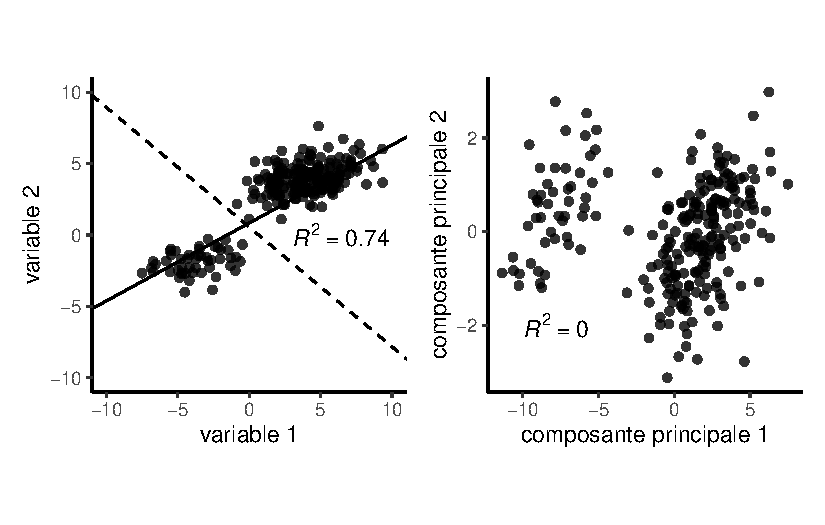
\includegraphics[width=0.9\textwidth,height=\textheight]{analysefactorielle_files/figure-pdf/fig-acprotation-1.pdf}

}

\caption{\label{fig-acprotation}Nuage de points avant (gauche) et après
(droite) analyse en composantes principales. Les directions des
composantes principales (lignes pleines et traitillés), qui forment un
angle droit, sont ajoutées au nuage de points à gauche. On peut
constater que la corrélation entre les deux composantes principales est
nulle.}

\end{figure}%

La Figure~\ref{fig-acprotation} démontre cette décomposition sur des
données bidimensionnelles simulées. La variance des données dans le
premier panneau est 13.51 pour l'axe des abscisse et 6.43 pour l'axe des
ordonnées avec une corrélation de 0.86, à comparer avec des variances de
18.65 et 1.21 et une corrélation nulle entre les deux composantes
principales.

Dans une analyse en composantes principales, on conservera un nombre
\(k<p\) de variables explicatives pour résumer les données. Ce outil est
utilisé à des fins exploratoires, puisqu'on n'implique pas de variable
réponse dans le modèle. L'analyse en composantes principales est utilisé
pour réduire la dimension afin de faire de la classification, de
l'analyse de regroupements et aussi réduire les coûts associés à ces
méthodes en projetant les données dans un sous-espace de dimension plus
faible.

En \textbf{R}, on effectue l'analyse en composantes principales avec la
fonction \texttt{princomp} ou \texttt{prcomp}\footnote{La différence
  entre les deux sorties est due à deux choses: \texttt{princomp}
  utilise la décomposition en valeurs propres avec
  \(n^{-1}\mathbf{X}^\top\mathbf{X}\) pour la matrice de covariance,
  tandis que \texttt{prcomp} utilise la décomposition en valeurs
  singulières avec un dénominateur de \(n-1\); cette dernière option est
  plus stable numériquement. On pourrait aussi utiliser
  \texttt{eigen(cor(factor))} pour extraire directement la décomposition
  en valeurs propres/vecteurs propres, mais on n'aurait pas accès aux
  méthodes pour la visualisation.}.

La sortie contient

\begin{itemize}
\tightlist
\item
  les coordonnées des composantes principales, \texttt{acp\$scores}; la
  première est celle qui a la plus grande variabilité.
\item
  l'écart-type de chaque composante, \texttt{acp\$sdev}. Chaque
  écart-type est la racine carrée d'une des valeurs propres.
\item
  les poids \(w_{ij}\), appelés chargements (\emph{loadings}), qui
  donnent la correspondance entre le système de coordonnées des
  composantes principales et celui des variables \(\boldsymbol{X}\)
  originales.
\end{itemize}

On peut représenter les données à l'aide d'un bigramme: c'est une nuage
de points de chaque observations dans l'espace des deux premières
composantes principales. Si on couple cela avec les directions offertes
par les chargements pour chacune des variables explicatives
\(X_1, \ldots, X_p\), il en ressort que certaines variables
augmentent/diminuent de pair. Ainsi, on voit dans la
Figure~\ref{fig-biplot} que les variables \texttt{x3}, \texttt{x6},
\texttt{x9} et \texttt{x12} tendent dans la même direction, comme
\texttt{x4}, \texttt{x8} et \texttt{x11}. On reviendra sur ce point dans
une section subséquente.

Une fois qu'on a choisit le nombre de composantes, on pourrait ne
conserver que les \(k\) premières colonnes de la matrice des composantes
principales \texttt{acp\$scores} pour faire les graphiques ou pour
approximer la matrice de covariance. Il faut garder en tête qu'il faudra
néanmoins collecter les mêmes questions pour recréer les composantes
principales avec de nouvelles observations, ce qui est peu commode si on
veut réduire le coût de la collecte.

\begin{Shaded}
\begin{Highlighting}[]
\CommentTok{\# Analyse en composantes principales}
\CommentTok{\# de la matrice de corrélation}
\NormalTok{acp }\OtherTok{\textless{}{-}} \FunctionTok{princomp}\NormalTok{(factor, }\AttributeTok{cor =} \ConstantTok{TRUE}\NormalTok{)}
\FunctionTok{loadings}\NormalTok{(acp) }\CommentTok{\# chargements}
\FunctionTok{biplot}\NormalTok{(acp) }\CommentTok{\# bigramme}
\end{Highlighting}
\end{Shaded}

\begin{figure}[ht!]

\centering{

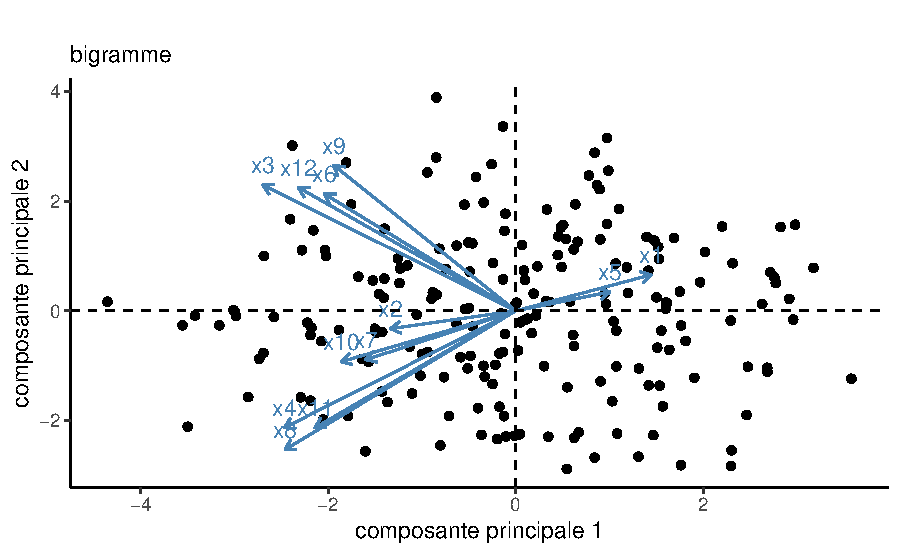
\includegraphics[width=0.6\textwidth,height=\textheight]{analysefactorielle_files/figure-pdf/fig-biplot-1.pdf}

}

\caption{\label{fig-biplot}Bigramme: nuage de point des coordonnées des
deux premières composantes principales et direction selon chargements
des variables explicatives originales.}

\end{figure}%

On peut étudier la sortie pour vérifier les propriétés de notre
décomposition. Le Tableau~\ref{tbl-eigenvalues} montre la variance de
chaque composante principale. Si on additionne l'ensemble des variances
(sans arrondir), on obtient une variance cumulative des 12 composantes
principales, 12, soit le même que le nombre de variables explicatives
puisque les variables standardisées ont variance unitaire. Si on calcule
la matrice de corrélation, \texttt{cor(acp\$scores)}, on remarquera que
la corrélation est nulle entre les variables.

\begin{longtable}[t]{cccccccccccc}

\caption{\label{tbl-eigenvalues}Variance des composantes principales}

\tabularnewline

\toprule
C1 & C2 & C3 & C4 & C5 & C6 & C7 & C8 & C9 & C10 & C11 & C12\\
\midrule
2.43 & 2.00 & 1.94 & 1.30 & 0.74 & 0.69 & 0.57 & 0.54 & 0.51 & 0.47 & 0.46 & 0.36\\
\bottomrule

\end{longtable}

\subsection{Choix du nombre de composantes
principales}\label{sec-acp-choix}

Si on désire réduire la dimension, il nous faudra choisir \(k \leq p\)
variables. Cette section traite du choix du nombre de variables
explicatives à retenir. Idéalement, ce nombre devrait être beaucoup plus
petit que le nombre original de variables.

Une première approche est de regarder le pourcentage de la variance
totale expliquée. Puisque les composantes principales sont ordonnées en
ordre décroissant de variance, on peut étudier la variance cumulative
des \(k\) premières composantes et choisir un nombre qui explique le
plus possible. Si l'ajout d'une variable augmente peu la variabilité
totale expliquée par l'ensemble, alors cette variable est probablement
superflue. On pourrait choisir un nombre de composantes pour expliquer
un pourcentage prédéfini de la vairance totale, disons 70\%. Deux autres
critères couramment employés sont:

\begin{itemize}
\tightlist
\item
  \textbf{critère du coude de Cattell}: ce critère consiste à
  sélectionner un nombre de composantes dans le diagramme d'éboulis
  (\texttt{screeplot}), un graphique des variances des composantes
  principales\footnote{Soit les valeurs propres de la matrice de
    covariance ou corrélation}. Habituellement, il y a une décroissance
  rapide de la variance suivie d'un plateau: on prendra le nombre de
  composantes qui correspond au \(k\) juste avant l'apparition du
  plateau (la valeur précédant le pli du coude). C'est un critère très
  subjectif, puisqu'il y a souvent plusieurs plateaux et que la variance
  peut décroître très lentement. On peut utiliser la fonction
  \texttt{screeplot} pour obtenir le diagramme d'éboulis mais il est
  facile de le créer manuellement et le résultat est esthétiquement plus
  réussi.
\item
  \textbf{critère des valeurs propres de Kaiser}: un critère basé sur
  les valeurs propres de la matrice de corrélation. Le nombre de
  facteurs choisis est le nombre de composantes principales dont la
  variance est supérieures à 1. L'idée est de garder seulement les
  facteurs qui expliquent plus de variance qu'une variable individuelle.
\end{itemize}

Si on utilise le critère de Kaiser avec les données \texttt{factor}, on
conservera 4 composantes principales qui expliqueront 63.9 pourcent de
la variance totale des variables originales - voir le
Tableau~\ref{tbl-eigenvalues}. Le diagramme d'éboulis de la
Figure~\ref{fig-screeplot}, qui peut être produit avec la fonction
\texttt{hecmulti::eboulis(eigen(cor(factor))} suggère quant à lui quatre
composantes.

\begin{figure}[ht!]

\centering{

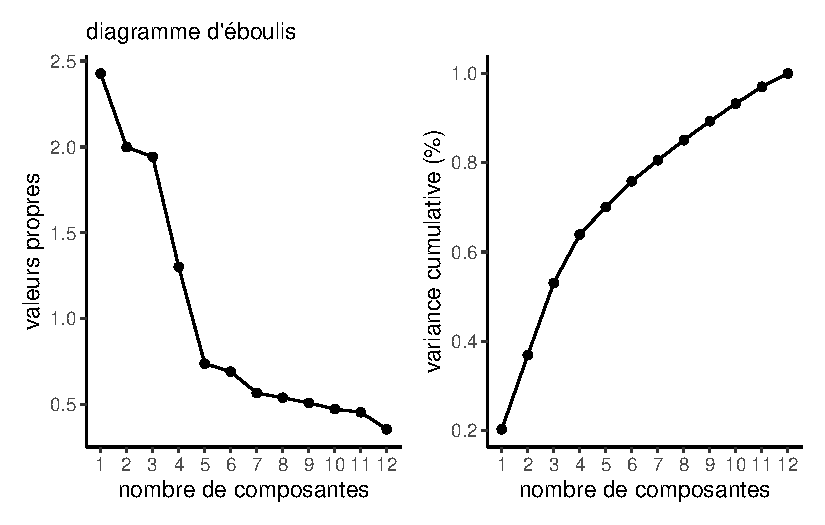
\includegraphics[width=0.85\textwidth,height=\textheight]{analysefactorielle_files/figure-pdf/fig-screeplot-1.pdf}

}

\caption{\label{fig-screeplot}Diagramme d'éboulis (gauche) représentant
la variance des composantes principales (en ordonnée) en fonction du
nombre composantes principales (en abscisse). Variance cumulative en
fonction du nombre de composantes principales (droite).}

\end{figure}%

Une fois qu'on a déterminé le nombre de facteurs, on peut extraire les
nouvelles variables explicatives à partir de l'analyse en composantes
principales. Les colonnes sont stockées dans \texttt{acp\$score} et il
suffit de conserver les premières colonnes.

\subsection{Formulation mathématique}\label{formulation-mathuxe9matique}

Ce complément d'information est optionnel.

Mathématiquement, le problème de l'analyse en composantes principales
revient à calculer la décomposition en valeurs propres et vecteurs
propres de la matrice de covariance
\(\mathsf{Co}(\boldsymbol{X})=\boldsymbol{\Sigma}\). On peut écrire
\begin{align*}
\boldsymbol{\Sigma} = \boldsymbol{Q}\boldsymbol{\Lambda}\boldsymbol{Q}^\top
\end{align*} où
\(\boldsymbol{\Lambda} = \mathrm{diag}\{\lambda_1, \ldots, \lambda_p\}\)
est une matrice diagonale contenant les valeurs propres en ordre
décroissant (\(\lambda_1 \geq \cdots \geq \lambda_p > 0\)) et
\(\boldsymbol{Q}\) est une matrice carrée \(p \times p\) orthogonale
contenant les vecteurs propres. La meilleure approximation de rang
\(k \leq p\) de \(\boldsymbol{\Sigma}\) est obtenue en spécifiant
\begin{align*}
\widetilde{\boldsymbol{\Sigma}}_k = \sum_{j=1}^k \lambda_j \boldsymbol{q}_j\boldsymbol{q}_j^\top,
\end{align*} une combinaison des vecteurs propres
\(\boldsymbol{q}_1, \ldots, \boldsymbol{q}_k \in \mathbb{R}^p\) non
corrélés.

\begin{tcolorbox}[enhanced jigsaw, bottomrule=.15mm, toptitle=1mm, opacityback=0, title=\textcolor{quarto-callout-note-color}{\faInfo}\hspace{0.5em}{En résumé}, left=2mm, bottomtitle=1mm, colbacktitle=quarto-callout-note-color!10!white, colback=white, breakable, toprule=.15mm, coltitle=black, arc=.35mm, opacitybacktitle=0.6, colframe=quarto-callout-note-color-frame, titlerule=0mm, leftrule=.75mm, rightrule=.15mm]

\begin{itemize}
\tightlist
\item
  La corrélation mesure la force de la dépendance linéaire entre deux
  variables: plus elle est élevée, plus les points s'alignent.
\item
  Si le nombre de variables explicatives \(p\) est conséquent par
  rapport au nombre d'observations \(n\), on a peu d'information
  disponible pour estimer de manière fiable les corrélations.
\item
  Une analyse en composante principales fait une décomposition en
  valeurs propres/vecteurs propres de la matrice de covariance ou de
  corrélation.

  \begin{itemize}
  \tightlist
  \item
    Ces nouvelles variables sont orthogonales (corrélation nulle) entre
    elles.
  \item
    Les composantes principales sont ordonnées en ordre décroissant de
    variance: si on ne conserve que \(k<p\) de variables, on maximise la
    variance expliquée.
  \item
    Le choix du nombre de variables est basé sur des règles du pouce: le
    critère des valeurs propres de Kaiser suggère de prendre autant de
    composantes principales que de variances supérieures à 1.
  \item
    Un bigramme permet de représenter graphiquement les directions des
    variables en fonction des deux premières composantes principales.
  \end{itemize}
\end{itemize}

\end{tcolorbox}

\section{Analyse factorielle
exploratoire}\label{analyse-factorielle-exploratoire-1}

Si le bigramme a permis de faire ressortir quelques orientations
communes, on aimerait aller plus loin dans notre exploration. On
considère encore une fois la matrice de covariance associée avec \(p\)
variables explicatives \(X_1, \ldots, X_p\): le modèle d'analyse
factorielle cherche à décrire cette dernière en fonction d'un plus petit
nombre de paramètres.

Conceptuellement, le modèle d'analyse factorielle suppose qu'on peut
regrouper les variables explicatives numériques (parfois avec quelques
variables binaires) à l'aide de concepts communs appelés facteurs.
Certaines variables explicatives devraient donc idéalement être
fortements corrélées entre elles. Le choix des variables est dicté par
le bon sens: on inclut dans le modèle des variables qui peuvent
logiquement être associée, par exemple des items de questionnaires
excluant les données sociodémographiques.

Le modèle d'analyse factorielle fait l'hypothèse que les variables
dépendent linéairement d'un plus petit nombre de variables aléatoires,
\(F_1, \ldots, F_m\), appelées facteurs communs. Cette relation n'est
pas parfaite, aussi on inclut \(p\) termes d'aléas
\(\varepsilon_1, \ldots, \varepsilon_p\), de moyenne zéro et de variance
\(\mathsf{Va}(\varepsilon_i)=\psi_i\) (\(i=1, \ldots, p\)). À des fins
d'identifiabilité, on suppose que les aléas ne sont pas corrélées aux
facteurs \(F\) et entre elles et que les facteurs \(F_1, \ldots, F_m\)
ont une moyenne nulle et une variance unitaire, donc
\(\mathsf{E}(F_i)=0\) et \(\mathsf{Va}(F_i)=1\) (\(i=1, \ldots, p\)).

Le modèle d'analyse factorielle s'écrit \begin{align*}
\boldsymbol{X} &= \underset{\text{moyenne}}{\boldsymbol{\mu}} + \underset{\text{combinaison linéaire de facteurs latents}}{\boldsymbol{\Gamma}\boldsymbol{F}} + \underset{\text{aléa}}{\boldsymbol{\varepsilon}},
\end{align*} ou si on écrit le système ligne par ligne, \begin{align*}
X_1 &= \mu_1 + \gamma_{11}F_1 + \gamma_{12} F_2 + \cdots + \gamma_{1m}F_m + \varepsilon_1\\
X_2 &= \mu_2 + \gamma_{21}F_1 + \gamma_{22} F_2 + \cdots + \gamma_{2m}F_m + \varepsilon_2\\
&\vdots \\
X_p &= \mu_p + \gamma_{p1}F_1 + \gamma_{p2} F_2 + \cdots + \gamma_{pm}F_m + \varepsilon_p, 
\end{align*} où \(\mu_i\) est l'espérance (moyenne théorique) de la
variable aléatoire \(X_i\), \(\boldsymbol{\Gamma}\) est une matrice
\(p \times m\) avec éléments \(\gamma_{ij}\), qui représentent le
chargement (poids) de la variable \(X_i\) sur le facteur \(F_j\)
(\(i=1, \ldots, p\); \(j=1, \ldots, m\)).

Les espérances (\(\mu_i\)), les chargements (\(\gamma_{ij}\)) et les
variances (\(\psi_i\)) sont des quantités fixes, mais inconnues, tandis
que les facteurs communs (\(F_i\)) et les aléas (\(\varepsilon_i\)) sont
des variables aléatoires non observables.

Selon ce modèle, on obtient \begin{align*}
\mathsf{Va}(\boldsymbol{X}) &= \boldsymbol{\Gamma}\mathsf{Va}(\boldsymbol{F})\boldsymbol{\Gamma}^\top + \mathsf{Va}(\boldsymbol{\varepsilon})\\
& = \boldsymbol{\Gamma}\boldsymbol{\Gamma}^\top + \mathrm{diag}(\boldsymbol{\psi}).
\end{align*} Les éléments diagonaux de cette matrice sont
\(\mathsf{Va}(X_j) = \sum_{l=1}^k \gamma_{jl}^2 + \psi_j\): on appelle
\textbf{communalité} le terme \(h_j = \sum_{l=1}^k \gamma_{jl}^2\), qui
représente la proportion de variance totale de \(X_j\) due à la
corrélation entre les facteurs. Le terme \(\psi_j\) est dénommé
\textbf{unicité}.

Si les variables ont été préalablement standardisées de telle sorte que
\(\mathsf{E}(X_i)=0\) et \(\mathsf{Va}(X_i)=1\) (ce qui revient à
utiliser la matrice de corrélation des observations dans l'analyse),
alors \(\mathsf{Cor}(X_i, F_j)=\gamma_{ij}\), c'est-à-dire, le
chargement de la variable \(X_i\) sur le facteur \(F_j\) est le
coefficient de corrélation entre les deux.

Sans aucune contrainte sur le modèle, la matrice de covariance de
\(X_1, \ldots, X_p\) possède \(p(p+1)/2\) paramètres, soit \(p\)
variances et \(p(p-1)/2\) termes de corrélation. Avec le modèle
d'analyse factorielle, on suppose que l'on peut décrire cette structure
en utilisant seulement \(p(m+1) - m(m-1)/2\) paramètres\footnote{Soit
  \(p\) variances spécifiques et \(pm\) chargements, moins les
  contraintes de diagonalisation dues à l'invariance du modèle à des
  rotations orthogonales.}. Par exemple, avec \(p=50\) variables
explicatives et \(m=6\) facteurs, on essaie de décrire la structure de
covariance à l'aide de 350 paramètres au lieu de 1275.

Pour faire une analyse factorielle, la taille d'échantillon devrait être
quand même conséquente: le nombre d'entrées dans la base de données est
\(np\) et ce nombre représente la quantité d'unités (information)
disponible pour estimer les covariances. Plusieurs références suggèrent
d'avoir une taille d'échantillon entre cinq et 20 fois le nombre de
variables, ou bien un nombre minimal de 100 à 1000 observations. Des
études de simulations suggèrent que la taille critique dépend des
paramètres, communalités, distribution des données, etc. Ces règles du
pouce sont donc essentiellement arbitraires.

Il existe plusieurs méthodes pour extraire les facteurs, c'est-à-dire
pour estimer les paramètres du modèle (les \(\psi_i\) et les
\(\gamma_{ij}\)). Nous allons discuter de deux d'entre elles: la méthode
du maximum de vraisemblance et la méthode des composantes principales.
L'avantage de l'estimation par maximum de vraisemblance est qu'elle
permet l'utilisation de critères d'information et de statistiques de
tests pour guider le choix du nombre de facteurs, en supposant toutefois
la normalité des facteurs et des aléas.

\subsection{Rotation des facteurs}\label{rotation-des-facteurs}

Dans le modèle d'analyse factorielle, on peut montrer que, lorsqu'il y a
deux facteurs ou plus, il existe plusieurs configurations de facteurs
qui donnent la même structure de covariance. En fait, les chargements
peuvent seulement être déterminés à une transformation orthogonale
près\footnote{Une transformation orthogonale est une transformation qui
  préserve le produit scalaire; elle préserve ainsi toutes les distances
  et les angles entre deux vecteurs.}. Si les chargements provenant
d'une méthode d'extraction des facteurs ne sont pas uniques, la matrice
de corrélation estimée par le modèle est par contre unique.

Il existe plusieurs techniques de rotation de facteurs. Le but de ces
techniques est d'essayer de trouver une solution qui fera en sorte que
les facteurs seront facilement interprétables. La méthode la plus
utilisée est la méthode \textbf{varimax}: elle produit une configuration
de chargement en maximisant la variance de la somme des carrés des
chargements pour les \(m\) facteurs.

La méthode varimax tend à produire une configuration de facteurs tel que
les chargements de chaque variable sont dispersés (des chargements
élevés positifs ou négatifs et d'autres presque nuls). Il est conseillé
de toujours tenter d'interpréter la solution avec une rotation varimax.
Si ce n'est pas suffisamment clair, il existe d'autres méthodes de
rotation dont certaines (les rotations de type oblique) permettent la
présence de corrélation entre les facteurs.

\subsubsection{Estimation par la méthode des composantes
principales}\label{estimation-par-la-muxe9thode-des-composantes-principales}

La façon la plus simple d'estimer les chargements est d'utiliser la
méthode des composantes principales en prenant comme estimation
\begin{align*}
\widehat{\boldsymbol{\Gamma}} = \boldsymbol{Q}_{1:m} \mathrm{diag}(\lambda_1^{1/2}, \ldots, \lambda_m^{1/2}),
\end{align*} où \(\lambda_j\) est la \(j\)e plus grande valeur propre de
la matrice de covariance empirique \(\mathbf{S}\) et
\(\boldsymbol{Q}_{1:m}\) est la sous-matrice formée par les \(m\)
premières colonnes de vecteurs propres de \(\boldsymbol{Q}\). On peut
estimer les variances des aléas à travers \begin{align*}
\widehat{\boldsymbol{\psi}} = \mathrm{diag}\left(\mathbf{S} - \widehat{\boldsymbol{\Gamma}}\widehat{\boldsymbol{\Gamma}}^\top\right).
\end{align*} L'avantage de cette approche est que l'on peut utiliser la
même décomposition en valeurs propres et vecteurs propres pour chaque
valeur de \(m\): seule la rotation dépend de la dimension choisie. La
solution est également toujours valide avec la garantie que
\(\widehat{\psi}_j>0\). On peut utiliser la discussion de la
Section~\ref{sec-acp-choix} pour choisir le nombre de variables.

\begin{Shaded}
\begin{Highlighting}[]
\CommentTok{\# Solution (chargements) avec rotation varimax}
\NormalTok{facto\_cp }\OtherTok{\textless{}{-}}\NormalTok{ hecmulti}\SpecialCharTok{::}\FunctionTok{factocp}\NormalTok{(factor, }\AttributeTok{nfact =} \StringTok{"kaiser"}\NormalTok{, }\AttributeTok{cor =} \ConstantTok{TRUE}\NormalTok{)}
\end{Highlighting}
\end{Shaded}

\subsubsection{Estimation par maximum de
vraisemblance}\label{estimation-par-maximum-de-vraisemblance}

Si on suppose que les aléas et les facteurs suivent des lois
Gaussiennes, alors on peut obtenir une forme explicite pour la fonction
de vraisemblance de la matrice de covariance. L'estimation des
paramètres requiert une optimisation numérique qui est souvent difficile
et qui mène parfois à des solutions paradoxales. On obtient un cas de
quasi-Heywood quand \(h_j=1\) pour une variable \(j\), (on parle de cas
de Heywood si \(h_j > 1\)). Si on modélise des variables explicatives
centrées réduites, \(\mathsf{Va}(X_j)=1\), d'où un problème
d'interprétation car le terme \(\psi_j\) serait nul (cas de
quasi-Heywood) ou négatif (cas de Heywood) alors même que ce terme
représente la variance du \(j\)e aléa. Les cas de quasi-Heywood ont
plusieurs causes, lesquelles sont listées dans la
\href{https://support.sas.com/documentation/cdl/en/statug/63033/HTML/default/viewer.htm\#statug_factor_sect022.htm}{documentation
\textbf{SAS}}. Souvent, c'est dû à l'utilisation d'un trop petit ou trop
grand nombre de facteurs ou une taille d'échantillon trop petite, etc.
Cela complique l'interprétation et nous amène à questionner la validité
du modèle d'analyse factorielle comme simplification de la structure de
covariance.

Les chargements estimés pour la solution à quatre facteurs, suite à la
rotation varimax, sont obtenus avec le code suivant:

\begin{Shaded}
\begin{Highlighting}[]
\CommentTok{\# Ajuster le modèle factoriel par maximum de vraisemblance}
\NormalTok{fa4 }\OtherTok{\textless{}{-}} \FunctionTok{factanal}\NormalTok{(}\AttributeTok{x =}\NormalTok{ factor, }
                \AttributeTok{factors =} \DecValTok{4}\NormalTok{L)}
\CommentTok{\# Imprimer les chargements en omettant les valeurs inférieures à 0.3}
\FunctionTok{print}\NormalTok{(fa4}\SpecialCharTok{$}\NormalTok{loadings, }
      \AttributeTok{cutoff =} \FloatTok{0.3}\NormalTok{)}
\end{Highlighting}
\end{Shaded}

\begin{longtable}[t]{lrrrr}

\caption{\label{tbl-factanal4}Estimés des chargements (multipliés par
100) pour le modèle à quatres facteurs avec rotation varimax estimé à
l'aide de la méthode du maximum de vraisemblance. Les chargements
inférieurs à 0.3 sont omis.}

\tabularnewline

\toprule
 & F1 & F2 & F3 & F4\\
\midrule
x1 &  &  &  & 99\\
x2 &  &  & 67 & \\
x3 &  & 75 &  & \\
x4 & 71 &  &  & \\
x5 &  &  &  & 37\\
\addlinespace
x6 &  & 51 &  & \\
x7 &  &  & 75 & \\
x8 & 79 &  &  & \\
x9 &  & 63 &  & \\
x10 &  &  & 66 & \\
\addlinespace
x11 & 71 &  &  & \\
x12 &  & 61 &  & \\
\bottomrule

\end{longtable}

On constate à la lecture du Tableau~\ref{tbl-factanal4} des chargements
que le chargement associé à la première variable est de 0.992 pour le
facteur 4: cela correspondrait à un facteur avec une corrélation de
presque un, donc \(F_4 \approx X_1\). Le modèle obtenu avec la méthode
du maximum de vraisemblance n'est donc pas adéquat puisque
l'optimisation a convergée vers un cas de quasi-Heywood et que le
facteur n'est pas une variable latente, mais une des variables de la
base de données de départ. Pour diagnostiquer le tout, on peut aussi
analyser les valeurs d'unicité: la minimum de
\texttt{min(fa4\$uniqueness)} est 0.005, ce qui correspond à la
tolérance de l'algorithme (valeur minimale permise dans l'optimisation),
voir \texttt{?factanal}. On retourne à la planche à dessin en réduisant
le nombre de variables.

En général, on associe une variable à un groupe (facteur) si son
chargement est supérieur à 0.3 (en valeur absolue), ce qui donne

\begin{itemize}
\tightlist
\item
  Facteur 1: \(X_4\), \(X_8\) et \(X_{11}\)
\item
  Facteur 2: \(X_3\), \(X_6\), \(X_9\) et \(X_{12}\)
\item
  Facteur 3: \(X_2\), \(X_7\) et \(X_{10}\)
\item
  Facteur 4: \(X_1\) et \(X_5\).
\end{itemize}

Ce point de coupure est arbitraire et peut être augmenté si on note
qu'il y a trop de variables disparates. Le signe des chargements est
arbitraires.

Ces facteurs sont interprétables:

\begin{itemize}
\tightlist
\item
  Le facteur 1 représente l'importance accordée au service.
\item
  Le facteur 2 représente l'importance accordée aux produits.
\item
  Le facteur 3 représente l'importance accordée à la facilité de
  paiement.
\item
  Le facteur 4 représente l'importance accordée aux prix.
\end{itemize}

Dans cet exemple, les choses se sont bien passées et le nombre de
facteurs que nous avons spécifié semble être adéquat (hormis le cas de
quasi-Heywood), mais ce n'est pas toujours aussi évident. Il est utile
d'avoir des outils pour guider le choix du nombre de facteurs.

\subsection{Choix du nombre de
facteurs}\label{choix-du-nombre-de-facteurs}

Il existe différentes méthodes pour se guider dans le nombre de
facteurs, \(m\), à utiliser. Cependant, le point important à retenir est
que, peu importe le nombre choisi, il faut que les facteurs soient
\textbf{interprétables}. Par conséquent, les méthodes qui suivent ne
devraient servir que de guide et non pas être suivies aveuglément. La
méthode du maximum de vraisemblance que nous avons utilisée dans
l'exemple possède l'avantage de fournir trois critères pour choisir le
nombre de facteurs appropriés. Ces critères sont:

\begin{itemize}
\tightlist
\item
  le critère d'information d'Akaike (AIC)
\item
  le critère d'information bayésien de Schwarz (BIC)
\item
  le test du rapport de vraisemblance pour l'hypothèse nulle que le
  modèle de corrélation décrit le modèle factoriel avec \(m\) facteurs
  est adéquat, contre l'alternative qu'il n'est pas adéquat.
\end{itemize}

Les critères d'information servent à la sélection de modèles; ils seront
traités plus en détail dans les chapitres qui suivent. Pour l'instant,
il est suffisant de savoir que le modèle avec la valeur du critère AIC
(ou BIC) la plus petite est considéré le « meilleur » (selon ce
critère).

Le paquet \texttt{hecmulti} contient des méthodes pour extraire la
log-vraisemblance, les critères d'information pour un modèle d'analyse
factorielle (objet de classe \texttt{factanal}). On peut extraire la
valeur-\(p\) pour le test du rapport de vraisemblance comparant le
modèle à 12 variables (corrélation empirique) avec le modèle simplifié
obtenu en utilisant quatre facteurs: une valeur-\(p\) supérieur à un
seuil prédéfini (typiquement \(\alpha=0.05\)) indique que la
simplification est adéquate puisqu'on ne rejette pas l'hypothèse nulle.
La sortie suivante dans le Tableau~\ref{tbl-emvcrit} présente les
diagnostics du modèle en fonction du nombre de facteurs pour les modèles
ajustés selon la méthode du maximum de vraisemblance.

\begin{Shaded}
\begin{Highlighting}[]
\FunctionTok{library}\NormalTok{(hecmulti)}
\FunctionTok{ajustement\_factanal}\NormalTok{(}
    \AttributeTok{covmat =} \FunctionTok{cov}\NormalTok{(factor),}
    \AttributeTok{factors =} \DecValTok{1}\SpecialCharTok{:}\DecValTok{5}\NormalTok{,}
    \AttributeTok{n.obs =} \FunctionTok{nrow}\NormalTok{(factor))}
\end{Highlighting}
\end{Shaded}

\begin{longtable}[t]{lrrrlrl}

\caption{\label{tbl-emvcrit}Ajustement de modèles d'analyse factorielle
par la méthode du maximum de vraisemblance pour différent nombres de
facteurs: critères d'informations AIC et BIC, valeur-\emph{p} du test de
rapport de vraisemblance, nombre de paramètres estimés et indicateur
pour les cas de (quasi)-Heywood}

\tabularnewline

\toprule
 & k & AIC & BIC & valeur-p & npar & heywood\\
\midrule
1 & 1 & 2267 & 2346 & <2e-16 & 24 & non\\
2 & 2 & 2138 & 2253 & <2e-16 & 35 & non\\
3 & 3 & 2017 & 2166 & 0.1251 & 45 & non\\
4 & 4 & 2003 & 2181 & 0.9787 & 54 & oui\\
5 & 5 & 2013 & 2217 & 0.9794 & 62 & oui\\
\bottomrule

\end{longtable}

Le nombre de facteurs à utiliser selon le AIC est 4, versus 3 selon le
BIC; en revanche, les cas de Heywood ne donnent pas une solution valide,
aussi on ne considérerait pas le modèle à quatre facteurs. Le nombre
mimimal de critères selon le test du rapport de vraisemblance est 3.
Ainsi, la solution à trois facteur semble indiquée: cette
quasi-adéquation entre les critères est l'exception plutôt que la règle.

Il faut garder en tête que l'estimation par maximum de vraisemblance du
modèle d'analyse factorielle est très sensible à l'initialisation: on
peut aussi parfois obtenir des valeurs différentes selon les logiciels.
Cette fragilité, couplée à la haute fréquence de cas de Heywood, fait en
sorte que je préfère utiliser la méthode des composantes principales
pour l'estimation.

On peut considérer le modèle avec trois facteurs: les chargements (après
rotation varimax) sont données dans le Tableau~\ref{tbl-factanal3}

\begin{longtable}[t]{lrrr}

\caption{\label{tbl-factanal3}Estimés des chargements (multipliés par
100) pour le modèle à trois facteurs avec rotation varimax estimé à
l'aide de la méthode du maximum de vraisemblance. Les chargements
inférieurs à 0.3 sont omis.}

\tabularnewline

\toprule
 & F1 & F2 & F3\\
\midrule
x1 &  &  & \\
x2 &  &  & 67\\
x3 &  & 76 & \\
x4 & 71 &  & \\
x5 &  &  & \\
\addlinespace
x6 &  & 50 & \\
x7 &  &  & 75\\
x8 & 79 &  & \\
x9 &  & 63 & \\
x10 &  &  & 67\\
\addlinespace
x11 & 72 &  & \\
x12 &  & 60 & \\
\bottomrule

\end{longtable}

Cette solution récupère les trois facteurs \emph{service},
\emph{produits} et \emph{paiement} de la solution précédente à quatre
facteurs. Le facteur \emph{prix} (qui était formé de \(X_1\) et \(X_5\))
n'est plus présent.

On suggère d'utiliser les trois critères découlant de l'utilisation de
la vraisemblance et de déterminer le nombre de facteurs à extraire selon
différents critères avant d'examiner les modèles avec ce nombre de
facteurs et ceux avec un facteur de moins ou de plus. Au final, le plus
important est de pouvoir interpréter raisonnablement les facteurs: la
configuration de facteurs choisie est logique et compréhensible.

\subsection{Construction d'échelles à partir des
facteurs}\label{construction-duxe9chelles-uxe0-partir-des-facteurs}

Si le seul but de l'analyse factorielle est de comprendre la structure
de corrélation entre les variables, alors se limiter à l'interprétation
des facteurs est suffisant.

Si par contre, le but est de réduire le nombre de variables pour pouvoir
par la suite procéder à d'autres analyses statistiques, l'analyse
factorielle peut alors servir de guide pour construire de nouvelles
variables (échelles). En supposant que l'analyse factorielle a produit
des facteurs qui sont interprétables et satisfaisants, la méthode de
construction d'échelles la plus couramment utilisée consiste à
construire \(m\) nouvelles variables, une par facteur. Pour un facteur
donné, la nouvelle variable est simplement la moyenne des variables
ayant des chargements élevés sur ce facteur. Une autre méthode, les
scores factoriels, sera présentée plus loin. Il est important que les
corrélations soient de même signe si on veut regrouper les variables
dans les échelles pour que ce regroupement soit logique: certaines
questions avec des échelles de Likert ont parfois un encodage inverse
comme test d'attention.

Est-il logique de calculer des échelles avec autre chose que des items
de questionnaire ramenés sur une plage commune? Par forcément\ldots{} Il
faut aussi s'assurer que les variables ont la même plage ou étendue
avant des les combiner, sinon certaines variables seront des poids
plumes et seule la variable avec la plus grande étendue ressortira.

Lorsqu'on construit une échelle, il est important d'examiner sa
cohérence interne. Ceci peut être fait à l'aide du coefficient alpha de
Cronbach. Ce coefficient mesure à quel point chaque variable faisant
partie d'une échelle est corrélée avec le total de toutes les variables
pour cette échelle. Plus le coefficient est élevé, plus les variables
ont tendance à être corrélées entre elles. L'alpha de Cronbach est
\begin{align*}
\alpha=\frac{k}{k-1} \frac{S^2-\sum_{i=1}^k S_i^2}{S^2}, 
\end{align*} où \(k\) est le nombre de variables dans l'échelle, \(S^2\)
est la variance empirique de la somme des variables et \(S_i^2\) est la
variance empirique de la \(i\)e variable. En pratique, on voudra que ce
coefficient soit au moins égal à 0.6 pour être satisfait de la cohérence
interne de l'échelle.\footnote{Bien que ce nombre soit arbitraire.}

Le paquet \texttt{hecmulti} contient une fonction, \texttt{alphaC}, pour
faire l'estimation du \(\alpha\) de Cronbach

\begin{Shaded}
\begin{Highlighting}[]
\CommentTok{\# Création des échelles}
\NormalTok{ech\_service }\OtherTok{\textless{}{-}} \FunctionTok{rowMeans}\NormalTok{(factor[,}\FunctionTok{c}\NormalTok{(}\StringTok{"x4"}\NormalTok{,}\StringTok{"x8"}\NormalTok{,}\StringTok{"x11"}\NormalTok{)])}
\NormalTok{ech\_produit }\OtherTok{\textless{}{-}} \FunctionTok{rowMeans}\NormalTok{(factor[,}\FunctionTok{c}\NormalTok{(}\StringTok{"x3"}\NormalTok{,}\StringTok{"x6"}\NormalTok{,}\StringTok{"x9"}\NormalTok{,}\StringTok{"x12"}\NormalTok{)])}
\NormalTok{ech\_paiement }\OtherTok{\textless{}{-}} \FunctionTok{rowMeans}\NormalTok{(factor[,}\FunctionTok{c}\NormalTok{(}\StringTok{"x2"}\NormalTok{,}\StringTok{"x7"}\NormalTok{,}\StringTok{"x10"}\NormalTok{)])}
\NormalTok{ech\_prix }\OtherTok{\textless{}{-}} \FunctionTok{rowMeans}\NormalTok{(factor[,}\FunctionTok{c}\NormalTok{(}\StringTok{"x1"}\NormalTok{,}\StringTok{"x5"}\NormalTok{)])}

\CommentTok{\# Cohérence interne (alpha de Cronbach)}
\FunctionTok{alphaC}\NormalTok{(factor[,}\FunctionTok{c}\NormalTok{(}\StringTok{"x4"}\NormalTok{,}\StringTok{"x8"}\NormalTok{,}\StringTok{"x11"}\NormalTok{)])}
\FunctionTok{alphaC}\NormalTok{(factor[,}\FunctionTok{c}\NormalTok{(}\StringTok{"x3"}\NormalTok{,}\StringTok{"x6"}\NormalTok{,}\StringTok{"x9"}\NormalTok{,}\StringTok{"x12"}\NormalTok{)])}
\FunctionTok{alphaC}\NormalTok{(factor[,}\FunctionTok{c}\NormalTok{(}\StringTok{"x2"}\NormalTok{,}\StringTok{"x7"}\NormalTok{,}\StringTok{"x10"}\NormalTok{)])}
\FunctionTok{alphaC}\NormalTok{(factor[,}\FunctionTok{c}\NormalTok{(}\StringTok{"x1"}\NormalTok{,}\StringTok{"x5"}\NormalTok{)])}
\end{Highlighting}
\end{Shaded}

\begin{longtable}[t]{rrrr}

\caption{\label{tbl-alphaCronbach}Coefficient alpha de Cronbach pour les
quatre échelles formées.}

\tabularnewline

\toprule
service & produit & paiement & prix\\
\midrule
0.781 & 0.718 & 0.727 & 0.546\\
\bottomrule

\end{longtable}

Ainsi, les \(\alpha\) de Cronbach sont tous satisfaisants (plus grand
que 0.6) sauf pour le facteur \emph{prix} (0.546). Tout est donc
cohérent. Les échelles provenant des facteurs \emph{service},
\emph{produits} et \emph{paiement}, sont satisfaisantes. Ces facteurs
sont identifiés à la fois dans la solution à quatre, mais aussi dans la
solution à trois facteurs. Le facteur \emph{prix} est celui qui apparaît
en plus dans la solution à quatre facteurs. Il a une interprétation
claire (c'est essentiellement \texttt{x1}), mais son faible \(\alpha\)
ferait en sorte qu'il serait discutable de travailler avec l'échelle
\emph{prix} dans d'autres analyses (du moins avec selon l'usage habituel
du \(\alpha\)) plutôt que d'utiliser directement la variable
\texttt{x1}.

\section{Compléments d'information}\label{compluxe9ments-dinformation}

\subsection{Variables ordinales}\label{variables-ordinales}

Théoriquement, une analyse factorielle ne devrait être faite qu'avec des
variables continues. Par contre, en pratique, on l'utilise souvent aussi
avec des variables ordinales (comme pour l'exemple portant sur le
questionnaire) et même avec des variables binaires (0-1).

Dans ce genre de situation, on peut aussi utiliser d'autres mesures
d'associations au lieu du coefficient de corrélation linéaire de
Pearson. Par exemple, on peut utiliser la corrélation polychorique, qui
est une mesure de corrélation entre deux variables ordinales. La
corrélation tétrachorique correspond au cas spécial de deux variables
binaires.

Ma suggestion est d'utiliser la corrélation linéaire ordinaire avec des
variables ordinales (même binaires). Si les résultats ne sont pas
satisfaisants, on peut alors essayer avec d'autres mesures
d'associations.

\subsection{Autres méthodes de rotation des
facteurs}\label{autres-muxe9thodes-de-rotation-des-facteurs}

Jusqu'à présent, nous avons utilisé la méthode de rotation orthogonale
varimax. Il existe de nombreuses autres méthodes de rotations
orthogonales fournies dans le paquet \texttt{psych}. Rappelez-vous que
le modèle d'analyse factorielle de base suppose que les facteurs sont
non corrélés. Les rotations de type obliques permettent d'introduire de
la corrélation entre les facteurs: quelquefois, une telle rotation
facilitera davantage l'interprétation des facteurs qu'une rotation
orthogonale. Notez qu'il faut être prudent lorsqu'on utilise une méthode
de rotation oblique car il y aura trois matrices de chargements après
rotation (coefficients de régression normalisés, corrélations
semi-partielles ou corrélations). On suggère l'utilisation de la
première, soit la représentation avec \textbf{coefficients de régression
normalisés}. Il s'agit des coefficients de régression si on voulait
prédire les variables à l'aide des facteurs. Ils indiquent donc à quel
point chaque facteur est associé à chaque variable. Dans le cas d'une
rotation orthogonale, ces trois matrices sont les mêmes et il s'agit de
trois interprétations valides des chargements.

\subsection{Scores factoriels}\label{scores-factoriels}

Avec les données de l'exemple, en nous basant sur les résultats de
l'analyse factorielle, nous avons créé quatre nouvelles échelles (une
par facteur) que l'on peut calculer pour chaque individu:

\begin{itemize}
\tightlist
\item
  \texttt{service} = \((X_4+X_8+X_{11})/3\),
\item
  \texttt{produit} = \((X_3+X_6+X_9+X_{12})/4\),
\item
  \texttt{paiement} = \((X_2+X_7+X_{10})/3\),
\item
  \texttt{prix} = \((X_1+X_5)/2\).
\end{itemize}

Par exemple, la variable \emph{prix} peut donc être vu comme une
combinaison linéaire des 12 variables où seulement \(X_1\) et \(X_5\)
reçoivent un poids (égal) différent de zéro. Une autre façon de créer de
nouvelles variables consiste à calculer des scores factoriels (un pour
chaque facteur) pour chaque individu à partir de la matrice de données
centrées et réduite \(\mathbf{Z}\) (de telle sorte que la moyenne de
chaque colonne soit 0 et la variance 1). Les score factoriel
\begin{align*}
\widehat{F}_{i, k} &= \left[\mathbf{Z}\mathbf{R}^{-1}\widehat{\boldsymbol{\Gamma}}\right]_{ik}\\&=
\widehat{\beta}_{1, k} z_{i, 1} + \cdots + \widehat{\beta}_{12, k}z_{i, 12}
\end{align*} où \(\widehat{\boldsymbol{\Gamma}}\) est la matrice
\(p \times m\) des chargements, \(\mathbf{R}\) la matrice \(p \times p\)
des corrélation empirique et où \(z_{i, 1}, \ldots, z_{i, 12}\) est la
\(i\)e ligne (observation) de \(\mathbf{Z}\). La matrice \(p \times m\)
de coefficients
\(\boldsymbol{\beta} = \mathbf{R}^{-1}\widehat{\boldsymbol{\Gamma}}\).

Ainsi, chacune des 12 variables originales contribue au calcul du score
factoriel. Les variables ayant des chargements plus élevés sur ce
facteur auront tendance à avoir des poids (\(\widehat{\gamma}\)) plus
élevés. Par contre, les scores factoriels ne sont pas uniques car ils
dépendent des chargements utilisés (et donc à la fois de la méthode
d'estimation et de la méthode de rotation). On peut également utiliser
les scores factoriels au lieu des 12 variables originales dans des
analyses subséquentes. Il est suggéré d'utiliser les nouvelles variables
(échelles) obtenues en faisant les moyennes des variables identifiées
comme faisant partie de chaque facteur pour les raisons suivantes:

\begin{itemize}
\tightlist
\item
  l'interprétation des scores factoriels est moins claire (chaque
  facteur dépend de toutes les variables)
\item
  les scores factoriels ne sont pas uniques (ils dépendent de la méthode
  d'estimation et de rotation).
\item
  les coefficients servant au calcul seront différents d'une étude à
  l'autre.
\end{itemize}

\begin{longtable}[t]{lrrrr}

\caption{\label{tbl-scores}Coefficients du score (modèle de régression,
maximum de vraisemblance) pour le modèle d'analyse factorielle à quatre
facteurs.}

\tabularnewline

\toprule
 & facteur 1 & facteur 2 & facteur 3 & facteur 4\\
\midrule
x1 & 0.03 & 0.05 & 0.04 & 1.01\\
x2 & -0.05 & 0.01 & 0.31 & 0.01\\
x3 & 0.01 & 0.45 & -0.02 & 0.01\\
x4 & 0.30 & 0.01 & 0.01 & 0.03\\
x5 & 0.00 & -0.01 & -0.01 & 0.00\\
\addlinespace
x6 & -0.01 & 0.17 & 0.02 & 0.00\\
x7 & -0.01 & -0.02 & 0.44 & 0.02\\
x8 & 0.45 & -0.05 & 0.04 & 0.04\\
x9 & -0.03 & 0.27 & -0.02 & 0.00\\
x10 & 0.02 & 0.01 & 0.30 & 0.02\\
\addlinespace
x11 & 0.30 & 0.00 & -0.07 & 0.02\\
x12 & 0.00 & 0.24 & 0.00 & 0.01\\
\bottomrule

\end{longtable}

Les scores factoriels sont obtenus en spécifiant
\texttt{scores\ =\ "regression"} dans les options de la fonction
\texttt{factanal}. Les poids avec le modèle à quatre facteurs sont
rapportés dans le Tableau~\ref{tbl-scores}. On remarque que

\begin{itemize}
\tightlist
\item
  pour le premier facteur, trois variables ont des poids importants
  (\(X_4\), \(X_8\) et \(X_{11}\)). Il s'agit donc d'un facteur très
  proche du facteur \emph{service}.
\item
  pour le deuxième facteur, les variables \(X_3\), \(X_6\), \(X_9\) et
  \(X_{12}\) ont des poids importants. Il s'agit donc d'un facteur très
  proche du facteur \emph{produits}.
\item
  pour le troisième facteur, les variables \(X_2\), \(X_7\), \(X_{10}\)
  ont des poids importants. Il s'agit donc d'un facteur très proche du
  facteur \emph{paiement}.
\item
  pour le quatrième facteur, seule la variable \(X_1\) a un poids
  important. On aurait pu s'attendre à ce que ce soit également le cas
  pour \(X_5\), en lien avec le facteur \emph{prix} --- ce facteur était
  moins clair selon le alpha de Cronbach.
\end{itemize}

Les corrélations entre les échelles (construites avec les moyennes) et
les scores factoriels sont données dans le
Tableau~\ref{tbl-corr-echelles-scores}. On remarque la forte corrélation
entre le score factoriel et les échelles construites avec les moyennes
pour les facteurs \emph{service}, \emph{produits} et \emph{paiement}.
Cela veut dire qu'utiliser les échelles ou les scores factoriels ne
devrait pas faire de différence dans des analyses subséquentes. Par
contre, cette corrélation est plus faible (0.82) pour le facteur
\emph{prix}.

\begin{longtable}[t]{lrrrr}

\caption{\label{tbl-corr-echelles-scores}Corrélation entre quatre
premiers scores (modèle d'analyse factorielle à quatre facteurs) et
échelles.}

\tabularnewline

\toprule
 & score 1 & score 2 & score 3 & score 4\\
\midrule
échelle 1 & 0.99 & 0.05 & 0.03 & -0.05\\
échelle 2 & 0.05 & 0.98 & 0.03 & -0.04\\
échelle 3 & 0.03 & 0.05 & 0.99 & -0.07\\
échelle 4 & -0.07 & -0.04 & -0.08 & 0.82\\
\bottomrule

\end{longtable}

\begin{tcolorbox}[enhanced jigsaw, bottomrule=.15mm, toptitle=1mm, opacityback=0, title=\textcolor{quarto-callout-tip-color}{\faLightbulb}\hspace{0.5em}{Étapes de l'analyse factorielle exploratoire}, left=2mm, bottomtitle=1mm, colbacktitle=quarto-callout-tip-color!10!white, colback=white, breakable, toprule=.15mm, coltitle=black, arc=.35mm, opacitybacktitle=0.6, colframe=quarto-callout-tip-color-frame, titlerule=0mm, leftrule=.75mm, rightrule=.15mm]

\begin{itemize}
\tightlist
\item
  Déterminer les variables à utiliser dans l'analyse
\item
  Vérifier les prérequis
\item
  Sélectionner une méthode d'estimation et extraire les facteurs
\item
  Déterminer le nombre de facteurs
\item
  Effectuer une rotation des facteurs
\item
  Interpréter les facteurs
\item
  Évaluer la validité du modèle
\end{itemize}

\end{tcolorbox}

\begin{tcolorbox}[enhanced jigsaw, bottomrule=.15mm, toptitle=1mm, opacityback=0, title=\textcolor{quarto-callout-note-color}{\faInfo}\hspace{0.5em}{En résumé}, left=2mm, bottomtitle=1mm, colbacktitle=quarto-callout-note-color!10!white, colback=white, breakable, toprule=.15mm, coltitle=black, arc=.35mm, opacitybacktitle=0.6, colframe=quarto-callout-note-color-frame, titlerule=0mm, leftrule=.75mm, rightrule=.15mm]

\begin{itemize}
\tightlist
\item
  L'analyse factorielle exploratoire fournit un modèle pour la matrice
  de corrélation

  \begin{itemize}
  \tightlist
  \item
    La solution du problème n'est pas unique: on choisit celle qui
    permet de mieux séparer les variables.
  \item
    Seules les variables numériques pour lesquelles on suspecte une
    dimension commune sont incluses dans l'analyse.
  \item
    On doit avoir beaucoup d'observations (au moins 100, 10 fois plus
    que de variables) pour estimer le modèle.
  \item
    On estime le modèle à l'aide de la méthode des composantes
    principales (modèle toujours valide et moins coûteux en calcul, mais
    critères pour la sélection du nombre de facteurs arbitraires) ou du
    maximum de vraisemblance (optimisation numérique avec solutions
    fréquemment problématique, critères d'information pour choix du
    nombre de facteurs).
  \item
    Le nombre de facteurs retenu doit donner des regroupements logiques
    (facteur \emph{wow}).
  \item
    On utilise toujours une rotation orthogonale pour faciliter
    l'interprétation (varimax par défaut).
  \item
    L'interprétation se fait à partir des chargements (corrélation entre
    variables et facteurs).
  \item
    On crée des échelles en prenant la moyenne des variables qui ont un
    chargement élevés en lien avec un facteur donné (de même signe).
  \item
    Les échelles sont cohérentes si le \(\alpha\) de Cronbach est
    supérieur à 0.6, faute de quoi elles sont rejetées.
  \end{itemize}
\end{itemize}

\end{tcolorbox}

\bookmarksetup{startatroot}

\chapter{Analyse de regroupements}\label{analyse-regroupements}

\section{Introduction}\label{introduction-4}

Si la publicité ciblée personnalisée a pris de l'essort ces derniers
années en commercialisation, la segmentation de consommateurs reste une
partie prenante essentielle de toute campagne de publicité ou de
développement de produits.

L'analyse de regroupement est une technique d'\textbf{analyse
descriptive} qui sert à combiner des sujets en groupes de telle sorte
que les individus d'un même groupe soient le plus semblables possible et
que les groupes soient le plus différent possible les uns des autres,
avec des valeurs aberrantes clairement identifiées. Cette similarité est
définie selon des caractéristiques provenant de variables explicatives.
Le résultat de l'analyse de regroupement sera une étiquette associée à
chaque observation l'assignant à un regroupement ou l'identifiant comme
aberrance, nous permettant ainsi de caractériser par le biais de
statistiques descriptives les différents \textbf{segments} obtenus.

Il y a une certaine analogie avec l'analyse factorielle. En analyse
factorielle, on cherche à déterminer s'il y a des groupes de
\textbf{variables} corrélées entre elles et à les regrouper pour réduire
le nombre de variables. En analyse de regroupements, on cherche plutôt à
créer des groupes d'\textbf{observations} similaires. Les deux méthodes
servent pour l'analyse exploratoire ou descriptive.

Pour créer les regroupements, on utilisera \(p\) variables explicatives
\(X_1, \ldots, X_p\) pour chacune des \(n\) observations, où \(X_{ij}\)
dénotera la valeur de la \(j\)e variable explicative pour le \(i\)e
sujet.

\begin{tcolorbox}[enhanced jigsaw, bottomrule=.15mm, toptitle=1mm, opacityback=0, title=\textcolor{quarto-callout-tip-color}{\faLightbulb}\hspace{0.5em}{Étapes d'une analyse de regroupements}, left=2mm, bottomtitle=1mm, colbacktitle=quarto-callout-tip-color!10!white, colback=white, breakable, toprule=.15mm, coltitle=black, arc=.35mm, opacitybacktitle=0.6, colframe=quarto-callout-tip-color-frame, titlerule=0mm, leftrule=.75mm, rightrule=.15mm]

\begin{enumerate}
\def\labelenumi{\arabic{enumi}.}
\tightlist
\item
  Choisir les variables pertinentes à l'analyse. Cette étape peut
  nécessiter de créer, transformer de nouvelles variables ou d'aggréger
  les données.
\item
  Décider quel méthode sera utilisée pour la segmentation.
\item
  Choisir les hyperparamètres de l'algorithme (nombre de regroupements,
  rayon, etc.) et la mesure de dissemblance.
\item
  Valider la qualité de la segmentation (interprétabilité, taille des
  groupes, homogénéité des regroupements).
\item
  Avec les étiquettes, calculer un prototype de groupe.
\item
  Interpréter les regroupements obtenus à partir des prototypes
\end{enumerate}

\end{tcolorbox}

\section{Données}\label{donnuxe9es}

Voici en vrac quelques exemples de bases de données sur lesquelles on
pourrait effectuer une analyse de regroupements.

Les programmes de fidélisation font partie de la stratégie de
commercialisation de plusieurs grandes chaînes (pharmacies, épiceries):
en échange de rabais et d'offres promotionnelles, la clientèle fournit
des informations sociodémographique (nom, adresse, date de naissance,
etc.) et utilise un identifiant numérique, une carte ou une application
pour inscrire chaque achat: ce faisant, le système peut traquer les
habitudes de consommation.\footnote{Il existe bien sûr d'autres méthodes
  de traque pour les personnes qui n'ont pas de compte client, notamment
  par le biais de numéros de carte de débit ou de crédit qui permettent
  de regrouper les transactions.} Créer des regroupements permet de
mieux cerner les besoins et habitudes de segments de consommateurs et
ainsi d'adapter l'offre promotionnelle. Les algorithmes utilisés pour
l'analyse de regroupements peuvent également servir à la résolution
d'entité, qui consiste à fusionner les profils de bases de données sans
identifiant unique client.

Un autre exemple d'application de l'analyse de regroupements est la
segmentation de la clientèle de transport en commun. Dans la région
métropolitaine de Montréal, l'\href{https://www.artm.quebec/}{Agence
régionale de transport métropolitain} recueille des informations sur les
passages et transactions par le biais des cartes à puce Opus (achat de
passes mensuelles ou de billets unitaires, lieu de l'achat, etc.) ainsi
que les passages (heure, type de véhicule, emplacement approximatif pour
les services d'autobus ou station de métro). En créant des
regroupements, une agence de transport peut ainsi ajuster son offre et
proposer des abonnements ou des produits qui reflètent les besoins de sa
clientèle. Un exemple extrême de traquage de compagnie de transport est
\href{https://www.ns.nl/en/}{\emph{Nederlandse Spoorwegen} (NS)}: toute
personne qui veut voyager en train sur les chemins de fers néerlandais
doit acheter une carte à puce et la charger, en plus de composter son
billet au départ et à l'arrivée de son voyage. Cette approche, qui peut
sembler intrusive, permet néanmoins de mesurer précisément la demande
sur les lignes en fonction du moment de la journée et de l'associer à
chaque client.

Souvent, les bases de données marketing sont souvent de nature
longitudinale: chaque ligne correspond à une transaction, mais plusieurs
d'entre elles peuvent être le fait d'une même personne/compte. Une fois
l'analyse exploratoire des données complétée, on procédera à
l'aggrégation des observations par compte client, puisque la
segmentation doit être effectuée à cette échelle. C'est également à ce
stade qu'on pourra créer de nouvelles variables explicatives à partir de
l'information présente dans la base de données: par exemple, on pourrait
considérer la fréquence moyenne d'achat, le montant moyen par
transaction, le mode du moment de la journée, la variabilité de cette
fréquentation, le pourcentage des ventes provenant d'articles en solde,
la variabilité du montant du panier, etc. Cette liste, non exhaustive,
illustre l'étape cruciale de l'extraction de l'information utilisée dans
l'analyse statistique: il faut être conscients que la qualité de la
segmentation dépend du choix de variables employées.

Il y a une pléthore d'exemples d'analyse de regroupements. Par exemple,
les articles suivants de science politique utilisent les résultats
d'élections passées ou de sondages pour établir
\href{https://cybergeo.hypotheses.org/1199}{typologie des électeurs
français suite à la présidentielle}, une segmentation de
\href{https://fivethirtyeight.com/features/the-6-political-neighborhoods-of-los-angeles/}{quartiers
de Los Angeles} et de
\href{https://fivethirtyeight.com/features/the-5-political-boroughs-of-new-york-city/}{New
York} selon leur vote ou le
\href{https://www.cbc.ca/news/canada/calgary/danielle-smith-alberta-moderate-middle-ucp-ndp-poll-1.6651460}{profils
des électeurs albertains}. Ce
\href{https://github.com/nedwardsthro/Thesis_Work}{travail de maîtrise}
se penche de son côté sur le positionnement de joueurs lors de match de
la NBA.

\section{Choix des variables}\label{choix-des-variables}

L'analyste est libre de choisir quelles variables seront incluses dans
le modèle. Le choix des variables est important: en général on veut
créer des groupes d'individus qui sont homogènes par rapport à certains
aspects de leur comportement ou de leur situation. On ne doit alors
inclure que les variables pertinentes à cet aspect. Inclure de
nombreuses variables pour lesquelles il y a une forte similitude entre
individus contribue à diluer les différences.

Par exemple, si le but de l'analyse est de segmenter nos clients selon
leurs habitudes de consommation (genre de boutiques fréquenté,
fréquence, etc.), on n'inclura pas des variables démographiques qui
feraient ressortir les différences de genre, d'âge, de revenu, etc. En
fait, souvent l'analyse de regroupements servira justement à créer des
groupes qui seront comparés par rapport à d'autres variables qui n'ont
pas été utilisées pour créer les groupes.

La compréhension de la base de données est cruciale pour comprendre le
comportement. Si on essaie de faire une segmentation du comportement
d'utilisateurs et utilisatrices de transports en commun à partir
d'informations auxiliaires comme le temps de passage, le nombre de
correspondance et la fréquence d'utilisation, il peut être utile de
créer de nouvelles variables (par exemple, une variable indicatrice qui
indique si la personne voyage durant les heures de traffic entre 7h30 et
9h et 16h à 18h, le nombre hebdomadaire moyen de jours ouvrables pendant
lesquels elle se déplace, etc). L'inclusion des ces variables
auxiliaires peut augmenter la qualité de la segmentation.

Pour voir si certaines variables sont inutiles, il peut être utile de
comparer les représentants des groupes (par exemple, le barycentre ou
une observation lambda du groupe) pour voir si les moyennes ou
caractéristiques diffèrent. Si ce n'est pas le cas, on pourrait
envisager de recommencer la procédure en enlevant cette variable.

Si on a un nombre important de variables explicatives à disposition, il
est parfois utile de réduire préalablement la dimension (par exemple, en
effectuant une analyse en composantes principales) et à ne retenir que
les premières composantes pour faciliter la tâche. Cette approche n'est
pas la panacée: quelquefois, cette réduction de la dimension masque les
différences entre groupes et mène à une segmentation inférieure à
l'utilisation des variables originales.

Malheureusement, il n'est pas évident de prime abord de déterminer
quelles variables inclure dans la base de données pas plus qu'il n'est
facile de juger de la qualité d'une segmentation ou du nombre de
regroupements à effectuer. Les choix individuels auront un impact
certain sur les regroupements obtenus: on recommande d'essayer plusieurs
alternatives et de vérifier graphiquement ou à l'aide de critères
d'ajustement si les regroupements obtenus sont homogènes et compacts.

Si certaines variables définissent naturellement des groupes, par
exemple l'âge des personnes, et fait qu'ils et elles ont des
caractéristiques intrinsèquement différentes, il peut être utile de
faire une segmentation indépendamment pour chacun de ces sous-groupes.

Dans ce chapitre, nous utiliserons des données simulées inspirées de
campagnes de financement d'organismes de charité. Ces dernières font
souvent du démarchage publicitaire auprès de donateurs ou envoient par
publipostage des demandes de dons à toutes les adresses postales. Ces
efforts ont un coût important: nous essaierons de créer des catégories
de donateurs afin de mieux cibler les donateurs et donatrices et le
moment adéquat pour ce démarchage. Plusieurs grandes compagnies sont
associées à ces organismes et les parrainent: notre base de données
contiendra le profil de toutes ces personnes, qu'elles fassent un don ou
pas.

La base de données \texttt{dons} contient 19353 observations pour 16
variables: le Tableau~\ref{tbl-statdescriptdons} fournit les
statistiques descriptives. Elle a été crée en regroupement les
identifiants: de nombreuses variables explicatives sont dérivées des
données brutes, notamment le temps entre dons, les statistiques
descriptives (montant moyen, minimum maximum) pour les dons monétaires.
Ces choix de variables sont loins d'être anodins et peuvent influencer
la segmentation décrite dans ce chapitre. Une rapide exploration des
données révèle que près de 0\% des employé(e)s n'ont pas donné à
l'organisme. Une poignée de dons sont très élevés, mais la plupart des
montants tourne autour de 5\$, 10\$, 20\$, etc.

\begin{longtable}[]{@{}lrrrrr@{}}

\caption{\label{tbl-statdescriptdons}Statistiques descriptives des
variables du jeu de données dons.}

\tabularnewline

\toprule\noalign{}
variable & moyenne & écart-type & min & max & manquant \\
\midrule\noalign{}
\endhead
\bottomrule\noalign{}
\endlastfoot
ndons & 5.13 & 5.21 & 1 & 27.0 & 0 \\
recence & 86.41 & 81.80 & 2 & 299.0 & 0 \\
anciennete & 168.72 & 95.77 & 2 & 302.0 & 0 \\
vdons & 117.66 & 431.08 & 1 & 19260.0 & 0 \\
vdonsmax & 30.72 & 88.13 & 1 & 2460.0 & 0 \\
vdonsmin & 10.98 & 28.79 & 1 & 1570.0 & 0 \\
npromesse & 1.72 & 2.37 & 0 & 15.0 & 0 \\
vpromesse & 61.32 & 282.07 & 0 & 12680.0 & 0 \\
nradiations & 0.52 & 0.89 & 0 & 10.0 & 0 \\
vradiations & 28.09 & 141.47 & 0 & 11815.0 & 7142 \\
ddons & 2.13 & 1.94 & 0 & 23.9 & 5736 \\
ddonsmax & 3.85 & 3.24 & 0 & 23.9 & 5736 \\
ddonsmin & 1.32 & 1.83 & 0 & 23.9 & 5736 \\
nrefus & 2.18 & 2.26 & 0 & 11.0 & 0 \\
nrefusconsec & 1.56 & 2.06 & 0 & 11.0 & 0 \\
nindecis & 0.47 & 0.93 & 0 & 8.0 & 0 \\

\end{longtable}

La grande proportion de données manquantes pose un problème immédiat
pour la segmentation, puisque la plupart des procédures ne permettent
pas de traiter ces dernières et éliminent d'office les observations
correspondantes de la base des données. Ici, plusieurs valeurs
manquantes (\texttt{NA}) peuvent être logiquement remplacées par des
valeurs numériques: par exemple, la valeur cumulative des dons
(\texttt{vdons}) d'une personne qui n'a jamais donné est
nulle.\footnote{Imputer par la moyenne ou utiliser une méthode plus
  sophistiqué serait illogique (et incorrect).} En revanche, le temps
d'attente entre deux dons pour une personne qui a fait un don ou moins
n'est pas bien défini.

Si on essaie de créer manuellement des groupes, il apparaît logique de
séparer en trois segments initiaux la base de données: les personnes qui
n'ont jamais donné à l'organisme de charité mais dont les
caractéristiques sont connues, les personnes qui ont fait un seul don et
celles qui ont fait des dons multiples. Un algorithme ferait de toute
façon vraisemblablement ressortir cette information, mais nous
empêcherait d'exploiter pleinement l'ensemble des variables explicatives
et de ses dérivées. On pourra effectuer la segmentation séparément sur
chaque groupe avec en intrant des variables explicatives différentes.

Les intrants de l'analyse de regroupement (soit le choix des variables)
est laissé à la discrétion de l'analyste. Dans notre exemple, on
pourrait aisément créer de nouvelles variables pour faire ressortir des
informations jugées pertinentes. Est-ce qu'on s'intéresse au montant
moyen des dons, soit \texttt{vdons/ndons}? Est-ce que la valeur des
radiations nous intéresse, ou bien devrait-on plutôt considérer le
pourcentage de la valeur promise réalisée?

On considère ci-dessous l'ensemble des personnes qui ont fait plusieurs
dons. On modifie certaines variables explicatives pour réduire la
corrélation entre variables et obtenir des variables plus évocatrices:
le montant moyen de dons, le nombre de refus relatif à l'ancienneté du
donateur ou de la donatrice et finalement la valeur de la promesse
moyenne, si applicable (zéro sinon). Plusieurs variables (délais minimum
et maximum entre dons, valeurs minimum, radiations, etc.) sont également
abandonnées pour simplifier l'exposition et pour éviter qu'elles ne
ressortent indûment. On voit également que plusieurs valeurs de
radiations sont manquantes: cette variables est éliminée d'office.

\begin{Shaded}
\begin{Highlighting}[]
\NormalTok{donsmult }\OtherTok{\textless{}{-}}\NormalTok{ dons }\SpecialCharTok{|\textgreater{}}
  \FunctionTok{filter}\NormalTok{(ndons }\SpecialCharTok{\textgreater{}} \DecValTok{1}\NormalTok{L) }\SpecialCharTok{|\textgreater{}}
  \FunctionTok{mutate}\NormalTok{(}\AttributeTok{mtdons =}\NormalTok{ vdons}\SpecialCharTok{/}\NormalTok{ndons,}
         \AttributeTok{snrefus =}\NormalTok{ nrefus}\SpecialCharTok{/}\NormalTok{anciennete}\SpecialCharTok{*}\FunctionTok{mean}\NormalTok{(anciennete),}
         \AttributeTok{mpromesse =} \FunctionTok{case\_when}\NormalTok{(}
\NormalTok{           npromesse }\SpecialCharTok{\textgreater{}} \DecValTok{0} \SpecialCharTok{\textasciitilde{}}\NormalTok{ vpromesse}\SpecialCharTok{/}\NormalTok{npromesse,}
           \ConstantTok{TRUE} \SpecialCharTok{\textasciitilde{}} \DecValTok{0}\NormalTok{)) }\SpecialCharTok{|\textgreater{}}
  \FunctionTok{select}\NormalTok{(}\SpecialCharTok{!}\FunctionTok{c}\NormalTok{(}
\NormalTok{    vradiations, }\CommentTok{\# valeurs manquantes}
\NormalTok{    nindecis, vdons, ddonsmax,}
\NormalTok{    ddonsmin, vdonsmin, npromesse,}
\NormalTok{    vpromesse, nrefus, nradiations)) }\SpecialCharTok{|\textgreater{}}
  \FunctionTok{relocate}\NormalTok{(mtdons)}
\end{Highlighting}
\end{Shaded}

Le champ des applications de l'analyse de regroupements est parfois
surprenant. Par exemple,
\href{https://fivethirtyeight.com/features/the-5-political-boroughs-of-new-york-city/}{cet
article de FiveThirtyEight propose une segmentation des électeurs
démocrates new-yorkais} ou des
\href{https://fivethirtyeight.com/features/the-6-political-neighborhoods-of-los-angeles/}{quartiers
de Los Angeles}. Un autre exemple incongru est la compression d'images:
la Figure~\ref{fig-decelles} montre une image du bâtiment Decelles (coin
supérieur gauche) et la reconstruction avec trois, quatre et 10 couleurs
obtenues en appliquant l'algorithme des \(K\)-moyennes sur la matrice
formée par les valeurs des canaux (rouge, vert, bleu) de l'image.

\begin{figure}[ht!]

\centering{

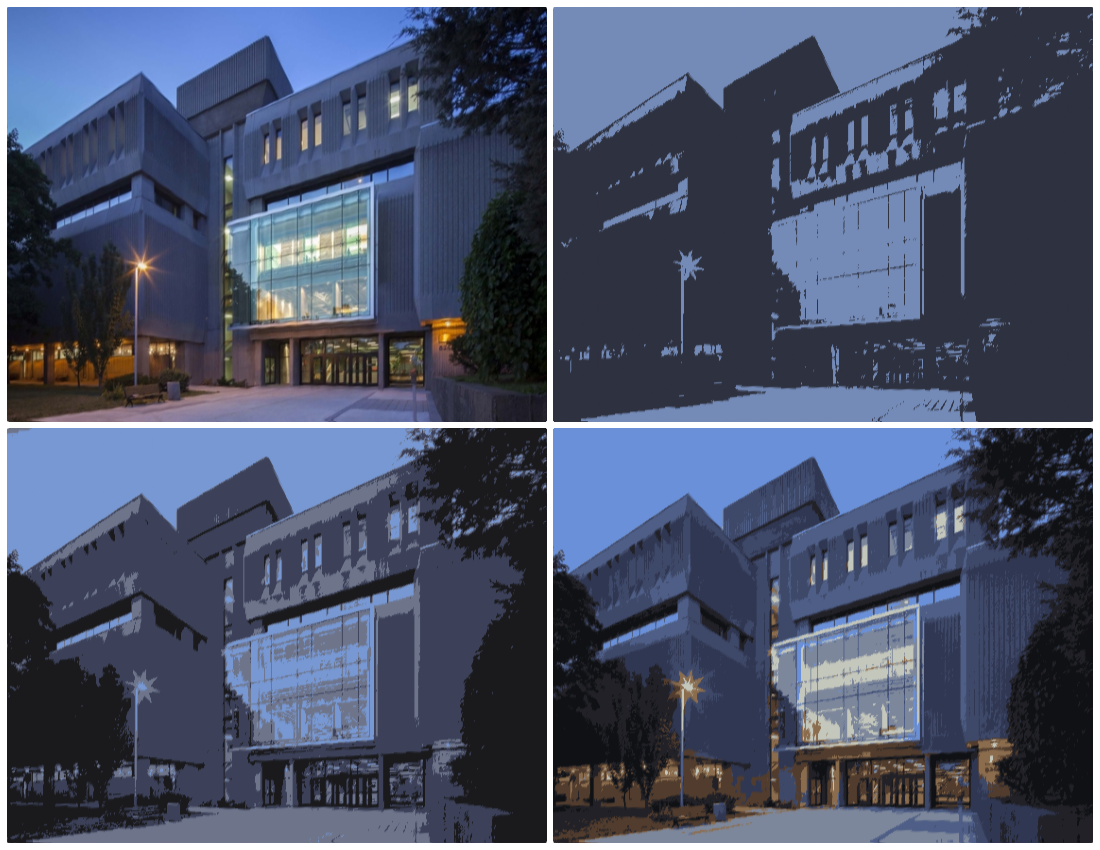
\includegraphics[width=1\textwidth,height=\textheight]{figures/kmoyennes_decelles.png}

}

\caption{\label{fig-decelles}Compression d'image avec l'algorithme des
\(K\)-moyennes: image originale (en haut à gauche), compression avec
trois (en haut à droite), quatre (en bas à gauche) et 10 (en bas à
droite) couleurs.}

\end{figure}%

\section{Mesures de dissemblance}\label{mesures-de-dissemblance}

Comment mesurer si deux observations appartiennent à un même
regroupement et sont similaires? Idéalement, on aimerait avoir une
situation comme dans la Figure~\ref{fig-regroupements-bidons} où les
regroupements sont clairement visibles. On aimerait que la similarité
entre observations d'un même groupe, ou intra-groupe, soit élevée et que
la similarité entre groupe soit faible. Les regroupements devraient être
éloignés les uns des autres, tandis que les observations au sein de ces
regroupements devraient être proches. Dans la plupart des cas, il y aura
des observations isolées qui n'appartiennent pas nécessairement
logiquement à l'un ou l'autre des groupes: on appelle parfois ces
observations aberrances.

\begin{figure}[ht!]

\centering{

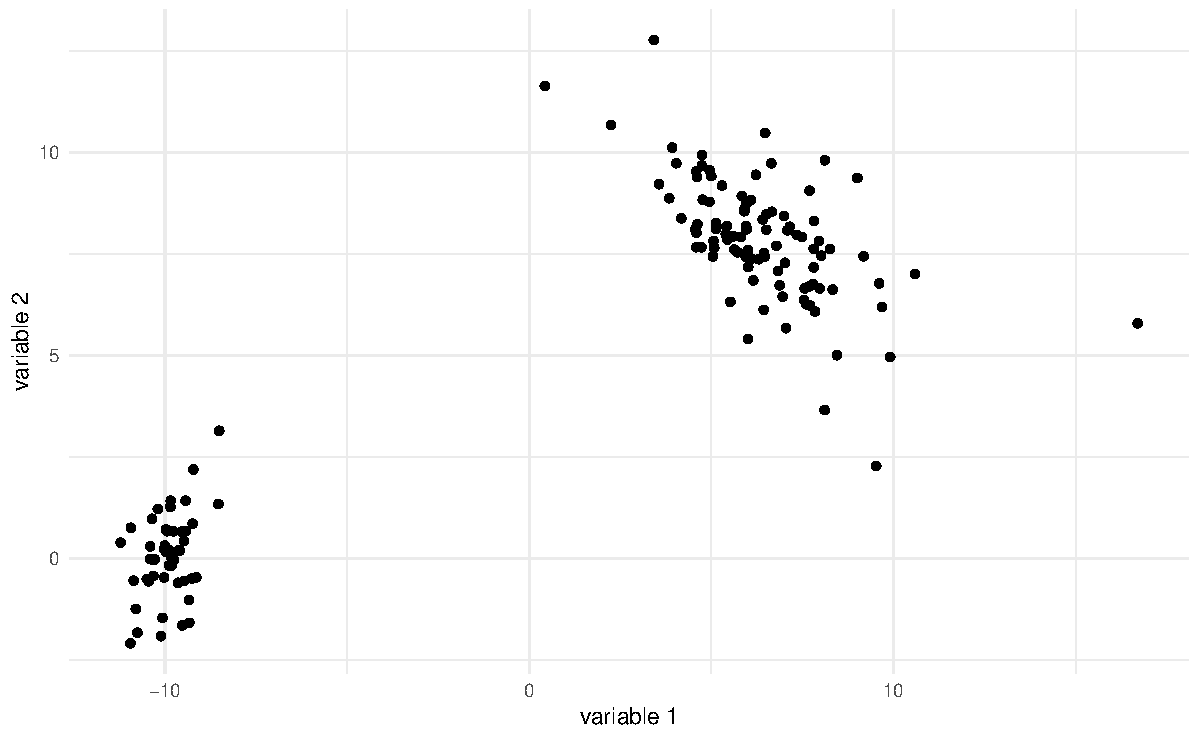
\includegraphics[width=0.85\textwidth,height=\textheight]{regroupements_files/figure-pdf/fig-regroupements-bidons-1.pdf}

}

\caption{\label{fig-regroupements-bidons}Données simulées avec deux
regroupements hypothétiques.}

\end{figure}%

\subsection{Mesures de dissemblance}\label{mesures-de-dissemblance-1}

Les algorithmes de segmentation comparent les observations entre elles:
souvent, la matrice de données est réduite à une mesure de distance
entre observations (soit les lignes de la base de données). Une
\textbf{mesure de dissemblance} sert à quantifier la proximité de deux
objets à partir de leurs coordoonnées. Elle mesure la distance entre
deux vecteurs lignes d'observations \(\mathbf{X}_i\) et \(\mathbf{X}_j\)
en se basant sur les \(p\) variables explicatives. Plus la dissemblance
est petite, plus les sujets \(\mathbf{X}_i\) et \(\mathbf{X}_j\) sont
similaires. La plupart des mesures de dissemblances \(d\) ont les
propriétés mathématiques suivantes:

\begin{enumerate}
\def\labelenumi{\arabic{enumi})}
\tightlist
\item
  \(d(\mathbf{X}_i, \mathbf{X}_j) \geq 0\) (positivité), avec égalité
  (distance nulle) si et seulement si \(\mathbf{X}_i=\mathbf{X}_j\)
  (mêmes caractéristiques pour toutes les variables explicatives);
\item
  \(d(\mathbf{X}_i, \mathbf{X}_j)=d(\mathbf{X}_j, \mathbf{X}_i)\)
  (symmétrie);
\end{enumerate}

Toute mesure de distance\footnote{Une fonction de distance respecte en
  plus l'inégalité du triangle.} est une mesure de dissemblance. La
mesure de dissemblance la plus utilisée en pratique est la distance
euclidienne entre sujets, soit \begin{align*}
d(\mathbf{X}_i, \mathbf{X}_j; l_2) = \left\{(X_{i1}-X_{j1})^2 + \cdots + (X_{ip}-X_{jp})^2\right\}^{1/2}.
\end{align*} C'est tout simplement la longueurdu segment qui relie deux
points dans l'espace \(p\) dimensionnel.

Plus généralement, la distance de Minkowski ou distance \(l_q\) entre
les vecteurs ligne \(\mathbf{X}_i\) et \(\mathbf{X}_j\) est
\begin{align*}
d(\mathbf{X}_i, \mathbf{X}_j; l_q) = \left( \sum_{k=1}^p |X_{ik}-X_{jk}|^q \right)^{1/q},\qquad q > 0;
\end{align*} la distance Euclidienne correspondant à \(q=2\), et la
distance de Manhattan à \(q=1\).\footnote{La distance de Manhattan est
  la somme des valeurs absolues entre chaque composante. En deux
  dimensions, si on considère une ville comme New York dont les rues
  sont quadrillées, cela revient à marcher le long des rues alors que la
  distance Euclidienne traverse les édifices.} Finalement, si
\(q=\infty\), la distance se réduit à \(\max_{k=1}^p |X_{ik}-X_{jk}|\),
soit le maximum des différences entre coordonnées des vecteurs
d'observations.

Il existe un très grand nombre d'autres mesures de dissemblance pour
variables quantitatives, ordinales, nominales et binaires. Si les
variables sont toutes binaires, la mesure d'appariement simple
(\emph{simple matching}), qui mesure la proportion des variables pour
lesquelles les deux sujets ont des valeurs différentes, est une mesure
de dissemblance adéquate.

Dans le cas de jeux de données avec des variables mixes, une option
populaire est la distance de Gower (\citeproc{ref-Gower:1971}{Gower
1971}). Cette dernière compare deux individus selon leurs
caractéristiques et est construite à partir de similarité, avec
\(\mathbf{D} = (\mathbf{I}_n-\mathbf{S})^{1/2}\) comme matrice de
dissimilarité des \(n\) observations. La similarité entre deux individus
est définie comme \begin{align*}
S_{ij} = \frac{\sum_{k=1}^p s_{ijk} \delta_{ijk}}{\sum_{k=1}^p \delta_{ijk}}
\end{align*} où \(\delta_{ijk}\) est un poids qui vaut zéro si la
variable \(\mathrm{X}_k\) est manquante pour l'un ou l'autre des
individus.

On distingue trois type de variables dans la distance de Gowers:

\begin{itemize}
\tightlist
\item
  les variables binaires asymmétrique de type absence/présence donnent
  une valeur de \(\delta=1, s=1\) si les deux sont présentes
  \(X_{ik}=X_{jk}=1\), \(\delta_{ijk}=1\) et \(s_{ijk}=0\) si
  \(X_{ik} \neq X_{jk}\) et \(\delta_{ijk}=0\) si \(X_{ik}=X_{jk}=0\).
\item
  \(s_{ijk}=1\) les variables qualitatives ont la même modalité et
  \(s_{ijk}=0\) sinon
\item
  \(s_{ijk} = 1-|X_{ik}-X_{jk}|/R_k\) pour une variable continue, où
  \(R_k\) est l'étendue de la variable
  \(R_k=\max_{i} X_{ik} - \min_i X_{ik}\) dans l'échantillon.
\end{itemize}

La dissemblance résultante pour les types mixtes vaut zéro quand toutes
les variables sont similaires/égales et un si elles sont complètement
différentes/maximalement distantes.

On peut traiter les variables ordinales soit comme des variables
continues, soit comme des variables nominales avec la mesure
d'appariement simple; ce faisant, on n'utilise pas l'ordre entre les
modalités.

\subsection{Dissemblance et valeurs
manquantes}\label{dissemblance-et-valeurs-manquantes}

Dans plusieurs cas, on se trouvera en présence de valeurs manquantes
dans le jeu de données. Cela peut arriver pour plusieurs raisons
valables (aucune candidature ne représente un partir dans une
circonscription donnée pour un parti lors d'une élection, l'information
est manquante, une femme ne peut avoir de cancer de la prostate, etc.)
Il faut bien penser à vérifier si l'algorithme de votre choix peut gérer
ces valeurs manquantes. Sinon, ces dernières devront être imputées
préalablement à l'analyse de regroupements ou vous devrez faire sans les
variables explicatives correspondantes.

Les définitions des distances révèlent que chaque variable explicative a
le même poids. En revanche, plus une variable a une grande variance,
plus elle aura de l'influence sur le calcul de la distance, ce qui peut
être bon ou mauvais selon la structure des groupes. Règle générale, il
est préférable d'éviter qu'une variable domine dans la segmentation. La
standardisation des variables et les transformations préalables
effectuées sur les variables (log, arcsin, etc.) impacteront le
résultat.

On peut standardiser au préalable les variables avant de faire
l'analyse. Par défaut, les variables continues seront centrées et
réduites, ou standardisées, afin d'avoir une moyenne de zéro et une
variance de un (\texttt{scale}). On peut ensuite faire les analyses
comme précédemment. Si on a des valeurs aberrantes, cela peut impacter
le calcul des moyennes et variances; d'autres estimateurs de
localisation et d'échelles plus robustes, par exemple la médiane et la
déviation absolue par rapport à la médiane (\texttt{mad}) peuvent alors
être plus adéquats pour diminuer l'impact des valeurs aberrantes même si
le coût de calcul associé est plus conséquent. Notez qu'il est illogique
de standardiser les variables binaires et catégorielles.

\begin{Shaded}
\begin{Highlighting}[]
\CommentTok{\# Standardisation usuelle }
\CommentTok{\# (soustraire moyenne, diviser par écart{-}type)}
\NormalTok{donsmult\_std }\OtherTok{\textless{}{-}} \FunctionTok{scale}\NormalTok{(donsmult)}
\CommentTok{\# Standardisation robuste}
\NormalTok{donsmult\_std\_rob }\OtherTok{\textless{}{-}} \FunctionTok{apply}\NormalTok{(}
\NormalTok{  donsmult, }
  \AttributeTok{MARGIN =} \DecValTok{2}\NormalTok{, }
  \AttributeTok{FUN =} \ControlFlowTok{function}\NormalTok{(x)\{(x }\SpecialCharTok{{-}} \FunctionTok{median}\NormalTok{(x))}\SpecialCharTok{/}\FunctionTok{mad}\NormalTok{(x)\})}
\CommentTok{\# apply permet d\textquotesingle{}appliquer une fonction}
\CommentTok{\# par ligne, colonne ou cellule}
\CommentTok{\# MARGIN = 2 indique colonne }
\CommentTok{\# (on centre chaque colonne tour à tour)}
\CommentTok{\# Déviation absolue par rapport à la médiane}
\CommentTok{\# mad = médiane de |obs {-} mediane|}
\end{Highlighting}
\end{Shaded}

\section{Algorithmes pour la
segmentation}\label{algorithmes-pour-la-segmentation}

L'analyse de regroupements est une branche de l'apprentissage
non-supervisé: contrairement à la classification, il n'existe pas de
vraies étiquettes sur lesquelles se baser pour déterminer la qualité
d'une segmentation. Des critères graphiques et des mesures d'homogénéité
peuvent néanmoins déterminer à quel points les segments créés sont
distincts les uns des autres.

L'analyse de regroupements cherche à créer une division de \(n\)
observations de \(p\) variables en \(k\) regroupements. Il existe un
grand nombre d'algorithmes qui permettent de partitionner les données en
regroupements à partir d'un jeu de données ou d'une matrice de
dissemblance. Les sections suivantes survoleront différents algorithmes
en s'attardant à l'heuristique de l'implémentation, aux différentes
étapes de la procédure, aux hyperparamètres qui influencent le résultat
(par ex., le nombre de groupes, la distance minimale entre
regroupements, la forme des regroupements, les éléments représentatifs)
qui détermine la sortie ainsi que les forces et faiblesses des
algorithmes. À l'ère des mégadonnées, la complexité d'un algorithme de
regroupements, une mesure du nombre d'opérations nécessaires pour
effectuer le calcul, impactera le choix possible: l'algorithme de
regroupements hiérarchiques (agglomératif ou divisif), de même que
l'algorithme de partition autour des médoïdes (PAM) sont à proscrire
dans ces scénarios. Outre l'algorithme, il y a des coûts associés au
calcul de la matrice de dissemblance entre chacune des paires des \(n\)
observations: cette opération nécessite \(\mathrm{O}(n^2p)\) flops pour
le calcul et \(\mathrm{O}(n^2)\) entrées de stockage.\footnote{Soit
  740MB d'espace dans la mémoire vive pour stocker la moitié de la
  matrice de dissemblance 13617 par 13617 (la matrice étant
  symmétrique).} Dans le cas de matrice creuses avec beaucoup de zéros,
le coût de stockage et le coût pour réaliser des opérations matricielle
(décomposition en valeurs propres et vecteurs propres) peut être réduit
à l'aide d'algorithmes dédiés.

Les méthodes de regroupement peuvent être regroupées grossièrement dans
les catégories suivantes:

\begin{enumerate}
\def\labelenumi{\arabic{enumi}.}
\tightlist
\item
  méthodes basées sur les centroïdes et les médoïdes (\(k\)-moyennes,
  \(k\)-médoides PAM, CLARA)
\item
  mélanges de modèles (mélanges Gaussiens, etc.)
\item
  méthodes basées sur la connectivité (regroupements hiérarchiques,
  AGNES et DIANA)
\item
  méthodes basées sur la densité (DBScan)
\end{enumerate}

Dans certaines méthodes paramétriques (catégories 1 à 3), le nombre de
groupes est fixé apriori et est un hyperparamètre du modèle. Les
méthodes nonparamétriques déterminent plutôt ce nombre automatiquement,
mais spécifient un paramètre qui contrôle le degré de lissage.

Nous survolerons uniquement les caractéristiques des principales
méthodes.

\subsection{\texorpdfstring{\(K\)-moyennes}{K-moyennes}}\label{k-moyennes}

L'algorithme des \(K\)-moyennes est un des plus couramment employé en
raison de son faible coût. L'idée est la suivante: on assigne chaque
observation à un de \(K\) regroupements et on calcule la distance entre
cette dernière et un prototype \(\boldsymbol{\mu}_k\) pour le
regroupement \(k\). La fonction objective que l'on cherche à minimiser
est \begin{equation}\phantomsection\label{eq-fobjKmoy}{
\min_{\boldsymbol{\mu}_1, \ldots, \boldsymbol{\mu}_K}\min_{\stackrel{r_{ik} \in \{0, 1\}}{r_{i1} + \cdots + r_{iK}=1}}\underset{\text{distance entre obs. $i$ et le prototype le plus près}}{\sum_{i=1}^n \sum_{k=1}^K r_{ik}d(\mathbf{X}_i,  \boldsymbol{\mu}_{k})}
}\end{equation} où \(r_{ik}=1\) si l'observation \(\mathbf{X}_i\) (soit
la \(i\)e ligne de la base de données) est assignée au groupe \(k\). Si
on utilise la distance Euclidienne carrée, alors la fonction objective
correspond à la somme du carré des erreurs au sein de chaque
regroupement et on cherche à minimiser l'erreur quadratique moyenne. Les
coordonnées optimales \(\widehat{\boldsymbol{\mu}}_k\) pour le prototype
si on connaît les étiquettes de groupes sont celles du barycentre des
\(n_k\) observations du groupe \(k\), soit \begin{align*}
\widehat{\boldsymbol{\mu}}_k = \frac{\sum_{i} r_{ik} \mathbf{X}_i}{n_k}, \quad k = 1, \ldots, K;
\end{align*} d'où l'appelation \(K\)-moyennes. Si on utilise plutôt la
distance de Manhattan (\(l_1\)), alors la solution est la médiane
coordonnée par coordonnées des observations du groupe. Il n'est pas
possible de déterminer l'allocation optimale de \(n\) observations en
\(K\) groupes (problème NP complet), mais il est en revanche possible de
trouver rapidement une solution approximative au problème.

Pour ce faire, on sélectionne préalablement un nombre \(K\) de
regroupements et les coordonnées de départ pour les prototypes.
L'algorithme itère entre deux étapes:

\begin{enumerate}
\def\labelenumi{\arabic{enumi}.}
\tightlist
\item
  \textbf{Assignation} (étape E): calculer la distance entre chaque
  observation et les prototypes; assigner chaque observation au
  prototype le plus près.
\item
  \textbf{Mise à jour} (étape M): estimer les coordoonnées des nouveaux
  prototypes; si on utilise la distance Euclidienne, cela revient à
  calculer le barycentre (la moyenne variable par variable) des
  observations assignées aux regroupements.
\end{enumerate}

En pratique, l'algorithme convergera rapidement vers une solution
locale. Cette dernière est simplement une assignation pour laquelle,
d'une itération à l'autre, aucune observation ne change de groupe.

L'algorithme des \(K\)-moyennes présenté offre une forme de
partitionnement dite rigide: chaque observation est assignée à un seul
regroupement. Si cette appartenance unique peut être logique pour les
points à proximité du barycentre, ceux situés à l'intersection des
frontières qui définissent les différents regroupements pourraient
parfois légitimement faire partie d'un ou l'autre de ces derniers. On
pourrait plutôt assigner un poids représentant la probabilité d'être
dans un des \(K\) regroupements, appelé responsabilité et dénotée
\(r_{ik}\). Avec une assignation rigide, \(r_{ik}=1\) si l'observation
\(i\) est dans le regroupement \(k\) et \(r_{ik}=0\) sinon.

Quelquefois, on peut vouloir prédire les étiquettes de groupes de
nouvelles observations. Sans réentraîner l'algorithme, on pourrait ainsi
assigner de nouvelles observations au barycentre le plus près.

Voici quelques forces et faiblesses de la méthode des \(K\)-moyennes

\begin{itemize}
\tightlist
\item
  L'algorithme des \(K\)-moyennes a une complexité \textbf{linéaire}
  dans la dimension et dans le nombre de variables, soit
  \(\mathsf{O}(np)\). Ce faible coût de calcul est un avantage avec des
  mégadonnées (\(n\) grand) et en haute dimension \(p\) grand).
\item
  L'algorithme converge rapidement vers une solution et on a des
  garanties que la solution est un maximum local, puisque l'algorithme
  minimise les répartitions et les prototypes tour à tour.
\item
  Les \(K\)-moyennes créent des regroupements globulaires d'apparence
  sphérique si on utilise la distance Euclidienne: cela revient à faire
  une séparation linéaire de l'espace (voir
  Figure~\ref{fig-voronoikmoy}).
\item
  Chaque observation est assignée à un seul des \(K\) regroupements
  (assignation rigide).
\item
  Comme toutes les observations font partie des \(K\) groupes, les
  valeurs aberrantes ne sont pas traitées à part. Or, la présence de
  valeurs aberrantes impacte le barycentre des observations du groupe.
  Comme ce dernier donne le prototype du groupe, l'algorithme manque de
  robustesse.
\item
  L'algorithme est sensible aux valeurs initiales des prototypes et
  retourne des solutions différentes selon ces dernières.
\end{itemize}

\begin{figure}[ht!]

{\centering 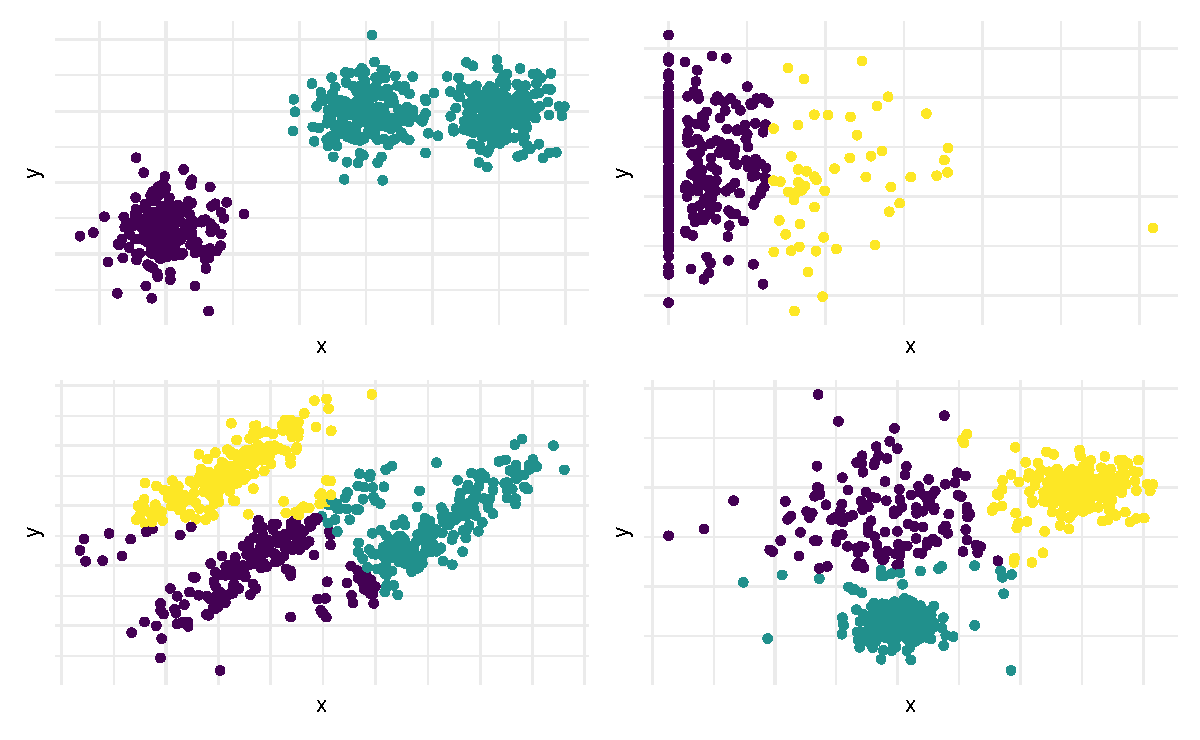
\includegraphics[width=0.85\textwidth,height=\textheight]{regroupements_files/figure-pdf/kmoyperfo-1.pdf}

}

\caption{Performance de l'algorithme des \(K\)-moyennes en fonction de
différents scénarios: (haut, à gauche) nombre incorrect de classe et
données normales de même variance, bien séparées, (haut, à droite)
données avec excès de zéro, un cas où les \(K\)-moyennes ignorent la
topologie des regroupements, et ne segmente pas adéquatement les
regroupements connectés (bas, à gauche) données elliptiques de même
variance, mais fortement corrélées. Comme le critère minimise la
distance intra-groupe sans pondération, les points regroupés
appartiennent à différentes classes et (bas, à droite) données
sphériques de variances différentes. L'algorithme des \(K\)-moyennes
réussit une bonne segmentation si les groupements sont compacts et bien
séparés.}

\end{figure}%

\subsubsection*{Choix des
hyperparamètres}\label{choix-des-hyperparamuxe8tres}
\addcontentsline{toc}{subsubsection}{Choix des hyperparamètres}

L'algorithme des \(K\)-moyennes comporte plusieurs paramètres, dit
hyperparamètres, qui sont fixés par l'utilisateurs préalablement à la
segmentation. Ces derniers incluent

\begin{enumerate}
\def\labelenumi{\arabic{enumi}.}
\tightlist
\item
  les valeurs initiales des prototypes
\item
  le nombre de groupes \(K\)
\item
  le choix de la mesure de distance.
\end{enumerate}

\subsubsection*{Valeurs initiales des
prototypes}\label{valeurs-initiales-des-prototypes}
\addcontentsline{toc}{subsubsection}{Valeurs initiales des prototypes}

Comme mentionné précédemment, les regroupements obtenus peuvent varier
fortement en fonction des valeurs de départ: la
Figure~\ref{fig-kmoyenne-mauvais} montre trois regroupements visibles
avec une segmentation qui fusionne deux groupes apparents (gauche), et
une solution plus sensée à droite. Une segmentation sera supérieure à
une autre si elle a une plus petite valeur de la fonction objective de
l'Équation~\ref{eq-fobjKmoy}: les points seront moins dispersés autour
de leurs prototypes.

\begin{figure}[ht!]

\centering{

\includegraphics[width=0.85\textwidth,height=\textheight]{regroupements_files/figure-pdf/fig-kmoyenne-mauvais-1.pdf}

}

\caption{\label{fig-kmoyenne-mauvais}Résultat d'une analyse de
regroupement avec \(K=3\) groupes avec une mauvaise initialisation
principale (gauche) et une bonne initialisation (droite).}

\end{figure}%

La solution la plus simple est de choisir aléatoirement des coordonnées
initiales pour les prototypes et de répéter la segmentation plusieurs
fois, en choisissant à la fin celle qui a la plus petite valeur du
critère objectif.

On peut également choisir des valeurs suffisamment éloignées:
l'algorithme des \(K\)-moyennes\({}^{++}\) est une variante
algorithmique qui propose de choisir des barycentres éloignés les uns
des autres (ce qui réduit typiquement le nombre d'itérations). Cette
méthode d'initialisation sélectionne une observation au hasard et on
l'assigne comme premier prototype, disons \(\boldsymbol{\mu}_1\). Par la
suite, on procède avec \(k=2, \ldots, K\) aux étapes suivantes:

\begin{enumerate}
\def\labelenumi{\arabic{enumi}.}
\tightlist
\item
  calcul de la distance carrée minimale entre l'observation
  \(\mathbf{X}_i\) et les prototypes précédemment choisis,
  \begin{align*}
  p_i = \min \{d(\mathbf{X}_i, \boldsymbol{\mu}_1; l_2)^2, \ldots, d(\mathbf{X}_i, \boldsymbol{\mu}_{k-1}; l_2)^2)\}
  \end{align*}
\item
  Choisir la valeur initiale du \(k^{\text{e}}\) prototype au hasard
  parmi les observations avec une probabilité de \(p_i/\sum_{j} p_j\)
  pour l'observation \(\mathbf{X}_i\).
\end{enumerate}

À la fin, on obtiendra \(K\) valeurs initiales qui serviront à
l'initialisation. Ce faisant, on peut espérer ne pas avoir à faire
plusieurs allocations aléatoires, puisque les valeurs de départ choisies
sont raisonnablement éloignées les unes des autres.

\subsubsection*{Nombre de regroupements}\label{nombre-de-regroupements}
\addcontentsline{toc}{subsubsection}{Nombre de regroupements}

L'autre paramètre crucial des \(K\)-moyennes est le nombre de
regroupements, \(K\). Il est difficile de savoir combien de
regroupements sélectionner apriori, puisque la visualisation en haute
dimension est difficile et on est souvent loin de la situation présentée
dans la Figure~\ref{fig-kmoyenne-mauvais}. On pourrait envisager de
rouler l'algorithme avec plusieurs valeurs de \(K\) et de comparer les
résultats, mais sur quelle base?

La fonction objective de l'Équation~\ref{eq-fobjKmoy} avec la distance
Euclidienne représente la somme du carré des distances (SCD) entres les
observations d'un groupe et leur barycentre, soit la variabilité totale
des observations des \(K\) différents groupes autour de leur barycentre,
\begin{align*}
\mathsf{SCD}_K = \mathsf{SCD}_{1,K} + \cdots + \mathsf{SCD}_{K,K}
\end{align*} où la somme du carré des distances des observations du
groupe \(k\) (pour lesquelles \(r_{.k}=1\)) \begin{align*}
\mathsf{SCD}_{k,K} &= \underset{\mbox{distance $l_2$ entre obs. du groupe $k$ et barycentre $k$}}{\sum_{i=1}^n r_{ik}\|\mathbf{X}_i -  \boldsymbol{\mu}_{k}\|_2}.
\end{align*} La somme des carrés totales correspond à la somme du carré
des distances au barycentre avec un seul regroupement,
\(\mathsf{SCT} = \mathsf{SCD}_{1}\).

La valeur optimale de la somme du carré des distances mesure va
mécaniquement diminuer à mesure que le nombre de regroupements augmente
parce que le modèle aura plus d'opportunités pour réduire la variabilité
intra-groupe, donc \(\mathsf{SCD}_1 > \mathsf{SCD}_2 \cdots\). En
pratique, cela peut ne pas être le cas si le minimum local est
sous-optimal. Si la réduction de la somme du carré des distances est
négligeable, on pourrait penser que la valeur ajoutée d'un groupe
supplémentaire (qui implique plus de paramètres à estimer et plus de
segments à interpréter) est faible.

On peut calculer un coefficient de détermination, qui mesure pourcentage
de variance expliquée, soit \(R^2(K) = 1-\mathsf{SCD}_K/\mathsf{SCT}\).
De la même manière, on s'attend à une diminution du critère et on
pourrait calculer le \(R^2\) semi-partiel
\(R^2_{\mathrm{sp}}(k) = (\mathsf{SCD}_{k-1} - \mathsf{SCD}_{k})/\mathsf{SCT}\)
pour \(k \geq 2\).\footnote{Ces critères servent également pour les
  regroupement hiérarchiques avec le critère de Ward.}

On pourrait aussi tracer un diagramme de la somme du carré des distances
en fonction de \(K\) en ajoutant une pénalité à notre fonction
objective. En effet, avec la distance Euclidienne carrée, il y a une
analogie à faire avec un modèle de régression et on peut légitimement
utiliser un critère d'information pour guider notre choix de \(K\): le
nombre de paramètres est \(Kp\), soit les valeurs des \(p\) coordonnées
des \(K\) barycentres. On utilisera donc un critère d'information de
type BIC.

Il est possible que ces critères donne beaucoup plus de regroupements
que ce que l'analyste est prêt(e) à envisager. Il faut garder en tête
que, davantage qu'un critère mathématique, l'interprétabilité des
regroupements est notre principale critère. Les critères d'information
peuvent retourner trop ou pas assez de groupe: à titre d'exemple, le
panneau de gauche de la Figure~\ref{fig-coudekmoy} montre la somme du
carré des distances pour la Figure~\ref{fig-kmoyenne-mauvais}; on voit
un coude à \(K=2\), mais il y avait visiblement trois regroupements,
dont deux rapprochés.

\begin{figure}[ht!]

\centering{

\includegraphics[width=0.85\textwidth,height=\textheight]{regroupements_files/figure-pdf/fig-coudekmoy-1.pdf}

}

\caption{\label{fig-coudekmoy}Valeur de la fonction objective (somme du
carré des distances) en fonction du nombre de regroupements \(K\).}

\end{figure}%

\subsubsection*{Mesure de distance}\label{mesure-de-distance}
\addcontentsline{toc}{subsubsection}{Mesure de distance}

Toutes les distances \(l_q\) peuvent être utilisées, mais le choix de la
distance Euclidienne carrée est particulièrement commode et
populaire\footnote{La fonction objective s'apparente alors à la somme du
  carré des erreurs, et donc il y a une analogie à faire avec la
  vraisemblance d'un modèle Gaussien en dimension \(p\) de covariance
  sphérique. Cela légitimise l'emploi de critères d'information pour le
  choix du nombre de regroupements.} entraîne une partition linéaire de
l'espace, comme l'illustre la Figure~\ref{fig-voronoikmoy}. La solution
du problème d'optimisation est explicite, ce qui accélère les calculs
(les prototypes correspondent aux barycentres). Sauf indication
contraire, on supposera dans ce qui suit que la distance entre un point
et un prototype est calculée avec la distance Euclidienne au carré.

\begin{figure}[ht!]

\centering{

\includegraphics[width=0.85\textwidth,height=\textheight]{regroupements_files/figure-pdf/fig-voronoikmoy-1.pdf}

}

\caption{\label{fig-voronoikmoy}Partitions de Voronoï pour les
barycentres (cercles) obtenus dans la solution des \(K\)-moyennes. La
ligne de démarcation qui sépare les groupes est linéaire.}

\end{figure}%

\subsubsection{\texorpdfstring{Application en
\textbf{R}}{Application en R}}\label{application-en-r}

Dans \textbf{R}, la fonction \texttt{kmeans} dans le paquet de base
\texttt{stat} permet de faire l'analyse de regroupement. Elle ne prend
pas en charge les valeurs manquantes. La fonction a plusieurs arguments,
dont les coordonnées initiales des prototypes (\texttt{center}; cet
argument peut également être un entier qui dicte le nombre de groupes),
le nombre maximum d'itération de l'algorithme EM (\texttt{iter.max}) et
le nombre de fois qu'on redémarre l'algorithme avec des valeurs
aléatoires (\texttt{nstart}).

On va estimer le modèle en faisant varier le nombre de regroupements
avec pour chaque valeur de \(K\) 10 ensembles de valeurs de départ
aléatoires.

\begin{Shaded}
\begin{Highlighting}[]
\FunctionTok{set.seed}\NormalTok{(}\DecValTok{60602}\NormalTok{)}
\NormalTok{kmoy }\OtherTok{\textless{}{-}} \FunctionTok{list}\NormalTok{()}
\NormalTok{ngmax }\OtherTok{\textless{}{-}} \DecValTok{10}\NormalTok{L}
\ControlFlowTok{for}\NormalTok{(i }\ControlFlowTok{in} \FunctionTok{seq\_len}\NormalTok{(ngmax))\{}
\NormalTok{ kmoy[[i]] }\OtherTok{\textless{}{-}} \FunctionTok{kmeans}\NormalTok{(donsmult\_std,}
                     \AttributeTok{centers =}\NormalTok{ i,}
                     \AttributeTok{nstart =} \DecValTok{10}\NormalTok{)}
\NormalTok{\}}
\end{Highlighting}
\end{Shaded}

Il suffit ensuite de choisir le nombre de regroupements voulus.
Rappelez-vous que le résultat des k-moyennes est aléatoire (parce que
les valeurs initiales des prototypes le sont) et les étiquettes peuvent
être permutées d'une fois à l'autre même si les regroupements sont les
identiques.

À des fins d'illustration, regardons la solution avec \(K=5\)
regroupements. On pourrait également utiliser l'algorithme
\(K\)-moyennes\({}^{++}\) avec \texttt{kcca} du paquet
\texttt{flexclust}. Le code ci-dessous montre le résultat avec la
distance de Manhattan (\(K\)-médianes)

\begin{Shaded}
\begin{Highlighting}[]
\FunctionTok{set.seed}\NormalTok{(}\DecValTok{60602}\NormalTok{)}
\NormalTok{kmed5 }\OtherTok{\textless{}{-}}\NormalTok{ flexclust}\SpecialCharTok{::}\FunctionTok{kcca}\NormalTok{(}
  \AttributeTok{x =}\NormalTok{ donsmult\_std,}
  \AttributeTok{k =} \DecValTok{5}\NormalTok{,}
  \AttributeTok{family =}\NormalTok{ flexclust}\SpecialCharTok{::}\FunctionTok{kccaFamily}\NormalTok{(}\StringTok{"kmedians"}\NormalTok{),}
  \AttributeTok{control =} \FunctionTok{list}\NormalTok{(}\AttributeTok{initcent =} \StringTok{"kmeanspp"}\NormalTok{))}
\CommentTok{\# Vérifier répartition}
\NormalTok{kmed5}\SpecialCharTok{@}\NormalTok{clusinfo}
\CommentTok{\# Coordonnées des K{-}médianes (standardisées)}
\FunctionTok{t}\NormalTok{(}\FunctionTok{t}\NormalTok{(kmed5}\SpecialCharTok{@}\NormalTok{centers)}\SpecialCharTok{*}\NormalTok{dm\_std }\SpecialCharTok{+}\NormalTok{ dm\_moy)}
\CommentTok{\# Étiquettes}
\NormalTok{kmed5}\SpecialCharTok{@}\NormalTok{cluster}
\end{Highlighting}
\end{Shaded}

Il est toujours utile de regarder la taille des regroupements pour voir
si on ne se trouve pas avec des regroupements fortements débalancés.

\begin{Shaded}
\begin{Highlighting}[]
\NormalTok{kmoy5 }\OtherTok{\textless{}{-}}\NormalTok{ kmoy[[}\DecValTok{5}\NormalTok{]]}
\CommentTok{\# Regarder la répartition}
\NormalTok{kmoy5}\SpecialCharTok{$}\NormalTok{size}
\CommentTok{\#\textgreater{} [1]  993   64 3812 4496 4252}
\end{Highlighting}
\end{Shaded}

On peut étudier les coordonnées des prototypes (par exemple, avec
\texttt{kmoy5\$centers}), mais ici les données standardisées ne sont pas
directement interprétables. On procède plutôt au calcul des statistiques
descriptives des profils rapportées dans le
Tableau~\ref{tbl-kmoy5resume}.

\begin{Shaded}
\begin{Highlighting}[]
\NormalTok{donsmult }\SpecialCharTok{|\textgreater{}}
  \FunctionTok{group\_by}\NormalTok{(}\AttributeTok{groupe =}\NormalTok{ kmoy5}\SpecialCharTok{$}\NormalTok{cluster) }\SpecialCharTok{|\textgreater{}}
  \FunctionTok{summarise\_all}\NormalTok{(mean)}
\end{Highlighting}
\end{Shaded}

\begin{longtable}[]{@{}lrrrrr@{}}

\caption{\label{tbl-kmoy5resume}Moyenne des variables explicatives par
segment (segmentation avec \(K\)-moyennes et cinq regroupements).}

\tabularnewline

\toprule\noalign{}
& 1 & 2 & 3 & 4 & 5 \\
\midrule\noalign{}
\endhead
\bottomrule\noalign{}
\endlastfoot
décompte & 993 & 64 & 3812 & 4496 & 4252 \\
mtdons & 13.92 & 445.49 & 24.98 & 15.32 & 12.11 \\
ndons & 2.98 & 11.38 & 13.71 & 4.00 & 4.63 \\
recence & 64.56 & 67.14 & 27.34 & 29.00 & 172.06 \\
anciennete & 219.46 & 255.45 & 252.77 & 83.59 & 247.85 \\
vdonsmax & 22.39 & 1069.30 & 61.19 & 22.53 & 19.23 \\
ddons & 7.49 & 1.92 & 1.65 & 1.60 & 1.87 \\
nrefusconsec & 1.82 & 0.52 & 0.47 & 0.62 & 3.15 \\
snrefus & 3.17 & 0.88 & 1.05 & 4.23 & 2.71 \\
mpromesse & 15.32 & 620.32 & 45.13 & 17.70 & 7.67 \\

\end{longtable}

Les regroupements obtenus sont interprétables:

\begin{itemize}
\tightlist
\item
  Groupe 1: Petits donateurs, faible nombre de dons. N'ont pas donné
  depuis longtemps. Refus fréquents et délai entre dons élevés
\item
  Groupe 2: Grands donateurs fidèles: plus petit groupe. Ces personnes
  ont fait plusieurs dons, leur valeur maximale est élevée. N'ont pas
  donné récemment.
\item
  Groupe 3: Petits donateurs récidivistes. Dons plus élevés que la
  moyenne mais beaucoup de dons de faible valeur et peu fréquents.
\item
  Groupe 4: Petits nouveaux. Moins d'ancienneté, dons fréquents et refus
  fréquents relativement à l'ancienneté.
\item
  Groupe 5: Petits donateurs inactifs. Plutôt anciens, plusieurs refus.
\end{itemize}

On peut représenter graphiquement les regroupements obtenus sur les
premières composantes principales avec les deux mesures de dissemblance.

\begin{figure}[ht!]

\centering{

\includegraphics[width=0.85\textwidth,height=\textheight]{regroupements_files/figure-pdf/fig-acpkmoy5-1.pdf}

}

\caption{\label{fig-acpkmoy5}Nuage de points des deux premières
composantes principales des observations de dons multiples avec les
étiquettes des regroupements obtenus selon la méthode des \(K\)-moyennes
et \(K\)-médianes avec \(K=5\) regroupements.}

\end{figure}%

Avec les \(K\)-médianes, les personnes qui ont fait des dons plus élevés
sont fusionnés avec d'autres personnes qui ont fait des dons moins
élevés et les groupes sont plus de taille comparable. Selon l'objectif
des regroupements, cela peut être avantageux, mais cibler les donateurs
les plus généreux semble plus logique dans le contexte.

On peut étudier l'impact de l'augmentation du nombre de groupes à l'aide
de différents critères. Le premier est la somme des carrés des distances
intra-groupes.

\begin{Shaded}
\begin{Highlighting}[]
\NormalTok{scd }\OtherTok{\textless{}{-}} \FunctionTok{sapply}\NormalTok{(kmoy, }\ControlFlowTok{function}\NormalTok{(x)\{x}\SpecialCharTok{$}\NormalTok{tot.withinss\})}
\CommentTok{\# Graphiques}
\NormalTok{homogene }\OtherTok{\textless{}{-}} \FunctionTok{homogeneite}\NormalTok{(scd)}
\NormalTok{bic\_kmoy }\OtherTok{\textless{}{-}} \FunctionTok{sapply}\NormalTok{(kmoy, BIC)}
\end{Highlighting}
\end{Shaded}

\begin{figure}[ht!]

\centering{

\includegraphics[width=0.85\textwidth,height=\textheight]{regroupements_files/figure-pdf/fig-homogeneite-1.pdf}

}

\caption{\label{fig-homogeneite}Graphiques de l'homogénéité (\(R\) carré
et \(R\) carré semi-partiel).}

\end{figure}%

On peut aussi observer directement la diminution de la somme du carré
des erreurs en incluant une pénalité. Ici, tous les critères pointent
vers un nombre de regroupements plus élevé que 10, mais ce peut être
trop.

\begin{figure}[ht!]

\centering{

\includegraphics[width=0.85\textwidth,height=\textheight]{regroupements_files/figure-pdf/fig-bickmoy-1.pdf}

}

\caption{\label{fig-bickmoy}Coefficient BIC pour les \(K\)-moyennes en
fonction du nombre de regroupements.}

\end{figure}%

\subsection{\texorpdfstring{\(K\)-médoides}{K-médoides}}\label{k-muxe9doides}

L'algorithme des \(K\)-moyennes spécifie que le barycentre des
regroupements est le prototype. On pourrait également choisir pour ce
dernier une des observations du groupe. Cette approche dite des médoïdes
est plus coûteuse en calcul, mais permet d'avoir une observation
réellement observée et est un peu moins sensible aux extrêmes et aux
aberrances, bien que ce fait soit disputé.

L'algorithme de partition autour des médoïdes (PAM) procède comme suit:

\begin{enumerate}
\def\labelenumi{\arabic{enumi}.}
\tightlist
\item
  Initialisation: sélectionner \(K\) des \(n\) observations comme
  médoïdes initiaux.
\item
  Assigner chaque observation au médoïde le plus près.
\item
  Calculer la dissimilarité totale entre chaque médoïde et les
  observations de son groupe.
\item
  Pour chaque médoïde \((k=1, \ldots, K\)): considérer tous les \(n-K\)
  observations à tour de rôle et permuter le médoïde avec l'observation.
  Calculer la distance totale et sélectionner l'observation qui diminue
  le plus la distance totale.
\item
  Répéter les étapes 2 à 4 jusqu'à ce que les médoïdes ne changent plus.
\end{enumerate}

Puisque qu'on considère chaque observation comme candidat à devenir un
médoïde à chaque étape, le coût de calcul est prohibitif.

L'algorithme CLARA, décrit dans Kaufman and Rousseeuw
(\citeproc{ref-Kaufman.Rousseeuw:1990}{1990}), réduit le coût de calcul
et de stockage en utilisant PAM sur de petits sous-échantillons de
taille \(n_S\). On tire au hasard \(n_S\) observations, qu'on regroupe à
l'aide de PAM pour obtenir \(K\) médoïdes. On assigne ensuite les
observations résiduelles au médoïde le plus près et on calcule la
dissimilarité totale: la qualité de la segmentation est calculée en
obtenant la distance moyenne entre les médoïdes et les observations.
CLARA répète la procédure \(S\) fois et retourne la solution parmi les
\(S\) dissimilarité.

La qualité des regroupements est obtenue en utilisant la moyenne des
distances entre les regroupements et leurs médoïdes. On peut également
tracer un graphique des silhouettes: pour chaque observation, on calcule
la moyenne des dissimilarités entre l'observation \(\mathrm{X}_i\) et
celles de chaque regroupement, disons \(a_i\). On calcule de la même
manière la distance moyenne entre \(\mathrm{X}_i\) et chaque autre
regroupement et on retient le minimum de ces distances, \(b_i\).

La valeur de la silhouette est simplement
\(s_i=(b_i-a_i)/\max\{a_i, b_i\}\). Il est possible que la silhouette
\(s_i\) soit négative: cela indique généralement des observations mal
regroupées. De bons regroupements seront obtenus si la silhouette est
élevée: on s'attend, si les groupes sont très éloignées les uns des
autres, à avoir des profils plus uniformes et une silhouette moyenne
plus élevée.

\begin{figure}[ht!]

\centering{

\includegraphics[width=0.85\textwidth,height=\textheight]{regroupements_files/figure-pdf/fig-silhouette-1.pdf}

}

\caption{\label{fig-silhouette}Profil des silhouettes pour deux
regroupements d'un jeu de données: la segmentation de droite est
supérieure parce que les regroupements sont plus homogènes et mieux
équilibrés.}

\end{figure}%

On estime avec nos données de dons multiples les regroupements. Étant
donné la taille conséquente de la base de données, il est préférable
d'utiliser l'algorithme CLARA (\emph{Clustering large applications}).

\begin{Shaded}
\begin{Highlighting}[]
\NormalTok{kmedoide }\OtherTok{\textless{}{-}} \FunctionTok{list}\NormalTok{()}
\FunctionTok{set.seed}\NormalTok{(}\DecValTok{60602}\NormalTok{)}
\ControlFlowTok{for}\NormalTok{(k }\ControlFlowTok{in} \FunctionTok{seq\_len}\NormalTok{(ngmax))\{}
  \CommentTok{\# Algorithme quadratique en sampsize}
\NormalTok{kmedoide[[k]] }\OtherTok{\textless{}{-}}\NormalTok{ cluster}\SpecialCharTok{::}\FunctionTok{clara}\NormalTok{(}\AttributeTok{x =}\NormalTok{ donsmult\_std,}
               \AttributeTok{k =}\NormalTok{ k,}
               \AttributeTok{sampsize =} \DecValTok{500}\NormalTok{,}
               \AttributeTok{metric =} \StringTok{"euclidean"}\NormalTok{, }\CommentTok{\# distance,}
               \CommentTok{\#cluster.only = TRUE, \# ne conserver que étiquettes}
               \AttributeTok{rngR =} \ConstantTok{TRUE}\NormalTok{, }\CommentTok{\# germe aléatoire depuis R}
               \AttributeTok{pamLike =} \ConstantTok{TRUE}\NormalTok{, }\CommentTok{\# même algorithme que PAM}
               \AttributeTok{samples =} \DecValTok{10}\NormalTok{) }\CommentTok{\#nombre de répétitions}
\NormalTok{\}}
\end{Highlighting}
\end{Shaded}

Comme les \(K\)-moyennes, on fera plusieurs essais pour trouver de
bonnes valeurs de départ. On peut tracer le profil des silhouettes
(Figure~\ref{fig-clarasilhouette})

\begin{Shaded}
\begin{Highlighting}[]
\FunctionTok{plot}\NormalTok{(factoextra}\SpecialCharTok{::}\FunctionTok{fviz\_silhouette}\NormalTok{(kmedoide[[}\DecValTok{4}\NormalTok{]]),}
     \AttributeTok{print.summary =} \ConstantTok{FALSE}\NormalTok{)}
\CommentTok{\#\textgreater{}   cluster size ave.sil.width}
\CommentTok{\#\textgreater{} 1       1  146          0.29}
\CommentTok{\#\textgreater{} 2       2  190          0.25}
\CommentTok{\#\textgreater{} 3       3   90          0.33}
\CommentTok{\#\textgreater{} 4       4   74          0.26}
\end{Highlighting}
\end{Shaded}

\begin{figure}[ht!]

\centering{

\includegraphics[width=0.85\textwidth,height=\textheight]{regroupements_files/figure-pdf/fig-clarasilhouette-1.pdf}

}

\caption{\label{fig-clarasilhouette}Silhouettes pour les données de dons
multiples avec l'algorithme CLARA pour \(K=4\) regroupements.}

\end{figure}%

Puisque les prototypes (médoïdes) sont des observations, on peut
simplement extraire leur identifiant. La sortie inclut plusieurs
éléments dont la taille des regroupements, la valeur du critère PAM,
etc.

\begin{Shaded}
\begin{Highlighting}[]
\NormalTok{medoides\_orig }\OtherTok{\textless{}{-}}\NormalTok{ donsmult[kmedoide[[}\DecValTok{4}\NormalTok{]]}\SpecialCharTok{$}\NormalTok{i.med,]}
\NormalTok{medoides\_orig}
\CommentTok{\# Taille des regroupements}
\NormalTok{kmedoide[[}\DecValTok{4}\NormalTok{]]}\SpecialCharTok{$}\NormalTok{clusinfo}
\end{Highlighting}
\end{Shaded}

Voici quelques avantages et inconvénients des \(K\)-médoides.

\begin{itemize}
\tightlist
\item
  les prototypes sont des observations de l'échantillon.
\item
  la fonction objective est moins impactée par les extrêmes.
\item
  le coût de calcul est prohibitif avec des mégadonnées.
\end{itemize}

\subsection{Mélange de modèles}\label{muxe9lange-de-moduxe8les}

L'algorithme des \(K\)-moyennes fait une allocation rigide: chaque
observation est assignée à un seul regroupement, ignorant de ce fait
l'incertitude rattachée à l'étiquetage des observations. Les frontières
de la région, obtenue en calculant l'intersection des courbes sphériques
de regroupement, sont linéaires.

Peut-être plus problématique, la distance Euclidienne non pondérée
impose des regroupements convexes et sphériques de taille semblable: la
qualité des regroupements des \(K\) moyennes est donc mauvaise si les
regroupements ne sont pas sphériques ou globulaires, ou sont de
concentrations inégales.

Une approche plus générale considère que \(X_1, \ldots, X_p\) sont
tirées d'un mélange à \(K\) composantes de lois spécifiées.
Généralement, on choisit une loi normale multidimensionnelle pour le
\(k\)e groupe \(G\) de moyenne \(\boldsymbol{\mu}_k\) et de variance
\(\boldsymbol{\Sigma}_k\).

Si on savait de quelle composante l'observation originait, on pourrait
simplement obtenir les estimation du maximum de vraisemblance pour les
paramètres de moyenne et de variance. Inversement, si on avait les
valeurs des paramètres, on pourrait déterminer de quel composante
l'observation est la plus susceptible de parvenir à l'aide des poids. Le
modèle est estimé à l'aide de l'algorithme d'espérance-maximisation, qui
itère entre l'estimation des probabilités, et celles des autres
composantes. Le paramètres retournés correspondent à un maximum local,
et on peut également obtenir un estimé de la variabilité de ces
paramètres. Ainsi, le mélange de modèle nous donne accès à la fois à
l'incertitude des paramètres et à la probabilité \(\pi_k\) qu'une
observation appartiennent au groupe \(G_k\).

La loi multinormale est caractérisée par une moyenne (qui peut servir de
prototype) et par une matrice de covariance \(\boldsymbol{\Sigma}_k\).
Si on paramétrise cette dernière, on peut obtenir plus de flexiblité
selon que les variances soient différentes d'une variable à l'autre, ou
que les variables soient corrélées. On peut également spécifier que
certains éléments (structure de corrélation, variances) de
\(\boldsymbol{\Sigma}_k\) sont communes à tous les regroupements. En
laissant les paramètres varier, on peut capturer l'effet de
regroupements de tailles et de densité différente au prix de plus de
paramètres et d'un plus petit nombre d'observations pour estimer chacun
d'entre eux.

Si \(p\) est élevé, la structure de covariance non structurée possède
trop de paramètres pour être utile. On limitera ce nombre en choisissant
plutôt une paramétrisation plus parsimonieuse qui impose des contraintes
sur la forme des ellipsoïdes, propres ou communes à tous les groupes.

La matrice de covariance dans \texttt{mclust} est paramétrisée en
fonction de \(\lambda\), qui contrôle le volume, une matrice diagonale
\(\mathbf{A}\) qui contrôle les variances de chaque observation et
\(\mathbf{D}\) une matrice orthogonale qui permet de créer de la
corrélation entre observations. Un index \(k\) spécifie que cette
composante varie d'un regroupement à l'autre.

Les trois lettres de l'identifiant pour volume/forme/orientation
déterminent si cette composante est égale (\texttt{E}), si elle varie
d'un regroupement à l'autre (\texttt{V}) ou si elle est indéterminée
(\texttt{I}). Par exemple, \texttt{EII} spécifie une matrice de
covariance où chaque composante a variance \(\lambda\) et où les
composantes sont indépendantes. Voir
\texttt{mclust.options("emModelNames")} et la documentation dans le
Tableau 3 de Scrucca et al. (\citeproc{ref-mclust5}{2016}).

\begin{figure}[ht!]

\centering{

\includegraphics[width=0.85\textwidth,height=\textheight]{figures/mclust5-parametrization.png}

}

\caption{\label{fig-modeles}Forme des ellipsoïdes pour le mélange de
modèle selon la forme de la structure de covariance. Image extraite de
Scrucca et al. (\citeproc{ref-mclust5}{2016}) (Figure 2) partagée sous
licence \href{https://creativecommons.org/licenses/by/4.0/}{CC BY 4.0}.}

\end{figure}%

Voici quelques avantages et inconvénients des mélanges de modèles
Gaussiens

\begin{itemize}
\tightlist
\item
  cette approche est plus flexible que les \(K\)-moyennes.
\item
  l'ajout d'une composante uniforme permet de gérer les aberrances
  (supporté par \texttt{mclust}).
\item
  l'algorithme EM garantie la convergence à un minimum local (comme pour
  les \(K\)-moyennes)
\item
  on obtient une assignation probabiliste plutôt que rigide, également
  pour la classification
\item
  le coût de calcul est plus élevé que les \(K\)-moyennes
\item
  le nombre de paramètre des matrices de covariance augmente rapidement
  avec la dimension \(p\)
\end{itemize}

\subsubsection{Hyperparamètres}\label{hyperparamuxe8tres}

Pour le mélange de modèle, on doit fixer apriori le nombre de groupes
\(K\), la forme des ellipsoïdes et les valeurs pour l'initialisation.
Les mêmes considérations pratiques qu'avec les \(K\)-moyennes
s'appliquent, bien qu'ici l'utilisation des critères d'information
permette plus légitimement de choisir le nombre de regroupements.

La forme des ellipsoïdes est un compromis entre simplicité
(d'estimation) et nombre de paramètres: un modèle plus flexible sera
plus difficile à estimer et nécessitera plus de temps de calcul et un
plus grand nombre d'échantillon. En petite dimension, il peut être utile
d'effectuer une visualisation préalable pour déterminer quel type de
modèle serait suffisant. Règle générale, il faut aussi considérer le
nombre de paramètres à estimer (qui dépend de \(p\)) et le nombre
d'observations par regroupement. Comme tous les modèles sont estimés
avec la méthode du maximum de vraisemblance, on peut toujours ajuster
tous les types de structures de covariance pour un nombre de
regroupements \(K\) donné et retourner les critères d'information (BIC)
pour sélectionner le meilleur mélange de modèles. La fonction
\texttt{mclustBIC} du paquet \texttt{mclust} permet de calculer ces
modèles et la méthode \texttt{summary} retourne les trois meilleurs
modèles selon le critère d'information.

\subsubsection{\texorpdfstring{Paquet
\texttt{mclust}}{Paquet mclust}}\label{paquet-mclust}

La stratégie de base du paquet \texttt{mclust}
(\citeproc{ref-mclust5}{Scrucca et al. 2016}) est d'ajuster des mélanges
de modèles gaussiens avec plusieurs structures de covariance en faisant
varier le nombre de regroupements. Le modèle sélectionné parmi tous les
candidats est celui qui a la plus petite valeur du critère BIC: ce
dernier dépend de la qualité de l'ajustement et la pénalité prend en
compte le nombre de paramètres de covariance, en plus des moyennes. Il
est possible d'ajouter une composantes pour le bruit, de manière à
éviter que les valeurs aberrantes impactent négativement la
segmentation.

Une fois le modèle obtenu, plusieurs fonctionalités sont disponibles
pour représenter graphiquement les ellipses des modèle pour chaque paire
de variable, les nuages de points des paires de variables avec
différents symboles et couleurs pour les regroupements, etc.

\begin{Shaded}
\begin{Highlighting}[]
\DocumentationTok{\#\# Mélanges de modèles gaussiens}
\FunctionTok{set.seed}\NormalTok{(}\DecValTok{60602}\NormalTok{)}
\FunctionTok{library}\NormalTok{(mclust)}
\NormalTok{mmg }\OtherTok{\textless{}{-}} \FunctionTok{Mclust}\NormalTok{(}\AttributeTok{data =}\NormalTok{ donsmult\_std,}
       \AttributeTok{G =} \DecValTok{1}\SpecialCharTok{:}\DecValTok{10}\NormalTok{,}
       \CommentTok{\# Ajouter composante uniforme}
       \CommentTok{\#  pour bruit (aberrances)}
       \AttributeTok{initialization =} \FunctionTok{list}\NormalTok{(}\AttributeTok{noise =} \ConstantTok{TRUE}\NormalTok{))}
\CommentTok{\# Résumé de la segmentation}
\FunctionTok{summary}\NormalTok{(mmg)}
\end{Highlighting}
\end{Shaded}

On peut obtenir les étiquettes (avec \texttt{0} pour le bruit) avec
\texttt{mmg\$classification}. Le graphique du critère d'information
Bayésien (BIC) montre le négatif: on cherche donc la structure de
covariance et le nombre qui maximise \(-\mathsf{BIC}\).

\begin{Shaded}
\begin{Highlighting}[]
\FunctionTok{plot}\NormalTok{(mmg, }\AttributeTok{what =} \StringTok{"BIC"}\NormalTok{)}
\end{Highlighting}
\end{Shaded}

\begin{figure}[ht!]

\centering{

\includegraphics[width=0.85\textwidth,height=\textheight]{regroupements_files/figure-pdf/fig-mclustbic-1.pdf}

}

\caption{\label{fig-mclustbic}Valeur du négatif du critère d'information
Bayésien pour les mélanges de modèles gaussiens selon le nombre de
regroupements et la structure de covariance.}

\end{figure}%

Avec notre grande base de données, le modèle identifie neuf
regroupements et un volume variable. On peut utiliser des techniques de
réduction de la dimension pour obtenir une représentation graphique.

\begin{Shaded}
\begin{Highlighting}[]
\CommentTok{\# Matrice des nuage de points (paires de variables)}
\CommentTok{\# plot(mmg, what = "classification")}
\CommentTok{\# Réduction de la dimension}
\NormalTok{reduc\_dim\_mmg }\OtherTok{\textless{}{-}}\NormalTok{ mclust}\SpecialCharTok{::}\FunctionTok{MclustDR}\NormalTok{(mmg)}
\FunctionTok{par}\NormalTok{(}\AttributeTok{mfrow =} \FunctionTok{c}\NormalTok{(}\DecValTok{1}\NormalTok{,}\DecValTok{2}\NormalTok{)) }\CommentTok{\# graphiques côte{-}à{-}côte}
\FunctionTok{plot}\NormalTok{(reduc\_dim\_mmg, }\AttributeTok{what =} \StringTok{"contour"}\NormalTok{)}
\CommentTok{\#\textgreater{} Error in parameters$variance$sigma[, , k]: indice hors limites}
\FunctionTok{plot}\NormalTok{(reduc\_dim\_mmg, }\AttributeTok{what =} \StringTok{"scatterplot"}\NormalTok{)}
\end{Highlighting}
\end{Shaded}

\begin{figure}[ht!]

\centering{

\includegraphics[width=0.9\textwidth,height=\textheight]{regroupements_files/figure-pdf/fig-classifreducmclust-1.pdf}

}

\caption{\label{fig-classifreducmclust}Projection des observations,
colorées par regroupement (gauche) et structure des regroupements avec
ellipsoides de confiance (droite).}

\end{figure}%

\subsection{Regroupements
hiérarchiques}\label{regroupements-hiuxe9rarchiques}

Historiquement très utilisés dans les années 70, les méthodes de
regroupement hiérarchique offrent une méthode déterministe de
regroupement à partir d'une matrice de dissimilarité.

L'algorithme pour la procédure agglomérative procède comme suit:

\begin{enumerate}
\def\labelenumi{\arabic{enumi}.}
\tightlist
\item
  Initialisation: chaque observation forme son propre groupe.
\item
  les deux groupes les plus rapprochés sont fusionnés; la distance entre
  le nouveau groupe et les autres regroupements est recalculée.
\item
  on répète l'étape 2 jusqu'à obtenir un seul regroupement.
\end{enumerate}

La procédure divisive procède de la même façon, mais en partant d'un
seul ensemble et en subdivisant ce dernier jusqu'à ce qu'il y ait autant
d'observations que de groupes. Cette dernière est préférable si on veut
isoler de grands regroupements, mais est rarement employée.

Il y a plusieurs façons de calculer la distance entre deux groupes
d'observations. Selon notre définition, nous obtiendrons des
regroupements différents. Les méthodes les plus populaires incluent

\begin{itemize}
\tightlist
\item
  liaison simple (plus proches voisins)
\item
  liaison complète (voisins les plus éloignés)
\item
  liaison moyenne: utilise la moyenne des distances entre toutes les
  paires de sujets (un pour chaque groupe) provenant des deux groupes.
\item
  méthode de Ward: calcul de l'homogénéité globale
\end{itemize}

\begin{figure}[ht!]

\centering{

\includegraphics[width=0.8\textwidth,height=\textheight]{regroupements_files/figure-pdf/fig-distances-1.pdf}

}

\caption{\label{fig-distances}Distances entre regroupements selon la
liaison (simple, complète, barycentre, homogenéité de Ward).}

\end{figure}%

La méthode de Ward n'est pas définie en terme de distance entre
représentants de groupes, mais plutôt en terme de mesure d'homogénéité
au sein des groupes. Supposons qu'à une étape du processus hiérarchique,
nous avons \(M\) groupes et que nous voulons passer à \(M-1\). Pour
chaque groupe \(k\), nous pouvons calculer la somme des carrés des
distances par rapport à la moyenne du groupe, disons
\(\mathsf{SCD}_{k,M}\): plus cette distance est petite, plus le groupe
est compact et homogène. On calcule ensuite l'homogénéité globale en
faisant la somme de l'homogénéité de tous les groupes, soit
\[\mathrm{H}^{(M)} \equiv \mathsf{SCD}_M = \mathsf{SCD}_{1,M} + \cdots + \mathsf{SCD}_{M,M}.\]
La méthode de Ward va regrouper les deux groupes qui feront augmenter le
moins possible l'homogénéité.

En général, les algorithmes de regroupement hiérarchiques stockent une
matrice de dissemblance \(n \times n\), et donc un coût de stockage
quadratique et un coût de calcul \(\Omega(n^2)\) avec
\(\mathrm{O}(n^3)\). Il faut réaliser que ce coût de calcul est
\textbf{prohibitif} en haute dimension. Certains algorithmique efficaces
pour la méthode de liaison simple permettent un temps de calcul
quadratique sans calcul de toutes les distances, à coût
\(\mathrm{O}(n)\). Si la méthode de liaison simple est la moins coûteuse
du lot, elle n'est pas aussi populaire car elle fonctionne bien si
l'écart entre deux regroupements est suffisamment grand. S'il y a du
bruit entre deux regroupements, la qualité des regroupements en sera
affectée. La méthode de liaison complète est moins sensible au bruit et
aux faibles écarts entre regroupements, mais a tendance à casser les
regroupements globulaires. Puisque le critère d'homogénéité de Ward
ressemble à celui des \(K\)-moyennes, la sortie aura tendance à bien
regrouper les amas globulaires.

Généralement, le résultat de la procédure agglomérative avec la méthode
de liaison simple inclura quelques valeurs isolées et un seul grand
regroupement. Une alternative récente
(\citeproc{ref-Gagolewski:2016}{Gagolewski, Bartoszuk, and Cena 2016}),
appelée Genie, modifie la fonction objective de la méthode de liaison
simple en retenant son efficacité de calcul. Plutôt que de simplement
trouver la paire de regroupements à distance minimale, cette fusion
n'est appliquée que si une mesure d'inéquité est inférieur à un seuil
spécifié par l'utilisateur. Si les regroupements sont fortement
inéquitables, la fusion survient entre les regroupements dont un de la
taille minimale courante. L'implémentation \textbf{R}
(\citeproc{ref-Gagolewski:2021}{Gagolewski 2021}) dans le paquet
\texttt{genieclust} est nettement plus rapide que les autres
alternatives et ne nécessite pas de calculer la matrice de
dissimilarité.

On peut comparer les performances des regroupements hiérarchiques selon
la méthode de groupement. La page web de
\href{https://scikit-learn.org/stable/auto_examples/cluster/plot_linkage_comparison.html}{scikit-learn
developers} montre la performance sur des exemples jouets très
artificiels, qui montre que selon la structure des données, l'impact de
la fonction de liaison. Ici, aucun approche hiérarchique ne performe
mieux que les autres dans tous les exemples.

\subsubsection{Sélection des
hyperparamètres}\label{suxe9lection-des-hyperparamuxe8tres}

Outre le choix de la fonction de liaison qui déterminera la distance
entre les regroupements à chaque étape, on devra choisir le nombre de
regroupements.

On peut représenter le modèle à l'aide d'un \textbf{dendrogramme}, un
arbre dont les feuilles indiquent les regroupements à chaque étape
jusqu'à la racine à la dernière étape. La distance entre chaque
embranchement est déterminée par notre critère: cela nous permet de
sélectionner un nombre de regroupements \(K\) après inspection du
dendrogramme et d'extraire la solution en élaguer l'arbre à cette
profondeur.

\begin{figure}[ht!]

\centering{

\includegraphics[width=0.85\textwidth,height=\textheight]{regroupements_files/figure-pdf/fig-dendrogramme-1.pdf}

}

\caption{\label{fig-dendrogramme}Dendrogramme pour l'exemple de
regroupement hiérarchique avec la méthode de Ward et 20 observations.}

\end{figure}%

La hauteur du dendrogramme donne la valeur du critère associé à la
mesure de regroupement: on peut sélectionne le nombre de regroupements
\(K\) en sélectionnant une étape où la qualité de l'ajustement diminue
drastiquement. Pour le critère de Ward qui utilise l'homogénéité, on
peut créer le pourcentage de variance expliquée, \(R^2\) en calculant
\(R^2_{(M)} = 1-\mathrm{H}_{(M)}/\mathrm{H}_{(1)}\), où
\(\mathrm{H}_{(1)}\) est simplement la somme du carré des distances
distances par rapport à la moyenne lorsque toutes les observations sont
dans un même groupe. Le R-carré semi-partiel, qui mesure la perte
d'homogénéité d'une étape à l'autre, renormalisée par
\(\mathrm{H}_{(1)}\), permet également de mesurer la perte d'homogénéité
(relative) en combinant ces deux groupes. On peut faire un graphique de
ces deux critères en fonction du nombre de regroupements et chercher un
point d'inflection (un coude) à partir duquel la perte d'homogénéité est
moindre ou encore le \(R^2\) augmente plus lentement.

La fonction \texttt{stat::hclust} permet de faire des regroupements
agglomératifs (\texttt{agnes}), mais \texttt{fastcluster} propose une
version avec une empreinte mémoire inférieure. Le paquet
\texttt{cluster} offre de son côté l'algorithme divisif
(\texttt{diana}).

Voici quelques particularités des méthodes de regroupement hiérarchique.

\begin{itemize}
\tightlist
\item
  la solution du regroupement hiérarchique est toujours la même
  (déterministe)
\item
  l'assignation d'une observation à un regroupement est finale
\item
  les aberrances ne sont pas traitées et sont souvent assignées dans des
  regroupements à part
\item
  les méthodes d'arborescence sont faciles à expliquer
\item
  le nombre de groupes n'a pas à être spécifié apriori (une seule
  estimation)
\item
  le coût de calcul est prohibitif, avec une complexité quadratique de
  \(\mathrm{O}(n^2)\) pour la méthode de liaison simple et autrement
  \(\mathrm{O}(n^3)\) pour la plupart des autres fonctions de liaison.
\end{itemize}

\section{Conclusion}\label{conclusion}

Le résultat d'une analyse de regroupements est une étiquette pour chaque
observation. Parfois, la méthode d'analyse de regroupement retourne
également un prototype (le barycentre, une observation du groupe ou la
médiane coordonnée par coordonnée) qui permet d'interpréter les
regroupements.

L'analyse de regroupement est une méthode d'apprentissage non-supervisé:
l'objectif est de déduire la structure présente dans un ensemble de
points sans étiquette préalable (contrairement à la classification).
Ainsi, une fois cqu'on a obtenu les étiquettes, on peut comparer les
regroupements entre eux avant d'effectuer le profilage. Est-ce que les
regroupements sont homogènes et que les observations sont près de leur
représentant de groupe? On pourrait calculer les silhouettes et voir si
les groupes sont bien équilibrés, etc. S'il n'existe pas de solution, il
existe des segmentations de moins bonne qualité (parce que difficilement
interprétables, avec des regroupements qui contiennent une poignée
d'observations). Si la segmentation n'est pas satisfaisante, on retourne
à la planche à dessin et on modifie les variables, la méthode ou la
calibration des hyperparamètres jusqu'à ce qu'on soit satisfaits du
résultat.

\begin{tcolorbox}[enhanced jigsaw, bottomrule=.15mm, toptitle=1mm, opacityback=0, title=\textcolor{quarto-callout-note-color}{\faInfo}\hspace{0.5em}{En résumé}, left=2mm, bottomtitle=1mm, colbacktitle=quarto-callout-note-color!10!white, colback=white, breakable, toprule=.15mm, coltitle=black, arc=.35mm, opacitybacktitle=0.6, colframe=quarto-callout-note-color-frame, titlerule=0mm, leftrule=.75mm, rightrule=.15mm]

\begin{itemize}
\tightlist
\item
  L'objectif d'une analyse de regroupement est de mettre en commun des
  observations de telle sorte que les observations d'un même groupe
  soient le plus semblables possible, et que les groupes soient le plus
  différent possible les uns des autres.
\item
  Chaque observation se voit assigner une étiquette de groupe.
\item
  On procède ensuite à une analyse descriptive, segment par segment, à
  l'aide de prototypes.
\item
  L'analyse de regroupement est une méthode d'apprentissage
  non-supervisée: il n'y a pas de véritable séparation.
\item
  La segmentation n'est utile que si elle a une valeur ajoutée.
\item
  Plusieurs choix de l'analyste (mesure de dissemblance, algorithme ou
  méthode de regroupement, choix des hyperparamètres) peuvent donner une
  segmentation différente. L'analyste a une grande marge de manoeuvre.
\item
  Chaque algorithme de segmentation a des avantages et inconvénients.
\item
  L'algorithme des \(K\)-moyennes est le plus employé et son faible coût
  permet son utilisation avec des mégadonnées.
\item
  Aucun algorithme ne performe uniformément mieux, mais certains sont
  plus faciles à employer que d'autres.

  \begin{itemize}
  \tightlist
  \item
    Avec des mégadonnées, la complexité est un facteur important à
    considérer pour le choix de la méthode.
  \item
    La plupart du temps, le choix des hyperparamètres nécessite un peu
    d'essai et erreur.
  \item
    La segmentation peut être médiocre parce que les hyperparamètres
    sont mal choisis.
  \end{itemize}
\item
  Le nombre de groupes peut être guidé par le contexte: les formules et
  indicateurs de qualité servent de balises.
\end{itemize}

\end{tcolorbox}

\bookmarksetup{startatroot}

\chapter{Données manquantes}\label{donnees-manquantes}

Il arrive fréquemment d'avoir des valeurs manquantes dans notre
échantillon. Ces valeurs peuvent être manquantes pour diverses raisons.
Si on prélève nous-mêmes nos données, un répondant peut refuser de
répondre à certaines questions. Si on acquiert nos données d'une source
externe, les valeurs de certaines variables peuvent être manquantes
directement dans le fichier obtenu. Si on ne prend pas en compte le
méchanisme générant les valeurs manquantes, ces dernières peuvent
également biaiser nos analyses. Le but de ce chapitre est de faire un
bref survol de ce sujet.

\section{Principes de base}\label{principes-de-base}

Soit \(X\) une variable pour laquelle des données sont manquantes. Voici
la définition de trois processus de génération de données manquantes.

\begin{enumerate}
\def\labelenumi{\arabic{enumi})}
\tightlist
\item
  Les données manquantes de \(X\) sont dites \textbf{manquantes de façon
  complètement aléatoire} (MCAR, de l'anglais \emph{missing completely
  at random}) si la probabilité que la valeur de \(X\) soit manquante ne
  dépend ni de la valeur de \(X\) (qui n'est pas observée), ni des
  valeurs des autres variables.
\end{enumerate}

Le fait qu'une variable est manquante peut être relié au fait qu'une
autre soit manquante. Des gens peuvent refuser systématiquement de
répondre à deux questions dans un sondage. Dans ce cas, si la
probabilité qu'une personne ne réponde pas ne dépend pas des valeurs de
ces variables (et de toutes les autres), nous sommes encore dans le cas
MCAR. Si par contre, la probabilité que les gens ne répondent pas à une
question sur leur revenu augmente avec la valeur de ce revenu, alors
nous ne sommes plus dans le cas MCAR.

Le cas MCAR peut se présenter par exemple si des questionnaires, ou des
pages ont été égarés ou détruits par inadvertance (effacées du disque
rigide, etc.) Si les questionnaires manquants constituent un
sous-ensemble choisi au hasard de tous les questionnaires, alors le
processus est MCAR. L'hypothèse que les données manquantes sont
complètement aléatoires est en général considérée comme trop
restrictive.

\begin{enumerate}
\def\labelenumi{\arabic{enumi})}
\setcounter{enumi}{1}
\tightlist
\item
  Les données manquantes de \(X\) sont dites \textbf{données manquantes
  de façon aléatoire} (MAR, de l'anglais \emph{missing at random}) si la
  probabilité que la valeur de \(X\) soit manquante ne dépend pas de la
  valeur de \(X\) (qui n'est pas observée) une fois qu'on a contrôlé
  pour les autres variables.
\end{enumerate}

Il est possible par exemple que les femmes refusent plus souvent que les
hommes de répondre à une question, par exemple de donner leur âge (et
donc, le processus n'est pas MCAR). Si pour les femmes et les hommes, la
probabilité que \(X\) est manquante ne dépend pas de la valeur de \(X\),
alors le processus est MAR. Les probabilités d'avoir une valeur
manquante sont différentes pour les hommes et les femmes mais cette
probabilité ne dépend pas de la valeur de \(X\) elle-même. L'hypothèse
MAR est donc plus faible que l'hypothèse MCAR.

\begin{enumerate}
\def\labelenumi{\arabic{enumi})}
\setcounter{enumi}{2}
\tightlist
\item
  Les données manquantes de \(X\) sont dites \textbf{manquantes de façon
  non-aléatoire} (MNAR, de l'anglais \emph{missing not at random}) si la
  probabilité que la valeur de \(X\) soit manquante dépend de la valeur
  de \(X\) elle-même.
\end{enumerate}

Par exemple, les gens qui ont un revenu élevé pourraient avoir plus de
réticences à répondre à une question sur leur revenu. Un autre exemple
est si une personne transgenre ne répond pas à la question genre (si on
offre seulement deux choix, homme/femme) et aucune autre question ne se
rattache au genre ou à l'identité sexuelle. La méthode de traitement que
nous allons voir dans ce chapitre, l'imputation multiple, est très
générale et est valide dans le cas MAR (et donc aussi dans le cas MCAR).
Le cas MNAR est beaucoup plus difficile à traiter et ne sera pas
considéré ici.

Il n'est pas possible de tester l'hypothèse que le données sont
manquantes de façon aléatoire ou complètement aléatoire; ce postulat
doit donc être déterminé à partir du contexte et des variables
auxiliaires disponibles.

\section{Méthodes d'imputation}\label{muxe9thodes-dimputation}

Il est important de noter que, dans bien des cas, les données manquantes
ont une valeur logique: un client qui n'a pas de carte de crédit a un
solde de 0! Tous ces cas devraient être traités en amon, d'où
l'importance des validations d'usage et du nettoyage préliminaire de la
base de données.

\subsection{Cas complets}\label{cas-complets}

La première idée naïve pour une analyse est de retirer les observations
avec données manquantes pour conserver les cas complets (\emph{listwise
deletion}, ou \emph{complete case analysis}).

Cette méthode consiste à garder seulement les observations qui n'ont
aucune valeur manquante pour les variables utilisées dans l'analyse
demandée. Dès qu'une variable est manquante, on enlève le sujet au
complet. C'est la méthode utilisée par défaut dans la plupart des
logiciels, dont \textbf{R}.

\begin{itemize}
\tightlist
\item
  Si le processus est MCAR, cette méthode est valide car l'échantillon
  utilisé est vraiment un sous-échantillon aléatoire de l'échantillon
  original. Par contre, ce n'est pas nécessairement la meilleure
  solution car on perd de la précision en utilisant moins
  d'observations.
\item
  Si le processus est seulement MAR ou MNAR, cette méthode produit
  généralement des estimations biaisées des paramètres.
\end{itemize}

En général, l'approche des cas complet est la première étape d'une
analyse afin d'obtenir des estimés initiaux que nous corrigerons pas
d'autre méthode. Elle n'est vraiment utile que si la proportion
d'observations manquantes est très faible et le processus est MCAR.
Évidemment, la présence de valeurs manquantes mène à une diminution de
la précision des estimateurs (caractérisée par une augmentation des
erreurs-types) et à une plus faible puissance pour les tests d'hypothèse
et donc ignorer l'information partielle (si seulement certaines valeurs
des variables explicatives sont manquantes) est sous-optimal.

\subsection{Imputation simple}\label{imputation-simple}

L'\textbf{imputation} consiste à remplacer les valeurs manquantes pour
boucher le trous. Pour paraphraser Dempster et Rubin (1983),

\begin{quote}
Le concept d'imputation est à la fois séduisant et dangereux.
\end{quote}

Avec l'\textbf{imputation simple}, on remplace les valeurs manquantes
par des ersatz raisonnables. Par exemple, on peut remplacer les valeurs
manquantes d'une variable par la moyenne de cette variable dans notre
échantillon. On peut aussi ajuster un modèle de régression avec cette
variable comme variable dépendante et d'autres variables explicatives
comme variables indépendantes et utiliser les valeurs prédites comme
remplacement. Une fois que les valeurs manquantes ont été remplacées, on
fait l'analyse avec toutes les observations.

L'imputation par le mode ou la moyenne n'est pas recommandée parce
qu'elle dilue la corrélation entre les variables explicatives et elle
réduit la variabilité. Les modèles de régression mènent également à
une-sous estimation de l'incertitude en raison cette fois-ci de
l'augmentation de la corrélation, ce qui augmente mécaniquement la
significativité des tests, contrairement à l'imputation aléatoire
(droite). Le Figure~\ref{fig-imputation} montre clairement cet état de
fait.

\begin{figure}[ht!]

\centering{

\includegraphics[width=1\textwidth,height=\textheight]{donneesmanquantes_files/figure-pdf/fig-imputation-1.pdf}

}

\caption{\label{fig-imputation}Différences entre méthodes d'imputation,
avec imputation par la moyenne, par le biais d'une régression linéaire
et par un modèle aléatoire de régression, de gauche à droite.}

\end{figure}%

En quoi constitue l'imputation aléatoire recommandée ci-dessus?
Considérons le cas d'une régression logistique pour une variable
explicative binaire. Plutôt que d'assigner à la classe la plus probable,
une prédiction aléatoire simule une variable 0/1 avec probabilité
\((1-\widehat{p}_i, \widehat{p}_i)\). Pour un modèle de régression
linéaire par moindres carrés ordinaires avec vecteur ligne de
prédicteurs \(\mathbf{x}_i\) et matrice de modèle \(\mathbf{X}\), la
prédiction sera tirée de la loi prédictive normale\footnote{Spécifiquement,
  une loi normale avec moyenne
  \(\widehat{y}_i=\mathbf{x}_i\widehat{\boldsymbol{\beta}}\) et variance
  \(\widehat{\sigma}^2\{\mathbf{x}_i\mathbf{X}^\top\mathbf{X})^{-1}\mathbf{x}_i^\top + 1\}\)}.

Il existe d'autres façons d'imputer les valeurs manquantes mais le
problème de toutes ces approches est que l'on ne tient pas compte du
fait que des valeurs ont été remplacées et on fait comme si c'était de
vraies observations. Cela va en général sous-évaluer la variabilité dans
les données. Par conséquent, les écarts-type des paramètres estimés
seront en général sous-estimés et l'inférence (tests et intervalles de
confiance) ne sera pas valide. Cette approche n'est donc \textbf{pas
recommandée}.

Une manière de tenter de reproduire correctement la variabilité dans les
données consiste à ajouter un terme aléatoire dans l'imputation. C'est
ce que fait la méthode suivante, qui possédera l'avantage de corriger
automatiquement les écarts-type des paramètres estimés.

\subsection{Imputation multiple}\label{imputation-multiple}

Cette méthode peut être appliquée dans à peu près n'importe quelle
situation et permet d'ajuster les écarts-type des paramètres estimés.
Elle peut être appliquée lorsque le processus est MAR (et donc aussi
MCAR).

L'idée consiste à procéder à une imputation aléatoire, selon une
certaine technique, pour obtenir un échantillon complet et à ajuster le
modèle d'intérêt avec cet échantillon. On répète ce processus plusieurs
fois et on combine les résultats obtenus.

\begin{center}
\includegraphics[width=0.7\textwidth,height=\textheight]{figures/donnees_manquantes_workflow.pdf}
\end{center}

L'estimation finale des paramètres du modèle est alors simplement la
moyenne des estimations pour les différentes répétitions et on peut
également obtenir une estimation des écarts-type des paramètres qui
tient compte du processus d'imputation.

Plus précisément, supposons qu'on s'intéresse à un seul paramètre
\(\theta\) dans un modèle donné. Ce modèle pourrait être un modèle de
régression linéaire, de régression logistique, etc. Le paramètre
\(\theta\) serait alors un des \(\boldsymbol{\beta}\) du modèle.

Supposons qu'on procède à \(K\) imputations, c'est-à-dire, qu'on
construit \(K\) ensemble de données complets à partir de l'ensemble de
données initial contenant des valeurs manquantes. On estime alors les
paramètres du modèle séparément pour chacun des ensembles de données
imputés. Soit \(\widehat{\theta}_k\), l'estimé du paramètre \(\theta\)
pour l'échantillon \(k \in \{1, \ldots, K\}\) et
\(\widehat{\sigma}_k^2=\mathsf{Va}(\widehat{\theta}_k)\) l'estimé de la
variance de \(\widehat{\theta}_k\) produite par le modèle estimé.

L'estimation finale de \(\theta\), dénotée \(\widehat{\theta}\), est
obtenue tout simplement en faisant la moyenne des estimations de tous
les modèles, c'est-à-dire, \begin{align*}
\widehat{\theta} = \frac{\widehat{\theta}_1 + \cdots + \widehat{\theta}_K}{K}.
\end{align*} Une estimation ajustée de la variance de
\(\widehat{\theta}\) est \begin{align*}
\mathsf{Va}(\hat{\theta}) &= W+ \frac{K+1}{K}B, 
\\ W &= \frac{1}{K} \sum_{k=1}^K \widehat{\sigma}^2_k = \frac{\widehat{\sigma}_1^2 + \cdots + \widehat{\sigma}_K^2}{K},\\
B &= \frac{1}{K-1} \sum_{k=1}^K (\widehat{\theta}_k - \widehat{\theta})^2.
\end{align*} Ainsi, le terme \(W\) est la moyenne des variances et \(B\)
est la variance entre les imputations. Le terme \((1+1/K)B\) est celui
qui vient corriger le fait qu'on travaille avec des données imputées et
non pas des vraies données en augmentant la variance estimée du
paramètre.

C'est ici qu'on voit l'intérêt à procéder à de l'imputation multiple. Si
on procédait à une seule imputation (même en ajoutant une part
d'aléatoire pour essayer de reproduire la variabilité des données), on
ne serait pas en mesure d'estimer la variance inter-groupe de
l'estimateur. Notez que la formule présentée n'est valide que pour le
cas unidimensionnel; l'estimation de la variance dans le cas
multidimensionnel est différente
(\citeproc{ref-Little.Rubin:2019}{Little and Rubin 2019}).

Il faut également ajuster les formules pour le calcul des intervalles de
confiance, valeurs-\(p\) et degrés de liberté. Le logiciel s'en chargera
pour nous.

La méthode d'imputation multiple possède l'avantage d'être applicable
avec n'importe quel modèle sous-jacent. Une fois qu'on a des
échantillons complets (imputés), on ajuste le modèle comme d'habitude.
Mais une observation imputée ne remplacera jamais une vraie observation.
Il faut donc faire tout ce qu'on peut pour limiter le plus possible les
données manquantes.

Il faut utiliser son jugement. Par exemple, si la proportion
d'observations perdues est petite (moins de 5\%), ça ne vaut peut-être
pas la peine de prendre des mesures particulières et on peut faire une
analyse avec les données complètes seulement. S'il y a un doute, on peut
faire une analyse avec les données complètes seulement et une autre avec
imputations multiples afin de valider la première.

Si, à l'inverse, une variable secondaire cause à elle seule une grande
proportion de valeurs manquantes, on peut alors considérer l'éliminer
afin de récupérer des observations. Par exemple, si vous avez une
proportion de 30\% de valeurs manquantes en utilisant toutes vos
variables et que cette proportion baisse à 3\% lorsque vous éliminez
quelques variables peu importantes pour votre étude (ou qui peuvent être
remplacées par d'autres jouant à peu près le même rôle qui elles sont
disponibles), alors vous pourriez considérer la possibilité de les
éliminer. Il est donc nécessaire d'examiner la configuration des valeurs
manquantes avant de faire quoi que ce soit.

Pour l'imputation, nous utiliserons l'algorithme d'imputation multiple
par équations chaînées (MICE).

Avec \(p\) variables \(X_1, \ldots, X_p\), spécifier un ensemble de
modèles \textbf{conditionnels} pour chaque variable \(X_j\) en fonction
de toutes les autres variables, \(\boldsymbol{X}_{-j}\) et les valeurs
observées pour cette variable, \(X_{j, \text{obs}}\).

L'idée est de remplir aléatoire tous les trous et ensuite d'utiliser des
modèles d'imputation aléatoire pour chaque variable à tour de rôle.
Après plusieurs cycles où chacune des variables explicatives (au plus le
nombre de colonnes \(p\)) est imputée, l'impact de l'initialisation
devrait être faible. On retourne alors une copie de la base de données.

\begin{enumerate}
\def\labelenumi{\arabic{enumi}.}
\tightlist
\item
  Initialisation: remplir les trous avec des données au hasard parmi
  \(X_{j, \text{obs}}\) pour \(X_{j, \text{man}}\)
\item
  À l'itération \(t\), pour chaque variable \(j=1, \ldots, p\), à tour
  de rôle:

  \begin{enumerate}
  \def\labelenumii{\alph{enumii})}
  \tightlist
  \item
    tirage aléatoire des paramètres \(\phi_j^{(t)}\) du modèle pour
    \(X_{j,\text{man}}\) conditionnel à \(\boldsymbol{X}_{-j}^{(t-1)}\)
    et \(X_{j, \text{obs}}\)
  \item
    échantillonnage de nouvelles observations \(X^{(t)}_{j,\text{man}}\)
    du modèle avec paramètres \(\phi_j^{(t)}\) conditionnel à
    \(\boldsymbol{X}_{-j}^{(t-1)}\) et \(X_{j, \text{obs}}\)
  \end{enumerate}
\item
  Répéter le cycle
\end{enumerate}

\section{Example d'application de
l'imputation}\label{example-dapplication-de-limputation}

On examine l'exemple de recommandations de l'association professionnelle
des vachers de la section Section~\ref{sec-cowboy}.

Le but est d'examiner les effets des variables \(X_1\) à \(X_6\) sur les
intentions d'achat; la base de données \texttt{manquantes} contient les
observations. Il s'agit des mêmes données que celles du fichier
\texttt{logit1} mais avec des valeurs manquantes.

\begin{longtable}[]{@{}rrrrrrr@{}}

\caption{\label{tbl-missing1r}Tableau de la configuration des données
manquantes.}

\tabularnewline

\toprule\noalign{}
\(X_1\) & \(X_2\) & \(X_3\) & \(X_4\) & \(X_5\) & \(X_6\) & \(y\) \\
\midrule\noalign{}
\endhead
\bottomrule\noalign{}
\endlastfoot
1 & 4 & 0 & 1 & 35 & 2 & 0 \\
. & 1 & 0 & . & 33 & 3 & 0 \\
2 & 3 & 1 & . & 46 & 3 & 0 \\
5 & 2 & 1 & . & 32 & 1 & 1 \\
3 & 2 & 1 & . & 38 & 3 & 1 \\
. & 4 & 0 & 0 & 36 & 3 & 0 \\
. & 3 & 0 & . & 35 & 3 & 0 \\
. & 5 & 1 & 0 & 26 & 2 & 0 \\
. & 3 & 1 & 1 & 39 & 2 & 1 \\
5 & 2 & 1 & . & 38 & 3 & 0 \\

\end{longtable}

Les points (\texttt{.}) indiquent des valeurs manquantes. Le premier
sujet n'a pas de valeur manquante. Le deuxième a une valeur manquante
pour \(X_1\) (emploi) et \(X_4\) (éducation), etc.

Une première façon de voir combien il y a de valeurs manquantes consiste
à faire sortir les statistiques descriptives avec \texttt{summary}.
Ainsi, il y 192 valeurs manquantes pour \(X_1\), 48 pour \(X_2\) et 184
pour \(X_4\). Les autres variables n'ont pas de valeurs manquantes,
incluant la variable dépendante \(Y\). La procédure unidimensionnelle
nous permet seulement de voir combien il y a de valeurs manquantes
variable par variable.

\begin{longtable}[]{@{}llllllll@{}}

\caption{\label{tbl-manquantes-univ}Pourcentage de valeurs manquantes
par variable.}

\tabularnewline

\toprule\noalign{}
& \(X_1\) & \(X_2\) & \(X_3\) & \(X_4\) & \(X_5\) & \(X_6\) & \(y\) \\
\midrule\noalign{}
\endhead
\bottomrule\noalign{}
\endlastfoot
nombre & 192 & 49 & 0 & 184 & 0 & 0 & 0 \\
pourcentage & 0.384 & 0.098 & 0 & 0.368 & 0 & 0 & 0 \\

\end{longtable}

\begin{Shaded}
\begin{Highlighting}[]
\FunctionTok{data}\NormalTok{(manquantes, }\AttributeTok{package =} \StringTok{\textquotesingle{}hecmulti\textquotesingle{}}\NormalTok{)}
\FunctionTok{summary}\NormalTok{(manquantes)}
\CommentTok{\# Pourcentage de valeurs manquantes}
\FunctionTok{apply}\NormalTok{(manquantes, }\DecValTok{2}\NormalTok{, }\ControlFlowTok{function}\NormalTok{(x)\{}\FunctionTok{mean}\NormalTok{(}\FunctionTok{is.na}\NormalTok{(x))\})}
\CommentTok{\# Voir les configurations de valeurs manquantes}
\FunctionTok{md.pattern}\NormalTok{(manquantes)}
\end{Highlighting}
\end{Shaded}

Nous utiliserons le paquet \textbf{R} \texttt{mice} pour faire
l'imputation.

\begin{enumerate}
\def\labelenumi{\arabic{enumi}.}
\tightlist
\item
  Procéder à plusieurs imputations \textbf{aléatoires} pour obtenir un
  échantillon complet (\texttt{mice})
\item
  Ajuster le modèle d'intérêt avec chaque échantillon (\texttt{with}).
  3. Combiner les résultats obtenus (\texttt{pool} et \texttt{summary})
\end{enumerate}

\begin{figure}[ht!]

\centering{

\includegraphics[width=0.7\textwidth,height=\textheight]{donneesmanquantes_files/figure-pdf/fig-manquantes2-1.pdf}

}

\caption{\label{fig-manquantes2}Configurations des valeurs manquantes
pour la base de données \texttt{manquantes}.}

\end{figure}%

La Figure~\ref{fig-manquantes2} donne une indication sur les différentes
combinaisons de données complètes (cases bleues) et les observations
manquantes (cases roses) avec leur fréquence. Les variables sont
indiquées au dessus, le nombre total de valeurs manquantes par variable
en dessous, le nombre d'observations pour chaque configuration de
valeurs manquantes à gauche à gauche et le nombre de variables avec des
valeurs manquantes par configuration à droite. Ainsi, il y a 180 sujets
(36\% de l'échantillon) avec aucune observation manquante. Il y en a 99
avec seulement \(X_4\) manquante et ainsi de suite. On voit donc, par
exemple, que pour 14 sujets, à la fois \(X_1\) et \(X_2\) sont
manquantes.

La recommandation d'usage est d'imputer au moins le pourcentage de cas
incomplet, ici 64\% donc 64 imputations. Si la procédure est trop
coûteuse en calcul, on peut diminuer le nombre d'imputations, mais il
faut au minimum 10 réplications pour avoir une bonne idée de la
variabilité.

On peut comparer l'inférence avec toutes les variables explicatives pour
les données sans valeurs manquantes (\(n=500\) observations), avec les
cas complets uniquement (\(n=180\) observations). Le
Tableau~\ref{tbl-missing3r} présente les estimations des paramètres du
modèle de régression logistique s'il n'y avait pas eu de valeurs
manquantes, avec les cas complets et les résultats de l'imputation
multiple.

Si on ajuste un modèle à une base de données qui contient des valeurs
manquantes, le comportement par défaut est de retirer les observations
qui ont au moins une valeur manquante pour une des variables nécessaires
à l'analyse (voir la sortie de
\texttt{glm(y\ \textasciitilde{}\ .,\ data\ =\ manquantes)}). Il ne
serait pas raisonnable de faire l'analyse avec seulement 180
observations et de laisser tomber les 320 autres. De plus, comme nous
l'avons vu plus haut, ce n'est pas valide à moins que le processus ne
soit MCAR. La partie du milieu du Tableau~\ref{tbl-missing3r} présente
les estimations obtenues. Plusieurs variables significatives à niveau
\(\alpha=0.05\) ne le sont plus (puisqu'il y a moins d'information quand
on réduit le nombre d'observations). Il y a même pire: non seulement la
variable \(\mathsf{I}(X_2=1)\) est passée de significative à non
significative, mais en plus l'estimé de son paramètre a changé de signe.

Nous allons donc faire l'analyse avec l'imputation multiple, en prenant
la méthode d'imputation par défaut

\begin{Shaded}
\begin{Highlighting}[]
\FunctionTok{library}\NormalTok{(mice)}
\CommentTok{\# Imputation multiple avec équations enchaînées}
\CommentTok{\# Intensif en calcul, réduire \textasciigrave{}m\textasciigrave{} si nécessaire}
\NormalTok{impdata }\OtherTok{\textless{}{-}} \FunctionTok{mice}\NormalTok{(}\AttributeTok{data =}\NormalTok{ manquantes,}
                \AttributeTok{m =} \DecValTok{50}\NormalTok{,}
                \AttributeTok{seed =} \DecValTok{2021}\NormalTok{,}
                \AttributeTok{method =} \StringTok{"pmm"}\NormalTok{,}
                \AttributeTok{printFlag =} \ConstantTok{FALSE}\NormalTok{)}
\CommentTok{\# Chaque copie est disponible (1, ..., 50)}
\FunctionTok{complete}\NormalTok{(impdata, }\AttributeTok{action =} \DecValTok{1}\NormalTok{)}
\CommentTok{\# ajuste les modèles avec les données imputées}

\NormalTok{adj\_im }\OtherTok{\textless{}{-}} \FunctionTok{with}\NormalTok{(}\AttributeTok{data =}\NormalTok{ impdata,}
               \AttributeTok{expr =} \FunctionTok{glm}\NormalTok{(y }\SpecialCharTok{\textasciitilde{}}\NormalTok{ x1 }\SpecialCharTok{+}\NormalTok{ x2 }\SpecialCharTok{+}\NormalTok{ x3 }\SpecialCharTok{+}\NormalTok{ x4 }\SpecialCharTok{+}\NormalTok{ x5 }\SpecialCharTok{+}\NormalTok{ x6,}
                          \AttributeTok{family =} \FunctionTok{binomial}\NormalTok{(}\AttributeTok{link =} \StringTok{\textquotesingle{}logit\textquotesingle{}}\NormalTok{)))}

\CommentTok{\# combinaison des résultats }
\NormalTok{fit }\OtherTok{\textless{}{-}} \FunctionTok{pool}\NormalTok{(adj\_im)}
\FunctionTok{summary}\NormalTok{(fit)}
\end{Highlighting}
\end{Shaded}

La procédure \texttt{mice} du paquet éponyme crée les copies complètes
du jeu de données. On peut ensuite appliquer une procédure quelconque et
combiner les estimations avec \texttt{pool}.

\begin{longtable}[t]{lrccrccrcc}

\caption{\label{tbl-missing3r}Estimés, erreurs-type et valeurs-p des
paramètres avec les 500 données complètes (gauche), avec les 180 cas
complets (milieu) et avec l'imputation multiple (droite).}

\tabularnewline

\toprule
\multicolumn{1}{c}{} & \multicolumn{3}{c}{Données complètes} & \multicolumn{3}{c}{Cas complets} & \multicolumn{3}{c}{Imputation multiple} \\
\cmidrule(l{3pt}r{3pt}){2-4} \cmidrule(l{3pt}r{3pt}){5-7} \cmidrule(l{3pt}r{3pt}){8-10}
 & \$\textbackslash{}widehat\{\textbackslash{}boldsymbol\{\textbackslash{}beta\}\}\$ & \$\textbackslash{}mathrm\{se\}(\textbackslash{}widehat\{\textbackslash{}boldsymbol\{\textbackslash{}beta\}\})\$ & valeur-\$p\$ & \$\textbackslash{}widehat\{\textbackslash{}boldsymbol\{\textbackslash{}beta\}\}\$ & \$\textbackslash{}mathrm\{se\}(\textbackslash{}widehat\{\textbackslash{}boldsymbol\{\textbackslash{}beta\}\})\$ & valeur-\$p\$ & \$\textbackslash{}widehat\{\textbackslash{}boldsymbol\{\textbackslash{}beta\}\}\$ & \$\textbackslash{}mathrm\{se\}(\textbackslash{}widehat\{\textbackslash{}boldsymbol\{\textbackslash{}beta\}\})\$ & valeur-\$p\$\\
\midrule
cste & -6.89 & 1.02 & 0.00 & -5.25 & 1.70 & 0.00 & -6.57 & 1.04 & 0.00\\
\$x\_1=1\$ & 0.36 & 0.48 & 0.46 & -0.09 & 0.85 & 0.92 & 0.55 & 0.54 & 0.31\\
\$x\_1=2\$ & -0.47 & 0.37 & 0.21 & -0.57 & 0.66 & 0.39 & -0.13 & 0.45 & 0.78\\
\$x\_1=3\$ & -0.31 & 0.35 & 0.37 & -0.47 & 0.66 & 0.47 & 0.07 & 0.44 & 0.87\\
\$x\_1=4\$ & -0.32 & 0.40 & 0.43 & -0.93 & 0.74 & 0.21 & -0.04 & 0.48 & 0.93\\
\addlinespace
\$x\_2=1\$ & 1.33 & 0.60 & 0.03 & -0.74 & 1.14 & 0.52 & 1.10 & 0.65 & 0.09\\
\$x\_2=2\$ & 1.15 & 0.50 & 0.02 & 0.46 & 0.91 & 0.61 & 1.03 & 0.55 & 0.06\\
\$x\_2=3\$ & 0.77 & 0.48 & 0.11 & -0.41 & 0.89 & 0.64 & 0.52 & 0.52 & 0.31\\
\$x\_2=4\$ & -1.11 & 0.54 & 0.04 & -2.74 & 1.02 & 0.01 & -1.04 & 0.57 & 0.07\\
\$x\_3\$ & 1.35 & 0.26 & 0.00 & 0.80 & 0.44 & 0.07 & 1.19 & 0.27 & 0.00\\
\addlinespace
\$x\_4\$ & 1.83 & 0.30 & 0.00 & 2.25 & 0.58 & 0.00 & 1.52 & 0.37 & 0.00\\
\$x\_5\$ & 0.11 & 0.02 & 0.00 & 0.11 & 0.03 & 0.00 & 0.10 & 0.02 & 0.00\\
\$x\_6=1\$ & 2.41 & 0.38 & 0.00 & 2.23 & 0.66 & 0.00 & 2.26 & 0.38 & 0.00\\
\$x\_6=2\$ & 1.04 & 0.25 & 0.00 & 0.83 & 0.44 & 0.06 & 1.00 & 0.25 & 0.00\\
\bottomrule

\end{longtable}

On peut remarquer que la précision est systématiquement meilleure avec
l'imputation multiple; les erreurs-type pour l'imputation multiple sont
plus petits que celle du modèle qui retire les données incomplètes.

On voit que la variable \(X_3\) (sexe) est significative avec
l'imputation multiple. Son paramètre estimé est 1.19, comparativement à
1.349 s'il n'y avait pas eu de valeurs manquantes. La précision dans
l'estimation avec l'imputation multiple est seulement un peu moins bonne
(erreur-type de 0.27) que celle s'il n'y avait pas eu de manquantes
(erreur type de 0.26). Le paramètre de \(\mathsf{I}(X_6=2)\) redevient
aussi significatif, alors qu'il ne l'était plus si on retirait les
manquantes. Il est peu probable que les données soit \(\mathsf{MCAR}\)
et donc les résultats de l'analyse des cas complets seraient biaisés.

\begin{tcolorbox}[enhanced jigsaw, bottomrule=.15mm, toptitle=1mm, opacityback=0, title=\textcolor{quarto-callout-note-color}{\faInfo}\hspace{0.5em}{En résumé}, left=2mm, bottomtitle=1mm, colbacktitle=quarto-callout-note-color!10!white, colback=white, breakable, toprule=.15mm, coltitle=black, arc=.35mm, opacitybacktitle=0.6, colframe=quarto-callout-note-color-frame, titlerule=0mm, leftrule=.75mm, rightrule=.15mm]

\begin{itemize}
\tightlist
\item
  Les données manquantes réduisent la quantité d'information disponible
  et augmentent l'incertitude.
\item
  On ne peut \textbf{pas} les ignorer (étude des cas complets) sans
  biaiser les interprétations et réduire la quantité d'information
  disponible.
\item
  Pour bien capturer l'incertitude et ne pas modifier les relations
  entre variables, il faut utiliser une méthode d'imputation aléatoire.
\item
  Avec l'algorithme MICE, on utilise un modèle conditionnel pour chaque
  variable à tour de rôle.
\item
  L'imputation multiple est préférée à l'imputation simple car elle
  permet d'estimer l'incertitude sous-jacente en raison des données
  manquantes.
\item
  Il faut un traitement spécial pour les erreurs-type, degrés de
  liberté, valeurs-\(p\) et intervalles de confiance.
\end{itemize}

\end{tcolorbox}

\bookmarksetup{startatroot}

\chapter*{Références}\label{ruxe9fuxe9rences}
\addcontentsline{toc}{chapter}{Références}

\markboth{Références}{Références}

\phantomsection\label{refs}
\begin{CSLReferences}{1}{0}
\bibitem[\citeproctext]{ref-dAstous:2000}
d'Astous, A. 2000. \emph{Le Projet de Recherche En Marketing}. Edited by
Chenelière/McGraw-Hill. 2nd ed.

\bibitem[\citeproctext]{ref-Gagolewski:2021}
Gagolewski, Marek. 2021. {``\texttt{genieclust}: Fast and Robust
Hierarchical Clustering.''} \emph{SoftwareX} 15 (July).
\url{https://doi.org/10.1016/j.softx.2021.100722}.

\bibitem[\citeproctext]{ref-Gagolewski:2016}
Gagolewski, Marek, Maciej Bartoszuk, and Anna Cena. 2016. {``Genie: A
New, Fast, and Outlier-Resistant Hierarchical~Clustering~Algorithm.''}
\emph{Information Sciences} 363: 8--23.
\url{https://doi.org/10.1016/j.ins.2016.05.003}.

\bibitem[\citeproctext]{ref-Gower:1971}
Gower, J. C. 1971. {``A General Coefficient of Similarity and Some of
Its Properties.''} \emph{Biometrics} 27 (4): 857--71.
\url{https://doi.org/10.2307/2528823}.

\bibitem[\citeproctext]{ref-Grambsch.Therneau:1994}
Grambsch, Patricia M., and Terry M. Therneau. 1994. {``{Proportional
hazards tests and diagnostics based on weighted residuals}.''}
\emph{Biometrika} 81 (3): 515--26.
\url{https://doi.org/10.1093/biomet/81.3.515}.

\bibitem[\citeproctext]{ref-Kaufman.Rousseeuw:1990}
Kaufman, Leonard, and Peter J. Rousseeuw. 1990. \emph{Finding Groups in
Data: An Introduction to Cluster Analysis}. Edited by Wiley. Hoboken,
NY. \url{https://doi.org/10.1002/9780470316801}.

\bibitem[\citeproctext]{ref-Little.Rubin:2019}
Little, Roderick J. A., and Donald B Rubin. 2019. {``Statistical
Analysis with Missing Data.''} Edited by Wiley.
\url{https://doi.org/10.1002/9781119482260}.

\bibitem[\citeproctext]{ref-McCullagh:1980}
McCullagh, Peter. 1980. {``Regression Models for Ordinal Data.''}
\emph{Journal of the Royal Statistical Society: Series B
(Methodological)} 42 (2): 109--27.
\url{https://doi.org/10.1111/j.2517-6161.1980.tb01109.x}.

\bibitem[\citeproctext]{ref-mclust5}
Scrucca, Luca, Michael Fop, T. Brendan Murphy, and Adrian E. Raftery.
2016. {``\texttt{mclust} 5: Clustering, Classification and Density
Estimation Using {G}aussian Finite Mixture Models.''} \emph{The R
Journal} 8: 289--317. \url{https://doi.org/10.32614/RJ-2016-021}.

\bibitem[\citeproctext]{ref-Stensrud.Hernan:2020}
Stensrud, Mats J., and Miguel A. Hernán. 2020. {``{Why Test for
Proportional Hazards?}''} \emph{JAMA} 323 (14): 1401--2.
\url{https://doi.org/10.1001/jama.2020.1267}.

\end{CSLReferences}

\bookmarksetup{startatroot}

\chapter{Régression linéaire}\label{regression-lineaire}

Les modèles de régression servent à modéliser la moyenne\footnote{Formellement,
  on parle d'espérance conditionnelle, ou moyenne théorique, en
  supposant que les valeurs des variables explicatives \(\mathbf{X}\)
  sont exogènes, ou connues d'avance: l'inférence est faite
  conditionnellement à ces valeurs.} d'une variable réponse \(Y\) en
fonction de \(p\) variables explicatives (appelées parfois régresseurs
ou covariables) à l'aide d'une équation de la forme \begin{align*}
\underbrace{\mathsf{E}(Y_i \mid \mathbf{X}_i)}_{\text{moyenne de la $i$e réponse}}=\underbrace{\beta_0 + \beta_1\mathrm{X}_{i1} + \cdots + \beta_p \mathrm{X}_{ip}}_{\text{combinaison linéaire de variables explicatives}}.
\end{align*} où \(\mathrm{X}_{ij}\) est la \(i\)e ligne, \(j\)e colonne
du tableau contenant variables explicatives (chaque colonne correspond à
une variable).

Dans le modèle de régression ordinaire, toutes les observations qui ont
les mêmes charactéristiques (c'est-à-dire, les mêmes valeurs des
variables explicatives) ont la même moyenne, même si les observations ne
sont pas identiques.

On peut ajouter un terme d'erreur qui sert à tenir compte du fait
qu'aucune relation linéaire exacte ne lie \(\mathbf{X}\) et \(Y\), ou
que les mesures de \(Y\) contiennent des erreurs. Ce terme d'erreur
aléatoire \(\varepsilon\), souvent supposé tiré d'une loi normale,
servira de base à l'inférence car il permettra de quantifier
l'adéquation entre notre modèle et les données.

On peut réécrire le modèle linéaire en terme de l'erreur pour un
échantillon aléatoire de taille \(n\): dénotons par \(Y_i\) la valeur de
\(Y\) pour le sujet \(i\), et \(\mathrm{X}_{ij}\) la valeur de la \(j\)e
variable explicative du sujet \(i\). Le modèle de régression linéaire
est \begin{equation}\phantomsection\label{eq-olsmean}{
\underbrace{Y_i}_{\text{réponse}} = \underbrace{\beta_0 + \beta_1 \mathrm{X}_{i1} + \ldots + \beta_p \mathrm{X}_{ip}}_{\text{moyenne}} + \underbrace{\varepsilon_{i}}_{\text{erreur}}
}\end{equation} où \(\varepsilon_i\) est le terme d'erreur
\((i=1, \ldots, n\)). Si aucune hypothèse sur la loi aléatoire de
l'erreur n'est spécifiée, on fixe a minima la moyenne théorique du terme
d'erreur à zéro car on postule qu'il n'y a pas d'erreur systématique.

Le postulat de normalité sert à exprimer ce fait et à caractériser les
déviations possibles: on suppose que la probabilité d'observer une
valeur supérieure ou inférieure est la même, mais que les déviations
importantes par rapport à la moyenne sont moins plausibles. Ce postulat
de normalité en est un de convenance: on pénalise les déviations par
rapport à \(\mu\) et l'écart-type commun à toutes les observations,
\(\sigma\), mesure cette écart. S'il y a peu de bruit et que la relation
linéaire entre les variables explicatives et la réponse est très forte
(capturée par la corrélation entre variables), le modèle reflètera
adéquatement les données et l'écart-type estimé sera faible.

La flexibilité du modèle linéaire vient de sa formulation: on spécifie
la moyenne de la réponse \(Y\) comme \textbf{combinaison linéaire de
variables explicatives}, dont le choix est arbitraire. Il est important
de remarquer que ce modèle est linéaire dans les coefficients
\(\boldsymbol{\beta}\in \mathbb{R}_{p+1}\), pas dans les variables
explicatives. Ces dernières sont quelconques et peuvent être des
fonctions (non)-linéaires d'autres variables explicatives, par exemple
\(\mathrm{X}=\log(\texttt{annees})\),
\(\mathrm{X}=\texttt{puissance}^2\) ou
\(\mathrm{X}= \mathsf{I}_{\texttt{homme}}\cdot\mathsf{I}_{\texttt{titulaire}}\).
C'est ce qui fait la flexibilité du modèle linéaire: ce dernier est
principalement employé aux fins suivantes:

\begin{enumerate}
\def\labelenumi{\arabic{enumi}.}
\tightlist
\item
  Comprendre comment et dans quelle mesure les variables explicatives
  \(\mathbf{X}\) influencent la moyenne de la réponse \(Y\)
  (description).
\item
  Quantifier l'influence des variables explicatives \(\mathbf{X}\) sur
  la régressande \(Y\) et tester leur significativité.
\item
  Prédire les valeurs de \(Y\) pour de nouveaux ensembles de covariables
  \(\mathbf{X}\).
\end{enumerate}

\section{Exemple et motivation}\label{exemple-et-motivation}

Le modèle linéaire est sans conteste le modèle statistique le plus
couramment employé. Une grande panoplie de tests statistiques
(tests-\emph{t}, analyse de variance) sont des cas particuliers de
régression linéaire.

Afin de rendre plus tangible le concept et les notions qui touchent aux
modèles linéaires, on présentera ces notions dans le cadre d'un exemple.
On s'intéresse à la discrimination salariale dans un collège américain,
au sein duquel une étude a été réalisée pour investiguer s'il existait
des inégalités salariales entre hommes et femmes. Le jeu de données
\texttt{salaireprof} contient les variables suivantes

\begin{itemize}
\tightlist
\item
  \texttt{salaire}: salaire de professeurs pendant l'année académique
  2008--2009 (en milliers de dollars USD).
\item
  \texttt{echelon}: échelon académique, soit adjoint (\texttt{adjoint}),
  aggrégé (\texttt{aggrege}) ou titulaire (\texttt{titulaire}).
\item
  \texttt{domaine}: variable catégorielle indiquant le champ d'expertise
  du professeur, soit appliqué (\texttt{applique}) ou théorique
  (\texttt{theorique}).
\item
  \texttt{sexe}: indicateur binaire pour le sexe, \texttt{homme} ou
  \texttt{femme}.
\item
  \texttt{service}: nombre d'années de service.
\item
  \texttt{annees}: nombre d'années depuis l'obtention du doctorat.
\end{itemize}

Une analyse exploratoire des données est de mise avant d'ébaucher un
modèle. Si le salaire augmente au fil des ans, on voit que
l'hétérogénéité change en fonction de l'échelon et qu'il y a une
relation claire entre ce dernier et le nombre d'années de service (les
professeurs n'étant éligibles à des promotions qu'après un certain
nombre d'années). Les professeurs adjoints qui ne sont pas promus sont
généralement mis à la porte, aussi il y a moins d'occasions pour que les
salaires varient sur cette échelle.

\begin{figure}[ht!]

\centering{

\includegraphics[width=0.9\textwidth,height=\textheight]{rappel-regressionlineaire_files/figure-pdf/fig-edacollege-1.pdf}

}

\caption{\label{fig-edacollege}Analyse exploratoire des données
\(\texttt{salaireprof}\): répartition des salaires en fonction de
l'échelon et du nombre d'années de service}

\end{figure}%

Ainsi, le salaire augmente avec les années, mais la variabilité croît
également. Il y a peu de femmes dans l'échantillon: moins d'information
signifie moins de puissance pour détecter de petites différences de
salaire. Si on fait un tableau de contingence de l'échelon et du sexe,
on peut calculer la proportion relative homme/femme dans chaque échelon:
16\% des profs adjoints, 16\% pour les aggrégés, mais seulement 7\% des
titulaires alors que ces derniers sont mieux payés en moyenne.

\begin{longtable}[]{@{}lrrr@{}}

\caption{\label{tbl-tableaucontingence}Tableau de contingence donnant le
nombre de professeurs du collège par sexe et par échelon académique.}

\tabularnewline

\toprule\noalign{}
& adjoint & aggrege & titulaire \\
\midrule\noalign{}
\endhead
\bottomrule\noalign{}
\endlastfoot
femme & 11 & 10 & 18 \\
homme & 56 & 54 & 248 \\

\end{longtable}

Le modèle linéaire simple n'inclut qu'une variable explicative et
consiste en une droite d'équation \(y=\beta_0 + \beta_1 \mathrm{X}\) qui
passe à travers un nuage de points. La Figure~\ref{fig-droitenuage}
montre la droite de régression dans le nuage de points formé par les
couples \(\{\mathrm{X}_i, y_i\}\), où \(y_i\) est le \texttt{salaire} et
\(\mathrm{X}\) est \texttt{service}.

\textbf{Programmation}: Pour ajuster un modèle linéaire avec \textbf{R},
on utilise la fonction \texttt{lm}. Le premier argument est une formule,
sous la forme \texttt{y\ \textasciitilde{}\ x} où \texttt{y} est la
variable réponse et \texttt{x} la variable explicative. La fonction
utilisera (si disponible) les variables disponibles dans la base de
données spécifiée via l'argument \texttt{data}. Ici, notre variable
réponse est le \texttt{salaire} et nous tentons d'expliquer ce dernier
en fonction du nombre d'années de service, ici représenté par la
variable continue \texttt{service}.

\begin{Shaded}
\begin{Highlighting}[]
\FunctionTok{data}\NormalTok{(salaireprof, }\AttributeTok{package =} \StringTok{"hecmulti"}\NormalTok{)}
\NormalTok{modlin1 }\OtherTok{\textless{}{-}} \FunctionTok{lm}\NormalTok{(salaire }\SpecialCharTok{\textasciitilde{}}\NormalTok{ service, }\AttributeTok{data =}\NormalTok{ salaireprof)}
\FunctionTok{summary}\NormalTok{(modlin1)}
\CommentTok{\#\textgreater{} }
\CommentTok{\#\textgreater{} Call:}
\CommentTok{\#\textgreater{} lm(formula = salaire \textasciitilde{} service, data = salaireprof)}
\CommentTok{\#\textgreater{} }
\CommentTok{\#\textgreater{} Residuals:}
\CommentTok{\#\textgreater{}    Min     1Q Median     3Q    Max }
\CommentTok{\#\textgreater{} {-}81.93 {-}20.51  {-}3.78  16.42 101.95 }
\CommentTok{\#\textgreater{} }
\CommentTok{\#\textgreater{} Coefficients:}
\CommentTok{\#\textgreater{}             Estimate Std. Error t value        Pr(\textgreater{}|t|)    }
\CommentTok{\#\textgreater{} (Intercept)    99.97       2.42   41.37         \textless{} 2e{-}16 ***}
\CommentTok{\#\textgreater{} service         0.78       0.11    7.06 0.0000000000075 ***}
\CommentTok{\#\textgreater{} {-}{-}{-}}
\CommentTok{\#\textgreater{} Signif. codes:  0 \textquotesingle{}***\textquotesingle{} 0.001 \textquotesingle{}**\textquotesingle{} 0.01 \textquotesingle{}*\textquotesingle{} 0.05 \textquotesingle{}.\textquotesingle{} 0.1 \textquotesingle{} \textquotesingle{} 1}
\CommentTok{\#\textgreater{} }
\CommentTok{\#\textgreater{} Residual standard error: 28.6 on 395 degrees of freedom}
\CommentTok{\#\textgreater{} Multiple R{-}squared:  0.112,  Adjusted R{-}squared:  0.11 }
\CommentTok{\#\textgreater{} F{-}statistic: 49.8 on 1 and 395 DF,  p{-}value: 0.00000000000753}
\end{Highlighting}
\end{Shaded}

Une fois le modèle estimé, on peut extraire les coefficients avec la
méthode \texttt{coef}, ici via \texttt{coef(modlin1)}, ou imprimer un
tableau résumé avec \texttt{summary}. Ce dernier contient quatre
colonnes qui donnent

\begin{itemize}
\tightlist
\item
  les estimations des paramètres de la moyenne \(\widehat{\beta}\)
\item
  les erreur-types des estimations \(\mathsf{se}(\widehat{\beta})\) (qui
  représente leur incertitude)
\item
  la statistique \(t\) obtenue en comparant la valeur de
  \(\widehat{\beta}\) à la valeur sous l'hypothèse nulle \(\beta=0\),
  standardisée par l'erreur-type,
  \(t=\widehat{\beta}/\mathsf{se}(\widehat{\beta})\).
\item
  la valeur-\(p\) pour le test \(\beta_i=0\).
\end{itemize}

Notez qu'on ignore systématiquement les valeurs-\(p\) pour la première
ligne qui correspond à l'ordonnée à l'origine \texttt{(Intercept)}.

\begin{figure}[ht!]

\centering{

\includegraphics[width=0.7\textwidth,height=\textheight]{rappel-regressionlineaire_files/figure-pdf/fig-droitenuage-1.pdf}

}

\caption{\label{fig-droitenuage}Régression linéaire simple pour le
salaire en fonction des années de service; la droite satisfait le
critère des moindres carrés.}

\end{figure}%

Une infinité de droites pourraient passer dans le nuage de points; il
faut donc choisir la meilleure droite (selon un critère donné). Le
critère des moindres carrés, qui consiste à minimiser la somme du carré
des erreurs (soit la somme de la distance verticale entre la droite et
les observations) permet d'obtenir des estimations des paramètres. La
solution du problème d'optimisation est explicite et facilement calculée
par n'importe lequel logiciel.

Les estimateurs des moindres carrés ordinaires
\(\widehat{\boldsymbol{\beta}}=(\widehat{\beta}_0, \ldots, \widehat{\beta}_p)\)
sont les paramètres qui minimisent simultanément la distance euclidienne
entre les observations \(y_i\) et les \textbf{valeurs ajustées}
\begin{align*}
\widehat{y}_i &= \widehat{\beta}_0 + \widehat{\beta}_1 \mathrm{X}_{i1} + \cdots + \widehat{\beta}_p \mathrm{X}_{ip}, \qquad i =1, \ldots, n.
\end{align*} En d'autres mots, les estimateurs des moindres carrés sont
la solution du problème \begin{align*}
\widehat{\boldsymbol{\beta}} &=\min_{\boldsymbol{\beta} \in \mathbb{R}^{p+1}}\sum_{i=1}^n (y_i-\widehat{y}_i)^2
\end{align*}

Que représente les moindres carrés en deux dimensions? L'estimateur est
celui qui minimise la somme du carré des résidus ordinaires. Le \(i\)e
\textbf{résidu ordinaire} \(e_i = y_i -\widehat{y}_i\), obtenu via
\texttt{resid()}, est la distance \emph{verticale} entre un point
\(y_i\) et la valeur ajustée \(\widehat{y}_i\), soit les traits bleus de
la Figure~\ref{fig-distancevert}. C'est cette distance au carré qu'on
veut minimiser.

\begin{figure}[ht!]

\centering{

\includegraphics[width=0.7\textwidth,height=\textheight]{rappel-regressionlineaire_files/figure-pdf/fig-distancevert-1.pdf}

}

\caption{\label{fig-distancevert}Illustration des résidus ordinaires
ajoutés à la droite de régression.}

\end{figure}%

\section{Interprétation des paramètres du
modèles}\label{interpruxe9tation-des-paramuxe8tres-du-moduxe8les}

Que représentent les paramètres \(\boldsymbol{\beta}\) du modèle
linéaire? Dans le cas simple présenté dans la
Figure~\ref{fig-droitenuage} où l'équation de la droite est de la forme
\(\widehat{Y} = \widehat{\beta}_0 + \widehat{\beta}_1\mathrm{X}_1\),
\(\beta_0\) est l'ordonnée à l'origine (la valeur moyenne de \(Y\) quand
\(\mathrm{X}_1=0\)) et \(\beta_1\) est la pente, soit l'augmentation
moyenne de \(Y\) quand \(\mathrm{X}_1\) augmente d'une unité.

Dans certains cas, l'interprétation de l'ordonnée à l'origine n'est pas
valide car c'est un \textbf{non-sens}: la valeur \(\mathrm{X}_1=0\)
n'est pas plausible (par exemple, si \(\mathrm{X}_1\) est la taille d'un
humain). De même, il peut arriver qu'il n'y ait pas d'observations dans
le voisinage de \(\mathrm{X}_1=0\), même si cette valeur est plausible;
on parle alors d'extrapolation.

Il est d'usage d'inclure une colonne de uns pour capturer l'ordonnée à
l'origine \(\beta_0\): cette dernière est incluse par défaut et permet
de s'assurer que les résidus ordinaires \(e_i = Y_i - \widehat{\mu}_i\)
ont moyenne nulle, comme le sous-tend notre spécification pour l'erreur.
Elle joue donc un rôle particulier. Le modèle de base, le plus simple
qui soit, reviendrait à n'inclure que le terme \(\beta_0\) et on
obtiendrait alors comme estimation la moyenne de toutes les
observations, avec l'estimé \(\widehat{\beta}_0 = \overline{y}\). On
peut vérifier que la moyenne des erreurs est bien zéro.

\begin{Shaded}
\begin{Highlighting}[]
\CommentTok{\# Si on inclut une ordonnée à l\textquotesingle{}origine, la moyenne des erreurs est nulle}
\FunctionTok{mean}\NormalTok{(}\FunctionTok{resid}\NormalTok{(modlin1))}
\CommentTok{\#\textgreater{} [1] 1.4e{-}17}
\CommentTok{\# Modèle de base avec uniquement l\textquotesingle{}ordonnée à l\textquotesingle{}origine}
\CommentTok{\# beta0 estimée comme moyenne}
\FunctionTok{coef}\NormalTok{(}\FunctionTok{lm}\NormalTok{(salaire }\SpecialCharTok{\textasciitilde{}} \DecValTok{1}\NormalTok{, }\AttributeTok{data =}\NormalTok{ salaireprof))}
\CommentTok{\#\textgreater{} (Intercept) }
\CommentTok{\#\textgreater{}         114}
\FunctionTok{mean}\NormalTok{(salaireprof}\SpecialCharTok{$}\NormalTok{salaire)}
\CommentTok{\#\textgreater{} [1] 114}
\end{Highlighting}
\end{Shaded}

Dans notre exemple, l'équation de la droite ajustée de la
Figure~\ref{fig-droitenuage} est \[
\widehat{\texttt{salaire}} = 99.975 + 0.78\texttt{service}.
\]

Ainsi, le salaire moyen d'un nouveau professeur serait 99975 dollars,
tandis que l'augmentation moyenne annuelle du salaire est 780 dollars.

Si la variable réponse \(Y\) doit être \emph{continue}, il n'y a aucune
restriction pour les variables explicatives. On peut aussi considérer
des variables explicatives binaires, qui sont encodées numériquement à
l'aide de 0/1. Par exemple, si on s'intéresse au sexe des professeurs de
l'étude, \[
\texttt{sexe} = \begin{cases} 0 , & \text{pour les hommes},\\
1, & \text{pour les femmes.}
\end{cases}
\] L'équation du modèle linéaire simple qui n'inclut que cette variable
catégorielle à deux niveaux, \(\texttt{sexe}\), s'écrit
\(\texttt{salaire} = \beta_0 + \beta_1 \texttt{sexe} + \varepsilon\).
Posons \(\mu_0\) le salaire moyen des femmes et \(\mu_1\) celui des
heommes. L'ordonnée à l'origine \(\beta_0\) s'interprète comme
d'ordinaire: c'est le salaire moyen quand \(\texttt{sexe}=0\), autrement
dit \(\beta_0=\mu_0\) puisque femme est la catégorie de référence ici.
On peut écrire l'équation de la moyenne théorique conditionnelle pour
chacune des catégories, \begin{align*}
\mathsf{E}(\texttt{salaire} \mid \texttt{sexe})= \begin{cases}
\beta_0, & \texttt{sexe}=0 \text{ (femme)}, \\
\beta_0 + \beta_1 & \texttt{sexe}=1 \text{ (homme)}.
\end{cases}
\end{align*} Un modèle linéaire qui contient uniquement une variable
binaire \(\mathrm{X}\) comme régresseur équivaut à spécifier une moyenne
différente pour deux groupes; la moyenne des femmes est
\(\mathsf{E}(\texttt{salaire} \mid \texttt{sexe}=1) = \beta_0 + \beta_1 = \mu_1\)
et \(\beta_1=\mu_1-\mu_0\) représente la différence entre la moyenne des
hommes et celles des femmes. L'estimateur des moindres carrés
\(\widehat{\beta}_0\) est la moyenne empirique du salaire des hommes de
l'échantillon et \(\widehat{\beta}_1\) est la différence des moyennes
empiriques entre femmes et hommes.

\begin{figure}[ht!]

\centering{

\includegraphics[width=0.7\textwidth,height=\textheight]{rappel-regressionlineaire_files/figure-pdf/fig-graphcollegesexe-1.pdf}

}

\caption{\label{fig-graphcollegesexe}Modèle linéaire simple pour les
données \(\texttt{salaireprof}\) en fonction de la variable binaire
sexe: bien que le modèle définisse une ligne, seule la valeur en \(0\)
et \(1\) est réalisable.}

\end{figure}%

\begin{Shaded}
\begin{Highlighting}[]
\CommentTok{\# Catégorie de base: femme (première en ordre alphanumérique)}
\FunctionTok{levels}\NormalTok{(salaireprof}\SpecialCharTok{$}\NormalTok{sexe)}
\CommentTok{\#\textgreater{} [1] "femme" "homme"}
\CommentTok{\# Coefficients du modèle: moyenne des femmes et différentiel homme vs ref}
\FunctionTok{coef}\NormalTok{(}\FunctionTok{lm}\NormalTok{(salaire }\SpecialCharTok{\textasciitilde{}}\NormalTok{ sexe, }\AttributeTok{data =}\NormalTok{ salaireprof))}
\CommentTok{\#\textgreater{} (Intercept)   sexehomme }
\CommentTok{\#\textgreater{}       101.0        14.1}
\end{Highlighting}
\end{Shaded}

Si on ajuste un modèle de régression linéaire pour les données
\texttt{salaireprof}, on obtient un salaire moyen de
\(\widehat{\beta}_0=101002\) dollars USD pour les femmes et une
différence moyenne de salaire entre hommes et femmes de
\(\widehat{\beta}_1=-14088\) dollars US. Puisque l'estimé est positif,
les femmes sont moins payés: ce modèle n'est en revanche pas suffisant
pour déterminer s'il y a inéquité salariale: la
Figure~\ref{fig-droitenuage} montre que le nombre d'années de service et
l'échelon académique impactent fortement le salaire, or il n'est pas dit
que la répartition des sexes au sein des échelons est comparable (et ce
n'est pas le cas).

Même si le modèle linéaire simple définit une droite, cette dernière n'a
de sens qu'en \(0\) ou \(1\); la Figure~\ref{fig-graphcollegesexe}
montre un estimé de la densité et la répartition des points (décalés)
dans l'échantillon selon le sexe, avec la moyenne de chacun. On voit
bien que la droite passe par la moyenne de chaque groupe.

Plus généralement, il est possible de considérer une variable
catégorielle à \(k\) niveaux. Comme pour la variable binaire, on ajoute
au modèle \(k-1\) variables indicatrices en plus de l'ordonnée à
l'origine: si on veut modéliser \(k\) moyennes, il est logique de
n'inclure que \(k\) paramètres. On choisira comme dans l'exemple avec le
sexe une \textbf{catégorie de référence} dont la moyenne sera encodée
par l'ordonnée à l'origine \(\beta_0\). Les autres paramètres seront des
effets différentiels relatifs à cette catégorie. Prenons pour exemple
l'échelon académique, une variable catégorielle ordinale à trois niveaux
(adjoint, aggrégé, titulaire). On ajoute deux variables binaires
\(\mathrm{X}_1 = \mathsf{I}(\texttt{echelon}=\texttt{aggrege})\) et
\(\mathrm{X}_2 = \mathsf{I}(\texttt{echelon}=\texttt{titulaire})\);
l'élément \(i\) de la colonne \(\mathrm{X}_1\) vaut 1 si le professeur
est aggrégé et zéro autrement. Le modèle linéaire \begin{align*}
\texttt{salaire} \mid \texttt{echelon}=\beta_0 + \beta_1 \mathrm{X}_1+\beta_2\mathrm{X}_2 + \varepsilon,
\end{align*} et la moyenne théorique conditionnelle du salaire s'écrit
\begin{align*}
\mathsf{E}(\texttt{salaire} \mid \texttt{echelon})= \begin{cases}
\beta_0, & \texttt{echelon}=\texttt{adjoint},\\
\beta_0 + \beta_1 & \texttt{echelon}=\texttt{aggrege},\\
\beta_0 + \beta_2 & \texttt{echelon}=\texttt{titulaire},
\end{cases}
\end{align*} Ainsi, \(\beta_1\) (respectivement \(\beta_2\)) est la
différence de salaire moyenne entre professeurs titulaires
(respectivement aggrégés) et professeurs adjoints. Le choix de la
catégorie de référence est arbitraire et le modèle ajusté est le même:
seule l'interprétation des coefficients change. Pour une variable
ordinale, il vaut mieux choisir la plus petite ou la plus grande des
modalités pour faciliter les comparaisons.

Les modèles que nous avons ajusté jusqu'à maintenant ne sont pas
adéquats parce qu'ils ignorent des variables qui sont importantes pour
expliquer le modèle: la Figure~\ref{fig-edacollege} illustre en effet
que l'échelon est une composante essentielle pour expliquer les
variations de salaire au sein du collège. On peut (et on doit) donc
inclure plusieurs variables simultanément pour avoir un modèle adéquat.
Avant de procéder, on considère l'interprétation des paramètres quand on
utilise plus d'une variable explicative dans le modèle.

Soit le modèle
\(Y= \beta_0 + \beta_1 \mathrm{X}_1 + \cdots + \beta_p\mathrm{X}_p + \varepsilon\).
L'ordonnée à l'origine \(\beta_0\) représente la valeur moyenne de \(Y\)
quand \emph{toutes} les covariables du modèle sont égales à zéro,
\begin{align*}
\beta_0 &= \mathsf{E}(Y \mid \mathrm{X}_1=0,\mathrm{X}_2=0,\ldots,\mathrm{X}_p=0).
\end{align*} De nouveau, cette interprétation peut ne pas être sensée ou
logique selon le contexte de l'étude. Le coefficient \(\beta_j\)
\((j \geq 1)\) peut quant à lui être interprété comme l'augmentation
moyenne de la moyenne théorique de la variable réponse \(Y\) quand
\(\mathrm{X}_j\) augmente d'une unité, toutes choses étant égales par
ailleurs (\emph{ceteris paribus}). Le coefficient \(\beta_j\) est donc
la contribution \emph{marginale} de \(\mathrm{X}_j\) quand les autres
covariables sont incluses dans le modèle. Par exemple, l'interprétation
de \(\beta_1\) est \begin{align*}
\beta_1 &= \mathsf{E}(Y \mid \mathrm{X}_1=x_1+1,\mathrm{X}_2=x_2,\ldots,\mathrm{X}_p=x_p) \\
& \qquad \qquad - \mathsf{E}(Y \mid \mathrm{X}_1=x_1,\mathrm{X}_2=x_2,\ldots,\mathrm{X}_p=x_p) \\
&= \left\{\beta_0 + \beta_1 (x_1+1) + \beta_2 x_2 + \cdots +\beta_p \mathrm{X}_p \right\} \\
& \qquad \qquad -\left\{\beta_0 + \beta_1 x_1 + \beta_2 x_2 + \cdots +\beta_p \mathrm{X}_p \right\}
\end{align*}

\subsection{Polynômes}\label{polynuxf4mes}

Il n'est pas toujours possible de fixer la valeur des autres colonnes de
\(\mathbf{X}\) si plusieurs colonnes contiennent des transformations ou
des fonctions d'une même variable explicative. Par exemple, on pourrait
par exemple considérer un polynôme d'ordre \(k\) (normalement,
\(k\leq 3\) en pratique), \begin{align*}
Y=\beta_0+ \beta_1 \mathrm{X}+ \beta_2 \mathrm{X}^2 + \ldots +\beta_k \mathrm{X}^k + \varepsilon.
\end{align*} Si l'on inclut un terme d'ordre \(k\), \(\mathrm{X}^k\), il
faut \textbf{toujours} inclure les termes d'ordre inférieur
\(1, \mathrm{X}, \ldots, \mathrm{X}^{k-1}\) pour l'interprétabilité du
modèle résultant (autrement, cela revient à choisir un polynôme en
imposant que certains coefficients soient zéros). L'interprétation des
effets des covariables nonlinéaires (même polynomiaux) est complexe
parce qu'on ne peut pas « fixer la valeur des autres variables »:
l'effet d'une augmentation d'une unité de \(\mathrm{X}\) \emph{dépend de
la valeur de cette dernière}.

\begin{example}[Autonomie d'essence
d'automobiles]\protect\hypertarget{exm-automobile}{}\label{exm-automobile}

Considérons un modèle de régression linéaire pour l'autonomie d'essence
en fonction de la puissance du moteur pour différentes voitures dont les
caractéristiques sont données dans le jeu de données
\texttt{automobiles}. Le modèle postulé incluant un terme quadratique
est \[
\texttt{autonomie}_i = \beta_0 + \beta_1 \texttt{puissance}_i + \beta_2 \texttt{puissance}_i^2 + \varepsilon_i
\]

Afin de comparer l'ajustement du modèle quadratique, on peut inclure
également la droite ajustée du modèle de régression simple qui n'inclut
que puissance.

\textbf{Programmation}: On peut ajouter plus d'une variable explicative
dans un modèle de régression, en séparantles termes à droite du tilde
avec des signes \texttt{+}. Si on veut ajouter le terme quadratique
\texttt{x\^{}2}, on peut faire la transformation en enrobant le tout
avec \texttt{I()}, comme suit:

\begin{Shaded}
\begin{Highlighting}[]
\FunctionTok{data}\NormalTok{(automobile, }\AttributeTok{package =} \StringTok{"hecmodstat"}\NormalTok{)}
\FunctionTok{lm}\NormalTok{(autonomie }\SpecialCharTok{\textasciitilde{}}\NormalTok{ puissance }\SpecialCharTok{+} \FunctionTok{I}\NormalTok{(puissance}\SpecialCharTok{\^{}}\DecValTok{2}\NormalTok{),  }\AttributeTok{data =}\NormalTok{ automobile)}
\FunctionTok{lm}\NormalTok{(autonomie }\SpecialCharTok{\textasciitilde{}} \FunctionTok{poly}\NormalTok{(puissance, }\AttributeTok{degree =} \DecValTok{2}\NormalTok{),  }\AttributeTok{data =}\NormalTok{ automobile)}
\end{Highlighting}
\end{Shaded}

Pour inclure un polynôme de degré \(k\) en \texttt{x}, on utilise
l'argument \texttt{poly(x,\ degree\ =\ k)}. Attention cependant à
l'interprétation (le modèle est spécifié, pour des raisons de stabilité
numérique, à l'aide de polynôme orthogonaux --- les valeurs prédites
sont les mêmes, mais les coefficients ne représentent pas la même chose
que si on avait \texttt{x}, \texttt{I(x\^{}2)}, \texttt{I(x\^{}3)}, etc.

\begin{figure}[ht!]

\centering{

\includegraphics[width=0.7\textwidth,height=\textheight]{rappel-regressionlineaire_files/figure-pdf/fig-autoquad2d-1.pdf}

}

\caption{\label{fig-autoquad2d}Modèle de régression avec terme
quadratique pour la puissance pour les données \texttt{automobile}}

\end{figure}%

À vue d'oeil, l'ajustement est meilleur pour le modèle quadratique: nous
verrons plus tard à l'aide de test si cette observation est vérifiée
statistiquement. On voit aussi dans la Figure~\ref{fig-autoquad2d} que
l'autonomie d'essence décroît rapidement quand la puissance croît entre
\(0\) et \(189.35\), mais semble remonter légèrement par la suite pour
les voitures qui un moteur de plus de 200 chevaux-vapeurs, ce que le
modèle quadratique capture. Prenez garde en revanche à l'extrapolation
là où vous n'avez pas de données (comme l'illustre remarquablement bien
\href{https://livefreeordichotomize.com/2020/05/05/model-detective/}{le
modèle cubique de Hassett pour le nombre de cas quotidiens de
coronavirus}).

La représentation graphique du modèle polynomial de degré 2 présenté
dans la Figure~\ref{fig-autoquad2d} peut sembler contre-intuitive, mais
c'est une projection en 2D d'un plan 3D de coordonnées
\(\beta_0 + \beta_1x-y +\beta_2z =0\), où \(x=\texttt{puissance}\),
\(z=\texttt{puissance}^2\) et \(y=\texttt{autonomie}\). La physique et
le bon-sens imposent la contrainte \(z = x^2\), et donc les valeurs
ajustées vivent sur une courbe dans un sous-espace du plan ajusté,
représenté en gris dans la Figure~\ref{fig-hyperplan}.

\begin{figure}[ht!]

\centering{

\includegraphics[width=0.7\textwidth,height=\textheight]{figures/hyperplan_auto.png}

}

\caption{\label{fig-hyperplan}Représentation graphique 3D du modèle de
régression linéaire pour les données d'automobiles.}

\end{figure}%

\end{example}

\begin{example}[Inéquité salariale dans un collège
américain'']\protect\hypertarget{exm-inequite-salariale}{}\label{exm-inequite-salariale}

On considère les données \texttt{salaireprof} et un modèle de régression
qui inclut le sexe, l'échelon académique, le nombre d'années de service
et le domaine d'expertise (appliquée ou théorique).

Si on multiplie le salaire par mille, la moyenne théorique de notre
modèle linéaire s'écrit \begin{align*}
\mathsf{E}(\texttt{salaire} \times 1000) &= \beta_0 + \beta_1 \texttt{sexe}_{\texttt{femme}} +\beta_2 \texttt{domaine}_{\texttt{theorique}} \\&\quad +\beta_3 \texttt{echelon}_{\texttt{aggrege}}
+\beta_4 \texttt{echelon}_{\texttt{titulaire}}  \\&+\beta_5 \texttt{service}.
\end{align*}

\begin{longtable}[]{@{}
  >{\raggedleft\arraybackslash}p{(\columnwidth - 10\tabcolsep) * \real{0.1667}}
  >{\raggedleft\arraybackslash}p{(\columnwidth - 10\tabcolsep) * \real{0.1667}}
  >{\raggedleft\arraybackslash}p{(\columnwidth - 10\tabcolsep) * \real{0.1667}}
  >{\raggedleft\arraybackslash}p{(\columnwidth - 10\tabcolsep) * \real{0.1667}}
  >{\raggedleft\arraybackslash}p{(\columnwidth - 10\tabcolsep) * \real{0.1667}}
  >{\raggedleft\arraybackslash}p{(\columnwidth - 10\tabcolsep) * \real{0.1667}}@{}}

\caption{\label{tbl-collegecoefs}Estimés des coefficients du modèle
linéaire pour les données \(\texttt{salaireprof}\) (en dollars USD,
arrondis à l'unité).}

\tabularnewline

\toprule\noalign{}
\begin{minipage}[b]{\linewidth}\raggedleft
\(\widehat{\beta}_0\)
\end{minipage} & \begin{minipage}[b]{\linewidth}\raggedleft
\(\widehat{\beta}_1\)
\end{minipage} & \begin{minipage}[b]{\linewidth}\raggedleft
\(\widehat{\beta}_2\)
\end{minipage} & \begin{minipage}[b]{\linewidth}\raggedleft
\(\widehat{\beta}_3\)
\end{minipage} & \begin{minipage}[b]{\linewidth}\raggedleft
\(\widehat{\beta}_4\)
\end{minipage} & \begin{minipage}[b]{\linewidth}\raggedleft
\(\widehat{\beta}_5\)
\end{minipage} \\
\midrule\noalign{}
\endhead
\bottomrule\noalign{}
\endlastfoot
86596 & -4771 & -13473 & 14560 & 49160 & -89 \\

\end{longtable}

\begin{Shaded}
\begin{Highlighting}[]
\NormalTok{modlin2 }\OtherTok{\textless{}{-}} \FunctionTok{lm}\NormalTok{(salaire }\SpecialCharTok{\textasciitilde{}}\NormalTok{  sexe }\SpecialCharTok{+}\NormalTok{ domaine }\SpecialCharTok{+}\NormalTok{ echelon }\SpecialCharTok{+}\NormalTok{ service,}
              \AttributeTok{data =}\NormalTok{ salaireprof)}
\FunctionTok{summary}\NormalTok{(modlin2)}
\CommentTok{\#\textgreater{} }
\CommentTok{\#\textgreater{} Call:}
\CommentTok{\#\textgreater{} lm(formula = salaire \textasciitilde{} sexe + domaine + echelon + service, data = salaireprof)}
\CommentTok{\#\textgreater{} }
\CommentTok{\#\textgreater{} Residuals:}
\CommentTok{\#\textgreater{}    Min     1Q Median     3Q    Max }
\CommentTok{\#\textgreater{} {-}64.20 {-}14.26  {-}1.53  10.57  99.16 }
\CommentTok{\#\textgreater{} }
\CommentTok{\#\textgreater{} Coefficients:}
\CommentTok{\#\textgreater{}                  Estimate Std. Error t value    Pr(\textgreater{}|t|)    }
\CommentTok{\#\textgreater{} (Intercept)       86.5963     2.9603   29.25     \textless{} 2e{-}16 ***}
\CommentTok{\#\textgreater{} sexefemme         {-}4.7712     3.8780   {-}1.23     0.21931    }
\CommentTok{\#\textgreater{} domainetheorique {-}13.4734     2.3155   {-}5.82 0.000000012 ***}
\CommentTok{\#\textgreater{} echelonaggrege    14.5604     4.0983    3.55     0.00043 ***}
\CommentTok{\#\textgreater{} echelontitulaire  49.1596     3.8345   12.82     \textless{} 2e{-}16 ***}
\CommentTok{\#\textgreater{} service           {-}0.0888     0.1116   {-}0.80     0.42696    }
\CommentTok{\#\textgreater{} {-}{-}{-}}
\CommentTok{\#\textgreater{} Signif. codes:  0 \textquotesingle{}***\textquotesingle{} 0.001 \textquotesingle{}**\textquotesingle{} 0.01 \textquotesingle{}*\textquotesingle{} 0.05 \textquotesingle{}.\textquotesingle{} 0.1 \textquotesingle{} \textquotesingle{} 1}
\CommentTok{\#\textgreater{} }
\CommentTok{\#\textgreater{} Residual standard error: 22.7 on 391 degrees of freedom}
\CommentTok{\#\textgreater{} Multiple R{-}squared:  0.448,  Adjusted R{-}squared:  0.441 }
\CommentTok{\#\textgreater{} F{-}statistic: 63.4 on 5 and 391 DF,  p{-}value: \textless{}2e{-}16}
\end{Highlighting}
\end{Shaded}

L'interprétation des coefficients est la suivante:

\begin{itemize}
\tightlist
\item
  L'ordonnée à l'origine \(\beta_0\) correspond au salaire moyen d'une
  professeure adjointe (une femme) qui vient de compléter ses études et
  qui travaille dans un domaine appliqué: on estime ce salaire à
  \(\widehat{\beta}_0=86596\) dollars.
\item
  toutes choses étant égales par ailleurs (même domaine, échelon et
  années depuis le dernier diplôme), l'écart de salaire entre une femme
  et un homme est estimé à \(\widehat{\beta}_1=-4771\) dollars.
\item
  \emph{ceteris paribus}, un(e) professeur(e) qui oeuvre dans un domaine
  théorique gagne \(\beta_2\) dollars de plus qu'une personne du même
  sexe dans un domaine appliqué; on estime cette différence à \(-13473\)
  dollars.
\item
  \emph{ceteris paribus}, la différence moyenne de salaire entre
  professeurs adjoints et aggrégés est estimée à
  \(\widehat{\beta}_3=14560\) dollars.
\item
  \emph{ceteris paribus}, la différence moyenne de salaire entre
  professeurs adjoints et titulaires est de \(\widehat{\beta}_4=49160\)
  dollars.
\item
  au sein d'un même échelon, chaque année supplémentaire de service mène
  à une augmentation de salaire annuelle moyenne de
  \(\widehat{\beta}_5=-89\) dollars.
\end{itemize}

On voit que les femmes sont moins payées que les hommes: reste à savoir
si cette différence est statistiquement significative. L'estimé de la
surprime annuelle due à l'expérience est négative, un résultat
contre-intuitif au vu de la Figure~\ref{fig-droitenuage} qui montrait
une augmentation notable du salaire avec les années. Cette
représentation graphique est trompeuse: la Figure~\ref{fig-edacollege}
montrait l'impact important de l'échelon académique. Une fois tous les
autres facteurs pris en compte, le nombre d'années de service n'apporte
que peu d'information au modèle; les gens avec un grand nombre d'années
de service sont moins payés que certains de leurs collègues, ce qui
explique la pente négative.

\end{example}

\section{Budget pour l'estimation}\label{budget-pour-lestimation}

Si on veut construire un modèle de régression avec un petit jeux de
données, il faudra se demander si on a suffisamment d'information à
disposition pour estimer de manière stable les coefficients. On voudra
d'ordinaire que le nombre de lignes \(n\) excède par au moins un facteur
10 le nombre de coefficients pour la moyenne, disons \(p\), mais c'est
une règle du pouce arbitraire. Vous pouvez considérer que votre budget
pour estimer chaque coefficient est donné par le rapport \(n/p\), et que
la moyenne empirique quand on a uniquement une poignée ou deux
d'observations est plus variable.

Si on considère une variable explicative catégorielle avec \(k\)
niveaux, les estimations des \(k\) paramètres \(\beta\) pour la moyenne
(en incluant l'ordonnée à l'origine) sont simplement les moyennes de
chaque sous-groupe, lesquelles seront plus ou moins précises selon le
nombre d'observations \(n\) dans chacun desdits groupes. Ainsi, il faut
non seulement \(n\) grand, mais on doit s'assurer que chaque niveau a
suffisamment d'observations.

Quand on inclut des interactions, qui sont des nouvelles colonnes
formées par le produit (typiquement) de variables catégorielles avec des
variables continues (une pente pour chaque modalité de la variable
catégorielle), ou des variables catégorielles (ce qui revient à créer un
nouveau facteur avec un niveau pour chaque sous-catégorie), on se trouve
rapidement avec de très petits groupes. Il peut être ainsi judicieux de
fusionner certaines catégories trop peu peuplées ou d'éviter l'ajout de
ces interactions sans considération pratique pour supporter ce choix.

C'est particulièrement le cas lorsque vous incluez une valeurs extrême
ou une aberration dans un petit groupe. Le coefficient correspondant
sera très fortement impacté et vous permettra peut-être de réduire
l'erreur quadratique moyenne, mais cette amélioration ne se généralisera
pas à de nouveaux échantillons et risque de biaiser vos prédictions.


\backmatter


\end{document}
